\documentclass[%a4paper,
11pt,  reqno]{amsart}
\usepackage[margin=1.2in,marginparwidth=1.5cm, marginparsep=0.5cm]{geometry}


\usepackage{amsmath,amssymb,amscd,amsthm,amsxtra, esint}
\usepackage{mathrsfs}
\usepackage[most]{tcolorbox}
\usepackage{color}
\usepackage{hyperref}
\usepackage{showkeys}
\usepackage{subcaption}
% TO USE FIGURE FOR SOME TREES BUT WITH PLACEMENT SPECIFIER H SO THAT IT DOES NOT BEHAVE LIKE A FLOAT
\usepackage{float}

%\usepackage[notcite,notref]{showkeys}
\usepackage{bbm}
\usepackage{forest}
\newcommand{\red}{\color{red}}
\newcommand{\blue}{\color{blue}}
\newcommand{\fia}{\mathbbm{1}_{|\Phi-\alpha|<M}}
\newcommand{\psia}{\mathbbm{1}_{|\Psi-\alpha|<M}}
\newcommand{\jap}[1]{\langle #1 \rangle}
\newcommand{\I}{\hspace{0.2mm}\textup{I}\hspace{0.2mm}}
%Roman II
\newcommand{\II}{\textup{I \hspace{-2.9mm} I} }
%%Roman III
\newcommand{\III}{\textup{I \hspace{-2.9mm} I \hspace{-2.9mm} I}}
%
%%Roman IV
\newcommand{\IV}{\textup{I \hspace{-2.9mm} V}}
%%Roman V
\newcommand{\5}{\textup{V}}

\newcommand{\VI}{\text{V\hspace{-1.6mm} I}}

\newcommand{\noi}{\noindent}
\newcommand{\m}[1]{
	\ifdefequal{#1}{1}
	{\mathbbm{#1}}
	{\mathbb{#1}}
}
\newcommand{\FL}{\mathcal{F} L}
\newcommand{\ft}{\widehat}
\newcommand{\ind}{\mathbbm 1}
\newcommand{\les}{\lesssim}
\newcommand{\dl}{\delta}
\newcommand{\F}{\mathcal{F}}
\newcommand{\eps}{\varepsilon}
\DeclareMathOperator*{\intt}{\int}
\newcommand{\wt}{\widetilde}
\newcommand{\embeds}{\hookrightarrow}
\newcommand{\dx}{\partial_x}
\newcommand{\dt}{\partial_t}
\newcommand{\jp}{\color{orange}}

\allowdisplaybreaks[2]

%%%% FROM COW22
\newtheorem{theorem}{Theorem} [section]
\newtheorem{maintheorem}{Theorem}
\newtheorem{lemma}[theorem]{Lemma}
\newtheorem{proposition}[theorem]{Proposition}
\newtheorem{example}{Example}
\newtheorem{exercise}{Exercise}
\newtheorem{definition}[theorem]{Definition}
\newtheorem{corollary}[theorem]{Corollary}
\newtheorem{notation}{Notation}[section]
\newtheorem{claim}[theorem]{Claim}


\newtheorem{problem}{Problem}

\newtheorem{conjecture}{Conjecture}[section]
\newtheorem{scheme}{Scheme}[section]

\theoremstyle{remark}
\newtheorem{remark}[theorem]{Remark}




%Lower/Upper bound appears below /above the integral sign
\DeclareMathOperator*{\supp}{supp}
\DeclareMathOperator{\med}{med}
\DeclareMathOperator*{\ess}{ess}
\DeclareMathOperator*{\Area}{Area}
\DeclareMathOperator{\MAX}{MAX}


\DeclareMathOperator{\Id}{\rm Id}
\DeclareMathOperator{\sgn}{sgn}

\usepackage{mathtools}
\mathtoolsset{showonlyrefs=true}

\newcommand{\Z}{\mathbb{Z}}
\newcommand{\R}{\mathbb{R}}
\newcommand{\bbC}{\mathbb{C}}
\newcommand{\T}{\mathbb{T}}
\newcommand{\bul}{\bullet}



\let\Re=\undefined\DeclareMathOperator*{\Re}{Re}
\let\Im=\undefined\DeclareMathOperator*{\Im}{Im}

\DeclareMathOperator{\com}{\textsf{com}}


\let\P= \undefined
\newcommand{\P}{\mathbf{P}}

%\newcommand{\Q}{\mathbf{Q}}


\newcommand{\E}{\mathbb{E}}


\renewcommand{\L}{\mathcal{L}}



\newcommand{\LA}{\Lambda}

\newcommand{\aA}{\mathbf{A}^{\hspace{-0.75mm} 1}}

\newcommand{\bA}{\mathbf{A}^{\hspace{-0.75mm} 2}}


\newcommand{\bfA}{\mathbf{A}}

\newcommand{\K}{\mathcal{K}}
\newcommand{\TT}{\mathcal{T}}
\newcommand{\Tr}{\mathrm{T}}



\newcommand{\Nf}{\mathfrak{N}}
\newcommand{\fn}{\mathfrak{n}}

\newcommand{\Rf}{\mathfrak{R}}
\newcommand{\Hf}{\mathfrak{H}}


\newcommand{\hf}{\mathfrak{h}}
\newcommand{\hei}{\textup{height}}


\def\norm#1{\|#1\|}

\newcommand{\al}{\alpha}
\newcommand{\be}{\beta}

\newcommand{\nb}{\nabla}


\newcommand{\scrC}{\mathscr{C}}
\newcommand{\scrD}{\mathscr{D}}

\newcommand{\scrH}{\mathscr{H}}


\newcommand{\Dl}{\Delta}

\newcommand{\kk}{\kappa}
\newcommand{\g}{\gamma}
\newcommand{\G}{\Gamma}
\newcommand{\bG}{\mathbf{\Gamma}}
\newcommand{\ld}{\lambda}
\newcommand{\Ld}{\Lambda}
\newcommand{\s}{\sigma}

\newcommand{\zb}{\mathbf{z}}

\newcommand{\yb}{\mathbf{y}}


\newcommand{\ub}{\mathbf{u}}



\newcommand{\Xa}{\mathbf{X}}

\newcommand{\Xab}{\mathbf{X}^{\hspace{-0.4mm}\mathfrak{b}}}
\newcommand{\Xaa}{\mathbf{X}^{\hspace{-0.4mm}\mathfrak{g}}}

%%%% START OF NEW MACROS ADDED BY ANDREIA
\newcommand{\bfrak}{\mathfrak{b}}
\newcommand{\gfrak}{\mathfrak{g}}
\newcommand{\Sf}{\mathfrak{S}}
\newcommand{\OPP}{\mathcal{B}}
\newcommand{\LOP}{\mathcal{L}}


\newcommand{\Xabe}{\mathbf{X}^{\hspace{-0.4mm}(\varepsilon),\mathfrak{b}}}
\newcommand{\Xaae}{\mathbf{X}^{\hspace{-0.4mm}(\varepsilon),\mathfrak{g}}}


\newcommand{\vb}{\mathbf{v}}
\newcommand{\wb}{\mathbf{w}}

\newcommand{\pb}{\mathbf{p}}
\newcommand{\gb}{\mathbf{g}}
\newcommand{\sbf}{\mathbf{s}}

%%%% END OF NEW MACROS ADDED BY ANDREIA


\newcommand{\bbX}{\mathbb{X}}
\newcommand{\bbL}{\mathbb{L}}


\newcommand{\bbXa}{\mathbb{X}^{\hspace{-0.4mm}\mathfrak{g}}}
\newcommand{\bbXb}{\mathbb{X}^{\hspace{-0.4mm}\mathfrak{b}}}


\newcommand{\bbW}{\mathbb{W}}


\newcommand{\Xb}{\mathbf{X}^{\hspace{-0.4mm}2}}

\newcommand{\Xbc}{\mathbf{X}^3}


\newcommand{\Ta}{\mathbf{T}}

\newcommand{\Taa}{\mathbf{T}^{\mathfrak{g}}}

\newcommand{\Tab}{\mathbf{T}^{\mathfrak{b}}}


\newcommand{\Tb}{\mathbf{T}^2}
\newcommand{\Tba}{\mathbf{T}^{2,\mathfrak{g}}}
\newcommand{\Tbb}{\mathbf{T}^{2,\mathfrak{b}}}



\newcommand{\Tc}{\mathbf{T}^3}


\newcommand{\bv}{\big|}


\newcommand{\Bv}{\Big|}





%\newcommand{\ID}{\Id}



\newcommand{\Si}{\Sigma}

\newcommand{\wh}{\widehat}

\newcommand{\Ft}{{\mathcal{F}}}

\newcommand{\cj}{\overline}

\newcommand{\dd}{\partial}
\newcommand{\invft}[1]{\overset{\vee}{#1}}
\newcommand{\lrarrow}{\leftrightarrow}

\newcommand{\LRA}{\Longrightarrow}
\newcommand{\LLA}{\Longleftarrow}
\newcommand{\LLRA}{\Longleftrightarrow}


\newcommand{\hC}{\widehat{\mathcal{C}}}


\newcommand{\ud}{\underline}

\newcommand{\btl}{\blacktriangleleft}



\newcommand{\ta}{\theta}

\renewcommand{\l}{\ell}
\renewcommand{\o}{\omega}


\newcommand{\Om}{\Omega}



\newcommand{\ges}{\gtrsim}


\newcommand{\wto}{\rightharpoonup}

%Japanese Bracket
\newcommand{\jb}[1]
{\langle #1 \rangle}




%
%bracket 2
\newcommand{\jbb}[1]
{[\hspace{-0.6mm}[ #1 ]\hspace{-0.6mm}]}


%\newcommand{\jbb}[1]
%{[ #1 ]}


\renewcommand{\b}{\beta}
%\newcommand{\ind}{\mathbb 1}


\renewcommand{\S}{\mathcal{S}}



\newcommand{\gf}{\mathfrak{g}}

\newcommand{\fc}{\mathfrak{c}}
\newcommand{\af}{\mathfrak{a}}

\newcommand{\fb}{\mathfrak{b}}


\newcommand{\ff}{\mathfrak{f}}




\newcommand{\pa}{\partial}
\newcommand{\pP}{\mathbf{P}}
\newcommand{\M}{\mathcal{M}}
\newcommand{\MMb}{\mathbf{M}}
\def\e{\eps}

\newcommand{\N}{\mathbb{N}}

\newcommand{\oet}{(\omega|_{M})_{\eta}}
\newcommand{\oget}{(\omega|_{M})_{g\cdot\eta}}
\newcommand{\ze}{\zeta}


\newcommand{\Pk}{P^{(2m)}_2}
\newcommand{\Pkn}{P^{(2m)}_{2, N}}
\newcommand{\Hcal}{\mathcal{H}}
\newcommand{\Li}{L^{(1)}}

\DeclareMathOperator{\Lip}{Lip}






%\usetikzlibrary{shapes.misc}
%\usetikzlibrary{shapes.symbols}
%\usetikzlibrary{shapes.geometric}
%\tikzset{
	%	dot/.style={circle,fill=black,draw=black,inner sep=0pt,minimum size=0.5mm},
	%	>=stealth,
	%	}
%\tikzset{
	%	ddot/.style={circle,fill=white,draw=black,inner sep=0pt,minimum size=0.8mm},
	%	>=stealth,
	%	}
%
%%\tikzset{
	%%	ddot/.style={diamond,fill=white,draw=black,inner sep=0pt,minimum size=1mm},
	%%	>=stealth,
	%%	}
%
%\tikzset{decision/.style={ % requires library shapes.geometric
		%        draw,
		%        diamond,
		%        aspect=1.5
		%    }}
%
%\tikzset{dia2/.style
	%={diamond,fill=white,draw=black,inner sep=0pt,minimum size=1mm},
	%	>=stealth,
	%	}
%
%\tikzset{dia/.style
	%={star,fill=black,draw=black,inner sep=0pt,minimum size=1mm},
	%	>=stealth,
	%	}
%
%
%
%

%\makeatletter
%\def\DeclareSymbol#1#2#3{\expandafter\gdef\csname MH@symb@#1\endcsname{\tikz[baseline=#2,scale=0.5]{#3}}}
%\def\<#1>{\csname MH@symb@#1\endcsname}
%\makeatother
%
%\DeclareSymbol{X}{-2.4}{\node[dot] {};}
%\DeclareSymbol{1}{0}{\draw[white] (-.4,0) -- (.4,0); \draw (0,0)  -- (0,1.2) node[dot] {};}
%\DeclareSymbol{2}{0}{\draw (-0.5,1.2) node[dot] {} -- (0,0) -- (0.5,1.2) node[dot] {};}
%
%
%
%%%% Single dot
%%\DeclareSymbol{1}{-2.7}
%% {
	%%  \draw (0,0) node[dot]{};}
%
%\DeclareSymbol{1}{0}
% {
	% \draw (-0.5,0) node[dot] {} -- (0,1)node[dot] {} -- (0.5,0) node[dot] {};}
%
%\DeclareSymbol{21}{-3}{
	% \draw (-0.7,0) node[dot] {} -- (0,1)node[dot] {} -- (0.7,0) node[dot] {};
	% \draw (-1.2,-1) node[dot] {} -- (-0.7,0)node[dot] {} -- (-0.2,-1) node[dot] {}
	%%\draw (0,-1)node[dot] {} -- (0,0) node[dot] {}-- (0.9, -1) node[dot] {};
	%%\draw (0,-1)node[dot] {} -- (0,0) node[ddot] {}-- (-0.9, -1) node[dot] {};
	%%\draw (0,0)node[dot] {} -- (1.3,1) node[ddot] {}-- (1.3, 0) node[dot] {};
	%%\draw  (1.3,1) node[dot] {}-- (2.6, 0) node[dot] {};
	%}
%
%\DeclareSymbol{22}{-3}{
	% \draw (-0.7,0) node[dot] {} -- (0,1)node[dot] {} -- (0.7,0) node[dot] {};
	% \draw (0.2,-1) node[dot] {} -- (0.7,0)node[dot] {} -- (1.2,-1) node[dot] {}
	%}
%
%
%\DeclareSymbol{31}{-6}{
	% \draw (-0.7,0) node[dot] {} -- (0,1)node[dot] {} -- (0.7,0) node[dot] {};
	% \draw (-1.2,-1) node[dot] {} -- (-0.7,0)node[dot] {} -- (-0.2,-1) node[dot] {};
	% \draw (-1.7,-2) node[dot] {} -- (-1.2,-1) node[dot] {} -- (-0.7,-2) node[dot] {};
	%}
%
%\DeclareSymbol{32}{-6}{
	% \draw (-0.7,0) node[dot] {} -- (0,1)node[dot] {} -- (0.7,0) node[dot] {};
	% \draw (-1.2,-1) node[dot] {} -- (-0.7,0)node[dot] {} -- (-0.2,-1) node[dot] {};
	% \draw (-0.7,-2) node[dot] {} -- (-0.2,-1) node[dot] {} -- (0.3,-2) node[dot] {};
	%}
%
%\DeclareSymbol{33}{-3}{
	% \draw (-0.7,0) node[dot] {} -- (0,1)node[dot] {} -- (0.7,0) node[dot] {};
	% \draw (0.2,-1) node[dot] {} -- (0.7,0)node[dot] {} -- (1.2,-1) node[dot] {};
	% \draw (-1.2,-1) node[dot] {} -- (-0.7,0)node[dot] {} -- (-0.2,-1) node[dot] {}
	%}
%
%\DeclareSymbol{34}{-6}{
	%  \draw (-2.1,0) node[dot] {} -- (-1.4, 1)node[dot] {} -- (-0.7,0) node[dot] {};
	% \draw (-1.2,-1) node[dot] {} -- (-0.7,0)node[dot] {} -- (-0.2,-1) node[dot] {};
	% \draw (-1.7,-2) node[dot] {} -- (-1.2,-1) node[dot] {} -- (-0.7,-2) node[dot] {};
	%}
%
%\DeclareSymbol{35}{-6}{
	%\draw (-2.1,0) node[dot] {} -- (-1.4, 1)node[dot] {} -- (-0.7,0) node[dot] {};
	% \draw (-1.2,-1) node[dot] {} -- (-0.7,0)node[dot] {} -- (-0.2,-1) node[dot] {};
	% \draw (-0.7,-2) node[dot] {} -- (-0.2,-1) node[dot] {} -- (0.3,-2) node[dot] {};
	%}



\DeclareMathOperator{\mul}{mul}
\DeclareMathOperator{\mulB}{mul_{\BB}}



% OTHER OPTION FOR TREES

\tikzset{
	dotA/.style={
		transform shape, fill,circle,inner sep=1.5pt, label distance=-1pt,
		%	transform shape,inner sep=0pt, label distance=-1pt,
		font={\normalsize }
	},
	>=stealth,
}

\tikzset{
	dotAB/.style={
		transform shape, fill,circle,inner sep=1.5pt, label distance=-10pt,
		%	transform shape,inner sep=0pt, label distance=-1pt,
		font={\small }
	},
	>=stealth,
}

\makeatletter
\def\DeclareSymbolNew#1#2#3#4#5{\expandafter\gdef\csname MH@symb@#1\endcsname{\tikz[baseline=#2,scale=0.5, every node/.style={dotA},
		level distance=15pt,
		level 1/.style={sibling distance=#3pt},
		level 2/.style={sibling distance=#4pt},
		level 3/.style={sibling distance=15pt}
		]{#5}}}
\def\<#1>{\csname MH@symb@#1\endcsname}
\makeatother


% Variables that determine the distance between the each generation of nodes
\def\distC{15}




\DeclareSymbolNew{1}{-7}{\distC}{\distC}
{
	\node   (root) {}
	child
	child
	;
	\node  at (root-1) {};
	\node at (root-2) {};
}

\DeclareSymbolNew{11}{-7}{\distC}{\distC}
{
	\node   (root) {}
	child
	child
	;
	\node  at (root-1) {};
	\node at (root-2) {};
}

\newcommand{\cherryS}{
	\resizebox{!}{1.3ex}{%
		\<1>%
	}
}

\newcommand{\starT}{
	
\begin{tikzpicture}[
		baseline=-3, scale=1, every node/.style={dotAB},
		]
		\node  [label={}, transform shape, star,transform shape, star, star point ratio=2.25,inner sep=1pt, label distance=-1pt]  (root) {};
	\end{tikzpicture}
}


%cherry with labels
\newcommand{\cherry}[3]{
	\begin{tikzpicture}[
		baseline=-8, scale=0.6, every node/.style={dotA},
		level distance=15pt,
		level 1/.style={sibling distance=\distC pt}
		]
		\node  [label=above:{$#1$}]  (root) {}
		child
		child
		;
		\node [label= left:{$#2$}]  at (root-1) {};
		\node [label= right:{$#3$}] at (root-2) {};
	\end{tikzpicture}
}


\DeclareSymbolNew{01}{-7}{\distC}{\distC}
{
	\node  [circle,draw=black, fill=white, inner sep=0pt,minimum size=7pt]  (root) {}
	child  child;
	\node  at (root-1) {};
	\node at (root-2) {};
}

\DeclareSymbolNew{21}{-12}{\distC}{\distC}
{
	\node   (root) {}
	child {child child} child;
	\node  at (root-1) {};
	\node at (root-2) {};
	\node  at (root-1-1) {};
	\node at (root-1-2) {};
}

\DeclareSymbolNew{22}{-12}{\distC}{\distC}
{
	\node   (root) {}
	child child {child child};
	\node  at (root-1) {};
	\node at (root-2) {};
	\node  at (root-2-1) {};
	\node at (root-2-2) {};
}

\DeclareSymbolNew{31}{-12}{\distC}{\distC}
{
	\node   (root) {}
	child {child {child child} child} child;
	\node  at (root-1) {}; \node at (root-2) {};
	\node at (root-1-1) {}; \node at (root-1-2) {};
	\node  at (root-1-1-1) {}; \node at (root-1-1-2) {};
}

\DeclareSymbolNew{32}{-12}{\distC}{\distC}
{
	\node   (root) {}
	child {child child {child child} } child;
	\node  at (root-1) {}; \node at (root-2) {};
	\node at (root-1-1) {}; \node at (root-1-2) {};
	\node  at (root-1-2-1) {}; \node at (root-1-2-2) {};
}

\DeclareSymbolNew{33}{-12}{21}{\distC}
{
	\node   (root) {}
	child {child child} child {child child};
	\node  at (root-1) {}; \node at (root-2) {};
	\node at (root-1-1) {}; \node at (root-1-2) {};
	\node  at (root-2-1) {}; \node at (root-2-2) {};
}

\DeclareSymbolNew{34}{-12}{\distC}{\distC}
{
	\node   (root) {}
	child child {child {child child} child  } ;
	\node  at (root-1) {}; \node at (root-2) {};
	\node at (root-2-1) {}; \node at (root-2-2) {};
	\node  at (root-2-1-1) {}; \node at (root-2-1-2) {};
}

\DeclareSymbolNew{35}{-12}{\distC}{\distC}
{
	\node   (root) {}
	child child {child child {child child} } ;
	\node  at (root-1) {}; \node at (root-2) {};
	\node at (root-2-1) {}; \node at (root-2-2) {};
	\node  at (root-2-2-1) {}; \node at (root-2-2-2) {};
}





%\newcommand{\tree}{
	%\begin{tikzpicture}[baseline=-9, scale=0.4,
	%every node/.style={dotA},
	%level distance=15pt,
	%level 1/.style={sibling distance=25pt},
	%level 2/.style={sibling distance=15pt}
	%]
	%  \node  [fill, circle, draw]  (root) {}
	%    child {
		%	child
		%	child
		%	}
	%    child {
		%      child
		%      child
		%    };
	%  \node  at (root-1) {};
	%  \node at (root-2) {};
	%  \node  at (root-2-1) {};
	%  \node at (root-2-2) {};
	%	\node at (root-1-1) {};
	%\node at (root-1-2) {};
	%\end{tikzpicture}
	%}



%--------------------------------------------------------------------

\newtheorem*{ackno}{Acknowledgements}












%XXXX
%\renewcommand{}{<}


\newcommand{\J}{\mathcal{J}}
\newcommand{\If}{\mathfrak{I}}
\newcommand{\Jf}{\mathfrak{J}}
\newcommand{\Af}{\textgoth{A}}
\newcommand{\RR}{\mathcal{R}}
\newcommand{\B}{\mathcal{B}}
\newcommand{\Ical}{\mathcal{I}}



\newcommand{\NR}{\textit{NR}}

%\newcommand{\If_{\pl, \pe}}{\mathscr{I}}

\newcommand{\A}{\mathcal{A}}

\newcommand{\Gc}{\mathcal{G}}

\newcommand{\C}{\mathcal{C}}
\numberwithin{equation}{section}
\numberwithin{theorem}{section}

\newcommand{\notemax}[1]{\marginpar{\color{red} $\Leftarrow\Leftarrow\Leftarrow$}{\color{red}MAX: #1}}
\newcommand{\noteherbert}[1]{\marginpar{\color{red} $\Leftarrow\Leftarrow\Leftarrow$}{\color{purple}Herbert: #1}}
\newcommand{\hiro}[1]{\marginpar{\color{red} $\Leftarrow\Leftarrow\Leftarrow$}{\smallskip \noi\color{blue}HIRO: #1}\smallskip}


%%%

\newcommand{\Q}{\mathbb{Q}}
\newcommand{\PP}{\mathbb{P}}


\DeclareMathOperator{\Law}{Law}

\newcommand{\ZZ}{\mathfrak{Z}}
\newcommand{\WW}{\mathfrak{W}}


\newcommand{\muu}{\vec{\mu}}
\newcommand{\muuu}{\vec{\wt{\mu}}}

\newcommand{\rhoo}{\vec{\rho}}
\newcommand{\rhooo}{\overrightarrow{{\rho}^\dia}}
\newcommand{\rhoooN}{\overrightarrow{{\rho}_N^\dia}}


%\newcommand{\B}{B}

\newcommand{\hra}{\hookrightarrow}

\newcommand{\V}{\mathcal{V}}
\newcommand{\W}{\mathcal{W}}
\newcommand{\U}{\mathcal{U}}

\newcommand{\dr}{\theta}
\newcommand{\Dr}{\Theta}

\newcommand{\Ha}{\mathbb{H}_a}
\newcommand{\Hc}{\mathbb{H}_c}

%Need to choose a good font for these
\newcommand{\MM}{\mathrm{M}}
\newcommand{\NN}{\mathrm{N}}
\newcommand{\Ncal}{\mathcal{N}}
\newcommand{\BB}{\mathrm{B}}
\newcommand{\D}{\mathrm{D}}
\newcommand{\DD}{\mathcal{D}}

\newcommand{\Res}{\mathfrak{R}}
\newcommand{\Qxy}{Q_{X,Y}}
\newcommand{\qxy}{q_{X,Y}}

\newcommand{\QN}[1]{Q_{N_#1}}
\newcommand{\QxyN}{Q_{X_N,Y_N}}
\newcommand{\Qk}[1]{Q_{X_{N_{#1}},Y_{N_{#1}}}}


\newcommand{\Qu}{\wt Q}


\newcommand{\wIf}{\wt \If_{\pl, \pe}}
\newcommand{\wIfN}{\wt \If_{\pl, \pe, N}}
\newcommand{\Kf}{\mathfrak K}


\newcommand{\dia}{\diamond}
\newcommand{\Y}{\bY}

\newcommand{\Bf}{\mathfrak B}

\newcommand{\bW}{\mathbb W}

\newcommand{\bfW}{\mathbf W}



\newcommand{\LHS}{\mathcal{L}_{\rm HS}}





\newcommand{\bX}{\mathbb X}

\newcommand{\bY}{\mathbb Y}

\newcommand{\cP}{\mathcal P}

\newcommand{\cQ}{\mathcal Q}


\newcommand{\cZ}{\mathcal Z}

\newcommand{\too}{\longrightarrow}

\newcommand{\proj}{\Pi}

\newcommand{\Ups}{\Upsilon}
\newcommand{\UUps}{{\ud \Upsilon}}

\newcommand{\Ab}{\mathbb{A}}
\newcommand{\Psii}{\Psi \hspace{-2.55mm}\Uppsi}

\newcommand{\RN}{\mathfrak{R}}
\newcommand{\ldd}{\vec \ld}

\newcommand{\plan}{\mathfrak{p}}

\newcommand{\Xc}{\mathcal{X}}

\newcommand{\Zc}{\cZ}
\newcommand{\ba}{\pmb{a}}
\newcommand{\hJ}{\mathcal{J}}



\newcommand{\pPsi}{\mathbf{\Psi}}


\newcommand{\XX}{\mathbf{X}}
\newcommand{\YY}{\mathbf{Y}}

\newcommand{\uu}{\pmb{u}}
\newcommand{\w}{{\rm w}}


\newcommand{\WP}{W^\Phi}


\newcommand{\ssq}{\scaleto{\square}{3.5pt}}


\newcommand{\andreia}[1]{\marginpar{\color{purple} $\Leftarrow\Leftarrow\Leftarrow$}{\smallskip \noi\color{purple}ANDREIA: #1}\smallskip}

\newcommand{\simao}[1]{\marginpar{\color{red} $\Leftarrow\Leftarrow\Leftarrow$}{\smallskip \noi\color{red}SIMAO: #1}\smallskip}



%opening
\title[Gauge transform for KdV]{Gauge transform for the Korteweg-de Vries equation and well-posedness below the $H^{-1}$-scale}
\author[A.~Chapouto \and S.~Correia \and J.~P.~Ramos]
{Andreia Chapouto \and Sim\~ao Correia \and Jo\~ao Pedro Ramos}


\date{\today}


\address{Andreia Chapouto,
	CNRS, and Laboratoire de math\'ematiques de Versailles, UVSQ, Universit\'e Paris-Saclay, CNRS, 45 avenue des \'Etats-Unis, 78035 Versailles Cedex, France}

\email{andreia.chapouto@uvsq.fr}

\address{Sim\~ao Correia,
	Center for Mathematical Analysis, Geometry and Dynamical Systems,
	Instituto Superior T\'ecnico, Universidade de Lisboa
	Av. Rovisco Pais, 1049-001 Lisboa, Portugal
}

\email{simao.f.correia@tecnico.ulisboa.pt}

\address{Jo\~ao Pedro Ramos, 
	IMPA, Rio de Janeiro, Brazil}

\email{joao.ramos@impa.br}


% \thanks{A. C. was partially supported by XXXX. S. C. was partially supported by Funda\c{c}\~ao para a Ci\^encia e Tecnologia (FCT), through CAMGSD, IST-ID (project UID/04459/2025). J. P. R.  was partially supported by XXXX. A. C. and S. C. were also supported by FCT, through the grant FCT/Mobility/1330917020/2024-25). S. C. and J. P. R. were also supported by FCT through project SHADE (project 2023.17881.ICDT, DOI  10.54499/2023.17881.ICDT).}


\subjclass[2020]{35A01, 35A22, 35Q53, 70K45}



\keywords{Korteweg-de Vries equation, gauge transform,
	normal form reduction.
}



\begin{document}


\begin{abstract}
% We propose a new formulation of the Korteweg-de Vries equation on the real line, via a gauge transform, and prove that both the original and the gauged equations are equivalent for smooth solutions. However, the well-posedness theory for the gauged equation allows for rougher initial data, measured in the class of Fourier-Lebesgue spaces. In particular, the admissible regularities can be below the $H^{-1}$-scale, which is a well-known threshold for the KdV equation. As a byproduct, by reversing the gauge transform, we are able to improve on the known theory for the KdV equation and derive sharp local well-posedness results in Fourier-Lebesgue spaces with large integrability exponent.

% The proof combines a normal form reduction, combinatorical cancellations and multilinear estimates of arbitrary order in Fourier restriction spaces, and is totally independent of the KdV complete integrability structure.


We propose a new formulation of the Korteweg-de Vries equation (KdV) on the real line, via a gauge transform.
While KdV and the gauged equation are equivalent for smooth solutions, the latter is better behaved at low regularity in Fourier-Lebesgue spaces. In particular, the admissible regularities go beyond the $H^{-1}$-scale, which is a well-known threshold for KdV. As a byproduct, by reversing the gauge transform, we are able to improve on the known theory for KdV and derive sharp local well-posedness in Fourier-Lebesgue spaces with large integrability exponent.
% 
Our strategy is based on an infinite normal form reduction and Fourier restriction estimates, together with a thorough exploitation of algebraic cancellations. Additionally, our method is totally independent of the KdV completely integrable structure, and extends to other non-integrable models with quadratic nonlinearities. 


\end{abstract}
    
	\maketitle
	
	

    
    \section{Introduction}


    \subsection{Korteweg-de Vries equation}


We consider the Korteweg-de Vries equation (KdV) on the real line $\R$:
	\begin{align}
		\label{kdv}\tag{KdV}
		\dt u + \dx^3 u = \dx(u^2),
	\end{align}
	which was first introduced by Boussinesq in 1887 \cite{Boussinesq} and rediscovered by Korteweg and de Vries in 1895 \cite{KortewegDeVries}. It was proposed as a model for the unidirectional propagation of solitary waves in a channel, which had been observed by John Scott Russell, as mentioned in his 1882 book \cite{Russell}. Since then, \eqref{kdv} has appeared in the context of fluid mechanics, oceanography, acoustics, geophysics, plasma physics and interacting particle fields \cite{Fordy, CCR_particle,  Kuznetsov_Nakoryakov_Pokusaev_Shreiber_1978,    Nezlin, OlsonChristensen, StewartCorones,WashimiTaniuti}, making it one of the most ubiquitous models for the nonlinear propagation of waves. For more details, we refer to the excellent review by Crighton \cite{Crighton}.
	
	\medskip


From the analytical viewpoint, \eqref{kdv} is a canonical dispersive equation, with a rich structure, a variety of special solutions (such as solitons and multi-solitons), and it is completely integrable \cite{ZakharovFadeev}. As such, it admits a Lax pair formulation and infinitely many conservation laws, one at each $L^2$-based Sobolev space $H^k$ for $k\in\N$. Some of the most relevant conserved quantities include:
\begin{align*}
\text{Mass:}& \int_\R u dx\\
\text{Momentum:}& \int_\R u^2 dx\\
\text{Energy:}& \int_\R \frac{(\dx u)^2}{2} + \frac{u^3}{3}  dx.\\
\end{align*}
Another important feature of the \eqref{kdv} equation is its scaling invariance: given a solution $u$ to \eqref{kdv}, then
\begin{equation}\label{scaling}
u_\lambda(t,x)=\lambda^{2}u(\lambda^3 t, \lambda x)
\end{equation}
is also a solution, for any $\lambda>0$. We note that this scaling leaves the $\dot H^{-\frac32}(\R)$ norm invariant. As such, we refer to $s=-\frac32$ as the scaling-critical regularity (in the context of $H^s(\R)$ spaces).  

\medskip

Our focus in this work is the low-regularity local well-posedness problem for \eqref{kdv}, which requires a brief overview of the known literature {\footnote{Which is by no means exhaustive, as it spans more than half a century.}}. In the 1970s, local well-posedness for \eqref{kdv} in $H^s(\R)$, $s>\frac32$, was shown by viewing \eqref{kdv} as a quasilinear hyperbolic equation \cite{BonaSmith, Kato_kdv, SautTemam, TsutsumiMukasa}. These works did not rely on the dispersive character of \eqref{kdv}. The first {author} to incorporate dispersion was Kato \cite{Kato_kdv_disp}, later expanded upon in the works of Kenig, Ponce, and Vega \cite{KPV91, KPV_gkdv}, where {the threshold $s>\frac34$ was reached}. Their technique relied on a suitable combination of maximal functions, Kato smoothing, and Strichartz estimates. 

\medskip


Soon after, Bourgain \cite{bourg2} reached $s=0$ by introducing the Fourier restriction norm method, 
based on spaces tailored to the dispersion of the equation. This seminal paper was later improved in \cite{kpv_bilin} to the threshold $s>-\frac34$. The endpoint case $s=-\frac34$ was first attained by Christ, Colliander, and Tao \cite{CCT_ill} and revisited by Guo \cite{Guo_gwp} and Kishimoto \cite{Kishimoto_lwp_crit}. It is also important to note that the aforementioned results are based on contraction arguments, which can be extended to globally-in-time by means 
 of (modified) conservation laws associated with \eqref{kdv}  \cite{bourg2, CKSTT_sharp_kdv, Guo_gwp}. For $s<-\frac34$, the initial-value problem is \emph{ill-posed} in the sense of failure of uniform continuity of the data-to-solution map \cite{KPV_ill}. As such, $s=-\frac34$ is a threshold for contraction arguments, which lies substantially above the 
scaling-critical regularity $s=-\frac32$. 



\medskip

In order to surpass the $s=-\frac34$ threshold, exploiting more deeply the structure of \eqref{kdv}, namely its complete integrability, has 
permitted remarkable improvements to the well-posedness theory. Kappeler \cite{Kappeler_rough} and Tsutsumi \cite{Tsutsumi_kdv_measures} constructed solutions with Radon measures as initial data. In \cite{BuckmasterKoch}, Buckmaster and Koch proved the existence of $H^{-1}(\R)$ weak solutions. Later, Killip and Vi\c{s}an \cite{KillipVisan_kdv} showed the (global) well-posedness of \eqref{kdv} in $H^{-1}(\R)$, where the solution is understood as the unique limit of Schwartz solutions. This result is \emph{optimal}, as it is not possible to define a continuous flow in $H^s(\R)$, for $s<-1$ \cite{Molinet_ill_line}. In the periodic case, complete integrability has led to even more substantial improvements to the local result of Kenig, Ponce, and Vega \cite{kpv_bilin}, {as the reader may find in }\cite{KMMT16, KappelerMolnar18, KT06, KillipVisan_kdv}.

	
	\medskip


As illustrated above, for particular dispersive PDEs such as \eqref{kdv}, complete integrability techniques 
% (e.g., the method of commuting flows, Birkhoff coordinates, and explicit formulas) 
have emerged as one of the most powerful tools in the field. 
However, these methods are rigid and dependent on the delicate integrability structures, which are not preserved under small perturbations of the dispersion and nonlinearity. 
The breakdown of these techniques forces one to go back to perturbative methods.
Consequently, 
as a primary postulate of this work, we 
avoid at all costs the complete integrability of \eqref{kdv} and pursue a Fourier analytic approach instead,
building upon the contraction methods which allow us to encompass perturbations of \eqref{kdv} and offer new insights into its rich dynamics.




% However, due to the rigidity of these methods and the delicate notion of integrability, which is not preserved under small perturbations of the dispersion and the nonlinearity, it is not yet clear how to extend them to wider families of dispersive equations. 
% Thus, one is forced to go back to 
% In the present work, we avoid at all costs the complete integrability of \eqref{kdv} and pursue a Fourier analytic approach insetad. Our goal is rather to build upon the contraction methods which allow us to encompass perturbations of \eqref{kdv}, offering new insights into its rich dynamics.




\medskip


To bridge the gap between the sharp well-posedness threshold in $H^s(\R)$ ($s=-1$) and the critical regularity $s=-\frac32$, one may consider a different functional framework. 
One such choice, amenable to Fourier analytic techniques, are the Fourier-Lebesgue spaces $\FL^{s,p}(\R)$, defined through the following norm\footnote{
In this text, we use the convention
$
 \Ft(f)(\xi) := (2\pi)^{-\frac12} \int_\R f(x) e^{-i x \xi} dx. 
$
For space-time functions $f: \R^2 \to \R$, we may write $\Ft_t (f)$ and $\Ft_x(f)$ to denote the Fourier transform with respect to $t$ and $x$, respectively. When clear from context, we also use $\ft{f}$ to denote either the spatial Fourier transform or the space-time Fourier transform. }
	\begin{equation}
		\|u \|_{\FL^{s,p}(\R)}=\|(1+|\xi|^2)^{s/2}\ft{u  }(\xi)\|_{L^p(\R)}.
	\end{equation} 
These spaces agree with the classical $H^s(\R)$ spaces when $p=2$ and
and were used in many works \cite{adams, BO94, Chapouto_FL_mkdv, Christ_power,CC24,Grunrock_mkdv, Grunrock_ldv_hier, HerrGrunrock_FL,  GrunrockVega}, where larger values of $p$ tend to close the gap between the critical and the known well-posedness regularity. 





As a general rule of thumb, it is important to understand the behaviour of the homogeneous ${\FL}^{s,p}$-norm under the natural scaling \eqref{scaling} of \eqref{kdv}. 
Since 
$$
\big\| |\xi|^s  \ft{u_\ld}(\xi) \big\|_{L^p(\R)} \sim \lambda^{1+s+\frac1p}
\big\| |\xi|^s \ft{u} (\xi) \big\|_{L^p(\R)}, 
$$ 
we say that the Fourier-Lebesgue space $\FL^{s,p}(\R)$ with 
$s=s_c(p)=-1-\frac1p$ is \emph{critical}, as the corresponding norm is left invariant under scaling. For comparison, we define $s_{H^{-1}}(p) = - \frac12 - \frac1p$ as the Fourier-Lebesgue regularity at the $H^{-1}$-scale.
%
 With such a perspective in mind, we note that \eqref{kdv} in Fourier-Lebesgue spaces was studied by Gr\"unrock \cite{Grunrock_ldv_hier},  where he proves local well-posedness of \eqref{kdv} in $\mathcal{F}L^{s,p}(\R)$ for
	\begin{equation}
		2<p<\infty,\qquad s>\max\left\{ -\tfrac12 - \tfrac{1}{2p}, -\tfrac14 - \tfrac{11}{8p} \right\}.
\label{eq:sp_grunrock}
	\end{equation}
The result in \cite{Grunrock_ldv_hier} remains the current state-of-the-art in this functional framework, leaving a substantial gap from the scaling critical regularity $s_c(p)$ and even from the $H^{-1}$-scale $s_{H^{-1}}(p)$. The regularity constraint \eqref{eq:sp_grunrock} comes from the main bilinear estimate, in particular, the high$\times$high$\to$low frequency interaction $|\xi_1| \sim |\xi_2| \gg \big||\xi_1| - |\xi_2|\big|$ (see Appendix \ref{sec:-14}). 
To go beyond this result, our first main contribution is the introduction of a gauge transform that 
successfully removes these interactions and allows for a local well-posedness theory via a contraction argument at lower regularity, surpassing even the $H^{-1}$ scale, for the gauged equation.




\subsection{Gauged KdV equation}

% The regularity constraint \eqref{eq:sp_grunrock} is caused by the resonant frequency interaction $|\xi_1|\simeq |\xi_2|\ge 1$ (see Appendix \ref{sec:-14}). Our first main contribution is to present an approach that successfully removes these interactions and allows for a local well-posedness theory at lower levels of regularity.

To handle the obstructions found in \cite{Grunrock_ldv_hier}, we introduce the gauge transform $\Gc:\FL^{s,p}(\R) \to \FL^{s,p}(\R)$, whose inverse is formally given by 
    \begin{equation}
\label{gauge}
\Gc^{-1}[f] 
:= f + \Ft_x^{-1}\bigg( - \frac{1}{3} \int_{\xi=\xi_1+\xi_2} \ind_{A^c}(\xi_1,\xi_2) \frac{1}{\xi_1\xi_2} \ft{f}(\xi_1) \ft{f}(\xi_2) d\xi_1 \bigg), 
    \end{equation}
    where $\Ft^{-1}_x$ denotes the inverse Fourier transform and 
$A^c$ captures the problematic high$\times$high $\to$low frequency interactions; see \eqref{A} for a definition. 
%$A^c = \{(\xi_1,\xi_2) \in \R^2: \ |\xi_1| \sim |\xi_2| \gg \big| |\xi_1| - |\xi_2| \big|, \  |\xi_j| \ge 1, j=1,2\}$; 
%see \eqref{A}.  
The map $\Gc$ and its inverse are well-defined for small data in $\FL^{s,p}(\R)$ if and only if $s>s_{H^{-1}}(p)=-\frac12-\frac1p$ (Lemma \ref{LEM:D}), i.e., above the $H^{-1}$-scale. 
    Moreover,
the gauge transform connects \eqref{kdv} to a novel KdV-type equation: given a smooth solution $u$ to \eqref{kdv}, then $z$, defined as 
    \begin{equation}\label{defi_z_intro}
z=\mathcal{G}[u],
    \end{equation}
solves the \emph{gauged KdV equation}:
\begin{equation}
\label{rkdv}\tag{$\Gc$-KdV}
\partial_t z+ \partial_x^3 z = 
\sum_{j=2}^\infty 
N_j[z].
	\end{equation}
Here, 
each $N_j$, $j\ge 2$, is a nonlocal nonlinear operator with homogeneity $j$ in $z$. In particular, the quadratic nonlinear terms $N_2[z]$ in \eqref{rkdv} do not contain the bad high$\times$high$\to$low frequency interactions, at the cost of more involved cubic and higher-order nonlinearities. 
  Despite the apparent increased complexity of the nonlinearity of \eqref{rkdv}, it is in fact \emph{better behaved} than \eqref{kdv}, and we can push its well-posedness theory to lower regularities, namely beyond the $H^{-1}$-scale.
The improved regularity and the particular form of the nonlinear terms in \eqref{rkdv} come from an infinite normal form reduction
accounting for careful algebraic cancellations together with $\Gc^{-1}$ in \eqref{gauge}.
We present an overview of this derivation in Subsection~\ref{SUBSEC:method}. For the precise description of \eqref{rkdv}, see Section \ref{sec:infr} and \eqref{z1}.



\medskip 
    
    We note crucially that \eqref{kdv} and \eqref{rkdv} are \textit{equivalent} for small\footnote{The smallness assumption is harmless in the context of \eqref{kdv} since we are working in the scaling-subcritical regime $s>s_c(p)$.} smooth solutions, due to the mapping properties of the gauge transform $\Gc$ in \eqref{gauge} (see Proposition \ref{prop:equivalencia}):
    $$
\eqref{kdv} \overset{\Gc}{\longleftrightarrow} \eqref{rkdv}, 
    $$
while \eqref{rkdv} is better behaved at lower regularity. 
%
%
The idea of using a gauge transform to write a given dispersive equation in an equivalent way (for smooth data) while improving the well-posedness theory has been exploited in other contexts: see, for example,   \cite{IfrimTataru, MolinetPilod_bo, tao_bo} for Benjamin-Ono, \cite{CKSTT_dnls, Herr_dnls, takaoka_dnls} for derivative nonlinear Schr\"odinger equation (NLS), \cite{Chapouto_FL_mkdv} for modified KdV, and \cite{KishimotoTsutsumi_kdnls} for kinetic derivative NLS.
To the best of our knowledge, the gauge transform $\Gc$ is a new transform for the \eqref{kdv} on the real line, with the advantage of being independent of 
any integrable structure of \eqref{kdv}, and thus being easily generalized to other dispersive equations with quadratic nonlinearities.

\medskip

 Our first result is the local well-posedness for the gauged KdV equation \eqref{rkdv} in the Fourier-Lebesgue class.
    
	\begin{theorem}\label{thm:lwp_rkdv}
Let $2 \le p \le \infty$, $s> - \frac23 - \frac{1}{6p}$. Given $T>0$, there exists $\dl = \dl(T)>0$, such that for $z_0 \in \FL^{s, p}(\R)$ with
\begin{align}
    \|z_0\|_{\FL^{s,p}(\R)} < \dl, 
\end{align}
one of the following holds:

\vspace{1mm}

\noi{\rm(i)}
When $ 2 \le p <\infty$, 
there exist $b>1/p'$ and  a unique strong integral solution of \eqref{rkdv} on $[0,T]$
	$$z\in X^{s,b}_{p, p}(0,T)\hookrightarrow C([0,T]; \mathcal{F}L^{s,p}(\R)),$$ 
    with absolute summability of the nonlinear terms (see \eqref{Xsb} for the definition of $X^{s,b}_{p,q}(0,T)$);

\vspace{1mm}

\smallskip
\noi{\rm(ii)}
For $p=\infty$, there exist $b=1-$, $\tilde{b}=0+$ and a unique strong integral solution of \eqref{rkdv} on $[0,T]$
	$$z\in X^{s,b}_{\infty,\infty}(0,T)\cap X^{s,\tilde{b}}_{\infty,1}(0,T)
    \quad 
    \text{with}
    \quad 
    e^{t\partial_x^3}z \in C([0,T]; \mathcal{F}L^{s,\infty}(\R))
    ,
    $$ 
    with absolute summability of the nonlinear terms.

\smallskip 
\noi
    Moreover, the solution depends analytically on the initial data.
\end{theorem}


\begin{remark}
\noi(i)
Unlike \eqref{kdv}, \eqref{rkdv} does not have a scaling invariance as \eqref{scaling} (due to the restriction to the set $A^c$ appearing in the nonlinear terms $N_j$), and thus we cannot trivially extend the result in Theorem~\ref{thm:lwp_rkdv} from small to large data. 

% While \eqref{kdv} is scaling-invariant, the gauge transform is \emph{not} invariant due to the condition $|\xi_1|\simeq |\xi_2|\gtrsim 1$. As a consequence, \eqref{rkdv} does not admit a scaling-invariance and Theorem \ref{thm:lwp_rkdv} cannot be trivially extended to large data.

\smallskip 

\label{remark:Linfty_continuity}
\noi (ii) When $p=\infty$, the time-continuity of the solution is holds only at the level of the interaction representation $e^{t\dx^3}z(t)$. In fact, due to the high oscillations of the linear group at high frequency, $z$ is actually \emph{discontinuous} in $\FL^{s,\infty}(\R)$. This subtlety is not present when $p$ is finite (because of dominated convergence) and is a generic feature of well-posedness in $\FL^{s,\infty}(\R)$, independent of the underlying dispersive equation (see Section \ref{sec:fourier_restr}, \cite[Section 7]{CC24}, and \cite[Remark~1.4.6]{Forlano}).


\smallskip 

\noi(iii)
We stress that Theorem \ref{thm:lwp_rkdv} is of \emph{semilinear} nature and does not rely in any shape or form on the complete integrability structure of \eqref{kdv}. 
		More precisely, the choice of the gauge transform $\Gc$ defined through \eqref{gauge} is based on the dispersion and quadratic nonlinearity of \eqref{kdv} but unrelated to its integrability. Thus, it can be extended to small perturbations of KdV, with distinct nonlinearity or dispersions. For instance, the exact result in Theorem~\ref{thm:lwp_rkdv} holds for the following equation
		\begin{equation}
			\partial_t u + \partial_x^3 u = m(\partial_x)\partial_x(u^2),
		\end{equation}
		where $m$ is any pseudo-differential operator of order zero, 
        % such as the Hilbert transform $\mathcal{H}$, 
        with no essential changes to the proof.
 One may also consider generalized dispersions, with the necessary adaptations on the regularity $s$ in Theorem~\ref{thm:lwp_rkdv}; see Subsection~\ref{sec:dgbo}.


\end{remark}






% We first comment on the result in Theorem~\ref{thm:lwp_rkdv}.
% Unlike \eqref{kdv}, \eqref{rkdv} does not have a scaling invariance as \eqref{scaling} (due to the restriction to the set $A^c$ appearing in the nonlinear terms $N_j$), thus we cannot trivially extend the result in Theorem~\ref{thm:lwp_rkdv} from small to large data. 
%
% Similarly, there are no scaling critical exponents for \eqref{rkdv}, thus, motivated by the equivalence between the two equations, we use the notion of criticality of \eqref{kdv} as a guide. 
% In particular, we note that 
Theorem~\ref{thm:lwp_rkdv} establishes well-posedness of \eqref{rkdv} beyond the $H^{-1}$-scale when $p$ is sufficiently large, namely $p>{5}$. See Figure~\ref{fig:rkdv} for a visual depiction of the range covered in the result, compared with the scaling indices of \eqref{kdv}. 
We also note that the threshold in Theorem~\ref{thm:lwp_rkdv} is always below that in \eqref{eq:sp_grunrock}, and thus extends the well-posedness result for \eqref{rkdv} obtained from combining \cite{Grunrock_ldv_hier} with the gauge in \eqref{gauge}; see Remark~\ref{REM:grunrock-gauged} for details. 

\andreia{Remember to add a remark later on on how to obtain well-posedness for \eqref{rkdv} using Grunrock's result}



The proof of Theorem \ref{thm:lwp_rkdv} follows a standard fixed-point argument in Fourier restriction spaces adapted to the Fourier-Lebesgue setting,  once we derive the necessary multilinear estimates for each of the nonlinear terms in \eqref{rkdv} (with some nontrivial adaptations in the case $p=\infty$, see Section \ref{sec:fourier_restr}), whose complexity increases with $j$. 
We do so systematically by reducing these to Fourier restricted estimates, as introduced by the second author in~\cite{COS}. 
We also emphasize that the main novelty in this work comes from \emph{deriving} the gauged equation \eqref{rkdv}. 
This process relies on an infinite normal form reduction
and on a thorough exploitation of algebraic cancellations coming from the phase function and the  gauge transform $\Gc$ (Section \ref{sec:multi}). 
These cancellations crucially remove the bad frequency interactions that create the regularity bottleneck in \cite{Grunrock_ldv_hier} for \eqref{kdv}. 
We postpone further details on both the derivation of \eqref{rkdv} and the strategy of proof of Theorem~\ref{thm:lwp_rkdv} to Subsection~\ref{SUBSEC:method}.



	\begin{figure}[h]
		\centering
		
\includegraphics[height=4.4cm]{plot_rkdv.pdf}
		\caption{Well-posedness for \eqref{rkdv} in the $(s,\frac1p)$-plane. The dark-red region corresponds to the supercritical region. The black line represents the $H^{-1}$-scale, which is the threshold for the boundedness of the gauge transform. The green region corresponds to the well-posedness of Theorem \ref{thm:lwp_rkdv}.}\label{fig:rkdv}
	\end{figure}

    \medskip 


At the endpoint $p=\infty$, the regularity restriction in Theorem~\ref{thm:lwp_rkdv} is \textit{optimal}. 
    \begin{proposition}\label{prop_C3_ill}
\eqref{rkdv} is $C^3$-ill-posed in $\mathcal{F}L^{s,\infty}(\R)$ for  $s<-\frac23$.
    \end{proposition}


    \begin{remark}
\rm 
At the moment, it is not clear to us if Proposition~\ref{prop_C3_ill} can be extended to finite $p$, and thus if Theorem~\ref{thm:lwp_rkdv} is sharp when $2 < p < \infty$. The nonlinear estimates are obtained via an interpolation argument between $p=2$ and $p=\infty$, but it may be possible to improve the regularity assumptions in Theorem~\ref{thm:lwp_rkdv} by proving them directly or identifying the correct choice of space $X^{s,b}_{p,q}$.
We do not pursue this direction here.
    \end{remark}
    





Having in hand the local well-posedness for \eqref{rkdv}, we go back to the \eqref{kdv} equation and improve the regularity constraint \eqref{eq:sp_grunrock} from \cite{Grunrock_ldv_hier}. As mentioned before, the gauge transform $\Gc$ is a local bijection over $B_\delta\subset \FL^{s,p}(\R)$, for $s>s_{H^{-1}}(p) = -\frac12-\frac1p$, where
$$
B_\delta=\left\{ f \in \FL^{s,p}(\R): \|f\|_{\FL^{s,p}(\R)}<\delta\right\},\qquad 0<\delta\ll 1.
$$
As such, given an initial data $u_0\in \FL^{s,p}(\R)$ for \eqref{kdv}, we must first use the scaling invariance \eqref{scaling} to reduce to a sufficiently small data, move to the \eqref{rkdv} using $\Gc$, construct the solution via Theorem \ref{thm:lwp_rkdv}, and then undo both the gauge and the rescaling.
%
To rigorously formalize this procedure,  given $\lambda>0$, we define the scaling map
   \begin{equation}
    \label{SR}
    S_\lambda[f](t,x) := \lambda^2 f(\lambda^3 t, \lambda x), 
   \end{equation}
which we extend in a natural way to time-independent functions, keeping (with a slight abuse) the same notation.


\begin{theorem}\label{thm:wp_kdv_intro} Let $2\le p\le \infty$ and
\begin{equation}
\label{eq:reg-kdv}
s>\max\left\{-\tfrac12 - \tfrac1p, -\tfrac23-\tfrac1{6p}\right\}.
\end{equation}
% There exists $0<\delta\ll 1$ for which the following holds.
Let $\Theta$ be the data-to-solution map for \eqref{rkdv} over the time interval $[0,1]$ defined in Theorem~\ref{thm:lwp_rkdv}. Then, the following hold:


\vspace{1mm}

\noi{\rm(i)} If $2 \le p<\infty$, given $R>0$, there exist $T, \ld>0$, depending on $R$, such that the map
\begin{align}
u_0\in B_R\subset\FL^{s,p}(\R)\mapsto u& 
=\wt\Theta[u_0] 
\\
&:= S_{\lambda^{-1}}\circ\mathcal{G}\circ\Theta  \circ \Gc^{-1}\circ S_\lambda[u_0]\in C([0,T];\FL^{s,p}(\R)),
\end{align}
% where $\Theta$ is the \eqref{rkdv} data-to-solution map defined in Theorem \ref{thm:lwp_rkdv} and $\lambda=\left(\delta/R\right)^{\frac{p}{p(1+s)+1}}$. 
% Then, $\wt\Theta$ 
is the unique continuous extension of the \eqref{kdv} data-to-solution map, defined for smooth initial data.

%\vspace{1mm}

\smallskip

\noi{\rm(ii)} If $p=\infty$, given $R>0$, there exist $T, \ld>0$, depending on $R$, such that the map
\begin{equation}
u_0\in B_R\subset\FL^{s,\infty}(\R)\mapsto \wt\Theta[u_0]  \in L^\infty([0,T];\FL^{s,\infty}(\R))
\end{equation}
is a continuous extension of 
the data-to-solution map for \eqref{kdv}, defined for smooth initial data, and it satisfies
\begin{equation}
e^{t\dx^3} u = e^{t\dx^3} \wt\Theta[u_0] \in C([0,T] ; \FL^{s,\infty}(\R))
.
\end{equation}

\noi 
Moreover, the data-to-solution map $\wt{\Theta}$ is analytic.
	\end{theorem}


\begin{remark}
 In the case $p=\infty$, we cannot show that $\wt{\Theta}$ is the \emph{unique} extension of the flow defined for smooth data, simply because smooth decaying functions are not dense in $\FL^{s,\infty}(\R)$.
\end{remark}

Firstly, we observe that
Theorem~\ref{thm:wp_kdv_intro} extends the result in \cite{Grunrock_ldv_hier} to lower regularities, as the threshold in \eqref{eq:reg-kdv} always lies below that in \eqref{eq:sp_grunrock}. 
%
Secondly, since $\Gc^{-1}$ is unbounded on $\FL^{s,p}(\R)$ with $s< s_{H^{-1}}(p) $, we cannot go beyond the $H^{-1}$-scale for \eqref{kdv}, as we do for \eqref{rkdv}. This stark contrast in the well-posedness results is a property of the equations \eqref{kdv}-\eqref{rkdv} and not a deficiency of our method. Indeed, for $p\ge5$, the result in Theorem~\ref{thm:wp_kdv_intro} is \textit{optimal}:



	\begin{proposition}\label{prop:ill_intro}
		For $2\le p \le \infty$ and $s<s_{H^{-1}}(p)=-\frac12 - \frac1p$, the \eqref{kdv} flow is not continuous at 0 from $\mathcal{F}L^{s,p}(\R)$ to {$\mathcal{D}'((0,T)\times \R)$}, for any $T>0$.
	\end{proposition}


The unboundedness of $\Gc$ at low regularity is insufficient to conclude the ill-posedness of \eqref{kdv} in Proposition~\ref{prop:ill_intro}. Instead, to show Proposition~\ref{prop:ill_intro}, we borrow from the arguments of Molinet \cite{Molinet_ill_line} and adapt the proof to the Fourier-Lebesgue case.
%
In light of this result, Theorem~\ref{thm:wp_kdv_intro} completes the study of well-posedness of \eqref{kdv} in the Fourier-Lebesgue class for large $p\ge 5$.
See Figure~\ref{fig:kdv} for a visual depiction of the state-of-the-art. 




\begin{figure}[h]
		\centering
		
\includegraphics[height=4.4cm]{plot_kdv.pdf}
		\caption{Well-posedness for \eqref{kdv} in the $(s,\frac1p)$-plane. 
        % The red and yellow regions correspond to ill-posedness. 
        Dark-red denotes the supercritical regime; light-red and yellow the new ill-posedness region in Proposition~\ref{prop:ill_intro}; and the black line highlights the $H^{-1}$-scale. 
        The dark-green region is the result by Grünrock \cite{Grunrock_ldv_hier}. The light-green region corresponds to the well-posedness of Theorem \ref{thm:wp_kdv_intro}. In the yellow region, \eqref{kdv} is ill-posed while \eqref{rkdv} is well-posed.}\label{fig:kdv}
	\end{figure}

    
\medskip 

\andreia{Decide if worth keeping or repetitive}

{\color{red}
In the following, we give an overview of the method of proof for Theorems~\ref{thm:lwp_rkdv} and \ref{thm:wp_kdv_intro} (Subsection~\ref{SUBSEC:method}). 
Once again, we stress that our approach does not rely on the complete integrability of~\eqref{kdv}, which we exemplify by detailing the modifications needed to handle perturbations of \eqref{kdv} which are not integrable (Subsection~\ref{sec:dgbo}). 
}




\subsection{Overview of the method}
\label{SUBSEC:method}

\andreia{HERE}

	Our starting point is the local existence result in $\mathcal{F}L^{s,p}(\R)$ derived by Grünrock \cite{Grunrock_ldv_hier}, for $(s,p)$ satisfying \eqref{eq:sp_grunrock}. We remark as a sidenote that we are able to extend Grünrock's result to $p=\infty$, where we find the restriction $s>-\frac14$ (see Appendix \ref{sec:-14}).
 %    . 
	% As a preliminary result, we first extend Grünrock's result to the case $p=\infty$.
	% \begin{proposition}\label{prop:s>1/4}
	% 	The Korteweg-de Vries equation \eqref{kdv} is locally well-posed in $\mathcal{F}L^{s,\infty}(\R)$, for $s>-1/4$.
	% \end{proposition}
	% \noindent For a precise statement, we refer to Proposition \ref{prop:s>1/4_v2}.
	% \medskip
	% The proof of Proposition \ref{prop:s>1/4} will follow from a standard fixed-point argument through the Fourier restriction norm approach (that is, in the framework of Bourgain spaces \cite{bourg1, bourg2}). However, the fact that $p=\infty$ is a rather delicate point, as the usual linear estimates in Bourgain spaces (see \cite{Grunrock_mkdv,HerrGrunrock_FL}, for example) break down in this endpoint case. In Section REF, we develop the correct Bourgain space framework to handle the $p=\infty$ case (see also [CC24]), enabling us to reduce Proposition \ref{prop:s>1/4} to a bilinear estimate (see \eqref{eq:bilin_1/4}). As this estimate is sharp up to $s=-1/4$ (Proposition \ref{prop:sharp1/4}), further improvements on Proposition \ref{prop:s>1/4} require us to identify and address properly the problematic bilinear interactions.
	To be able to pinpoint the precise obstacles responsible for this regularity obstruction,  it is convenient to introduce the interaction representation \cite{Ginibre_interaction_rep}
	\begin{equation}\label{inter}
		v(t) : = e^{t\partial_x^3}u(t),
	\end{equation} 
	where $e^{-t\dx^3}$ denotes the linear Airy group at time $t$. By cancelling out the linear evolution, the interaction representation allows us to focus on the true nonlinear effects. Indeed, we may recast \eqref{kdv} as\footnote{Here and throughout this work, we use the notation $d\vec{\xi}$ to represent the volume form over the frequency integration hyperplane.}
	\begin{align}
		\label{dtv}
		\dt{\widehat{v}}(t,\xi) = \intt_{\xi = \xi_1+\xi_2} e^{-it (\xi^3 -\xi_1^3 -
			\xi^3_2)} i \xi \widehat{v}(t,\xi_1) \widehat{v}(t,\xi_2)  d\vec{\xi}
		.
	\end{align}
	% whose integral form is simply
	% \begin{align}
	% 	\label{duhamel}
	% 	\widehat{v}(t, \xi ) = \widehat{v}(0,\xi) + \int_0^t \intt_{\xi=\xi_1+\xi_2}e^{-it' (\xi^3 -
	% 		\xi_1^3 - \xi_2^3) } i\xi \widehat{v}(t', \xi_1) \widehat{v}(t',\xi_2) d\vec{\xi} dt'.
	% \end{align}
	The corresponding resonance function
	\begin{equation}
		\Phi=-\xi^3+\xi_1^3+\xi_2^3 = -3\xi\xi_1\xi_2, \qquad \xi=\xi_1+\xi_2,
	\end{equation}
	has two stationary interactions (corresponding to $\partial_{\xi_1}\Phi=0$), namely $\xi_1=\xi_2$ and $\xi_1=-\xi_2$. Away from these points, the nonlinear term $\partial_x(u^2)$ is well-behaved in $\FL^{s,\infty}(\R)$,
	for $s>-1$, which is the scaling-critical regularity. 
However, once we take into account the stationary interactions, we are forced to take $s>-\frac14$ (compare the proof of Proposition \ref{prop:bourgLinfty} for the type $\I$ term with Lemma \ref{LEM:bil0}).
    
	% Near $\xi_1=\xi_2$, which corresponds to a  high$\times$high$\to$high interaction, we find the $s>-1/4$ restriction, while the  high$\times$high$\to$low interaction $\xi_1=-\xi_2$ imposes the restriction $s>-1/2$ (which is at the same scale as $H^{-1}$).
	
	\medskip
	In order to see if these conditions are merely technical or truly a qualitative threshold for a fixed-point argument, one may look at the first Picard iterate\footnote{Observe that the unboundedness of the first Picard iterate can be used to show that the KdV flow cannot be $C^2$, which implies the failure of the contraction arguments. See  \cite{bou_ill_kdv, MolTzeSaut_ill, Tzvetkov_ill}.}
	$$
	\int_0^t e^{-(t-t')\dx^3}\partial_x((e^{-t'\dx^3}u_0)^2)dt',
	$$
	which, in terms of the frequency variables of the interaction representation, reads
	\begin{equation}\label{eq:first_picard}
		\int_0^t \intt_{\xi=\xi_1+\xi_2}e^{-it' (\xi^3 -
			\xi_1^3 - \xi_2^3) } i\xi \widehat{u}_0( \xi_1) \widehat{u}_0(\xi_2) d\vec{\xi} dt' = \intt_{\xi=\xi_1+\xi_2}\frac{e^{-3it\xi\xi_1\xi_2}-1}{-3\xi_1\xi_2} \widehat{u}_0( \xi_1) \widehat{u}_0(\xi_2) d\vec{\xi}.
	\end{equation}
	For $\xi_1, \xi_2$ large, 
 %    this can be bounded by
	% \begin{equation}
	% 	\intt_{\substack{\xi=\xi_1+\xi_2\\|\xi_1|, |\xi_2|>1}}\frac{|\widehat{u}_0( \xi_1) \widehat{u}_0(\xi_2)|}{|\xi_1\xi_2|}  d\vec{\xi}.
	% \end{equation}
	a simple computation shows that this term is bounded in $\mathcal{F}L^{s,\infty}(\R)$ (for $u_0\in \mathcal{F}L^{s,\infty}(\R)$) if and only if $s>-1/2$.
	
	\medskip
	The above argument shows the existence of a gap between the direct well-posedness theory in Fourier restriction spaces (which   requires $s>-1/4$ for initial data in $\mathcal{F}L^{s,\infty}(\R)$) and the range of boundedness of the first Picard iteration. There are several examples of dispersive equations where this gap occurs, such as the KP-II equation \cite{hadac, HHK_kpii}, the one-dimensional quadratic nonlinear Schrödinger equation \cite{taobejenaru, OS12}, the NLS-KdV system \cite{CLS}, etc.. In order to bridge this gap, the approach used in \cite{ taobejenaru, hadac, HHK_kpii} is to adapt the Fourier restriction space with specific weights that already take into account the nonlinear effects present in the equation. In \cite{CLS}, the second author, together with Linares and Silva, proposed a different approach where, instead of adapting the functional space to the nonlinear term, one rewrites the equation by differentiating-by-parts in time near the problematic frequency interactions. This procedure brings to light the hidden cancellations due to time oscillations and allows for improved nonlinear estimates. 

    \andreia{I am not sure about citing \cite{CLS} as the first paper where the idea of differentiation-by-parts to avoid spaces adapted to the equation was used. The following sentence gives context, but this phrasing seems misleading}

    \smallskip
	The idea of using a differentiation-by-parts in time to improve the observable properties of a given dispersive equation dates back to the work of Babin, Ilyin and Titi \cite{bit}, where the authors use two differentiation-by-parts to show global well-posedness and Lipschitz continuity for the periodic KdV. This technique is also a key aspect of the space-time resonances method of Germain, Masmoudi and Shatah \cite{GMS_nls_3d}, which can be used to prove small data global well-posedness and scattering for nonlinear Schrödinger \cite{katopusateri}, Euler-Maxwell \cite{GermainMasmoudi_euler_maxwell}, gravity water waves \cite{GMS_gravity} and modified Zakharov-Kuznetsov \cite{anjolras} equations, among others. Other applications include unconditional uniqueness \cite{kishimoto, KwonOh_uu_mkdv, KOY20}, global well-posedness \cite{CGKO_normal_form, IfrimTataru} and nonlinear smoothing \cite{ CS20,  ErdoganTzirakis_kdv, ErdoganTzirakis_nls, McConnel_nls}, where the technique is also referred to as a (Poincaré-Dulac) \emph{normal form reduction}. Other methods to expand the nonlinear terms and avoid certain problematic interactions include the power series method of Christ \cite{Christ_power}, and the Birkhoff normal form \cite{Bambusi_birkhoff, bourg_birkhoff_normal, CollianderKwonOh_birkhoff}, which relies on the Hamiltonian structure of the underlying PDE.

\medskip
    
	In the context of the \eqref{kdv} equation, one looks at the interaction representation formula \eqref{dtv}, splits the frequency space into a well-behaved set $A$ and its complement and differentiates-by-parts in the latter:
	\begin{align}
		\dt\widehat{v}(t,\xi)&= \int_{A\cup A^c}e^{-it (\xi^3 -
			\xi_1^3 - \xi_2^3) } i\xi \widehat{v}(t, \xi_1) \widehat{v}(t,\xi_2) d\vec{\xi} 
		\\&\label{NF00}=\int_0^t \int_{A}e^{-it (\xi^3 -
			\xi_1^3 - \xi_2^3) } i\xi \widehat{v}(t, \xi_1) \widehat{v}(t,\xi_2) d\vec{\xi} \\&\quad + \dt\left[ \int_{A^c}\frac{e^{-it (\xi^3 -
				\xi_1^3 - \xi_2^3) }}{-3\xi_1\xi_2}  \widehat{v}(t, \xi_1) \widehat{v}(t,\xi_2) d\vec{\xi}\right] \\&\quad- \int_{A^c}\frac{e^{-it (\xi^3 -
				\xi_1^3 - \xi_2^3) }}{-3\xi_1\xi_2}  \partial_t\left(\widehat{v}(t, \xi_1) \widehat{v}(t,\xi_2)\right) d\vec{\xi}dt
		.
	\end{align}
	Using the equation itself, we may write $\partial_t\widehat{v}$ in terms of $\widehat{v}$, thus finding
	\begin{align}
		\label{NF0}
		\begin{split}
			\dt\widehat{v}(t,\xi)&=  \int_{A}e^{-it (\xi^3 -
				\xi_1^3 - \xi_2^3) } i\xi \widehat{v}(t, \xi_1) \widehat{v}(t,\xi_2) d\vec{\xi}\\&\quad + \dt\left[ \int_{A^c}\frac{e^{-it (\xi^3 -
					\xi_1^3 - \xi_2^3) }}{-3\xi_1\xi_2}  \widehat{v}(t, \xi_1) \widehat{v}(t,\xi_2) d\vec{\xi}\right] \\
			&\quad
			+\frac23 i
			\int_{A^c, \xi_1=\xi_{11}+\xi_{12}}\frac{e^{-it (\xi^3 -
					\xi_{11}^3-
					\xi_{12}^3 - \xi_2^3) }}{\xi_2}  \widehat{v}(t, \xi_{11})\widehat{v}(t, \xi_{12}) \widehat{v}(t,\xi_2) d\vec{\xi}
			.
		\end{split}
	\end{align}
Having written \eqref{kdv} as \eqref{NF0}, we identify two obstacles:

\smallskip
\noi{\rm(i)} The boundary term, which corresponds to the first Picard iteration, is bounded in $\FL^{s,p}(\R)$, $s>-\frac12$, for each fixed $t$. However, it is not controllable in the associated Fourier restriction space framework.

\smallskip
\noi{\rm(ii)} The cubic integral term, which can be shown to be bounded for $s>-\frac23$ away from the stationary interaction $|\xi_{11}|\simeq |\xi_{12}|$. Near this region, one finds again the condition $s>-\frac12$.

\medskip
We set aside for the moment the boundary term and focus on the second obstacle, where we aim to perform a further differentiation-by-parts. However, this requires us to procede carefully, as the differentiation-by-parts in time hinges on the identity
	% In order to avoid the introduction of singularities in the boundary term, we will assume that the set $A$ includes the low frequencies $|\xi_1|, |\xi_2|<1$. As such, the boundary term corresponds exactly to the computation for the first Picard iteration \eqref{eq:first_picard} and therefore it is controllable in $ \mathcal{F}L^{s,\infty}$ for $s>-1/2$. The last integral term can be shown to be controllable in the Bourgain framework associated with $\mathcal{F}L^{s,\infty}$ for $s>-2/3$ (which is \emph{below} the $H^{-1}$ scale), except near the interaction $\xi_{11}\simeq - \xi_{12}$, where one finds again the condition $s>-1/2$. These facts indicate that it might be possible to reach a well-posedness result iin\footnote{This is not immediate since there in no control of the boundary term in the Bourgain framework, only in $\mathcal{F}L^{s,\infty}$. This difficulty will fortunately be handled by the announced nonlinear renormalization.} $\mathcal{F}L^{-(1/2)^+,\infty}$ for the reformulated equation \eqref{NF0}, but we aim to go even further.
	% \medskip
	% It is important to keep in mind that going below $s=-1/2$ \emph{cannot be done in the original variable} $u$, as it would contradict Proposition \ref{prop:ill_intro}. The only chance for success is to introduce a suitable renormalization of \eqref{kdv} which represents the exact same flow for smooth solutions, while being able to handle initial data at lower regularities $s<-1/2$.
	% \medskip
	
	
	% To see the emergence of the nonlinear renormalization, we must first continue the normal form procedure, integrating by parts whenever the integration is taken over over the stationary region. Here, a first difficulty arises: the integration-by-parts in time uses the relation
	$$\partial_t\frac{e^{it\Psi}}{i\Psi} = {e^{it\Psi}}, \quad \Psi=\mbox{ resonance function},
	$$
	therefore introducing possible singularities when $\Psi=0$. To overcome this problem, we must:

    \smallskip
\noi{\bf Step 1.}
    Combine all the nonlinear terms with the ``same" structure, that is, involving the integration with the same number of $v$'s and over the exact same convolution hyperplanes. 
  
    \smallskip
\noi{\bf Step 2.}
    Rewrite the resulting multiplier as a controllable part plus a multiple of the resonance function. Being well-behaved, the first term is left aside.
      
    \smallskip
\noi{\bf Step 3.}  
    Differentiate-by-parts the second term, for which the division by the resonance results in a locally bounded multiplier. 
    
    \medskip
    In other words, we must exploit in an optimal way the cancellations between comparable nonlinear terms before exploring further time oscillations. This procedure is possible due to the simple algebraic fact that, over the stationary set $A^c$, the quocient between the multiplier for the \eqref{kdv} nonlinearity and the resonance $\Phi$ is bounded:
\begin{equation}\label{eq:divisible}
		\left|\frac{\xi}{\Phi}\right|=\frac{1}{3|\xi_1\xi_2|}\lesssim 1\qquad \mbox{over }A^c.
\end{equation}
		We point out that this divisibility property, a key part of our method, obviously holds in non-completely integrable contexts.
\andreia{Could this be referred to as a non-resonant region? It is not exactly, since we can still have $\xi$ small, and the phase being small}


    
	% \begin{remark}
	% 	LIGAÇÃO COM OUTRAS NORMAL FORMS
	% \end{remark}
	
	
	% \begin{remark}
	% 	This procedure is possible due to the simple algebraic fact that, over the stationary set $A$, the quocient between the multiplier for the \eqref{kdv} nonlinearity and the resonance $\Phi$ is locally bounded, since
	% 	$$
	% 	\left|\frac{\xi}{\Phi}\right|=\frac{1}{3|\xi_1\xi_2|}\lesssim 1\qquad \mbox{over }A^c.
	% 	$$
	% 	This divisibility property, a key part of our method, obviously holds in non-completely integrable contexts.
	% \end{remark}

    \medskip

This procedure must be iterated infinitely many times, relegating the regularity obstructions to a nonlinear term of increasingly higher-order which, in the infinite limit, converges to zero (at least for smooth solutions, see Proposition \ref{prop:equivalencia}).
	% As iterate the normal form procedure, after any \emph{finite} number of differentiation-by-parts, there is always an integral term which is badly-behaved, requiring us to continue the normal form reduction. However, after an infinite amount of steps, this term can be shown to converge to zero (at least for smooth solutions of \eqref{kdv} - see Proposition REF).  
    In the end, we will have rewritten the equation for the interaction representation $v$ as the infinite normal form equation
\begin{equation}\label{eq:nfe_intro}
		\dt\widehat{v}(t,\xi)=  \sum_{j=1}^\infty \left(\dt\left(\mbox{boundary terms at step } j\right)+ \mbox{integral terms at step }j\right)
	\end{equation}
	whose integral terms can be shown to be bounded in the Fourier restriction space associated with $\mathcal{F}L^{s,\infty}(\R)$ for $s>-2/3$. 

We must now turn to face the boundary terms. As these terms still carry the problematic frequency interactions present in \eqref{kdv}, we must introduce a gauge transform
 %    , while the boundary terms pose a strong obstruction for regularities $s<-1/2$. Indeed, there is no further time oscillation to be exploited (there is no integration in time) and, if bounded directly in $\mathcal{F}L^{s,\infty}(\R)$, the restriction $s>-1/2$ reappears.
 %    % This is to be expected. As mentioned before, due to Proposition \ref{prop:ill_intro}, there is no chance of proving local existence for $s<-1/2$ in the original variables.
	% \medskip
	% At this point, we must introduce a nonlinear operator
    capable of absorbing \emph{all} boundary terms at once. This can indeed be done, as we now proceed to explain. First, let $\D[v,v]$ represent the  boundary term  in \eqref{NF0},
\begin{equation}
	(\D[v,v])^\wedge(\xi) =  \int_{A^c}\frac{e^{-it (\xi^3 -
			\xi_1^3 - \xi_2^3) }}{-3\xi_1\xi_2}  \widehat{v}(t, \xi_1) \widehat{v}(t,\xi_2) d\vec{\xi}.\label{eq:D_intro}
\end{equation}
    
	We claim that, as a consequence of the careful normal form reduction described in Steps 1-3, each and every boundary term can be written as successive compositions of $\D$. Indeed, the boundary terms at the second iteration are
	$$
	-\D[\D[v,v],v], -\D[v,\D[v,v]]
	$$
	the ones of the third iteration are
	$$
	\D[\D[\D[v,v],v],v],\quad \D[\D[v,\D[v,v]],v],\quad \D[\D[v,v],\D[v,v]],$$
	$$\D[\D[v,v],v]],\quad \D[v,\D[v,\D[v,v]]],
	$$
	and so on. The infinite sum of these compositions corresponds to the bilinear Neumann series of formal inverse of the nonlinear map
\begin{equation}\label{eq:renorm}
		w\mapsto v=w+\D[w,w].
	\end{equation}
    This can be easily seen  by using succesively 
	$$
	w=v-\D[w,w]
	$$
	in itself, replacing all instances of $w$ on the r.h.s., and iterating:
	\begin{align}
		w&=v-\D[w,w]=v-\D[v-\D[w,w],v-\D[w,w]]\\&=v-\D[v,v]+\D[\D[w,w],v]+\D[v,\D[w,w]]-\D[\D[w,w],\D[w,w]]=\dots.
	\end{align}
	If we replace $v$ in \eqref{eq:nfe_intro} using \eqref{eq:renorm}, we find
	\begin{equation}\label{eq:nfe_intro2}
		\dt \widehat{w}(t,\xi)= \sum_{j\ge 2} (\mbox{integral terms in }w\mbox{ of order }j).
	\end{equation}
    Now that {\jp we used the algebraic miracle stemming from \eqref{eq:renorm} to} eliminate the regularity obstructions in the \eqref{kdv} equation, we now undo the interaction representation, setting $z(t)=e^{-t\partial_x^3}w(t)$. In this variable, \eqref{eq:nfe_intro2} can be written as
    \begin{equation}\label{eq:z_intro_2}
\dt z + \dx^3 z = \sum_{j\ge 2} N_j[z],\quad N_j\mbox{ of order }j \mbox{ in }z,
    \end{equation}
    and, since
    \begin{equation}
u=e^{-t\dx^3}v= e^{-t\dx^3}\left(w+\DD[w,w]\right)= z + e^{-t\dx^3}\DD[e^{t\dx^3}z, e^{t\dx^3}z] = \Gc[z],
    \end{equation}
	we conclude that \eqref{eq:z_intro_2} is exactly the gauged KdV equation \eqref{rkdv}.
	
	\medskip
	
	
	% As will be seen, for small data, \eqref{eq:renorm} is an invertible map in $\mathcal{F}L^{s,\infty}$ for $s>-1/2$, and thus, at high regularity, one can pass freely from \eqref{kdv} to \eqref{kdv*}. This invertibility fails for $s<-1/2$, which is to be expected given the ill-posedness result for \eqref{kdv}.
	
	% \medskip
	
	
	Having derived the gauged KdV equation \eqref{rkdv}, we move to the proof of Theorem \ref{thm:lwp_rkdv}, which hinges on suitable multilinear bounds for each $N_j$, $j\ge 2$. This requires two more ingredients:

    \smallskip
    \noi\textit{\underline{Further algebraic cancellations.}} After the change of variables $v\mapsto w$, new cancellations appear among terms with the same ``structure'', which may have risen from the replacement of $v$ either by $w$ or $\D[w,w]$ (see \eqref{eq:renorm}). We describe this new algebraic miracle in Section \ref{SUBSEC:gauge}:  for each $j\ge 2$, the number of terms of order $j$ grows exponentially, with each term having a very particular structure (see also Figure \ref{FIG:types}).
    
    \smallskip
    \noi\textit{\underline{Frequency-restricted estimates.}} Having exploited all possible cancellations, the multilinear bounds are reduced to frequency-restriced estimates, in the spirit of \cite{CC24, CLS, COS}. These estimates are an effective way to prove sharp bounds for nonlinear terms of arbitrary order, in both $H^s(\R)$ (where we find the classical regularity restriction $s>-3/4$) and in $\FL^{s,\infty}(\R)$ (which imposes $s>-2/3$). The general case $\FL^{s,p}(\R)$, $2<p<\infty$ follows from a standard interpolation argument.
	
	\medskip
	
	
	Once we have the multilinear bounds, the small-data local well-posedness of \eqref{rkdv} (Theorem \ref{thm:lwp_rkdv}) will follow from a standard fixed-point argument in Fourier restriction spaces. We point out that the smallness of the initial data $z_0$ is imposed by the exponential growth of the number of nonlinear terms of order $j\ge 2$ (and not due to any criticality of the functional space). Afterwards, using the properties of the gauge transform (Section \ref{sec:gauge_prop}), we go back to the \eqref{kdv} equation and prove Theorem \ref{thm:wp_kdv_intro}.

    
    % To prove Theorem \ref{thm:wp_kdv_intro}, one must take the solution given by Theorem \ref{thm:lwp_rkdv} and go back to $u$ via \eqref{eq:renorm}, thus imposing the extra (necessary) restriction $s>-1/2-1/p$.

    \subsection{On the connection between the gauge transform $\Gc$ and the Miura map}
		As it was observed by Miura \cite{Miura}, there is a strong link between \eqref{kdv} and the modified Korteweg-de Vries equation,
		\begin{equation}
			\tag{mKdV}\label{mkdv}
			\partial_t u + \partial_x^3 u = \partial_x(u^3).
		\end{equation}
		More precisely. if $u$ is a solution to \eqref{mkdv}, then
		\begin{equation}\label{eq:defiMiura}
			\MMb[u]=\partial_x u +\frac{1}{3}u^2
		\end{equation}
		is a solution to \eqref{kdv}. This transform can be used to transfer results from \eqref{kdv} to \eqref{mkdv}: an example is the global well-posedness for \eqref{mkdv} in $H^s(\R)$, $s>1/4$, which is a consequence of the corresponding result for \eqref{kdv} in $H^s$, $s>-3/4$, proved by the $I$-team \cite{CKSTT_sharp_kdv}. Unfortunately, the opposite direction is considerably harder due to the lack of invertibility of $\MMb$. In the $H^s$ setting, this was thoroughly studied in  \cite{BuckmasterKoch, KPST_miura}, relying on spectral analytic tools (which can be connected to the complete integrability of \eqref{kdv}).
		
		We observe that the Miura transform formally satisfies
		\begin{equation}\label{eq:miura2}
			{\MMb[\partial_x^{-1}u]}^\wedge(\xi) = \widehat{u}(\xi)-\frac{1}{3}\int_{\xi=\xi_1+\xi_2} \frac{\widehat{u}(\xi_1)\widehat{u}(\xi_2)}{\xi_1\xi_2}d\xi_1
		\end{equation}
        and thus
        \begin{equation}
\MMb[\dx^{-1} u]=\Gc^{-1}[u]\quad \mbox{ when }A=\emptyset\mbox{ in }\eqref{gauge}.
        \end{equation}
		% As it is clear in \eqref{eq:miura2}, the low frequencies $|\xi_1|, |\xi_2|\ll 1$ lead to the unboundedness of \eqref{eq:miura2} in the class of Fourier-Lebesgue spaces, which is connected to the difficulty of inverting the Miura transform.
		% By including the low-frequency region into the set $A$, the gauge transform $\Gc$ circunvents this difficulty and results in a bijection between \eqref{kdv} and \eqref{rkdv}. 
        
        Both the Miura map $\MMb$ and the gauge transform $\Gc$ have their own advantages. On the one hand, Miura links \eqref{kdv} to \eqref{mkdv}, which involves a single cubic nonlinearity, but fails to be invertible due to the low frequencies $|\xi_1|, |\xi_2|\ll 1$ and is related to the complete integrability of \eqref{kdv}. On the other hand, $\Gc$ is invertible and does not depend on any complete integrability (or even Hamiltonian) structure; however, the gauged equation \eqref{rkdv} is far more complex than the modified KdV equation. Despite the algebraic complexity of \eqref{rkdv}, the gauged equation can bring effective improvements to the local well-posedness theory for \eqref{kdv}.

        \begin{remark}
If we had set $A=\emptyset$ in \eqref{gauge}, \eqref{rkdv} would eliminate all non-cubic terms in \eqref{rkdv} and reduce it to (an equivalent form of) \eqref{mkdv}. This exceptional simplification occurs exactly for \eqref{kdv} and is completely lost for perturbations of \eqref{kdv}.
		Hence the Miura map can be derived as a consequence of the above described normal form reduction (valid in nonintegrable cases) and it is only in the completely integrable case and under the choice $A=\emptyset$ that one finds a gauged equation with a single cubic term.
        \end{remark}

\begin{remark}
In \cite{CCT_ill}, the authors introduce a \emph{generalized} Miura map,
\begin{equation}\label{eq:gen_miura}
u\mapsto (v,w)\quad \mbox{s.t.}\quad u=\dx v + \frac13(v^2 + w),
\end{equation}
which relates \eqref{kdv} with the system
\begin{equation}\label{eq:sistema_tao}
\begin{cases}
\dt v + \dx^3 v = (v^2 + w)\dx v\\ \dt w + \dx^3 w = (v^2 + w)\dx w
\end{cases}.
\end{equation}
Heuristically, $w$ corresponds to the low-frequency part of $u$, while $v$ corresponds to the inverse Miura transform of the high-frequency component. In this way, one can formally invert \eqref{eq:gen_miura}, thus correcting the defect of the Miura transform $\MMb$.

Our gauge transform $\Gc$ shares the same heuristic principle without the need of passing to a system of coupled equations. Even further, as for $\MMb$, the transform \eqref{eq:gen_miura} breaks down under perturbations of \eqref{kdv} and is tied to the complete integrability structure.

Nevertheless, for the specific case of \eqref{kdv}, one can use \eqref{eq:gen_miura} to prove new local well-posedness results for \eqref{kdv}, as it was done in \cite{CCT_ill}. However, as in the $H^s$ case \cite{Guo_gwp, Kishimoto_lwp_crit}, the information on the \eqref{kdv} solution will most likely be weaker than that given by Theorem \ref{thm:lwp_rkdv}. 
\jp{In spite of the aforementioned drawback, we consider the investigation of well-posedness properties of \eqref{kdv} in Fourier-Lebesgue spaces under the transformation \eqref{eq:gen_miura} to be an interesting pathway, which we plan to exploit in a subsequent paper.}



\end{remark}

% \begin{remark}
% \red Our proof for the boundedness of the cubic terms in \eqref{rkdv} in the $\mathcal{F}L^{s,p}$ framework already imposes $s>-2/3-1/6p$ and thus the exploitation of this algebraic miracle for \eqref{kdv} would not yield an improvement in the regularity thresholds in Theorems \ref{thm:wp_kdv_intro} and \ref{thm:lwp_rkdv}. 
% \end{remark}

        
% \simao{Por mim, podemos tirar este comentário.}
       
		
		

    

\subsection{Extensions to other models}
\label{sec:dgbo}

Given $a \in [1,2]$, consider the dispersion generalized Benjamin-Ono equation
\begin{align}
\label{gBO}\tag{dgBO}
\dt u + |\dx|^a \dx u = \dx (u^2)
\end{align}
where $|\dx|^a$ denotes the fractional Laplacian given by $|\dx|^a f = \Ft_{x}^{-1} (|\xi|^a \ft f (\xi))$. 
In particular, \eqref{gBO} with $a=1$ corresponds to the Benjamin-Ono equation while $a=2$ gives \eqref{kdv}. In the $H^s(\R)$ class, Herr \cite{herr_bo} proved the local well-posedness of \eqref{gBO} in $H^s\cap H^{\frac12-\frac 1a}(\R)$, $s>\frac{3}{4}(1-a)$ using a contraction argument in Fourier restriction spaces. The restriction to $H^{\frac12-\frac 1a}(\R)$, caused by high$\times$low$\to$high interactions, has been recently lifted in \cite{AiLiu} through a gauge transform analogous to that of Tao \cite{tao_bo}. For other works concerning \eqref{gBO} and its variants, we refer to \cite{CamposLinaresSantos, FarahLinaresPastor_bo, Jockel, KenigMartelRobbiano}.

As the quadratic nonlinearity still satisfies the divisibility property \eqref{eq:divisible},  the gauge transform $\Gc$ extends to \eqref{gBO}.  
In particular, one may write an analogue of \eqref{rkdv} and look for new well-posedness results for the gauged \eqref{gBO}. First, the algebraic manipulations and subsequent cancellations will hold with no further modification, reinforcing the level of applicability of our approach. Second, the frequency-restricted estimates (Section \ref{sec:multi}) can be easily adapted to \eqref{gBO}. As a consequence, we expect that the gauged \eqref{gBO} is locally well-posed in $\FL^{s,p}(\R)$ (in a sense akin to Theorem \ref{thm:lwp_rkdv}) in the range
\begin{equation}\label{eq:condicoes_bo}
a\in (1,2),\quad \frac{a}{a-1}\le p \le \infty,\quad s>-\frac{1+a}{2p} - \frac{p-2}{p}\min\left\{\frac{a}3, a-1\right\}.
\end{equation}
The condition $p\ge \frac{a}{a-1}$ is imposed by the high$\times$low$\to$high interactions appearing in \cite{herr_bo}, independently on the regularity parameter $s$ (see Remarks \ref{remark:bo1} and \ref{remark:bo2}). Furthermore, observe that the Benjamin-Ono case $a=1$ is excluded. This is to be expected due to the quasilinear nature of the equation \cite{KillipVisan_bo, tao_bo}.

\bigskip

The dispersion-generalized Benjamin-Ono equation is one among many dispersive equations where the quadratic nonlinearity satisfies the divisibility condition \eqref{eq:divisible}. As such, our gauge transform should provide new insights concerning local well-posedness, especially in the presence of a gap between the critical and the well-posedness regularities. We shall explore this possibility in a follow-up paper \cite{CCR-NV}.

\subsection{Organization and notation} This manuscript is organized as follows: in Section \ref{sec:infr}, we introduce the tree formalism (Subsection \ref{SUB:tree}) that will guide our infinite normal form reduction and make the algebraic cancellations clear, derive the normal form equation for the \eqref{kdv} equation (Subsection \ref{sec:nfe}), and apply the gauge transform $\Gc$ to derive the precise from of the gauged equation \ref{rkdv} (Subsection \ref{SUBSEC:gauge}). The mapping properties of $\Gc$ will be studied in Subsection \ref{sec:gauge_prop}. Afterwards, we move to the analysis of \eqref{rkdv}. In Section \ref{sec:functional}, we introduce the Fourier restriction space framework (Subsection \ref{sec:fourier_restr}) and reduce the multilinear estimates to frequency-restricted estimates (Subsection \ref{sec:fre}). Finally, in Section \ref{sec:multi}, we prove these estimates for \eqref{rkdv}. Section \ref{sec:lwp} is devoted to the proofs of Theorems \ref{thm:lwp_rkdv} and \ref{thm:wp_kdv_intro}, as well as of the ill-posedness results (Propositions \ref{prop_C3_ill} and \ref{prop:ill_intro}).

\bigskip

We conclude this introduction with some notation that will be used throughout this work. Given real numbers $A,B$, we write $A \les B$ if there exists $C>0$ such that $A \le CB$, and $A \ll B$ if $0<C< 10^{-10}$. If $A\les B$ and $B\les A$, we say that $A\sim B$. Additionally, $|A| \simeq |B|$ if $\max(|A|,|B|) \gg \big| |A| - |B| \big|$. 
We often use $A \land B = \min(A,B)$ and $A \lor B = \max(A,B)$. 
Lastly, 
the notations $\al +$ and $\al-$ stand for $\al+\eps$ and $\al-\eps$ for any $\eps>0$, respectively. 

\subsection{Acknowledgements} A. C. was partially supported by XXXX. S. C. was partially supported by Funda\c{c}\~ao para a Ci\^encia e Tecnologia (FCT), through CAMGSD, IST-ID (project UID/04459/2025). J. P. R.  was partially supported by XXXX. A. C. and S. C. were also supported by FCT, through the grant FCT/Mobility/1330917020/2024-25). A. C. is thankful for the kind hospitality of Instituto Superior Técnico, were part of this work was developed. S. C. and J. P. R. were also supported by FCT through project SHADE (project 2023.17881.ICDT, DOI  10.54499/2023.17881.ICDT).



%     \andreia{
% Some references on this: 

% \cite{CLS24} - They use frequency-restricted estimates at some point, where I based some of the calculations to run the integrals. They only consider high power nonlinearity, at least quartic. 

% \cite{AL24} - They show LWP in $H^s(\R)$ for $s> \frac34 (1-a)$ and $1 \le a \le 2$, where $a=1$ is BO and $a=2$ is KdV. 

% Look for more references, there are earlier ones. 
% }
% 	\section{Introduction (Old)}
% 	\subsection{Setting and main results}
% 	We consider the Korteweg de Vries equation on $\R$,
% 	\begin{align}
% 		\label{kdv}\tag{KdV}
% 		\dt u + \dx^3 u = \dx(u^2),
% 	\end{align}
% 	which was first introduced by Boussinesq in 1887 \cite{Boussinesq} and rediscovered by Korteweg and de Vries in 1895 \cite{KortewegDeVries} as a model for the unidirectional propagation of solitary waves in a channel which had been observed by John Russell (also mentioned in Russell's 1882 book \cite{Russell}). Since then, \eqref{kdv} has appeared in the context of fluid mechanics, oceanography, acoustics, geophysics, plasma physics and interacting particle fields [CITAR TUDO], making it one of the most ubiquituous models for the nonlinear propagation of waves. For more details, we refer to the excellent review by Crighton \cite{Crighton}.
	
% 	\medskip
	
	
% 	In this work, we will focus the local well-posedness of \eqref{kdv} for initial data in the Fourier-Lebesgue class $\mathcal{F}L^{s,p}(\R)$, which is defined through the norm\footnote{Throughout this text, $\hat{\cdot}$ denotes the Fourier transform in the spatial variables.}
% 	\begin{equation}
% 		\|u\|_{\mathcal{F}L^{s,p}(\R)}=\|(1+|\xi|^2)^{s/2}\hat{u}(\xi)\|_{L^p(\R)}.
% 	\end{equation}
% 	At this point it is convenient to recall that \eqref{kdv} has a scaling invariance given by $u_\lambda(t,x)=\lambda^{2}u(\lambda^3 t, \lambda x)$. As such, the Fourier-Lebesgue spaces are subcritical for $s>s_c(p)=-1-1/p$, while the $H^{-1}(\R)$-scale corresponds to $s=s_{H^{-1}}(p)=-1/2-1/p$. 
	
	
	
	
% 	\medskip
	
% 	The local well-posedness of \eqref{kdv} has been studied mostly in the Hilbert case $\mathcal{F}L^{s,2}(\R)=H^s(\R)$. Using fixed-point arguments, Bourgain \cite{bourg2} proved local well-posedness for $s\ge 0$, which leads to global existence for real-valued data by means of the mass conservation law. Kenig, Ponce and Vega \cite{kpv_bilin} later refined Bourgain's technique and reached $s>-3/4$. The endpoint case $s=-3/4$ was attained by Kishimoto in \cite{Kishimoto_lwp_crit}. On the other hand, for $s<-3/4$, Christ, Colliander and Tao \cite{CCT_ill} proved that the initial-value problem is ill-posed in the sense of uniformly continuous data-to-solution maps. As such, $s=-3/4$ is a threshold for semilinear arguments. The general Fourier-Lebesgue case was addressed by Grünrock \cite{Grunrock_ldv_hier}, where he proved the local well-posedness of \eqref{kdv} in $\mathcal{F}L^{s,p}(\R)$ for
% 	\begin{equation}
% 		2<p<\infty,\qquad s>\max\left\{ -\frac12 - \frac{1}{2p}, -\frac14 - \frac{11}{8p} \right\}.\label{eq:sp_grunrock}
% 	\end{equation}
% 	This remains the current state-of-the-art in the context of Fourier-Lebesgue spaces. For local well-posedness results for other dispersive equation in Fourier-Lebesgue spaces, we refer to \cite{adams, Chapouto_FL_mkdv, Grunrock_mkdv} [REFS]
	
% 	\medskip
	
% 	The \eqref{kdv} equation has a rich mathematical structure, in part due to its complete integrability (as shown by  Zakharov and Fadeev \cite{ZakharovFadeev}). As a consequence, \eqref{kdv} possesses an infinite number of conservation laws. This structure has permitted remarkable improvements to the semilinear theory. Kappeler \cite{Kappeler_rough} and Tsutsumi \cite{Tsutsumi_kdv_measures} were able to construct solutions with Radon measures as initial data. In \cite{BuckmasterKoch}, Buckmaster and Koch proved the existence of $H^{-1}(\R)$ weak solutions. Later, Killip and Visan \cite{KillipVisan_kdv} showed the (global) well-posedness of \eqref{kdv} in $H^{-1}(\R)$. This is result is optimal in regularity for the mere existence  of a continuous flow, as shown by Molinet \cite{Molinet_ill_line}. In the periodic case, the complete integrability structure has lead to even more substantial improvements to the classic local result of Kenig, Ponce and Vega \cite{kpv_bilin}, we refer to \cite{KT06, KMMT16, KappelerMolnar18},
	
% 	However, the rigidity of the complete integrability structure implies that even very small perturbations of \eqref{kdv} break down the sharper results available in the literature. For this reason, in the present work, we avoid at all costs the complete integrability of \eqref{kdv} and offer some new (perturbative) insights into its rich dynamics.
	
	
	
	
% 	\medskip
	
% 	As we begin to investigate the local well-posedness of \eqref{kdv} in the context of Fourier-Lebesgue spaces, we first extend the ill-posedness result \cite{Molinet_ill_line} (in the case $p=2$) to $2<p<\infty$.
	
% 	\begin{proposition}\label{prop:ill_intro}
% 		For $2\le p \le \infty$ and $s<s_{H^{-1}}(p)$, the \eqref{kdv} flow is not continuous at 0 from $\mathcal{F}L^{s,p}(\R)$ to {$\mathcal{D}'((0,T)\times \R)$} , for any $T>0$.
% 	\end{proposition}
	
% 	The existing gap between Grünrock's local well-posedness for $(s,p)$ satisfying \eqref{eq:sp_grunrock} and Proposition \ref{prop:ill_intro} can be greatly reduced, as stated in our first main theorem.
	
% 	\begin{theorem}\label{thm:wp_kdv_intro}
% 		\eqref{kdv} is locally well-posed in $\mathcal{F}L^{s,p}(\R)$ for $$s>\max\left\{-\frac12 - \frac1p, -\frac23-\frac1{6p}\right\}.$$
% 	\end{theorem}

%     {

% \color{red}

% \andreia{Combine the theorem above and corollary below}


% \begin{corollary}\label{COR:kdv}
% 	Fix $p\in[2,\infty]$ and
% 	$$
% 	s>\max\left\{ -\frac{2}{3}-\frac{1}{6p},-\frac{1}{2}-\frac{1}{p} \right\}.
% 	$$
% 	Then, \eqref{kdv} is locally well-posed in $\mathcal{F}L^{s,p}(\R)$. More precisely, the data-to-solution map
% 	$$
% 	u_0\mapsto u,
% 	$$
% 	defined for smooth initial data, admits a continuous extension to $\mathcal{F}L^{s,p}(\R)$.
% \end{corollary}


%     \andreia{Need to write remark on the notion of uniqueness when $p=\infty$, because there is no density of smooth solutions, so only have a very weak notion of uniqueness}
%     }
	
% 	For a precise statement, we refer to Theorem REF. In particular, for $p>5$, this result is sharp in regularity, even without making use of the complete integrability structure of \eqref{kdv}. 
	
% 	\medskip
	
% 	Despite the sharpness of Theorem \ref{thm:wp_kdv_intro} for $p>5$, we claim that even further improvements can be made. Indeed, in the process of proving Theorem \ref{thm:wp_kdv_intro}, we are able to identify precisely the problematic interactions which are responsible for the nonexistence of a continuous flow stated in Proposition \ref{prop:ill_intro}. This leads us to define a nonlinear renormalization of \eqref{kdv} via the map $u\mapsto z$, defined in frequency variables as
% 	\begin{equation}\label{eq:nonlrenorm}
% 		\widehat{u}(\xi)=\widehat{z}(\xi) - \frac{1}{3}	\intt_{\substack{\xi=\xi_1+\xi_2\\|\xi_1|, |\xi_2|>1}}\frac{\widehat{z}( \xi_1) \widehat{z}(\xi_2)}{\xi_1\xi_2}  d\xi_1.
% 	\end{equation}
% 	This map formally takes solutions $u$ of \eqref{kdv} to those of the \emph{renormalized} KdV,
% 	\begin{equation}
% 		\partial_t z + \partial_x^3 z = N_2[z] + N_3[z] + N_4[z]+ \dots
% 	\end{equation}
% 	where each $N_j$, $j\ge 2$, is a nonlinear nonlocal operator of degree $j$ in $z$ (we postpone the precise description of these operators to Section REF). 
	
% 	The nonlinear transformation \eqref{eq:nonlrenorm} can be shown to be locally invertible at 0 in $\mathcal{F}L^{s,p}(\R)$ if and only if $2\le p\le \infty$ and $s>s_{H^{-1}}(p)=-\frac12 -\frac 1p$ (Proposition REF). In particular, for small\footnote{This smallness assumption can be achieved by rescaling the initial data.} smooth initial data \eqref{kdv} and \eqref{rkdv} represent the same dynamical flow.
% 	However, as we will see, the transformation \eqref{eq:nonlrenorm} removes completely the obstructions to the \eqref{kdv} local well-posedness. In particular, for the renormalized \eqref{rkdv} equation, we are able to prove local well-posedness below the $H^{-1}$-scale.
	
% 	\begin{theorem}\label{thm:lwp_rkdv}
% 		\eqref{rkdv} is locally well-posed for small initial data in $\mathcal{F}L^{s,p}(\R)$ for $2\le p \le \infty$ and $s>-\frac23 - \frac 1{6p}$.
% 	\end{theorem}
	
% 	\medskip
	
	
% 	For a precise statement, we refer to Theorems \ref{thm:lwp_lp} and \ref{thm:lwp_linfty}, whose proof is entirely semilinear (and thus perturbative). In particular, for $p>5$, we are able to prove local well-posedness below the $H^{-1}$-scaling regularity, \emph{without using any of the complete integrability structure}.
	
	
	
	
% 	\medskip
% 	\begin{remark}
% 		We stress that the local well-posedness results (Theorems \ref{thm:lwp_rkdv} and \ref{thm:wp_kdv_intro}) are of semilinear nature and does not rely in any shape or form on the complete integrability structure of \eqref{kdv}, and therefore are ameable to perturbations on \eqref{kdv}. As an example, these results hold in the exact same form if one replaces \eqref{kdv} with
% 		\begin{equation}
% 			\partial_t u + \partial_x^3 u = m(\partial_x)\partial_x(u^2),
% 		\end{equation}
% 		where $m$ is any pseudo-differential operator of order zero (e.g., the Hilbert transform).
% 	\end{remark}
	
% 	\medskip
	
	
% 	For convenience, we summarize the above results in Figures \ref{fig:rkdv} and \ref{fig:kdv}.
% 	\begin{figure}[h]
% 		\centering
% 		
\includegraphics[height=4.4cm]{plot_rkdv.pdf}
% 		\caption{Well-posedness for \eqref{rkdv} in the $(s,p)$-plane. The dark-red region corresponds to the supercritical region. The red line represents the $H^{-1}$-scale. The green region corresponds to the well-posedness of Theorem \ref{thm:lwp_rkdv}.}\label{fig:rkdv}
% 	\end{figure}
% 	\begin{figure}[h]
% 		\centering
% 		
\includegraphics[height=4.4cm]{plot_kdv.pdf}
% 		\caption{Well-posedness for \eqref{kdv} in the $(s,p)$-plane. The red and yellow regions corresponds to ill-posedness (Proposition \ref{prop:ill_intro}). The blue region is the state-of-the-art result by Grünrock \cite{Grunrock_ldv_hier}. The green region corresponds to the well-posedeness of Theorem \ref{thm:wp_kdv_intro}. In the yellow region, \eqref{kdv} is ill-posed while \eqref{rkdv} is well-posed.}\label{fig:kdv}
% 	\end{figure}
	
	
% 	\medskip
	
	
% 	In conclusion, we claim that, despite the ill-posedness result (Proposition \ref{prop:ill_intro}), the Korteweg-de Vries equation, when reformulated as \eqref{rkdv} (which, once again, represents the same dynamical system at high regularity), can actually be shown to be well-posed below the $H^{-1}$-scale. We believe that this renormalization may hold further insights on the dynamics for \eqref{kdv} at low regularities.
	
	
	
	
	
	
	
	
% 	%
% 	%\subsection{Questões para pensarmos}
% 	%
% 	%Through a direct fixed-point argument in Bourgain spaces, one can only reach
% 	%$s>1/2$. This is sharp in the sense that the bilinear estimate fails for
% 	%$s<1/2$.
% 	%
% 	%Using one integration by parts in time in the stationary region, we are able to
% 	%lower the LWP result to $s>-1/2$. In terms of LWP, this is sharp, in the sense
% 	%that the flow cannot be $C^2$ for $s<-1/2$. This is due to the boundary term
% 	%coming from the integration by parts.
% 	%
% 	%Introducing a renormalization which absorbs the boundary term, the new equation
% 	%has a well-behaved quadratic term plus infinitely many terms of increasing
% 	%order. We expect this to lower the threshold even further, reaching $s>-1$,
% 	%which is the scaling-critical regularity.
% 	%
% 	%\textcolor{red}{Isto é verdade?} Using this, we can prove that, for $s<-1/2$,
% 	%there is no distributional solution of KdV which can be well-approximated by
% 	%smooth initial data.
% 	%
% 	%
% 	%
% 	%\textcolor{red}{Question A:} could randomization help avoid the need for
% 	%renormalization to go beyond $-\frac12$?
% 	%
% 	%{\color{blue}\textbf{Ans.:} Not clear at the moment. If we write the solution
% 		%as $u(t) = S(t) u_0^\omega + v(t)$, where $u_0^\omega$ is the Wiener
% 		%randomization of the inital data and $v$ is a remainder that we expect to be
% 		%smoother, we always have to estimate the explicit second Picard term, i.e., the
% 		%Duhamel with two linear solutions as the entries. I believe the randomization
% 		%restricts us to the region where $|\xi| \le 2$ and $|\xi| \les |\xi_1| \sim
% 		%|\xi_2|$ which is the bad region in the bilinear estimate. This term morally
% 		%looks like the boundary piece we want to remove with the change of variables,
% 		%so not clear if there is any real improvement. Will think about this further.}
% 	%
% 	%\textcolor{red}{Question A:} think about ill-posedness result (related to
% 	%needing the renormalization), and non-existence of solution for the original
% 	%equation after showing the WP of the renormalized equation (like in my mKdV
% 	%paper)
% 	%
% 	%\textcolor{red}{Question A:} is there a paper on showing a priori bounds for
% 	%KdV using complete integrability in $\mathcal{F}L$ that we could use to
% 	%globalize solutions?
	
% 	\subsection{Overview of the method}
	
	
% 	The starting point is the local existence result in $\mathcal{F}L^{s,p}(\R)$ derived by Grünrock \cite{Grunrock_ldv_hier}, for $(s,p)$ satisfying \eqref{eq:sp_grunrock}.
% 	As a preliminary result, we first extend Grünrock's result to the case $p=\infty$.
% 	\begin{proposition}\label{prop:s>1/4}
% 		The Korteweg-de Vries equation \eqref{kdv} is locally well-posed in $\mathcal{F}L^{s,\infty}(\R)$, for $s>-1/4$.
% 	\end{proposition}
% 	\noindent For a precise statement, we refer to Proposition \ref{prop:s>1/4_v2}.
	
% 	\medskip
% 	The proof of Proposition \ref{prop:s>1/4} will follow from a standard fixed-point argument through the Fourier restriction norm approach (that is, in the framework of Bourgain spaces \cite{bourg1, bourg2}). However, the fact that $p=\infty$ is a rather delicate point, as the usual linear estimates in Bourgain spaces (see \cite{Grunrock_mkdv,HerrGrunrock_FL}, for example) break down in this endpoint case. In Section REF, we develop the correct Bourgain space framework to handle the $p=\infty$ case (see also [CC24]), enabling us to reduce Proposition \ref{prop:s>1/4} to a bilinear estimate (see \eqref{eq:bilin_1/4}). As this estimate is sharp up to $s=-1/4$ (Proposition \ref{prop:sharp1/4}), further improvements on Proposition \ref{prop:s>1/4} require us to identify and address properly the problematic bilinear interactions.
	
% 	\medskip
% 	At this point, it is convenient to introduce the interaction representation
% 	\begin{equation}\label{inter}
% 		v(t) : = e^{t\partial_x^3}u(t),
% 	\end{equation} 
% 	where $e^{-t\dx^3}$ denotes the linear Airy group at time $t$. By cancelling out the linear evolution, the interaction representation allows us to focus on the true nonlinear effects. Indeed, we may recast \eqref{kdv} as\footnote{Here and throughout this work, we use the notation $d\vec{\xi}$ to represent the volume form over the frequency integration hyperplane.}
% 	\begin{align}
% 		\label{dtv}
% 		\dt{\widehat{v}}(t,\xi) = \intt_{\xi = \xi_1+\xi_2} e^{-it' (\xi^3 -\xi_1^3 -
% 			\xi^3_2)} i \xi \widehat{v}(t,\xi_1) \widehat{v}(t,\xi_2)  d\vec{\xi}
% 		,
% 	\end{align}
% 	whose integral form is simply
% 	\begin{align}
% 		\label{duhamel}
% 		\widehat{v}(t, \xi ) = \widehat{v}(0,\xi) + \int_0^t \intt_{\xi=\xi_1+\xi_2}e^{-it' (\xi^3 -
% 			\xi_1^3 - \xi_2^3) } i\xi \widehat{v}(t', \xi_1) \widehat{v}(t',\xi_2) d\vec{\xi} dt'.
% 	\end{align}
% 	The corresponding resonance function
% 	\begin{equation}
% 		\Phi=-\xi^3+\xi_1^3+\xi_2^3 = -3\xi\xi_1\xi_2, \qquad \xi=\xi_1+\xi_2,
% 	\end{equation}
% 	has two stationary interactions (corresponding to $\partial_{\xi_1}\Phi=0$), namely $\xi_1=\xi_2$ and $\xi_1=-\xi_2$. Away from these points, the nonlinear term $\partial_x(u^2)$ is well-behaved in $\FL^{s,\infty}(\R)$,
% 	for $s>-1$, which is the scaling-critical regularity. 
% 	Near $\xi_1=\xi_2$, which corresponds to a  high$\times$high$\to$high interaction, we find the $s>-1/4$ restriction, while the  high$\times$high$\to$low interaction $\xi_1=-\xi_2$ imposes the restriction $s>-1/2$ (which is at the same scale as $H^{-1}$).
	
% 	\medskip
% 	In order to see if these conditions are merely technical or truly a qualitative threshold for a fixed-point argument, one may look at the first Picard iterate\footnote{Observe that the unboundedness of the first Picard iterate can be used to show that the KdV flow cannot be $C^2$, see  \cite{taobejenaru}, [Bourgillkdv], [Tzv].}
% 	$$
% 	\int_0^t e^{-(t-t')\dx^3}\partial_x((e^{-t'\dx^3}u_0)^2)dt',
% 	$$
% 	which, in terms of the frequency variables of the interaction representation, reads
% 	\begin{equation}\label{eq:first_picard}
% 		\int_0^t \intt_{\xi=\xi_1+\xi_2}e^{-it' (\xi^3 -
% 			\xi_1^3 - \xi_2^3) } i\xi \widehat{u}_0( \xi_1) \widehat{u}_0(\xi_2) d\vec{\xi} dt' = \intt_{\xi=\xi_1+\xi_2}\frac{e^{-3it\xi\xi_1\xi_2}-1}{-3\xi_1\xi_2} \widehat{u}_0( \xi_1) \widehat{u}_0(\xi_2) d\vec{\xi}.
% 	\end{equation}
% 	For $\xi_1, \xi_2$ large, this can be bounded by
% 	\begin{equation}
% 		\intt_{\substack{\xi=\xi_1+\xi_2\\|\xi_1|, |\xi_2|>1}}\frac{|\widehat{u}_0( \xi_1) \widehat{u}_0(\xi_2)|}{|\xi_1\xi_2|}  d\vec{\xi}.
% 	\end{equation}
% 	A direct computation shows that this term is bounded in $\mathcal{F}L^{s,\infty}(\R)$ (for $u_0\in \mathcal{F}L^{s,\infty}(\R)$) if and only if $s>-1/2$.
	
% 	\medskip
% 	The above argument shows the existence of a gap between the direct well-posedness theory in Bourgain spaces (which   requires $s>-1/4$ for initial data in $\mathcal{F}L^{s,\infty}(\R)$) and the range of boundedness of the first Picard iteration. There are several examples of dispersive equations where this gap occurs, such as the KP-II equation \cite{hadac, HHK_kpii}, the one-dimensional quadratic nonlinear Schrödinger equation \cite{OS12,taobejenaru}, the NLS-KdV system [CLS], etc.. In order to bridge this gap, the approach used in \cite{hadac, HHK_kpii, taobejenaru} is to adapt the Bourgain space with specific weights that already take into account the nonlinear effects present in the equation. In [CLS], the second author, together with Linares and Silva, proposed a different approach where, instead of adapting the functional space to the nonlinear term, one rewrites the equation by integrating by parts in time near the problematic frequency interactions. This procedure brings to light the hidden cancellations due to time oscillations and allows for improved nonlinear estimates. 
	
% 	The idea of using an integration by parts in time to improve the observable properties of a given dispersive equation dates back to \cite{bit}, where the authors use two integration by parts to show global well-posedness and Lipschitz continuity for the periodic KdV. This technique is also a key aspect of the space-time resonances method of Germain, Masmoudi and Shatah \cite{GMS}, which can be used to prove small data global well-posedness and scattering for nonlinear Schrödinger [CITE], Euler-Maxwell [CITE], gravity water waves [CITE] and modified Zakharov-Kuznetsov [CITE] equations, among others. Other applications include unconditional uniqueness [CITE] and nonlinear smoothing [CITE], where the technique is also referred to as a \emph{normal form reduction} [CITE].
	
% 	In the context of the \eqref{kdv} equation, one looks at the interaction representation formula \eqref{duhamel}, splits the frequency space into a well-behaved set $A$ and its complement and integrates by parts in the latter:
% 	\begin{align}
% 		\widehat{v}(t,\xi)&=\widehat{v}(0,\xi) + \int_0^t \int_{A\cup A^c}e^{-it' (\xi^3 -
% 			\xi_1^3 - \xi_2^3) } i\xi \widehat{v}(t', \xi_1) \widehat{v}(t',\xi_2) d\vec{\xi} dt'
% 		\\&\label{NF00}=\widehat{v}(0,\xi) + \int_0^t \int_{A}e^{-it' (\xi^3 -
% 			\xi_1^3 - \xi_2^3) } i\xi \widehat{v}(t', \xi_1) \widehat{v}(t',\xi_2) d\vec{\xi} dt'\\&\quad + \left[ \int_{A^c}\frac{e^{-it' (\xi^3 -
% 				\xi_1^3 - \xi_2^3) }}{-3\xi_1\xi_2}  \widehat{v}(t', \xi_1) \widehat{v}(t',\xi_2) d\vec{\xi}\right]_{t'=0}^{t'=t} \\&\quad- \int_0^t\int_{A^c}\frac{e^{-it' (\xi^3 -
% 				\xi_1^3 - \xi_2^3) }}{-3\xi_1\xi_2}  \partial_t\left(\widehat{v}(t', \xi_1) \widehat{v}(t',\xi_2)\right) d\vec{\xi}dt'
% 		.
% 	\end{align}
% 	Using the equation itself, we may write $\partial_t\widehat{v}$ in terms of $\widehat{v}$, thus finding
% 	\begin{align}
% 		\label{NF0}
% 		\begin{split}
% 			\widehat{v}(t,\xi)&=\widehat{v}(0,\xi) + \int_0^t \int_{A}e^{-it' (\xi^3 -
% 				\xi_1^3 - \xi_2^3) } i\xi \widehat{v}(t', \xi_1) \widehat{v}(t',\xi_2) d\vec{\xi} dt'\\&\quad + \left[ \int_{A^c}\frac{e^{-it' (\xi^3 -
% 					\xi_1^3 - \xi_2^3) }}{-3\xi_1\xi_2}  \widehat{v}(t', \xi_1) \widehat{v}(t',\xi_2) d\vec{\xi}\right]_{t'=0}^{t'=t} \\
% 			&\quad
% 			+\frac23 i
% 			\int_0^t\int_{A^c, \xi_1=\xi_{11}+\xi_{12}}\frac{e^{-it' (\xi^3 -
% 					\xi_{11}^3-
% 					\xi_{12}^3 - \xi_2^3) }}{\xi_2}  \widehat{v}(t', \xi_{11})\widehat{v}(t', \xi_{12}) \widehat{v}(t',\xi_2) d\vec{\xi}dt'
% 			.
% 		\end{split}
% 	\end{align}
% 	In order to avoid the introduction of singularities in the boundary term, we will assume that the set $A$ includes the low frequencies $|\xi_1|, |\xi_2|<1$. As such, the boundary term corresponds exactly to the computation for the first Picard iteration \eqref{eq:first_picard} and therefore it is controllable in $ \mathcal{F}L^{s,\infty}$ for $s>-1/2$. The last integral term can be shown to be controllable in the Bourgain framework associated with $\mathcal{F}L^{s,\infty}$ for $s>-2/3$ (which is \emph{below} the $H^{-1}$ scale), except near the interaction $\xi_{11}\simeq - \xi_{12}$, where one finds again the condition $s>-1/2$. These facts indicate that it might be possible to reach a well-posedness result iin\footnote{This is not immediate since there in no control of the boundary term in the Bourgain framework, only in $\mathcal{F}L^{s,\infty}$. This difficulty will fortunately be handled by the announced nonlinear renormalization.} $\mathcal{F}L^{-(1/2)^+,\infty}$ for the reformulated equation \eqref{NF0}, but we aim to go even further.
	
% 	\medskip
	
% 	It is important to keep in mind that going below $s=-1/2$ \emph{cannot be done in the original variable} $u$, as it would contradict Proposition \ref{prop:ill_intro}. The only chance for success is to introduce a suitable renormalization of \eqref{kdv} which represents the exact same flow for smooth solutions, while being able to handle initial data at lower regularities $s<-1/2$.
	
% 	\medskip
	
	
% 	To see the emergence of the nonlinear renormalization, we must first continue the normal form procedure, integrating by parts whenever the integration is taken over over the stationary region. Here, a first difficulty arises: the integration-by-parts in time uses the relation
% 	$$
% 	\partial_t\left(e^{it\Psi}\right) = \frac{e^{it\Psi}}{i\Psi}, \quad \Psi=\mbox{ resonance function},
% 	$$
% 	therefore introducing possible singularities when $\Psi=0$. To overcome this problem, one must first combine all the nonlinear terms with the "same" structure, that is, involving the integration with the same number of $v$'s and over the exact same convolution hyperplanes. Afterwards, we rewrite the resulting multiplier as a controllable part plus a multiple of the resonance function. Being well-behaved, the first term is left aside and the integration-by-parts will be performed only in the second term, for which the division by the resonance results in a locally bounded multiplier. In other words, we exploit in an optimal way the cancellations between comparable nonlinear terms before exploring further time oscillations.
	
% 	\begin{remark}
% 		LIGAÇÃO COM OUTRAS NORMAL FORMS
% 	\end{remark}
	
	
% 	\begin{remark}
% 		This procedure is possible due to the simple algebraic fact that, over the stationary set $A$, the quocient between the multiplier for the \eqref{kdv} nonlinearity and the resonance $\Phi$ is locally bounded, since
% 		$$
% 		\left|\frac{\xi}{\Phi}\right|=\frac{1}{3|\xi_1\xi_2|}\lesssim 1\qquad \mbox{over }A^c.
% 		$$
% 		This divisibility property, a key part of our method, obviously holds in non-completely integrable contexts.
% 	\end{remark}
	
% 	Having exploited the cancellations, we then continue the normal form. As it turns out, after any \emph{finite} number of integrations by parts, there is always a time-integral term which is badly-behaved, requiring us to continue the normal form reduction. However, after an infinite amount of steps, this term can be shown to converge to zero (at least for smooth solutions of \eqref{kdv} - see Proposition REF).  In the end, we will have rewritten the equation for the interaction representation $v$ as an infinite sum,
% 	\begin{equation}\label{eq:nfe_intro}
% 		\widehat{v}(t,\xi)= \widehat{v}_0(\xi) + \sum_{j=1}^\infty (\mbox{boundary terms at step } j+ \mbox{time-integral terms at step }j.
% 	\end{equation}
% 	In the above equation, the time-integral terms can be shown to be controllable in the Bourgain space associated with $\mathcal{F}L^{s,\infty}(\R)$ for $s>-2/3$, while the boundary terms pose a strong obstruction for regularities $s<-1/2$. Indeed, there is no further time oscillation to be exploited (there is no integration in time) and, if bounded directly in $\mathcal{F}L^{s,\infty}(\R)$, the restriction $s>-1/2$ reappears. This is to be expected. As mentioned before, due to Proposition \ref{prop:ill_intro}, there is no chance of proving local existence for $s<-1/2$ in the original variables.
	
% 	\medskip
	
	
% 	At this point, we must introduce a nonlinear operator capable of absorbing \emph{all} boundary terms at once. This can indeed be done, as we now proceed to explain. First, let $\mathcal{D}[v,v]$ represent the first boundary term  in \eqref{NF0},
% 	$$
% 	(\mathcal{D}[v,v])^\wedge(\xi) =  \int_{A^c}\frac{e^{-it' (\xi^3 -
% 			\xi_1^3 - \xi_2^3) }}{-3\xi_1\xi_2}  \widehat{v}(t', \xi_1) \widehat{v}(t',\xi_2) d\vec{\xi}.
% 	$$
% 	Then, as a consequence of the careful normal form reduction described above, each and every boundary term can be written as successive compositions of $\mathcal{D}$: the boundary terms at the second step are
% 	$$
% 	-\mathcal{D}[\mathcal{D}[v,v],v], -\mathcal{D}[v,\mathcal{D}[v,v]]
% 	$$
% 	the ones of the third step are
% 	$$
% 	\mathcal{D}[\mathcal{D}[\mathcal{D}[v,v],v],v],\quad \mathcal{D}[\mathcal{D}[v,\mathcal{D}[v,v]],v],\quad \mathcal{D}[\mathcal{D}[v,v],\mathcal{D}[v,v]],$$
% 	$$\mathcal{D}[\mathcal{D}[v,v],v]],\quad \mathcal{D}[v,\mathcal{D}[v,\mathcal{D}[v,v]]],
% 	$$
% 	and so on. The infinite sum of these compositions actually correspond to the formal inverse of the nonlinear transformation
% 	\begin{equation}\label{eq:renorm}
% 		v=w+\mathcal{D}[w,w].
% 	\end{equation}
% 	This can be seen by succesively using 
% 	$$
% 	w=v-\mathcal{D}[w,w]
% 	$$
% 	in itself, replacing all instances of $w$ on the\footnote{This expansion is in fact a bilinear Neumann series for the inverse of \eqref{eq:renorm}.} r.h.s.,
% 	\begin{align}
% 		w&=v-\mathcal{D}[w,w]=v-\mathcal{D}[v-\mathcal{D}[w,w],v-\mathcal{D}[w,w]]\\&=v-\mathcal{D}[v,v]+\mathcal{D}[\mathcal{D}[w,w],v]+\mathcal{D}[v,\mathcal{D}[w,w]]-\mathcal{D}[\mathcal{D}[w,w],\mathcal{D}[w,w]]=\dots.
% 	\end{align}
% 	In conclusion, if we replace $v$ in \eqref{eq:nfe_intro} using the nonlinear renormalization \eqref{eq:renorm}, we find
% 	\begin{equation}\label{eq:nfe_intro2}
% 		\widehat{w}(t,\xi)= \widehat{w}_0(\xi) + \sum_{j=1}^\infty (\mbox{time-integral terms in }w\mbox{ of order }j+1),
% 	\end{equation}
% 	which, after undoing the interaction representation (that is, taking $z(t)=e^{-t\partial_x^3}w(t)$), leads to the renormalized \eqref{kdv} equation, \eqref{rkdv}. 
	
% 	\medskip
	
	
% 	As will be seen, for small data, \eqref{eq:renorm} is an invertible map in $\mathcal{F}L^{s,\infty}$ for $s>-1/2$, and thus, at high regularity, one can pass freely from \eqref{kdv} to \eqref{kdv*}. This invertibility fails for $s<-1/2$, which is to be expected given the ill-posedness result for \eqref{kdv}.
	
% 	\medskip
	
	
% 	Having \eqref{eq:nfe_intro2} in hand, we must prove the necessary multilinear bounds for each time-integral term. There are two main ingredients to achieve this. First, as done in the normal form reduction, one must again look for cancellations among terms with the same "structure", which may have risen from the replacement of $v$ either by $w$ or $\mathcal{D}[w,w]$. As we will see, for each $j$, the number of terms of order $j$ is actually bounded uniformly, with each term having a very particular structure (see Lemma REF). The second ingredient is the reduction of the multilinear bounds to frequency-restriced estimates, in the spirit of \cite{COS}, \cite{CC24} \cite{CLS}. The resulting mutilinear bounds are then shown to hold for $s>-2/3$ when $p=\infty$ and $s>-3/4$ when $p=2$, and a standard interpolation argument covers $s>-2/3-1/6p$ for $2<p<\infty$.
	
% 	\medskip
	
	
% 	Once we have the multilinear bounds, the small data local well-posedness of \eqref{rkdv} (Theorem \ref{thm:lwp_rkdv}) will follow from a standard fixed-point argument in Bourgain spaces. To prove Theorem \ref{thm:wp_kdv_intro}, one must take the solution given by Theorem \ref{thm:lwp_rkdv} and go back to $u$ via \eqref{eq:renorm}, thus imposing the extra (necessary) restriction $s>-1/2-1/p$.
	
% 	\begin{remark}
% 		As it was observed by Miura \cite{Miura}, there is a strong connection between \eqref{kdv} and the modified Korteweg-de Vries equation,
% 		\begin{equation}
% 			\tag{mKdV}\label{mkdv}
% 			\partial_t u + \partial_x^3 u = \partial_x(u^3).
% 		\end{equation}
% 		More precisely. if $u$ is a solution to \eqref{mkdv}, then
% 		\begin{equation}
% 			\MMb[u]=\partial_x u +\frac{1}{3}u^2
% 		\end{equation}
% 		is a solution to \eqref{kdv}. This transform can be used to transfer results from the \eqref{kdv} to the \eqref{mkdv}: an example is the global well-posedness for \eqref{mkdv} in $H^s(\R)$, $s>1/4$, which is a consequence of the corresponding result for the \eqref{kdv} in $H^s$, $s>-3/4$, proved by the $I$-team \cite{CKSTT_sharp_kdv}. Unfortunately, the opposite direction is considerably harder due to the lack of invertibility of $\MMb$. In the $H^s$ setting, this was thoroughly studied in  \cite{KPST_miura, BuckmasterKoch}, relying on spectral analytic tools (which can be connected to the complete integrability of \eqref{kdv}).
		
% 		We observe that the Miura transform formally satisfies
% 		\begin{equation}\label{eq:miura2}
% 			{\MMb[\partial_x^{-1}u]}^\wedge(\xi) = \widehat{u}(\xi)-\frac{1}{3}\int_{\xi=\xi_1+\xi_2} \frac{\widehat{u}(\xi_1)\widehat{u}(\xi_2)}{\xi_1\xi_2}d\xi_1.
% 		\end{equation}
% 		This corresponds exactly to the nonlinear renormalization \eqref{eq:renorm} when $A=\emptyset$. As it is clear in \eqref{eq:miura2}, the low frequencies $|\xi_1|, |\xi_2|\ll 1$ lead to the unboundedness of \eqref{eq:miura2} in the class of Fourier-Lebesgue spaces, which is connected to the difficulty of inverting the Miura transform.
% 		By including the low-frequency region into the set $A$, we circunvent this difficulty and succeed in inverting the nonlinear transformation \eqref{eq:renorm}. The cost of taking $A\neq\emptyset$ reflects on the introduction in \eqref{mkdv} of nonlinear terms of order greater or equal than $2$, which is precisely the renormalized equation \eqref{rkdv}.
		
% 		In other words, if we had set $A=\emptyset$ in \eqref{eq:renorm}, \eqref{rkdv} would eliminate all non-cubic terms in \eqref{rkdv} and reduce it to (an equivalent form of) \eqref{mkdv}. This exceptional simplification occurs exactly for \eqref{kdv} and is completely lost for perturbations of \eqref{kdv}.
		
% 		These considerations lead us to conclude that the Miura map can be derived as a consequence of the above described normal form reduction (valid in nonintegrable cases) and that it is only in the completely integrable case and under the choice $A=\emptyset$ that one finds a renormalized equation with a single cubic term.
		
% 		As a final comment, we point out that our proof for the boundedness of the cubic terms in \eqref{rkdv} in the $\mathcal{F}L^{s,p}$ framework already imposes $s>-2/3-1/6p$ and thus the exploitation of this algebraic miracle for \eqref{kdv} would not yield an improvement in the regularity thresholds in Theorems \ref{thm:wp_kdv_intro} and \ref{thm:lwp_rkdv}. 
% 	\end{remark}
    
	
% 	%
% 	%At this point, it is worthwhile to recall the work of Molinet [CITAR], where he proved that the KdV flow is not \emph{continuous} in $H^s(\R)$ for any $s<-1$. To put in context, one 
% 	%
% 	%
% 	%
% 	%
% 	%
% 	%The analysis performed in Sections \ref{sec:-14} and \ref{sec:-12} can be
% 	%summed up as follows.
% 	%\begin{enumerate}
% 	%\item Apart from the stationary interactions
% 	%$$
% 	%\xi_1\simeq \xi_2 \simeq \frac{\xi}{2}\quad \mbox{ and }\quad \xi_1\simeq
% 	%-\xi_2 \gg \xi,
% 	%$$
% 	%the nonlinear term $\partial_x(u^2)$ is well-behaved in $\FL^{\infty,s}$,
% 	%for $s>-1$, which is the scaling-critical regularity.
% 	%\item The first problematic interaction gives an obstruction at $s=-1/4$,
% 	%which can be lowered to $s>-2/3$ through an integration by parts.
% 	%\item The second interaction imposes the condition $s>-1/2$, which is at
% 	%the same scale as $H^{-1}$.
% 	%\item The KdV flow cannot be $C^2$ for $s<-1/2$. In particular, a
% 	%fixed-point argument is impossible, even if we rewrite \eqref{kdv} in some
% 	%other way (say, for example, with integrations by parts in time or normal
% 	%forms).
% 	%\end{enumerate}
% 	%Taking into account the last observation, the only hope to extend
% 	%(analytically) the \eqref{kdv} flow to regularities lower than $s=-1/2$ is
% 	%through a nonlinear change of variables. This renormalization must absorb the
% 	%time-boundary term coming from the high$\times$high$\to$low interaction,
% 	%$$
% 	%\xi\mapsto \int_{|\xi_1|\gg|\xi|, |\xi_1|>1}
% 	%\frac{\hat{u}(\xi_1)\hat{u}(\xi-\xi_1)}{\xi_1(\xi-\xi_1)}d\xi_1.
% 	%$$
	
	
	
	
% 	\newpage
	
% \section{Notation and preliminaries}

% \subsection{Basic notations}
% Given real numbers $A,B$, we write $A \les B$ if there exists $C>0$ such that $A \le CB$, and $A \ll B$ if $0<C< 10^{-10}$. If $A\les B$ and $B\les A$, we say that $A\sim B$. Additionally, $|A| \simeq |B|$ if $\max(|A|,|B|) \gg \big| |A| - |B| \big|$. 
% We often use $A \land B = \min(A,B)$ and $A \lor B = \max(A,B)$. 
% Lastly, 
% the notations $\al +$ and $\al-$ stand for $\al+\eps$ and $\al-\eps$ for any $\eps>0$, respectively. 



% We now clarify our conventions for the Fourier transform. Given a function $f:\R\to\R$, we use $\ft{f}$ or $\Ft(f)$ for its Fourier transform 
% \begin{align}
% \ft{f}(\xi): = \Ft(f)(\xi) = \frac{1}{\sqrt{2\pi}} \int_\R f(x) e^{-i x \xi} dx. 
% \end{align}
% For space-time functions $f: \R^2 \to \R$, we may write $\Ft_t (f)$ and $\Ft_x(f)$ to denote the Fourier transform with respect to $t$ and $x$, respectively. When, clear from context, we also use $\ft{f}$ to denote either the spatial Fourier transform or the space-time Fourier transform. 


% Lastly, we recall some relevant function spaces. 
% Given $s\in\R$, we use $H^s(\R)$ to denote the $L^2$-based Sobolev space with norm
% \begin{align}
%     \| f \|_{H^s} = \| \jb{\xi}^s \ft{f}(\xi)\|_{L^2_\xi},
% \end{align}
% 	where $\jb{\cdot} = (1+ |\cdot|^2)^\frac12$. 
% We also introduce the Fourier-Lebesgue spaces $\FL^{s, p}(\R)$, for $1\le p \le \infty$, with norm
% \begin{align}
%     \| f \|_{\FL^{s,p}} = \| \jb{\xi}^s \ft{f}(\xi) \|_{L^p_\xi}.
% \end{align}
% Note that $\FL^{s,2}(\R) = H^s(\R)$. 
% When writing space-time norms, we may use the short-hand notation such as $L^p_T \FL^{s,q}_x = L^p([0,T]; \FL^{s,q}(\R))$ for $T>0$.





% \andreia{Do we have any additional preliminaries that need to come here? If not, can we fit all the notations elsewhere? The norms can likely be defined elsewhere in the intro already, and we could get away with the first paragraph appearing at the end of the intro}

% \simao{Acho que dá, falta implementar.}

\section{Infinite normal form equation and gauge transform}\label{sec:infr}


In this section, we describe the procedure to derive the \eqref{rkdv} equation: 
% which allows us to go beyond the result in Proposition~\ref{prop:s>1/4}. 
first, one writes an infinite normal form equation for \eqref{kdv} (that is, after infinitely
many differentiations-by-parts in time) and then, applying the gauge transform $\Gc$ and exploiting further cancellations, one arrives at \eqref{rkdv}. 
 


% \andreia{Add general description of what happens in the other subsections}



\subsection{Tree formalism}	
\label{SUB:tree}


To properly describe the normal form procedure, we start by introducing suitable combinatoric structures, namely  binary trees, which we use to track the reduction process and index the terms in the equation. 
We also refer to \cite{Bruned, Christ_power, GuoKwonOh_nls,kishimoto, KOY20} and references therein for further details on the use of (decorated) trees to describe infinite expansions in the context of dispersive PDEs. 

In this subsection, we recall relevant notations related to binary trees, which we use to describe our infinite normal form equation.
% See \cite{GKO_normal_form_3nls, kishimoto} regarding ordered trees and their use for infinite normal form reductions. 





\begin{definition}%[Binary tree]
\label{DEF:tree}
\rm 
A \emph{binary tree} $\TT$ is a partially ordered set (with partial order $\le$) satisfying the following properties:

\begin{enumerate}
\item[(i)] $\TT$ has a unique minimal element called the \textit{root node} labelled by $\emptyset$ (i.e., $\emptyset \le a$ for all $a \in \TT$). 

\smallskip 
\item[(ii)] Given $a\in \TT\setminus \{ \emptyset \}$, 
there exists a unique $b \in \TT$ such that: $b\ne a$, $b \le a$, and $b \le c \le a$ implies $c\in\{a,b\}$. In that case, we say that $b$ is the \textit{parent} of $a$ and $a$ is a \textit{child} of $b$. 

\smallskip 
\item[(iii)] A node $a\in \TT$ is called \textit{terminal} or a \textit{leaf} if it has no children. A \textit{non-terminal node} or a \textit{parent} $a\in\TT$ is a node with exactly two children, one called \textit{left child} and the other \textit{right child}.\footnote{Introducing the notation of left and right children of a node  reflects the lack of ambiguity in the usual planar representation of binary trees.} %If two nodes $a,b \in \TT$ share the same parent, they are called \textit{siblings}. 
We write $\TT^0, \TT^\infty$ for the sets of parent and terminal nodes of $\TT$, respectively.  Note that $\TT$ is the disjoint union of $\TT^0$ and $\TT^\infty$. 

\smallskip 
\item[(iv)]
Each node in $\TT$ is labelled with a word in the following way: the root node has word~$\emptyset$; and for a given parent node $a\in \TT^0$, its left and right children have labels $a1$ and $a2$,  obtained by concatenating $1$ or $2$ to the right of $a$, respectively. Note that children of the root node have labels 1 and 2. 


\end{enumerate}



\noi
We interchangeably use $\TT$ to denote the representation of the tree as a finite connected graph and to denote the set of words used to label its nodes. Note that the latter is also a partially ordered set with words $a,b$ satisfying $a\le b$ if there exists a word $c$ such that $b = ac$. 



\end{definition}


Given $j\in\N$, we use the notation $\Tr_j$ to denote the family of all binary trees
with $j$ non-terminal nodes, which we call the $j$-th generation of trees. From Definition~\ref{DEF:tree}, it follows that 
\begin{align}
| \TT^0 |  = j \quad \text{and} \quad |\TT^\infty| = j+1.
\end{align}


\noi
It is not difficult to see that the number of distinct trees in $\Tr_j$ is given by the $j$-th Catalan number
\begin{align}\label{eq:catalan}
| \Tr_j | = \frac{1}{j+1} \binom{2j}{j}  = \frac{(2j)!}{(j+1)! j !}.
\end{align}
In particular, the first 3 generations of trees are succintly written below, identified by their graphs:
\begin{align*}
\Tr_1 & = \big\{ \<1> \big\}, \\
\Tr_2 & = \left\{ \<21>, \<22> \right\}, \\
\Tr_3 &  = \left\{ \<31>, \<32>, \<33>, \<34>, \<35> \right\}.
\end{align*}
Similarly, we can represent the trees above by the following partially ordered sets of words used to label their nodes (as per Definition \ref{DEF:tree}(iv)):
\begin{align}
\<1> 
&
= \{\emptyset\}
, 
\\
\<21>
&
=
\{ \emptyset, 1 ,2, 11,12  \}
, 
\\
\<22>
&
=
\{\emptyset, 1,2, 21,22\}
, 
\\
\<31>
&
= 
\{
\emptyset, 1,2, 11,12, 111, 112
\}
, \ldots
\end{align}
%whit the following partial order $\le$ for words: given words $w_1, w_2 \in \TT$, then $w_1 \le w_2$ if the length $|w_1| =: k$ is less or equal to $|w_2|$ (with $|\emptyset| =0$), and the first $k$ letters of $w_1$ and $w_2$ (read left to right) agree.  




\smallskip








For readibility, we will reserve the symbols $\bul$, $\star$, and $\ast$ to denote nodes in a tree and their respective associated word. 
Next, we introduce some additional notation to identify different nodes in a tree. 


\begin{definition}\rm
\label{DEF:tree2}
Let $\TT$ be a binary tree in the sense of Definition~\ref{DEF:tree} and 
$\bul, \circ$ be two nodes in $\TT$. 
%$a,b$ be two nodes in $\TT$.

\begin{enumerate}



\smallskip
\item[(i)]
%If $a \in \TT\setminus \{ \emptyset\}$, we write $\pb(a)$ to denote the parent of $a$.
If $\bul \in \TT\setminus \{ \emptyset\}$, we write $\pb(\bul)$ to denote the \emph{parent node} of $\bul$.

\smallskip
\item[(ii)] 
%If $a,b\in \TT \setminus\{ \emptyset \}$ are distinct and share the same parent, they are called \textit{siblings}. We write $\sbf(a)$ for the sibling of $a$. 
If $\bul, \star\in \TT \setminus\{ \emptyset \}$ are distinct and share the same parent, they are called \textit{siblings}. We write $\sbf(\bul)$ for the sibling of $\bul$. 

% \smallskip
% \item[(iii)] 
% %Given $a, b\in \TT$, we say that $a$ is the \textit{grandparent} of $b$ (and $b$ is a \textit{grandchild} of $a$) if there exists a unique $c\in \TT \setminus \{a,b\}$ such that $a \le c \le b$. We write $ \gb(b) $ to denote the grandparent of $b$ and $\TT^1$ for the set of grandparent nodes of $\TT$ (which can be empty). 
% Given $\bul, \circ\in \TT$, we say that $\bul$ is the \textit{grandparent} of $\circ$ (and $\circ$ is a \textit{grandchild} of $\bul$) if there exists a unique $\star\in \TT \setminus \{\bul, \circ\}$ such that $\bul \le \star\le \circ$. We write $ \gb(\circ) $ to denote the grandparent of $\circ$ and $\TT^1$ for the set of grandparent nodes of $\TT$ (which can be empty). 

\smallskip
\item[(iii)] 
%Given $a\in \TT^0$, we say $a$ is a \textit{final parent} if its children $a1, a2 \in \TT^\infty$. The set of final parents is given by $\TT^{0,\ff} = \TT^0 \setminus \TT^1$.
%Also, we say $b\in \TT^1$ is a \textit{final grandparent} if at least one of its children is a final parent, i.e., $b1 \in \TT^{0,\ff}$ or $b2 \in \TT^{0,\ff}$.
Given $\bul\in \TT^0$, we say $\bul$ is a \textit{final parent} if its children $\bul1, \bul2 \in \TT^\infty$. The set of final parents is denoted by $\TT^{0,\ff}$.
% \\
% Also, we say $\bul\in \TT^1$ is a \textit{final grandparent} if at least one of its children is a final parent, i.e., $\bul1 \in \TT^{0,\ff}$ or $\bul2 \in \TT^{0,\ff}$.  

% \smallskip
% \item[(v)] 
% %Lastly, $a\in \TT^1$ is called a \textit{4-grandparent} if it has exactly four grandchildren, i.e., $a1, a2 \in \TT^0$. 
% Lastly, $\bul\in \TT^1$ is called a \textit{4-grandparent} if it has exactly four grandchildren, i.e., $\bul1, \bul2 \in \TT^0$. 

\end{enumerate}



\end{definition}


\begin{remark}\rm 
Note that from Definition~\ref{DEF:tree}, the maps $\pb, \sbf$ for the parent and sibling of a given node, are well-defined in their respective domains, since if either the parent or sibling node exists, it is unique. 

\end{remark}


%\begin{example}\rm \label{EX:LRT}
%\color{red}
%\andreia{Not sure if we need this}
%
%Consider the tree with the following graph representation
%$$
%\<21>.
%$$
%This tree has five nodes, three of which are terminal. The left child of
%the root node is a parent node, while the right child is a leaf. We stress
%that this tree is not equal to
%$$
%\<22>,
%$$
%since, in the latter, the left child of the root node is a leaf.
%\end{example}



%For the reader's convenience, we provide an example of the labelling in Definition~\ref{DEF:tree2}(i) for the tree $\<21>$ in the following:
%
%{
%\centering
%\begin{tikzpicture}[
%baseline=-5, scale=1, every node/.style={dotA},
%level distance=17pt,
%level 1/.style={sibling distance=15 pt},
%level 2/.style={sibling distance=15 pt},
%]
%\node  [label=above:{$\emptyset$}]  (root) {}
%child {child child } child;
%\node [label=left:{1}]  at (root-1) {};
%\node [label= right:{2}]  at (root-2) {};
%\node [label=left:{11}]  at (root-1-1) {};
%\node [label=right:{12}]  at (root-1-2) {};
%\end{tikzpicture}
%
%
%}
%\noi








We next introduce concatenation and subtraction of trees. %, which facilitate the derivation of the normal form equation. 



\begin{definition}%[Tree operations] 
\label{DEF:tree3}
\rm

Let $\TT$ be a binary tree in the sense of Definition~\ref{DEF:tree}. 


\begin{enumerate}


% \item[(i)] (Rooted subtree) We say $\TT'$ is a \textit{rooted subtree} of $\TT$, 
% and write $\TT' \subset \TT$, if $\TT'$ is a connected component of $\TT$ including the root $\emptyset$ and where all non-terminal nodes have exactly two children. 
% Note that the inclusion $\TT'\subset \TT$ holds when viewed as an ordered set of words and $\emptyset\in\TT$. 




\smallskip
\item[(i)] (Concatenation) 
%Given $ a \in \TT^\infty$, we define
%$$
%\TT \overset{a}{\oplus} \<1>
%: = \TT \cup \{a1, a2\}
%$$
%as the result of adding the children $a1,a2$ of $a$ to the tree $\TT$. 
%Note that $a$ is now a final parent in the tree $\TT \overset{a}{\oplus} \<1>$. 
Given $ \star \in \TT^\infty$, we define
$$
\TT \overset{\star}{\oplus} \<1>
: = \TT \cup \{\star1, \star2\}
$$
as the result of adding the children $\star1,\star2$ of $\star$ to the tree $\TT$. 
Note that this operation now makes $\star$ a final parent in the tree $\TT \overset{\star}{\oplus} \<1>$. 




\smallskip
\item[(ii)] (Subtraction) 
%Given a final parent $a  \in \TT^{0,\ff}$, we define the tree
%$$
%\TT \overset{a}{\ominus } \<1>
%: = \TT \setminus \{ a1, a2  \}
%$$
%as the result of eliminating the children $a1, a2$ of $a$
%from $\TT$. Note that $a$ becomes a final node in the new tree $\TT \overset{a}{\ominus } \<1>$. 
%More generally, given $A\subset \TT^{0,f}$, we define
%$$
%\TT \overset{A}{\ominus} \<1> : =
% \bigcap_{a \in A} ( \TT \overset{a}{\ominus}  \<1>)
%= \bigcap_{a\in A} (\TT \setminus \{a1,a2\})
%= \TT \setminus \Big( \bigcup_{a\in A} \{a1,a2\} \Big), 
%$$
%which corresponds to the set where all the children of the final parents $a\in A$ have been removed from the tree. Note that $\TT \overset{a}{\ominus} \<1>$ and $\TT\overset{A}{\ominus} \<1>$ are rooted subtrees of $\TT$ in the sense of (i). 
Given a final parent $\star  \in \TT^{0,\ff}$, we define the tree
$$
\TT \overset{\star }{\ominus } \<1>
: = \TT \setminus \{ \star1, \star2  \}
$$
as the result of eliminating the children $\star1, \star2$ of $\star$
from $\TT$. Note that $\star$ becomes a terminal node in the new tree $\TT \overset{\star}{\ominus } \<1>$. 
More generally, given $C\subseteq \TT^{0,f}$, we define
\begin{align}
\label{treeSubtr}
\TT \overset{C}{\ominus} \<1> : =
 \bigcap_{\star \in C} ( \TT \overset{\star}{\ominus}  \<1>)
= \bigcap_{\star\in C} (\TT \setminus \{\star1,\star2\})
= \TT \setminus \Big( \bigcup_{\star\in C} \{\star1,\star2\} \Big), 
\end{align}
which corresponds to the set where all the children of the final parents $\star\in C$ have been removed from the tree.
% Note that $\TT \overset{\star}{\ominus} \<1>$ and $\TT\overset{A}{\ominus} \<1>$ are rooted subtrees of $\TT$ in the sense of (i). 


% \smallskip
% \item[(iv)] \simao{Acho que esta definição deixou de ser usada.}(Search tree)
%Given $a\in \TT^0$, the \textit{search tree} of $a$ in $\TT$, denoted by
%$\TT_a $, is the minimal rooted subtree containing $a$ and its children. Graphically, this consists of the tree with all the nodes connecting the root node to $a$, together with their children (see
%Example~\ref{EX:search}). 
% Given $\star\in \TT^0$, the \textit{search tree} of $\star$ in $\TT$, denoted by
% $\TT_\star $, is the minimal rooted subtree containing $\star$ and its children. Graphically, this consists of the tree with all the nodes connecting the root node to $\star$, together with their children (see
% Example~\ref{EX:search}). 


\end{enumerate}



\end{definition}

% \begin{remark}
% \rm 

% Note that we are only defining the notion of rooted subtrees in Definition~\ref{DEF:tree3}(i) within the class of binary ordered trees. 
% %Graphically, this means that any subtree of $\TT$ is a connected component of $\TT$ including the root node. 
% For example, the tree $\<21> = \{ \emptyset, 1, 2, 11, 12 \}$ only has $\<1> = \{\emptyset, 1, 2\}$ and itself as rooted subtrees. The set $\{1, 11, 12\}$ despite being a subset of $\<21>$ does not include the root node $\emptyset$ and thus is not a binary tree as per Definition~\ref{DEF:tree}. Similarly, $\{\emptyset, 11, 12\}$ includes the root node but is not a rooted tree.



% \end{remark}


% \simao{Eliminar o exemplo caso já não se use search trees.}
% We include the following example to clarify the notion of a search tree in Definition~\ref{DEF:tree3}(iv). 

% \begin{example}\rm \label{EX:search}

% Consider the following tree

% {\centering
% \begin{tikzpicture}[
% baseline=-15, scale=1, every node/.style={dotA},
% level distance=17pt,
% level 1/.style={sibling distance=75 pt},
% level 2/.style={sibling distance=40 pt},
% level 3/.style={sibling distance=20 pt},
% level 4/.style={sibling distance=20 pt}
% ]
% \node  [label=above:{}]  (root) {}
% child {child {child child} child {child {child child} child}}
% child {child {child child} child {child child}};
% \node [label=above:{}]  at (root-1) {};
% \node  at (root-2) {};
% \node at (root-1-1) {};
% \node [label=above:{}]  at (root-1-2) {};
% \node at (root-2-1) {};
% \node   at (root-2-2) {};
% \node at (root-1-1-1) {};
% \node  at (root-1-1-2) {};
% \node at (root-2-1-1) {};
% \node at (root-2-1-2) {};
% \node %[label=above:{}, transform shape,circle, fill=white,inner sep=1.5pt, label distance=-1pt]  
% [label={[label distance=-3pt]above left:\tiny121}, circle,draw=black, fill=white, inner sep=1.5pt
% %,minimum size=7pt
% ] at (root-1-2-1) {};
% \node at (root-1-2-2) {};
% \node at (root-2-2-1) {};
% \node   at (root-2-2-2) {};
% \node at (root-1-2-1-1) {};
% \node at (root-1-2-1-2) {};
% \end{tikzpicture}


% }
% \smallskip
% \smallskip

% \noi
% where we identify the node with the word $121$ with an open circle $\circ$.
% Then, the following graphs identifty the unique path from root node to $\circ$ (in blue, on the left), which corresponds to the sequence $( \emptyset, 1, 12, 121)$, and the search tree for $\circ$ (in red as a subtree,
% on the right):


% \smallskip
% \begin{center}
% \begin{tikzpicture}[
% baseline=-15, scale=1, every node/.style={dotA},
% level distance=17pt,
% level 1/.style={sibling distance=75 pt},
% level 2/.style={sibling distance=40 pt},
% level 3/.style={sibling distance=20 pt},
% level 4/.style={sibling distance=20 pt}
% ]
% \node  [color=blue]  (root) {}
% child {child {child child} child {child {child child} child}}
% child {child {child child} child {child child}};
% \node [color=blue]  at (root-1) {};
% \node  at (root-2) {};
% \node at (root-1-1) {};
% \node [color=blue]  at (root-1-2) {};
% \node at (root-2-1) {};
% \node   at (root-2-2) {};
% \node at (root-1-1-1) {};
% \node  at (root-1-1-2) {};
% \node at (root-2-1-1) {};
% \node at (root-2-1-2) {};
% \path  (root) edge [thick, color=blue] (root-1) ;
% \path  (root-1) edge [thick, color=blue] (root-1-2) ;
% \path  (root-1-2) edge [thick, color=blue] (root-1-2-1) ;
% \node [label={[label distance=-3pt]above left:\tiny121}, circle,thick, draw=blue, fill=white, inner sep=1.5pt
% ] at (root-1-2-1) {};
% \node at (root-1-2-2) {};
% \node at (root-2-2-1) {};
% \node   at (root-2-2-2) {};
% \node at (root-1-2-1-1) {};
% \node at (root-1-2-1-2) {};
% \end{tikzpicture}
% \hspace{1cm}
% \begin{tikzpicture}[
% baseline=-15, scale=1, every node/.style={dotA},
% level distance=17pt,
% level 1/.style={sibling distance=75 pt},
% level 2/.style={sibling distance=40 pt},
% level 3/.style={sibling distance=20 pt},
% level 4/.style={sibling distance=20 pt}
% ]
% \node  [color=red]  (root) {}
% child {child {child child} child {child {child child} child}}
% child {child {child child} child {child child}};
% \node [color=red]  at (root-1) {};
% \node [color=red] at (root-2) {};
% \node [color=red] at (root-1-1) {};
% \node [color=red]  at (root-1-2) {};
% \node at (root-2-1) {};
% \node  at (root-2-2) {};
% \node at (root-1-1-1) {};
% \node  at (root-1-1-2) {};
% \node at (root-2-1-1) {};
% \node at (root-2-1-2) {};
% \path  (root) edge [thick, color=red] (root-1) ;
% \path  (root) edge [thick, color=red] (root-2) ;
% \path  (root-1) edge [thick, color=red] (root-1-2) ;
% \path  (root-1) edge [thick, color=red] (root-1-1) ;
% \path  (root-1-2) edge [thick, color=red] (root-1-2-1) ;
% \path  (root-1-2) edge [thick, color=red] (root-1-2-2) ;
% \path  (root-1-2-1) edge [thick, color=red] (root-1-2-1-1) ;
% \path  (root-1-2-1) edge [thick, color=red] (root-1-2-1-2) ;
% \node [label={[label distance=-3pt]above left:\tiny121}, circle,thick, draw=red, fill=white, inner sep=1.5pt
% ] at (root-1-2-1) {};
% \node [color=red] at (root-1-2-2) {};
% \node at (root-2-2-1) {};
% \node   at (root-2-2-2) {};
% \node [color=red] at (root-1-2-1-1) {};
% \node [color=red] at (root-1-2-1-2) {};
% \end{tikzpicture}
% \end{center}

% %{
% %\centering
% %\begin{tikzpicture}[
% %baseline=-5, scale=1, every node/.style={dotA},
% %level distance=17pt,
% %level 1/.style={sibling distance=53 pt},
% %level 2/.style={sibling distance=27 pt},
% %level 3/.style={sibling distance=15 pt},
% %level 4/.style={sibling distance=15 pt}
% %]
% %\node  [label=above:{}, color=blue]  (root) {}
% %child {child {child child} child {child {child child} child}}
% %child {child {child child} child {child child}};
% %\node [label=above:{}, color=blue]  at (root-1) {};
% %\node  at (root-2) {};
% %\node at (root-1-1) {};
% %\node [label=above:{}, color=blue]  at (root-1-2) {};
% %\node at (root-2-1) {};
% %\node   at (root-2-2) {};
% %\node at (root-1-1-1) {};
% %\node  at (root-1-1-2) {};
% %\node at (root-2-1-1) {};
% %\node at (root-2-1-2) {};
% %\node at (root-1-2-2) {};
% %\node at (root-2-2-1) {};
% %\node   at (root-2-2-2) {};
% %\node at (root-1-2-1-1) {};
% %\node at (root-1-2-1-2) {};
% %\path  (root) edge [thick, color=blue] (root-1) ;
% %\path  (root-1) edge [thick, color=blue] (root-1-2) ;
% %\path  (root-1-2) edge [thick, color=blue] (root-1-2-1) ;
% %\node [circle,thick, draw=blue, fill=white, inner sep=1.5pt
% %%,minimum size=7pt
% %]
% %%\node [label=above:{}, circle, blue, fill=white, inner sep=1.5pt, label
% %%distance=-1pt ]  
% %at (root-1-2-1) {};
% %\end{tikzpicture}
% %%
% %\hspace{1cm}
% %\begin{tikzpicture}[
% %baseline=-5, scale=1, every node/.style={dotA},
% %level distance=17pt,
% %level 1/.style={sibling distance=53 pt},
% %level 2/.style={sibling distance=27 pt},
% %level 3/.style={sibling distance=15 pt},
% %level 4/.style={sibling distance=15 pt}
% %]
% %\node  [label=above:{}, color=red]  (root) {}
% %child {child {child child} child {child {child child} child}}
% %child {child {child child} child {child child}};
% %\node [label=above:{}, color=red]  at (root-1) {};
% %\node [color=red]  at (root-2) {};
% %\node [color=red] at (root-1-1) {};
% %\node [label=above:{}, color=red]  at (root-1-2) {};
% %\node at (root-2-1) {};
% %\node   at (root-2-2) {};
% %\node at (root-1-1-1) {};
% %\node  at (root-1-1-2) {};
% %\node at (root-2-1-1) {};
% %\node at (root-2-1-2) {};
% %\node [color=red] at (root-1-2-2) {};
% %\node at (root-2-2-1) {};
% %\node   at (root-2-2-2) {};
% %\node  [color=red] at (root-1-2-1-1) {};
% %\node [color=red] at (root-1-2-1-2) {};
% %\path  (root) edge [thick, color=red] (root-1) ;
% %\path  (root) edge [thick, color=red] (root-2) ;
% %\path  (root-1) edge [thick, color=red] (root-1-2) ;
% %\path  (root-1) edge [thick, color=red] (root-1-1) ;
% %\path  (root-1-2) edge [thick, color=red] (root-1-2-1) ;
% %\path  (root-1-2) edge [thick, color=red] (root-1-2-2) ;
% %\path  (root-1-2-1) edge [thick, color=red] (root-1-2-1-1) ;
% %\path  (root-1-2-1) edge [thick, color=red] (root-1-2-1-2) ;
% %\node [circle,thick, draw=red, fill=white, inner sep=1.5pt
% %%,minimum size=7pt
% %]
% %at (root-1-2-1) {};
% %\end{tikzpicture}
% %
% %}
% \smallskip

% \noi
% The search path in the tree from the root to the node $121$ is given by the sequence $(\emptyset, 1, 12, 121)$, while using the set representation, we can write the search tree of $121$ as follows
% \begin{align}
% \TT_{121}
% =
% \{
% \emptyset, 
% 1, 2, 11, 12, 121, 122, 1211, 1212
% \}
% .
% \end{align}

% \end{example}

% \medskip 



The tree structure defined above and its word-labelling will help in keeping track of the nonlinear terms appearing in our normal form reduction procedure. Namely, after an differentiation-by-parts step, a time derivative falls on a $v$-factor as in \eqref{NF00}, after which we use equation \eqref{dtv} to replace it by a quadratic term, generating a higher degree nonlinear contribution. We can then use binary trees to label the frequencies of the corresponding factors, in the following way. 


\begin{definition}\rm 

Let $j\in\N$ and $\TT \in \Tr_j$. 

\begin{enumerate}
\item[(i)] (Index function) 
%We define the index function $\vec\xi : \TT\to \R^\TT$ such that $\vec\xi = \{\xi(a) = \xi_a: \ a \in \TT\}$ where
%\begin{align}
%\label{parent}
%\xi_a = \xi_{a1} + \xi_{a2} \quad \text{where} \quad a\in \TT^0,
%\end{align}
%and $a1$ and $a2$ denote the children of $a$. Moreover, we define the set $\G(\TT)$ encoding the convolution relations in \eqref{parent} for all $a\in\TT^0$. 
We define the index function $\vec\xi : \TT\to \R^\TT$ such that $\vec\xi = (\xi_\bul)_{\bul\in\TT}$, where
\begin{align}
\label{parent}
\xi_\bul = \xi_{\bul1} + \xi_{\bul2}, \quad \bul\in \TT^0,
\end{align}
and $\bul1$ and $\bul2$ denote the children of $\bul$. Moreover, we define the set $\G(\TT)$ as the set of convolution relations on the tree $\TT$:
\begin{align}
\label{Gamma}
\G(\TT) : = \big\{ \vec\xi \in \R^\TT: \ \xi_\bul = \xi_{\bul1} + \xi_{\bul2}, \ \bul \in \TT^0 \big\}. 
\end{align}


\smallskip

\item[(ii)] (Phase function) 
%We use $\Psi(\TT)$ to denote the \textit{phase function} associated with the tree $\TT$, given by
%\begin{align}
%\label{psi-tree}
%\Psi(\TT)
%:=
%- \xi^3 + \sum_{a\in \TT^\infty} \xi_a^3, 
%\end{align}
%where $\TT^\infty$ denotes the set of leaves of $\TT$. Given a parent node $a\in\TT^0$, we also introduce the partial phase function for the tree $\{a, a1, a2\}$:
%\begin{align}
%\label{psi-circ}
%\Psi(a) : = - \xi^3_a + \xi^3_{a1} + \xi^3_{a2}. 
%\end{align}
%Note that the following additivity property holds for $\Psi$:
%\begin{equation}\label{eq:additivity}
%\Psi(\TT) = \sum_{a \in \TT^0} \Psi(a). 
%\end{equation}
%
%\noi 
%Lastly, for $a\in \TT^0$, we define the multiplier $K_a$ given by
%\begin{equation}
%\label{Kmul}
%K_{a} := \frac{\xi_{a}}{\Psi(a)} = - \frac{1}{3 \xi_{a1} \xi_{a2}},
%\end{equation}
%where the last equality holds under the condition in \eqref{parent}.
%
We use $\Psi(\TT)$ to denote the \textit{phase function} associated with the tree $\TT$, given by
\begin{align}
\label{psi-tree}
\Psi(\TT)
:=
- \xi^3 + \sum_{\bul\in \TT^\infty} \xi_\bul^3, 
\end{align}
where $\TT^\infty$ denotes the set of leaves of $\TT$. Given a parent node $\star\in\TT^0$, we also introduce the partial phase function for the tree $\cherry{\star}{}{}=\{\star, \star1, \star2\}$:
\begin{align}
\label{psi-circ}
\Psi(\star) = \Psi(\cherry{\star}{}{}) : = - \xi^3_\star + \xi^3_{\star1} + \xi^3_{\star2}. 
\end{align}
Note that the following additivity property holds for $\Psi$:
\begin{equation}\label{eq:additivity}
\Psi(\TT) = \sum_{\star \in \TT^0} \Psi(\star). 
\end{equation}

\noi 
Lastly, for $\star\in \TT^0$, we define the multiplier $K_\star$ given by
\begin{equation}
\label{Kmul}
K_{\star} := \frac{\xi_{\star}}{\Psi(\star)} = - \frac{1}{3 \xi_{\star1} \xi_{\star2}},
\end{equation}
where the last equality holds under the condition in \eqref{parent}.  

\end{enumerate}




\end{definition}

To describe the infinite normal form reduction, we introduce a correspondence between binary trees and oscillatory integrals. 
Given $j\in\N$, a binary tree $\TT \in \Tr_j$, a multiplier $m:\R^{\TT}\to \bbC$ on $\TT$, and a
function $v: \R\times \R \to\R$, we define the associated integral term
\begin{equation}\label{eq:defiI}
%\Ical(\TT, m)(t):= 
\Ical(\TT, m; v)(t) :=   i \int_{\G(\TT)}
e^{it\Psi(\TT)}m(\vec{\xi})
\prod_{\bul\in \TT^\infty}  \ft v_\bul (t) d\vec{\xi},
\end{equation}
where 
we use the short-hand notation  $\ft v_\bul(t) := \ft v(t,\xi_\bul)$ for a label $\bul$. 




%\begin{example}\rm
%
%\noi
%{\rm(i)}
%The tree $\TT = \<1>$ has the phase function
%\begin{align*}
%\Psi(\TT) = \Psi(\cherry{1}{10}{11}) = - \xi^3_1 + \xi^3_{10} +
%\xi^3_{11}.
%\end{align*}
%
%
%\noi
%{\rm(ii)} Consider the tree $\TT= \<21>$. Then, there are two basic
%subtrees with 3 nodes, $\cherry{1}{10}{11}$ with root node $1$ and
%$\cherry{10}{100}{101}$ with root node $10$. The phase and total phase
%functions are given by
%\begin{align*}
%\Phi(\cherry{1}{10}{11}) &= -\xi^3_1 + \xi^3_{10} + \xi^3_{11} , \\
%\Phi(\cherry{10}{100}{101}) & = -\xi^3_{10} + \xi^3_{100} +
%\xi^3_{101},\\
%\Psi(\TT) & = \Phi(\cherry{1}{10}{11})  + \Phi(\cherry{10}{100}{101})
%\\
%& = -\xi^3_1 + \xi_{100}^3 + \xi^3_{101} + \xi^3_{11}.
%\end{align*}
%
%\end{example}




\subsection{Deriving the normal form equation}\label{sec:nfe}

Using the tree formalism in Subsection~\ref{SUB:tree}, we now derive the normal form equation for \eqref{kdv}.
We apply a normal form reduction in the form of ``differentiation-by-parts" as in \cite{bit}, only in a problematic region where we cannot show the nonlinear estimate at low regularity
(namely, in the region that imposes $s>-\frac14$ in the bilinear estimate in Lemma~\ref{LEM:bil0}).
In particular, we consider the following sets $A$ and $A^c = \G({\<1>}) \setminus A$: 
\begin{align}
\label{A}
\begin{split} 
A & := \big\{ (\xi_{1}, \xi_{2}) \in \R^2: \ \xi_{1}+ \xi_{2} = \xi, \  |\xi_{1}| \lor  |\xi_{2}| \le 1 \text{ or } |\xi_{1}| \lor  |\xi_{2}| \ge 1,  \ |\xi_{1}| \not\simeq |\xi_{2}| \big\}, \\
A^c & := \big\{ (\xi_{1}, \xi_2) \in \R^2: \ \xi_{1}+ \xi_{2} = \xi,  \ |\xi_{1}| \lor |\xi_{2}| \ge 1 , \ |\xi_{1}| \simeq |\xi_{2}| \big\}, 
\end{split}
\end{align}
where $A^c$ denotes the bad region where we perform a reduction. 


Using the tree-indexing in Subsection~\ref{SUB:tree} and the notations in \eqref{psi-tree}, \eqref{psi-circ}, and \eqref{Kmul}, we rewrite \eqref{dtv} as follows
\begin{align}
\label{duhamel2}
\dt\ft v(t) =  i \int_{\xi = \xi_1 + \xi_2} e^{it \Psi(\<1>)}  K \Psi(\<1>)   (\widehat{v}_{1} \widehat{v}_{2}) (t)
d\xi_{1}.
\end{align}
Then, splitting the region of integration $\{\xi=\xi_1+\xi_2\}$ into $A\cup A^c$ as in \eqref{A}, and performing an differentiation-by-parts in time on the integral term restricted to the bad region $A^c$ using the relation
$$
\dt\frac{e^{it\Psi(\<1>)}}{i\Psi(\<1>)}=e^{it\Psi(\<1>)},
$$ 
we obtain
\begin{align}
\label{NFE01}
\begin{split}
\dt\ft v(t)  
&=
i  \int_{\xi = \xi_1 + \xi_2} e^{it \Psi(\<1>)} 
[ \ind_{A} K \Psi(\<1>)   ]
(\ft v_{1} \ft v_{2} )(t)
d\xi_{1} 
\\
&
\quad 
+ \dt\bigg[ \int_{\xi = \xi_1 + \xi_2} e^{it \Psi(\<1>)} 
[\ind_{A^c}
 K ] 
(\ft v_{1} \ft v_{2} )(t)
d\xi_{1} 
\bigg]
\\
&
\quad 
-
   \int_{\xi = \xi_1 + \xi_2} e^{it \Psi(\<1>)} 
[ \ind_{A^c} K ]
\partial_{t} (\ft v_{1} \ft v_{2} )(t)
d\xi_{1} 
\\
& =
 i  \int_{\xi = \xi_1 + \xi_2} e^{it \Psi(\<1>)} 
[ \ind_{A} K \Psi(\<1>)   ]
(\ft v_{1} \ft v_{2} )(t)
d\xi_{1}  
\\
&
\quad 
+  \dt\bigg[ \int_{\xi = \xi_1 + \xi_2} e^{it \Psi(\<1>)} 
[\ind_{A^c}
 K ] 
(\ft v_{1} \ft v_{2} )(t)
d\xi_{1} 
\bigg]
\\
&
\quad 
- i
 \int_{\substack{\xi = \xi_1 + \xi_2 \\ \xi_1 = \xi_{11}+ \xi_{12}  }} \exp\Big(it \Psi(\<21>) \Big)
[ \ind_{A^c} K K_1 \Psi(1) ]
 (\ft v_{11} \ft v_{12} \ft v_2 )(t)
d\xi_{1} d\xi_{11} 
\\
&
\quad 
-i  \int_{\substack{\xi = \xi_1 + \xi_2 \\ \xi_2 = \xi_{21}+ \xi_{22}  }} \exp\Big(it \Psi(\<22>) \Big)
[ \ind_{A^c} K K_2 \Psi(2) ]
 (\ft v_{1} \ft v_{21} \ft v_{22} )(t)
d\xi_{1} d\xi_{21}
\end{split}
\end{align}
where we replaced $\dt \ft v_j$ by \eqref{dtv} to obtain the last equality. 


% {\color{red}  From the frequency localization to $A^c$, analogously to Case B in the proof of Lemma~\ref{LEM:bil0}, estimating the last two contributions seems to impose the restriction that $s>-\frac12$, while the remaining terms can be controlled for $s>-1$. This issue is handled by performing an infinite normal form reduction. We will see that the final normal form equation still includes integral terms which are restricted to only bad sets $A^c$ as in \eqref{A}, but they have been ``tamed'' and can indeed be controlled.} 

% and the boundary term
% \begin{equation}\label{eq:defiB}
% %\B(\TT, m)(t):=
% \B(\TT, m;  v )(t) :=\int_{\G(\TT)}
% e^{it\Psi(\TT)}m(\vec{\xi})
% \prod_{\bul\in \TT^\infty} \ft v_\bul(t) d\vec{\xi},
% \end{equation}
% where $\G(\TT)$ is the set of convolution relations on the tree $\TT$:
% \begin{align}
% \label{Gamma}
% \G(\TT) : = \big\{ \vec\xi \in \R^\TT: \ \xi_\bul = \xi_{\bul1} + \xi_{\bul2}, \ \bul \in \TT^0 \big\}. 
% \end{align}



The following lemma provides a systematic way to perform a normal form reduction on integral terms of the form $\Ical$ in \eqref{eq:defiI}, which translates to an operation on trees (based on tree concatenation in Definition~\ref{DEF:tree3}~(ii)) and suitable modifications of the multipliers. 


\begin{lemma}[Differentiation-by-parts on trees]
\label{LEM:IBP}
Let $j\in\N$, $\TT\in\Tr_j$, $m: \R^{\TT}\to \bbC$ a multiplier on $\TT$,
and $v$ be a smooth function such that $\ft v$ satisfies  \eqref{dtv}. Then, the following identity holds
\begin{align}\label{IBP}
\begin{split}
\Ical (\TT,m; v)
= \dt \Ical \Big(\TT,\frac{m}{ i \Psi(\TT)} ; v \Big)
+ \sum_{\star \in \TT^\infty} \Ical 
\Big(\TT \overset{\star}{\oplus} \<1>
, - K_\star \Psi(\star) \frac{m}{\Psi(\TT)} ; v \Big)
,
\end{split}
\end{align}
where $\Ical$ is the integral  functional in \eqref{eq:defiI}, $\TT \overset{\star}{\oplus} \<1> $ denotes tree concatenation at the final node $\star\in \TT^\infty$ as in Definition~\ref{DEF:tree3}~(ii), and $\Psi(\TT), \Psi(\star),  K_\star$ are as in \eqref{psi-tree}, \eqref{psi-circ}, and \eqref{Kmul}.

\end{lemma}
\begin{proof}
Fix $j\in\N$, $\TT\in\Tr_j$, the multiplier $m$, and $v$ solving \eqref{dtv}.
%which in turn satisfies , or equivalently \begin{align*}
%v(t) = v(0) + \Ical \big(\<1>,   K \Psi(\<1>); v \big) (t).
%\end{align*}
%
%\noi
From \eqref{eq:defiI}, we have
\begin{align}
\Ical(\TT, m; v)(t)
&
= i  \int_{\G(\TT)} e^{it\Psi(\TT)} m(\vec \xi) \prod_{\bul\in \TT^\infty} \ft v_\bul (t) d\vec\xi 
\\
& =  i  \int_{\G(\TT)} \dt \bigg( \frac{e^{it\Psi(\TT)}}{ i \Psi(\TT)} \bigg) m(\vec \xi) \prod_{\bul\in \TT^\infty} \ft v_\bul (t) d\vec\xi \\
& = \dt\bigg[ i \int_{\G(\TT)} e^{it \Psi(\TT)} \frac{m(\vec\xi)}{i \Psi(\TT)}  \prod_{\bul\in \TT^\infty} \ft v_\bul (t) d\vec\xi  \bigg]
\\
& \qquad - \int_{\G(\TT)} e^{it \Psi(\TT)} \frac{m(\vec\xi)}{\Psi(\TT)} \partial_{t}  \bigg(\prod_{\bul\in \TT^\infty} \ft v_\bul \bigg)(t) d\vec\xi.
\end{align}
From \eqref{dtv}, we have
\begin{align}
\Ical(\TT, m; v)(t)
& = \dt \Ical\Big( \TT, \frac{m}{i \Psi(\TT)} ;v \Big)(t)\\
& \quad - \sum_{\star \in \TT^\infty} i  \int_{\G ({\TT \overset{\star}{\oplus} \cherryS})} e^{it[\Psi(\TT) + \Psi(\star) ]} K_\star \Psi(\star) \frac{m(\vec\xi) }{\Psi(\TT)} \bigg( \ft v_{\star1} \ft v_{\star2} \prod_{\bul\in\TT^\infty\setminus\{\star\}} \ft v_\bul \bigg)(t) d\vec\xi
\\
& =
\dt \Ical\Big( \TT, \frac{m}{i \Psi(\TT)} ;v \Big) (t) 
+
\sum_{\star\in \TT^\infty} 
 \Ical
\Big( \TT \overset{\star}{\oplus} \<1>,  - K_\star \Psi(\star) \frac{m }{\Psi(\TT)} ; v \Big)(t),
\end{align}
completing the proof. 
\qedhere


\end{proof}


Going back to \eqref{duhamel2}, we can write the first iteration of the normal form equation as follows
\begin{align}
\dt\ft v
&
= 
\Ical\big( \<1>, \ind_A K \Psi(\<1>); v 
\big)
+ \Ical\big( \<1>, \ind_{A^c} K \Psi(\<1>) ;v 
\big)
\\
&
=: \Ft_x[ \NN ( \<1>; v )] + \Ft_x[ \MM(\<1>; v) ] 
\label{NFE000}
\end{align}
where $\Ical$ is as in \eqref{eq:defiI}.

We now derive the second iteration of the normal form equation. 
First, we perform a differentiation-by-parts as in Lemma~\ref{LEM:IBP} (or, equivalently, rewrite \eqref{NFE01}):
\begin{align}
\label{NFE00}
\begin{split}
\dt\ft v 
&
=
 \Ft_x[ \NN ( \<1>; v )] 
+ 
\dt\Ical \big( \<1>,  - i \ind_{A^c} K; v \big) 
\\
&
\quad 
+
\Ical \Big( \<21>, - \ind_{A^c} KK_1\Psi(1) ; v  \Big) 
+
\Ical \Big( \<22>, - \ind_{A^c} KK_2\Psi(2) ; v  \Big) 
. 
\end{split}
\end{align}

\noi
As in \eqref{NFE01}, we split each region of frequency integration between a good and a bad set, and only perform a differentiation-by-parts when restricted to the latter. Generalizing the definition of $A, A^c$ in \eqref{A}, given a tree $\TT$ and a parent node $\bul \in \TT^0$, we define the analogous sets $A_\bul$ and $A_\bul^c$ as
\begin{align}
A_\bul& 
:=
 \big\{ (\xi_{\bul1}, \xi_{\bul2}) \in \R^2: \ \xi_\bul =
\xi_{\bul1}
+ \xi_{\bul2}, \ |\xi_{\bul1}| \lor  |\xi_{\bul2}|  \le 1 
\ \text{or}
\ |\xi_{\bul1}| \lor |\xi_{\bul2}| \ge 1,\
|\xi_{\bul1} | \not \simeq |\xi_{\bul2}| 
 \big\} , \\
A_\bul^c & := \big\{ (\xi_{\bul1}, \xi_{\bul2}) \in \R^2: \ \xi_\bul =
\xi_{\bul1} +
\xi_{\bul2},\
|\xi_{\bul1}| \lor |\xi_{\bul2}| \ge1
 , |\xi_{\bul1} |  \simeq |\xi_{\bul2}| 
\big\} 
.
\label{defA}
\end{align}
Note that, when $\bul = \emptyset$ is the root node, $A_\bul =A$ as in \eqref{A}. 
We will often omit the dependence on the children frequencies $\xi_{\bul 1}, \xi_{\bul2}$ of $\xi_\bul$, and use the short-hand notation $\ind_{A_\bul}=\ind_{A_\bul} (\xi_{\bul1},\xi_{\bul2})$.
Moreover, we note the following relation between the frequencies in the sets in \eqref{defA}:
\begin{align}
\label{defA2}
\begin{split}
(\xi_{\bul1}, \xi_{\bul2}) \in A_\bul \text{ and } 
|\xi_{\bul1}| \lor |\xi_{\bul2}| \ge 1
&
\implies 1 \le (|\xi_{\bul1}| \lor |\xi_{\bul2}|) \sim |\xi_\bul| \sim \big| | \xi_{\bul1}| - |\xi_{\bul2}| \big|
,
\\
(\xi_{\bul1}, \xi_{\bul2}) \in A_\bul^{c} 
&
\implies 1 \lor  |\xi_{\bul}|  \les |\xi_{\bul1}| \sim |\xi_{\bul2}|
.
\end{split}
\end{align}


Returning to \eqref{NFE00}, we continue to derive the second iteration of the normal form equation. 
Unlike the first normal form reduction from equation \eqref{duhamel2} to \eqref{NFE00}, where we split the integral term into $A$ and $A^c$ (see \eqref{A}) and differentiate-by-parts in the latter region, we now have an additional step, which we describe in the following. Considering the two last terms in \eqref{NFE00}, we first split their regions of integration $(\xi_{\bul1}, \xi_{\bul2}) \in A_\bul \cup A_\bul^c$, where $\bul = 1,2$, respectively:
\begin{align}
\label{NFE001}
\dt\ft v
&
= 
 \Ft_x[ \NN ( \<1>; v )]  
+ 
\dt \Ical \big( \<1>, -i  \ind_{A^c} K; v \big)
\\
&
\quad 
+
\Ical \Big( \<21>, - \ind_{A^c \cap A_1} KK_1\Psi(1) ; v  \Big)  
+
\Ical \Big( \<21>, - \ind_{A^c \cap A_1^c} KK_1\Psi(1) ; v  \Big) 
\\
&
\quad 
+
\Ical \Big( \<22>, - \ind_{A^c \cap A_2} KK_2\Psi(2) ; v  \Big) 
+
\Ical \Big( \<22>, - \ind_{A^c \cap A_2^c} KK_2\Psi(2) ; v  \Big) .
\end{align}
As before, we keep the integral contributions localized to a ``good set" $A_\bul$. Regarding the contributions localized to $A_\bul^c$ for all $\bul\in \TT^0$, despite the restriction to the ``bad regions'', we will keep a suitable part of these terms before performing another differentiation-by-parts. In particular, by using the additivity of the phase $\Psi$ in \eqref{eq:additivity}, we write
\begin{align}
\Psi(\star) 
% = \Psi(\cherry{\star}{}{}) 
= \big[ \Psi(\star) + \Psi(\<1>) \big]- \Psi(\<1>) 
=
\Psi(\TT) - \Psi(\<1>),
\quad (\star, \TT)\in \left\{ (1, \<21>) , (2, \<22>) \right\},
\end{align}
and keep the contributions with partial phase $-\Psi(\<1>)$, only differentiating-by-parts the terms with total phase $\Psi(\TT)$. Then, from \eqref{NFE001}, we obtain the second iteration of the normal form equation
\begin{align}
\dt\ft v
&
= 
 \Ft_x[ \NN ( \<1>; v )] 
+ 
\dt \Ical \big( \<1>, - i  \ind_{A^c} K; v \big)
\\
&
+
\Ical \Big( \<21>, -[ \ind_{A^c \cap A_1} \Psi(1) - \ind_{A^c \cap A_1^c} \Psi(\<1>)  ]KK_1 ; v  \Big) 
+
\Ical \Big( \<21>, - \ind_{A^c \cap A_1^c} KK_1\Psi(\<21>) ; v  \Big) 
\\
&
+
\Ical \Big( \<22>, - [\ind_{A^c \cap A_2} \Psi(2) - \ind_{A^c \cap A_2^c} \Psi(\<1>)  ] KK_2; v  \Big) 
+
\Ical \Big( \<22>, - \ind_{A^c \cap A_2^c} KK_2\Psi(\<22>) ; v  \Big) 
\\
&
= : 
 \Ft_x[ \NN ( \<1>; v )]  
+ 
 \Ft_x[ 
\BB(\<1>;v)
] 
\\
&
\quad 
+ 
 \Ft_x[ 
\NN(\<21>; v )
] 
+
 \Ft_x[ 
\MM(\<21>; v )
] 
%\\
%&
+
 \Ft_x[ 
\NN(\<22>; v)
]  
+
 \Ft_x[ 
\MM(\<22>;v)
]  
.
\label{NFE002}
\end{align}
When writing the Duhamel formulation for $v$, based on \eqref{NFE002}, $\NN$ will correspond to time-integral terms, $\BB$ to boundary terms, and $\MM$ are remainders, to which we apply \eqref{IBP} at the next step. Thus, in the following, we refer to them as integral terms, boundary terms, and remainders, respectively.



In the following iterations of the normal form equation, as in \eqref{NFE00} and \eqref{NFE002}, for each tree $\TT$, we want to have a unique integral term $\NN(\TT)$ and boundary term $\BB(\TT)$, 
where this must encode all the possible ways of arriving at such a tree structure. 
From Lemma~\ref{LEM:IBP}, we note that given a tree $\TT \in \Tr_j$ for $j\ge2$, after differentiation-by-parts, the resulting contributions associated with the tree $\TT$ can come from any term of the form $\Ical(\TT \overset{\star}{\ominus} \<1>)$ where $\star \in \TT^{0, \ff}$, i.e., that the children of $\star$ are leaves in $\TT$. Consequently, in the following, we need to perform differentiation-by-parts on the remainder terms $\MM(\TT)$ simultaneously and combine any contributions associated with the same tree before preparing the integral terms to be kept and those which will be differentiated in the following step. The simplest example appears in the third iteration of the normal form reduction, with the contributions associated with the tree $\<33>$, for which we need to combine the terms coming from $\<21>$ and $\<22>$ in \eqref{NFE002}.
In particular, from \eqref{NFE002} and \eqref{IBP}, we have
\begin{align}
& 
 \Ft_x[ 
\MM(\<21>;v)
] 
+
 \Ft_x[ 
\MM(\<22>;v)
] 
\\
&
= 
\dt \Ical(\<21>, i \ind_{A^c \cap A_1^c} KK_1 ; v) 
+
\dt \Ical(\<22>, i \ind_{A^c \cap A_2^c} KK_2 ; v) 
\\
&
\quad 
+ \Ical\big( \<31> ,  \ind_{A^c\cap A_1^c} KK_1 K_{11} \Psi(11)   ; v \big)
+ \Ical\big( \<32> ,  \ind_{A^c\cap A_1^c} KK_1 K_{12}  \Psi(12) ; v \big)
\\
&
\quad 
+ \Ical\big( \<33> ,  [ \ind_{A^c\cap A_1^c} \Psi(2)+ \ind_{A^c \cap A_2^c} \Psi(1) ] KK_1 K_2    ; v \big)
\\
&
\quad 
+ \Ical\big( \<34> ,  \ind_{A^c \cap A_2^c } K K_2 K_{21} \Psi(21) ; v \big)
+ \Ical\big( \<35> , \ind_{A^c \cap A_2^c } K K_2 K_{22}  \Psi(22)   ; v \big). 
\end{align}
After decomposing the integral terms as in \eqref{NFE002} and using the additivity property \eqref{eq:additivity}, 
\begin{align}
&
 \Ft_x[ 
\MM(\<21>;v)
] 
+
 \Ft_x[ 
\MM(\<22>;v)
] 
\\
&
=
\dt \Ical(\<21>, i \ind_{A^c \cap A_1^c} KK_1 ; v) 
+
\dt\Ical(\<22>, i \ind_{A^c \cap A_2^c} KK_2 ; v) 
\\
&
\quad 
+ \Ical\big( \<31> ,  [\ind_{A^c\cap A_1^c \cap A_{11}} \Psi(11) - \ind_{A^c\cap A_1^c \cap A_{11}^c} \Psi(\<21>) ] KK_1 K_{11}  ; v \big)
\\
&
\quad 
+
 \Ical\big( \<32> , [ \ind_{A^c\cap A_1^c \cap A_{12}} \Psi(12) - \ind_{A^c \cap A_1^c \cap A_{12}^c} \Psi(\<21>)  ]KK_1 K_{12}  ; v \big)
\\
&
\quad 
+ \Ical\big( \<33> ,  [ \ind_{A^c\cap A_1^c \cap A_{2}} \Psi(2)+ \ind_{A^c \cap A_1 \cap A_2^c} \Psi(1)  - \ind_{A^c \cap A_1^c \cap A^2_c} \Psi(\<1>)] KK_1 K_2    ; v \big)
\\
&
\quad 
+ \Ical\big( \<34> , [ \ind_{A^c \cap A_2^c \cap A_{21}} \Psi(21) - \ind_{A^c \cap A_2^c \cap A_{21}^c} \Psi(\<22>) ]K K_2 K_{21}  ; v \big)
\\
&
\quad 
+ \Ical\big( \<35> ,[ \ind_{A^c \cap A_2^c \cap A_{22} } \Psi(22) - \ind_{A^c \cap A_2^c \cap A_{22}^c} \Psi(\<22>) ] K K_2 K_{22}    ; v \big)
\\
&
\quad 
+ \sum_{\TT\in\Tr_3} 
 \Ft_x[ 
\MM(\TT;v)
] 
\\
&
=: 
\sum_{\TT\in \Tr_2}  
\Ft_x[ 
\BB(\TT;v)
] 
 + \sum_{\TT \in \Tr_3} 
 \Ft_x[ 
\NN(\TT;v)
] 
 + \sum_{\TT\in\Tr_3} 
 \Ft_x[ 
\MM(\TT;v)
] 
. 
\label{M3}
\end{align}
Finally, replacing \eqref{M3} in \eqref{NFE002}, we obtain the third iteration normal form equation, succintly written as follows
\begin{align}
\dt v
&
= \sum_{j=1}^2 \sum_{\TT \in \Tr_j} \BB(\TT ; v) 
+ 
\sum_{j=1}^3 \sum_{\TT\in \Tr_j} \NN(\TT; v) 
+
\sum_{j=1}^3 \sum_{\TT\in \Tr_j} \MM(\TT; v), 
\end{align}
where the boundary terms $\BB$, the integral terms $\NN$, and the remainders $\MM$ are as in \eqref{NFE000}, \eqref{NFE002}, and \eqref{M3}. 





The following result provides a systematic way of repeating the process described above, with an explicit description of the contributions and multipliers involved at each finite normal form equation. 
We note that we see one boundary term and an integral term for each tree of a given generation $\Tr_j$, with the complexity of the contributions being encoded in the corresponding multipliers.


\begin{proposition}
\label{PRO:NFE}
Let $J\in\N$, $u$ be a smooth solution to \eqref{kdv}, and $v$ as in \eqref{inter} be a solution to \eqref{dtv}.
Then, 
the $J$-th normal form equation for $v$ is given by
\begin{align}
\label{NFE1}
\dt v=
\sum_{j=1}^{J-1} \sum_{\TT\in \Tr_j} \BB(\TT; v) 
+ \sum_{j=1}^{J} \sum_{\TT\in \Tr_j} \NN(\TT; v) 
+ \sum_{\TT\in \Tr_{J}}
\MM(\TT; v),
\end{align}
where the operators are defined via their spatial Fourier transforms
\begin{align}
\label{NFE1a}
\begin{split}
\Ft_x [\BB(\TT;v)]  & = \dt\Ical(\TT, - i \mulB(\TT); v),\\
\Ft_x [\NN(\TT;v)]  & = \Ical(\TT, \mul(\TT) ; v  ), \\
\Ft_x [\MM(\TT;v)] & = \Ical(\TT, \Psi(\TT)\mulB(\TT); v),
\end{split}
\end{align}

\noi
with $\Ical(\TT, m; v)$ as in \eqref{eq:defiI}.
Moreover,
the multipliers $\mul(\TT)$ and $\mulB(\TT)$ for $\TT\in \Tr_j$ are given by
\begin{align}
\label{NFE0b}
\begin{split}
\mulB(\TT)
& =  (-1)^{j+1}  \prod_{\bul \in \TT^0}  \ind_{A^c_{\bul}} K_\bul
,
\\
\mul(\TT) & =  (-1)^{j+1} \bigg(\prod_{\bul \in \TT^0} K_\bul \bigg) \bigg\{  \sum_{\star \in \TT^{0,f}}
\ind_{A_{\star}} \Psi(\star) \bigg(\prod_{\substack{\bul \in \TT^0 \setminus\{\star\} %\\ \bul \ne\star
}} \ind_{A^c_{\bul}} \bigg)\\
&
\hspace{4cm}
-
\bigg( \prod_{\bul \in \TT^0} \ind_{A_\bul^c} \bigg)
\sum_{\star\in \TT^0 \setminus \TT^{0,\ff}} \Psi(\star)
 \bigg\},
\end{split}
\end{align}
where $K_\bul$ and $\Psi(\star)$ are as in \eqref{Kmul} and \eqref{psi-circ}. 

\end{proposition}





\begin{proof}



We proceed by induction on $J$. 
The claim \eqref{NFE1} for $J=1,2$ holds due to \eqref{NFE000} and \eqref{NFE002}.
To show \eqref{NFE1} for $J\ge3$, it suffices to show the following identity for $J\ge 2$:
\begin{equation}\label{eq:teseinducao}
\sum_{\TT\in\Tr_{J}} \MM(\TT; v) 
= 
\sum_{\TT\in \Tr_{J}} \BB(\TT; v) 
+
\sum_{\TT\in \Tr_{J+1}} \NN(\TT; v) 
+ \sum_{\TT\in \Tr_{J+1}} \MM(\TT; v),
\end{equation}
along with the definitions in \eqref{NFE1a}-\eqref{NFE0b}. Note that we know it to hold already for $J=2$. 


Let $J\in \N$ with $J\ge2$, and assume that \eqref{eq:teseinducao} holds for $1\le M \le J$, 
with $\BB(\TT; v)$ and $\MM(\TT; v)$ given in \eqref{NFE1a}, and multipliers as in \eqref{NFE0b}, for any $\TT\in \Tr_M$, $1\le M \le J$, and similarly for $\NN(\TT; v)$ for $\TT\in \Tr_M$ for $1\le M \le J+1$.
For a fixed $\TT\in\Tr_{J}$, using the differentiation-by-parts formula \eqref{IBP}, we obtain
\begin{align*}
\Ft_x [\MM(\TT; v) ]
&
=\Ical(\TT, \Psi(\TT)\mulB(\TT); v)
\\
& =
\dt\Ical(\TT, -i \mulB(\TT); v) +
\sum_{\star\in\TT^\infty}
\Ical (\TT \overset{\star}{\oplus} \<1>, -\mulB(\TT) K_\star \Psi(\star) ; v )
\\
&
= \Ft_x[\BB(\TT; v) ]  
+
\sum_{\star\in\TT^\infty} \Ical (\TT \overset{\star}{\oplus} \<1>, -\mulB(\TT) K_\star \Psi(\star) ; v).
\end{align*}



\noi
Thus, summing over the choices of $\TT \in \Tr_{J}$, we have
\begin{align}
\label{mul2a}
\begin{split}
&
\sum_{\TT\in \Tr_{J}} \Ft_x [\MM(\TT; v) ]
\\
&
= \sum_{\TT\in \Tr_{J}} \Ft_x[\BB(\TT; v) ]
+
\sum_{\TT\in \Tr_{J}}
\sum_{\star\in\TT^\infty}
\Ical 
\big(\TT \overset{\star}{\oplus} \<1>,
-\mulB(\TT) K_\star \Psi(\star);  v \big) 
\\
&
=
%  \sum_{\TT\in \Tr_{J}} \Ft_x[\BB(\TT; v) ]
% + \sum_{\TT\in
% \Tr_{J+1}}\sum_{\star\in\TT^{0,f}}
% \Ical 
% \big(\TT,
% -\mulB(\TT \overset{\star}{\ominus} \<1>) K_\star \Psi(\star); v \big) 
% \\
% &
% = 
 \sum_{\TT\in \Tr_{J}} \Ft_x[\BB(\TT; v) ]
+
\sum_{\TT\in \Tr_{J+1}}
\Ical 
\bigg(\TT,
-\sum_{\star\in\TT^{0,f}}
\mulB(\TT \overset{\star}{\ominus}  \<1> ) K_\star \Psi(\star) ;
v
\bigg) 
\end{split}
\end{align}
since that map taking $(\TT, \star) \in \Tr_J \times \TT^\infty \mapsto (\TT', \star) \in \Tr_{J+1} \times (\TT')^{0,\ff}$ with $\TT' = \TT \overset{\star}{\oplus} \<1>$ is a bijection, and  
where the last equality follows from the linearity of $\Ical$ with respect to the multiplier, as seen in \eqref{eq:defiI}. Since for $\TT\in \Tr_{J+1}$, the tree $\TT \overset{\star}{\ominus} \<1>\in \Tr_{J}$, by the induction hypothesis, using \eqref{NFE0b}, we can write the multiplier of the last term as follows

\noi
\begin{align}
\label{mul2b}
\begin{split}
& 
-\sum_{\star\in\TT^{0,f}}
\mulB(\TT \overset{\star}{\ominus}  \<1> ) K_\star \Psi(\star)
\\
&
=
(-1)^{ N+2} \sum_{\star\in \TT^{0,\ff}} K_\star \Psi(\star)\bigg( \prod_{\bul \in \TT^0 \setminus \{\star\}} \ind_{A_\bul^c} K_\bul  \bigg)
\\
& =
(-1)^{ N+2} \bigg( \prod_{\bul \in \TT^0} K_\bul \bigg)
\bigg\{ \sum_{\star \in \TT^{0,\ff}} \Psi(\star) \bigg(\prod_{\bul \in \TT^0 \setminus\{\star\}} \ind_{A^c_\bul}  \bigg) \bigg\}
\\
& = (-1)^{ N+2} \bigg( \prod_{\bul \in \TT^0} K_\bul \bigg)
\bigg\{ \sum_{\star \in \TT^{0,\ff}} \ind_{A_\star} \Psi(\star) \bigg(\prod_{\bul \in \TT^0 \setminus\{\star\}} \ind_{A^c_\bul}\bigg)\\
& \hspace{4cm}
+ \bigg(\prod_{\bul\in \TT^0} \ind_{A_\bul^c} \bigg) \bigg(\sum_{\star\in \TT^{0,\ff}}\Psi(\star) - \Psi(\TT) + \Psi(\TT)
\bigg)  \bigg\}
\\
& =
(-1)^{ N+2} \bigg( \prod_{\bul \in \TT^0} K_\bul \bigg) \bigg\{ \sum_{\star \in \TT^{0,\ff}} \ind_{A_\star} \Psi(\star) \bigg( \prod_{\bul \in \TT^{0} \setminus \{\star\}} \ind_{A_\bul^c} \bigg) - \bigg(\prod_{\bul\in \TT^0} \ind_{A_\bul^c} \bigg) \sum_{\star \in \TT^{0} \setminus \TT^{0,\ff}} \Psi(\star) \bigg\} \\
&
\quad + (-1)^{ N+2} \bigg(\prod_{\bul \in \TT^0} \ind_{A^c_\bul} K_\bul \bigg) \Psi(\TT) \\
&  = \mul(\TT) + \Psi(\TT)\mulB(\TT),
\end{split}
\end{align}
where we used that the set of parent nodes $(\TT \overset{\star}{\ominus} \<1>)^0$ is given by $\TT^0 \setminus\{\star\}$, since per Definition~\ref{DEF:tree3} we have removed the children nodes of $\star$.


Combining \eqref{mul2a} and \eqref{mul2b} gives
\begin{align}
& \sum_{\TT\in \Tr_{J+1}}
\Ical 
\bigg(\TT,
-\sum_{\star\in\TT^{0,\ff}}
\mulB(\TT \overset{\star}{\ominus}  \<1> ) K_\star \Psi(\star) ;
v
\bigg) 
\\
&
=
\sum_{\TT\in \Tr_{J+1}}  \Ical \big(\TT, \mul(\TT) + \Psi(\TT)\mulB(\TT) ; v \big) 
 \\
& 
= 
 \sum_{\TT\in \Tr_{J+1}}  \Ft_x [\NN(\TT ; v ) ]
+  \sum_{\TT\in \Tr_{J+1}} \Ft_x [\MM(\TT ; v ) ] 
, 
\end{align}
from linearity of $\Ical$ in the multiplier (see \eqref{eq:defiI}), and \eqref{NFE1a}. Thus, \eqref{eq:teseinducao} holds and the result follows. \qedhere



\end{proof}




Motivated by Proposition \ref{PRO:NFE}, we can formally take the limit $J\to \infty$ to derive the infinite normal form equation for $v$:
\begin{align}
\label{NFE}
\dt v= \sum_{j=1}^{\infty} \sum_{\TT\in \Tr_j} \left(\NN(\TT;v) +
\BB(\TT;v) \right)
,
\end{align}
with $\NN(\TT;v)$ and $\BB(\TT;v)$ as in \eqref{NFE1a}. 
In Subsection \ref{sec:gauge_prop}, we will prove that \eqref{dtv} and \eqref{NFE} are equivalent for sufficiently smooth solutions.

\subsection{Change of variables and modified normal form equation}
\label{SUBSEC:gauge}

In this subsection, we derive the modified normal form equation for the new variable $w$ related to $v$ via a nonlinear change of variables. In particular, the equation for $w$ (see \eqref{w2}) includes no boundary terms and all the integral terms can be estimated via frequency-restricted estimates.



In the normal form equation \eqref{NFE}, the quadratic boundary term $\BB(\<1>;v)$ is unbounded in $\FL^{s,\infty}(\R)$ for $s<-\frac12$; see the proof of Lemma~\ref{LEM:D} together with \eqref{w} and \eqref{gauge1}. This motivates the introduction of a nonlinear change of variables which removes this contribution and leads to a better-behaved normal form equation at low regularity.

Before defining our change of variables, we introduce multilinear version of the functional $\Ical$ in \eqref{eq:defiI}.
Let $j\in \N$ and $\TT\in \Tr_j$. Consider the $j+1$ leaves of $\TT$ ordered lexicographically with respect to their words:
\begin{align}
\label{lexic}
\bul_1\le \bul_2\le \dots \le \bul_{j+1}.
\end{align}
Graphically, in a
planar representation of the tree, this corresponds to ordering the leaves of
$\TT$ from left to right. Given space-time functions $v_1,\dots, v_{j+1}: \R \times \R \to \R$, we
define the multilinear operator
\begin{equation}\label{eq:defiImulti}
\Ical(\TT, m; v_1,\dots,v_{j+1}) (t)=i
\int_{\Gamma_\TT}
e^{it\Psi(\TT)}m(\vec{\xi}) \prod_{\ell
=1}^{j+1} \ft v_\l (t,\xi_{\bul_\ell}) d\vec{\xi}
.
\end{equation}
% and the boundary term
% \begin{equation}\label{eq:defiBmulti}
% \B(\TT, m; v_1,\dots,v_{j+1})(t)=\int_{\Gamma_\TT}
% e^{it\Psi(\TT)}m(\vec{\xi}) \prod_{\ell
% =1}^{j+1} \ft v_j(t,\xi_{\bul_\ell}) d\vec{\xi}.
% \end{equation}
Note that
when $v_1 = \cdots = v_{j+1} = v$, the definition above agrees with that of $\Ical(\TT, m; v )$ in \eqref{eq:defiI}.  Moreover, we define the multilinear analogues of $\BB(\TT)$ and $\NN(\TT)$ in \eqref{NFE1a} in Proposition~\ref{PRO:NFE}, as follows:


\noi
\begin{align*}\Ft_x [\BB(\TT; v_1, \ldots, v_{j+1}) ]  &=
\dt\Ical (\TT,- i \mulB(\TT) ; v_1,\dots,v_{j+1}),\\
\Ft_x [\NN(\TT; v_1, \ldots, v_{j+1} ) ] 
&= 
\Ical(\TT,\mul(\TT) ; v_1, \ldots,
v_{j+1} )
.
\end{align*}


We now introduce our change of variables $v\mapsto w$, defined via
\begin{align}
\label{w}
v 
=
w + \Ical(\<1>, - i \mulB(\<1>); w)
=:
w + \D[w, w]
,
\end{align}
where $\Ical$ is as in \eqref{eq:defiI}. Then, we have
\begin{align}
\label{wa}
\dt v
=
\dt w  + \BB(\<1>; w), 
\end{align}
for $\BB$ as in 
\eqref{NFE1a} in 
Proposition~\ref{PRO:NFE}; see also \eqref{NFE002}.
%
Combining \eqref{wa} with the normal form equation \eqref{NFE}, and replacing $v$ with the change of variables \eqref{w}, we obtain a closed equation for~$w$:
\begin{align}
\dt w & = -  \BB(\<1>;w) + \BB(\<1>;v) + \NN(\<1>;v)
% \nonumber\\
% & \qquad 
+ \sum_{j=2}^\infty \sum_{\TT\in\Tr_j} \Big( \NN(\TT; v)  +
\BB(\TT; v) 
 \Big) \nonumber\\
& = 
 \BB\big(\<1>; w, \D[w, w] \big) 
+ \BB \big(\<1>; \D[w, w],w\big) 
+
\BB\big(\<1>; \D[w,w], \D[w, w]\big) 
  \nonumber\\
& \qquad 
+ \NN(\<1>; w ,w )  + \NN\big(\<1>; w, \D[w, w]\big) 
+
\NN\big(\<1>; \D[w, w], w\big) 
+ \NN\big(\<1>; \D[w, w],\D[w, w]\big) 
 \nonumber\\
& \qquad 
+ \sum_{j=2}^\infty \sum_{\TT\in \Tr_j} 
\Big( \NN\big(\TT; w+
\D[w, w]
\big) 
+  \BB\big(\TT; w + \D[w, w]\big) \Big).
\label{w1}
\end{align}




Note that unlike \eqref{NFE} for $v$, the equation in \eqref{w1} has multiple contributions with the same homogeneity in $w$, coming from operators $\BB$ and $\NN$ evaluated at different trees, 
since the operator $\D[w, w]$ has
two copies of $w$. 
For example, consider the time-integral terms in \eqref{w1} with homogeneity 4 associated with the tree $\<33>$:
\begin{align}
\label{Bcherry}
\NN(\<33>;w) , \ \NN(\<21>; w, \D[w,w] ), \ \NN(\<22>;
\D[w,w], w ) , \ \text{and} \ \NN( \<1>; \D[w, w], \D[w,w] ).
\end{align}
By using a red tree ${\red \<1>}$ to represent $\D[w, w]$, the contributions in \eqref{Bcherry} are associated with folowing coloured trees, respectively,
\begin{align}
\label{Bcherry2}
\<33>
\
,
\quad
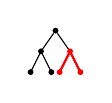
\begin{tikzpicture}[
baseline=-12, scale=0.5, every node/.style={dotA},
level distance=15pt,
level 1/.style={sibling distance=21 pt},
level 2/.style={sibling distance=\distC pt},
level 3/.style={sibling distance=15pt}
]
\node   (root) {}
child {child child} child {child child};
\node  at (root-1) {}; \node [color=red] at (root-2) {};
\node at (root-1-1) {}; \node at (root-1-2) {};
\node [color=red]  at (root-2-1) {}; \node [color=red] at (root-2-2) {};
\path  (root-2) edge [thick, color=red] (root-2-1) ;
\path  (root-2) edge [thick, color=red] (root-2-2) ;
\end{tikzpicture}
\ ,
\quad
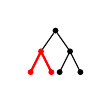
\begin{tikzpicture}[
baseline=-12, scale=0.5, every node/.style={dotA},
level distance=15pt,
level 1/.style={sibling distance=21 pt},
level 2/.style={sibling distance=\distC pt},
level 3/.style={sibling distance=15pt}
]
\node   (root) {}
child {child child} child {child child};
\node [color=red] at (root-1) {}; \node at (root-2) {};
\node [color=red]  at (root-1-1) {}; \node [color=red]  at (root-1-2)
{};
\node  at (root-2-1) {}; \node at (root-2-2) {};
\path  (root-1) edge [thick, color=red] (root-1-1) ;
\path  (root-1) edge [thick, color=red] (root-1-2) ;
\end{tikzpicture}
\ , \quad
\text{and}
\quad
\quad
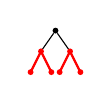
\begin{tikzpicture}[
baseline=-12, scale=0.5, every node/.style={dotA},
level distance=15pt,
level 1/.style={sibling distance=21 pt},
level 2/.style={sibling distance=\distC pt},
level 3/.style={sibling distance=15pt}
]
\node   (root) {}
child {child child} child {child child};
\node [color=red] at (root-1) {}; \node [color=red] at (root-2) {};
\node [color=red] at (root-1-1) {}; \node [color=red] at (root-1-2) {};
\node [color=red] at (root-2-1) {}; \node [color=red] at (root-2-2) {};
\path  (root-2) edge [thick, color=red] (root-2-1) ;
\path  (root-2) edge [thick, color=red] (root-2-2) ;
\path  (root-1) edge [thick, color=red] (root-1-1) ;
\path  (root-1) edge [thick, color=red] (root-1-2) ;
\end{tikzpicture}
\ .
\end{align}

\noi Analogously to the $v$ equation, we rewrite \eqref{w1} by combining terms with the same homogeneity in $w$ and associated with the same tree, thus moving the complexity to the corresponding multipliers. In this way, we do not need to consider coloured trees as in \eqref{Bcherry2}. More importantly, this process leads to a fundamental cancellation, since \textit{all the boundary terms cancel}, as shown in the following lemma.



%In particular, from \eqref{NFE1a} and \eqref{eq:defiB}, we see that
%\begin{align}
%& \B(\<33>) [w] (t) + \B(\<21>)\big[w, \D[w] \big](t) + \B(\<22>)\big[
%\D[w], w\big] (t) + \B( \<1>)  \big[ \D[w] \big] (t) \\
%& = \bigg[
%\int_{\G(\TT) } e^{it' \Psi(\TT)} w_{100}w_{101}w_{110}w_{111}
% \Big(  \mulB(\<33>) + \mulB(\<21>) \mulB(\cherry{11}{}{})  \\
%& \qquad \qquad
%+ \mulB(\<22>) \mulB(\cherry{10}{}{}) + \mulB(\<1>) \mulB(\cherry{10}{}{})  \mulB(\cherry{11}{}{})  \Big)
%d\vec\xi
%\bigg]_{t'=0}^{t'=t},
%\end{align}
%where we use the notation $\TT= \<33>$. Replacing \eqref{NFE0b} in the multiplier above, we see that
%\begin{align}
%& \mulB(\<33>) + \mulB(\<21>) \mulB(\cherry{11}{}{})
%+ \mulB(\<22>) \mulB(\cherry{10}{}{}) + \mulB(\<1>) \mulB(\cherry{10}{}{})  \mulB(\cherry{11}{}{})  \\
%& = \ind_{A_1^c, A_{10}^c, A_{11}^c} K_1 K_{10} K_{11} \Big( (-1)^{4} + (-1)^{3+2} + (-1)^{3+2} + (-1)^{2+2+2} \Big) = 0,
%\end{align}
%from which we conclude that there is no quartic in $w$ boundary term in \eqref{w1}. In fact, the following lemma establishes that all the boundary terms appearing in \eqref{w1} actually vanish, when grouped by homogeneity in $w$.





\begin{lemma}
\label{LEM:wbd}




Let $j\in\N$, $\TT\in \Tr_j$, 
$\star \in \TT^{0,\ff}$, and $w_1, \ldots, w_{j+1}: \R\times \R \to \R$ be any smooth functions. Moreover, consider the lexicographical ordering of the leaves of $\TT$ as in \eqref{lexic}, 
and let $1 \le k \le j$ be such that $(\bul_k, \bul_{k+1})$ are the children of $\star$ in $\TT$. 
Then, we have 
\begin{align}
\label{wbd0}
\BB\big(\TT ; w_1, \ldots, w_{j+1} \big) 
+ \BB\big(\TT\overset{\star}{\ominus} \<1>; w_1,  \ldots, w_{k-1} , \D[w_k,w_{k+1}] , w_{k+2}, \ldots,  w_{j+1} \big) 
\equiv 0.
\end{align}
%Consequently, 
%by combining all the contributions in \eqref{w1} with corresponding with the same tree (ignoring colourings), we also obtain cancellation:
%\begin{align}
%\sum_{A\subseteq \TT^{0,\ff}} \B \big( \TT \overset{A}{\ominus } \<1>; u_\bul = \D[w,w], \bul \in A, \ u_\bul = w \text{ otherwise} \big)
%\equiv 0
%.
%\end{align}
%where $\BB$ is as in \eqref{NFE1a}. 
Consequently, all the boundary terms in \eqref{w1} vanish:
\begin{multline}
\label{wbd1}
  \BB \big(\<1>; w, \D[w, w] \big) 
+ \BB\big(\<1>; \D[w, w],w\big) 
\\
+
\BB\big(\<1>;\D[w, w], \D[w, w]\big)
+ \sum_{j=2}^\infty \sum_{\TT\in \Tr_j}  \BB\big(\TT; w + \D[w, w]\big)  \equiv 0  .
\end{multline}


\end{lemma}




\begin{proof}

Let $j\in\N$, $\TT\in\Tr_j$, and $\star \in \TT^{0,\ff}$, and  consider the terminal nodes of $\TT$ ordered as in \eqref{lexic}. 
We start by showing \eqref{wbd0}. From \eqref{NFE1a} in Proposition~\ref{PRO:NFE} and \eqref{w}, we have
\begin{align}
&
\F_x\big[ 
\BB\big(\TT ; w_1, \ldots, w_{j+1} \big) 
+ \BB\big(\TT\overset{\star}{\ominus} \<1>; w_1,  \ldots, w_{k-1} , \D[w_k,w_{k+1}] , w_{k+2}, \ldots,  w_{j+1} \big) 
\big](t)
\\
&
=
-i\dt\bigg[
\int_{\G(\TT)} e^{it \Psi(\TT)} \mulB(\TT) \prod_{\l=1}^{j+1} \ft{w}_{\l} (t, \xi_{\bul_\l}) d\vec\xi
\\
&
\quad 
+
\int_{\G(\TT\overset{\star}{\ominus}\<1>)} \int_{\xi_{\star} = \xi_k + \xi_{k+1}} e^{it \Psi(\TT\overset{\star}{\ominus}\<1>) + it\Psi(\star)} \mulB(\TT\overset{\star}{\ominus}\<1>) \mulB(\cherry{\star}{}{}) \prod_{\l=1}^{j+1} \ft{w}_{\l} (t, \xi_{\bul_\l})  \, d\xi_k d\vec\xi
\bigg]
\\
&
= 
-i\dt\int_{\G(\TT)} 
e^{it\Psi(\TT)} 
\big\{ 
\mulB(\TT)
+
 \mulB(\TT\overset{\star}{\ominus}\<1>) \mulB(\cherry{\star}{}{})
\big\}
\prod_{\l=1}^{j+1} \ft{w}_{\l} (t, \xi_{\bul_\l}) d\vec\xi
\end{align}
where we used the additivity of $\Psi$ in \eqref{eq:additivity}. Replacing \eqref{NFE0b} in the multiplier above gives
\begin{align}
&
\mulB(\TT)
+
 \mulB(\TT\overset{\star}{\ominus}\<1>) \mulB(\cherry{\star}{}{})
\\
&
=
(-1)^{j+1} \prod_{\bul \in \TT^0} \ind_{A^c_\bul} K_\bul 
+
\bigg( (-1)^{j} \prod_{\bul\in \TT^0 \setminus \{\star\}} \ind_{A^c_\bul} K_\bul \bigg) 
\big( 
(-1)^2 \ind_{A^c_\star} K_\star
\big)
=0, 
\end{align}
since $(\TT \overset{\star}{\ominus} \<1>)^{0} = \TT^0 \setminus \{\star\}$, from which \eqref{wbd0} follows.

To show \eqref{wbd1}, let $j\in \N$ and $\TT \in \Tr_j$. Then, gathering all the boundary terms in \eqref{w1}
associated with the tree $\TT$ (when viewed as coloured trees as in \eqref{Bcherry2}), we have
\begin{align*}
\wt{\BB}(\TT; w)  & =
\sum_{ P\subseteq \TT^{0,f}  } \BB\Big(\TT\overset{P}{\ominus} \<1>;  f_{\bul} = w, \ \bul
\in (\TT\overset{P}{\ominus} \<1>)^\infty \setminus P , f_{\star} = \D[w,w] , \star \in P
\Big).
\end{align*}


Using \eqref{NFE1a}, \eqref{eq:defiI}, and \eqref{NFE0b}, we see that
\begin{align}
\wt{\BB}(\TT;w)   = \dt \Ical(\TT, \wt{\mul}_\BB (\TT);w )
\end{align}
where
\begin{align}
\label{wbd1a}
\begin{split}
\wt{\mul}_\BB(\TT)
 &
= \sum_{P\subseteq \TT^{0,\ff}} \mul_{\BB}\Big(\TT\overset{P}{\ominus} \<1>\Big)
\prod_{\star \in P} \mulB(\cherry{\star}{}{})
\\
&
= \sum_{P\subseteq \TT^{0,\ff}} (-1)^{|\TT^0| - |P| + 1} \bigg( \prod_{\bul \in \TT^0 \setminus P} \ind_{A_\bul^c } K_\bul \bigg) \bigg( \prod_{\star \in P} \ind_{A_\star^c} K_\star \bigg) \\
&
=(-1)^{|\TT^0|+1} \bigg( \prod_{\bul \in \TT^0} \ind_{A_\bul^c} K_\bul \bigg) \sum_{P \subseteq \TT^{0,\ff}} (-1)^{|P|} \\
&
=(-1)^{|\TT^0|+1} \bigg( \prod_{\bul \in \TT^0} \ind_{A_\bul^c} K_\bul \bigg) \sum_{k=0}^{|\TT^{0,\ff}|} \binom{|\TT^{0,\ff}|}{k} (-1)^{k} \\
& =0 ,
\end{split}
\end{align}
and the result follows. \qedhere

% given $j\in \N$ with $j\ge 2$, and $\TT \in \Tr_j$, we gather all the contributions on the right-hand side of \eqref{wbd1} which are represented by $\TT$ ignoring colourings:
% \begin{align}
% \label{wbd2a}
% \sum_{ C \subseteq \TT^{0,f}  } 
% \BB
% \Big(\TT \overset{C}{\ominus} \<1> ; \ f_{\bul} = w \  \text{ if } \ \bul
% \in (\TT\overset{C}{\ominus} \<1>)^\infty \setminus C ,  \ f_{\bul} = \D[w, w] \  \text{ if }  \ \bul \in C
% \Big) 
% , 
% \end{align}
% where the latter is to be interpreted as (i) evaluated at $w$ for the entries corresponding to terminal nodes in $ (\TT\overset{C}{\ominus} \<1>)^\infty \setminus C$, which corresponds to terminal nodes of $\TT$ which are not children of nodes in $C$; and (ii) evaluated at $\D[w,w]$ as given in \eqref{w} at the nodes in $A$. Note that the terms above have homogeneity $(j+1 - 2|C|) + 2|C| = j+1$, since $\D[w,w]$ contributes with two factors of $w$, and thus agreeing with the homogeneity of $\BB(\TT; w)$ which is included above when $C= \emptyset$. 

% Fix $\star \in \TT^{0,\ff}$. Then, we can split the sum in \eqref{wbd2a} between the terms with $\star \in C$ and $\star \not\in C$: for a given set $C$, let $C_\star = C\cup \{\star\}$, 
% \begin{multline}
% \sum_{ C \subseteq \TT^{0,f} \setminus\{\star\} } 
% \bigg\{
% \BB
% \Big(\TT \overset{C_\star}{\ominus} \<1> ; \ f_{\bul} = w \  \text{ if } \ \bul
% \in (\TT\overset{C_\star}{\ominus} \<1>)^\infty \setminus C_\star,  \ f_{\bul} = \D[w, w] \  \text{ if }  \ \bul \in C_\star
% \Big) 
% \\
% + 
% \BB
% \Big(\TT \overset{C}{\ominus} \<1> ; \ f_{\bul} = w \  \text{ if } \ \bul
% \in (\TT\overset{C}{\ominus} \<1>)^\infty \setminus C,  \ f_{\bul} = \D[w, w] \  \text{ if }  \ \bul \in C
% \Big) 
% \bigg\}. 
% \end{multline}
% Fixing a set $C$ in the sum, and using the notation $\wt\TT= \TT \overset{C}{\ominus} \<1>$, note that from \eqref{treeSubtr} in Definition~\ref{DEF:tree3}~(iii), we have
% $\TT \overset{C_\star}{\ominus} \<1> = \wt \TT \overset{\star}{\ominus} \<1>$.
% Moreover, $(\wt \TT \overset{\star}{\ominus} \<1>)^\infty \setminus C_\star = \wt\TT^\infty \setminus ( C \cup \{\star1, \star2\})$. Thus, we rewrite each summand above as
% \begin{align}
% &
% \BB \big( 
% \wt\TT \overset{\star}{\ominus} \<1>; 
%  f_{\bul} = w 
% \  \text{ if } \ \bul \in \wt\TT^\infty \setminus ( C \cup \{\star1, \star2\})
% ,  
% \ f_{\bul} = \D[w, w] \  \text{ if }  \ \bul \in C, \ f_\star = \D[w, w] 
% \big)
% \\
% &
% +
% \BB \big( 
% \wt\TT ;
%  f_{\bul} = w 
% \  \text{ if } \ \bul \in \wt\TT^\infty \setminus ( C \cup \{\star1, \star2\})
% ,  
% \ f_{\bul} = \D[w, w] \  \text{ if }  \ \bul \in C_\star ,
% \ f_{\star1} = f_{\star2} = w
% \big)
% \end{align}
% which vanishes, 
% since it is of the form in \eqref{wbd0}, with $(\bul_{k}, \bul_{k+1}) = (\star1, \star2)$. Summing over all choices of $C\subseteq \TT^{0,\ff}$, we obtain the cancellation for each tree $\TT \in \Tr_j$, and further summing over $j\ge 2$ gives \eqref{wbd1}. 





\end{proof}



We can then further rewrite the equation \eqref{w1} by grouping integral terms in a similar fashion. Similarly to Lemma~\ref{LEM:wbd} which establishes the cancellation of \textit{all} boundary terms in the $w$ equation \eqref{w1}, the next lemma also shows some cancellation for integral terms. 

\begin{lemma}
\label{LEM:wint}
Let $w:\R \times \R\to \R$ be a smooth function and $\NN$ be as in \eqref{NFE1a}.
Then, we have
\begin{align}
\label{wint0a}
%  \NN\big(\<1>; w,w \big)  + \NN\big(\<1>; w, \D[w, w]\big)+
%\NN\big(\<1>;\D[w, w], w\big) + \NN\big(\<1>; \D[w, w],\D[w, w]\big) \\
%+ 
\sum_{j=1}^\infty \sum_{\TT\in \Tr_j} \NN\big(\TT; w+
\D[w, w]
\big)
=
\NN_1(\<1>;w) + \sum_{j=2}^\infty \sum_{\TT\in\Tr_j} \sum_{\ell=2}^4  \NN_\ell(\TT; w),
\end{align}
where the nonlinear contributions are defined via their spatial Fourier transform
\begin{align}
\label{wint0b}
\begin{split}
\Ft_x \big[ \NN_\ell (\TT; w) \big] & =
\Ical \big(\TT, {\mul}_\l(\TT); w \big),\quad \l=1,\dots, 4,
% , \\
% \Ft_x \big[ \NN^\bfrak (\TT; w) \big] (t,\xi) & =
% \Ical \big(\TT, {\mul}_\bfrak(\TT) ; w \big) (t), 
\end{split}
\end{align}
for $\Ical(\TT, m; w)$ as in \eqref{eq:defiI}, 
%where the multipliers of the first trees are given by
%
%\begin{align}
%\label{wint0bb}
%\begin{aligned}
%\mul_{\gfrak}(\<1>)
%& %= \mul(\<1>)
%= K \ind_A \Psi(\<1>)
%, 
%&
%\mul_{\bfrak}(\<1>)
%&
%=
%0
%, 
%\\
%%%%%%%%%
%\mul_{\gfrak}(\<21>)
%& 
%=
%- KK_1\big( \ind_{A^c,A_1} \Psi(1) 
%- \ind_{A, A_1^c} \Psi(\<1>)
%\big)
%,
%&
%\mul_{\bfrak}(\<21>)
%&
%=  KK_1 \ind_{A^c, A_1^c} \Psi(\<1>)
%, 
%\\
%%%%%%%%%
%\mul_{\gfrak}(\<22>)
%& 
%=
%- KK_2\big( \ind_{A^c,A_2} \Psi(2) 
%- \ind_{A, A_2^c} \Psi(\<1>)
%\big)
%,
%&
%\mul_{\bfrak}(\<22>)
%&
%=  KK_2 \ind_{A^c, A_2^c} \Psi(\<1>)
%, 
%\\
%%%%%%%%%
%\mul_{\gfrak}(\<33>)
%&
%= K K_{1} K_{2} \ind_{A, A_{1}^c, A_{2}^c} \Psi(\<1>)
%,
%&
%\mul_{\bfrak}(\<33>)
%&
%= K K_{1} K_{2} \ind_{A^c, A_{1}^c, A_{2}^c} \Psi(\<1>)
%,
%\end{aligned}
%\end{align}
where the multipliers are given by %and $\TT\neq \<33>$ 
\begin{align}
    \mul_1(\<1>)&= \ind_A K \Psi(\<1>),\\
    \mul_2(\TT)&=(-1)^{j+1} \ind_{A_\star} K_\star\Psi(\star) \bigg( \prod_{\bul \in \TT^0 \setminus\{\star\}}  K_\bul  \ind_{A_\bul^c} \bigg), 
    && \text{if} \quad  \TT^{0,\ff} = \{\star\}, \ \star\neq \emptyset, 
    \\
    \mul_3(\TT)&=(-1)^{j}  K_{\pb(\star)}\Psi(\pb(\star)) \bigg( \prod_{\bul \in \TT^0 \setminus\{\pb(\star)\}}  K_\bul  \ind_{A_\bul^c} \bigg),
    &&
    \text{if} \quad  \TT^{0,\ff} = \{\star\},  \ \star\neq \emptyset
    \label{wint0c}
    \\
     \mul_4(\TT)&=(-1)^{j+1}  K_\star\Psi(\star) \bigg( \prod_{\bul \in \TT^0 \setminus\{\star\}}  K_\bul  \ind_{A_\bul^c} \bigg), 
    && \text{if} \quad  \TT^{0,\ff} = \{\star1, \star2\}, 
    \\
    \mul_{\l}(\TT) & = 0, \ \l=2,3,4 && \text{otherwise}, 
\end{align}
with $\TT\in \Tr_j$,  $j \ge 2$, and $K$ and $\Psi$ as in \eqref{Kmul} and \eqref{psi-tree}, respectively.
Moreover, for $\l=1,\ldots, 4$, we will refer to the contributions $\NN_\l(\TT) $ as terms of Type $\I,\II,\III,\IV$, respectively. 


% \begin{align}
% \mul_{\gfrak}(\<1>)
% & %= \mul(\<1>)
% = K \ind_A \Psi(\<1>)
% , 
% \\
% \mul_{\bfrak}(\<1>)
% &
% =
% 0
% ,
% \\
% \mul_\gfrak(\TT)
% &
% =
% (-1)^{j+1} \bigg( \prod_{\bul \in \TT^0} K_\bul  \bigg)
% \\
% &\quad 
% \times
% \begin{cases}
% \displaystyle
% \ind_{A_\star} \Psi(\star) \bigg( \prod_{\bul \in \TT^0 \setminus\{\star\}} \ind_{A_\bul^c} \bigg) - \ind_{A_{\pb(\star)}} \Psi(\pb(\star)) \bigg( \prod_{\bul \in \TT^0 \setminus\{\pb(\star)\}} \ind_{A_\bul^c} \bigg)
% ,
% & \text{if } \TT^{0,\ff} = \{\star\} , 
% \\
% \displaystyle
% \ind_{A_\star} \Psi(\star) \bigg( \prod_{\bul \in \TT^0 \setminus\{\star\}} \ind_{A_\bul^c} \bigg) ,
% & \text{if } \TT^{0,\ff} = \{\star1, \star2\} , 
% \\
% 0, & \text{if } |\TT^{0,\ff}|\ge 3, 
% \end{cases}
% \\
% \mul_{\bfrak}(\TT)
% &
% = (-1)^{j+1} \bigg( \prod_{\bul \in \TT^0} \ind_{A_\bul^c} K_\bul \bigg)
% \times
% \begin{cases}
% - \Psi(\pb(\star)) 
% , &
% \text{if } \TT^{0,\ff} = \{\star\} , 
% \\
% \Psi(\star)
% , &
% \text{if } \TT^{0,\ff} = \{\star1,\star2\} , 
% \\
% 0, & \text{if } |\TT^{0,\ff}|\ge 3
% ,
% \end{cases}
% \label{wint0c}
% \end{align}
 

% \color{blue}
% \andreia{Alternative form. More compact, but more difficult to decipher?}
% \begin{align}
% \mul_\gfrak(\TT)
% &
% = (-1)^{j+1} \bigg( \prod_{\bul \in \TT^0} K_\bul  \bigg)
% \sum_{\star \in \TT^0} \ind_{A_\star} \Psi(\star) \bigg( \prod_{\bul \in \TT^0 \setminus \{\star\}} \ind_{A_\bul^c} \bigg) \\
% &
% \quad \times \Big( \ind_{\TT^{0,\ff} = \{\star\}} + \ind_{\TT^{0,\ff} = \{\star1,\star2\}} - \ind_{\TT^{0,\ff} = \{\star1\}} - \ind_{\TT^{0,\ff} = \{\star2\}} \Big),
% \\
% \mul_{\bfrak}(\TT)
% &
% = (-1)^{j+1} \bigg( \prod_{\bul \in \TT^0} \ind_{A_\bul^c} K_\bul \bigg)
% \sum_{\star \in \TT^0 \setminus \TT^{0,\ff}} \Psi(\star)
% \Big( \ind_{\TT^{0,\ff} = \{\star1, \star2\}} - \ind_{\TT^{0,\ff} = \{\star1\}} - \ind_{\TT^{0,\ff} = \{\star2\}} \Big),
% \end{align}

\end{lemma}



\begin{proof}


We note that there is a unique element on l.h.s. of \eqref{wint0a} with homogeneity 2 in $w$, namely $\NN(\<1>; w,w)$.
Therefore, $\NN_1(\<1>;w) = \NN(\<1>;w)$ and $\mul_1(\<1>) = \mul(\<1>)$ as in \eqref{NFE1a}-\eqref{NFE0b}. 

Next, we consider the contributions on the l.h.s. of \eqref{wint0a} with underlying tree structure of $\<21>$, $\<22>$, and $\<33>$.  
Namely, from \eqref{wint0a}, \eqref{NFE1a}, and \eqref{NFE0b}, we have
\begin{align}
&
		\NN(\<1>; \D[w, w], w) + \NN(\<21>; w) \\
		&
		=  \Ical \Big(\<21>, - K K_{1} \big(   \ind_{A^c\cap A_{1}} \Psi(1) - \ind_{A^c\cap A_{1}^c} \Psi(\<1>)  \big); w \Big)
		+
		\Ical \Big(\<21>, K K_{1}  \ind_{A\cap A_{1}^c} \Psi(\<1>); w \Big)
\\
& 
=  \Ical \Big(\<21>, - K K_{1}   \ind_{A^c\cap A_{1}} \Psi(1) ; w \Big)
		+
		\Ical \Big(\<21>, K K_{1}  \ind_{ A_{1}^c} \Psi(\<1>); w \Big)
\\
&
= : \NN_2(\<21>; w) + \NN_3(\<21>; w )
,
\\
% &
% =: \NN^{\gfrak} (\<21>; w) + \NN^{\bfrak}(\<21>; w)
% 		,
% 		\\
&
		\NN(\<1>; w, \D[w, w] ) + \NN(\<22>; w) \\
		&
		=  \Ical \Big(\<22>, - K K_{2} \big(   \ind_{A^c\cap A_{2}} \Psi(2) - \ind_{A^c\cap A_{2}^c} \Psi(\<1>)  \big); w \Big)
		+
		\Ical \Big(\<22>, K K_{2}  \ind_{A\cap A_{2}^c} \Psi(\<1>); w \Big)
\\
&
=
\Ical \Big(\<22>, - K K_{2}   \ind_{A^c\cap A_{2}} \Psi(2) ; w \Big)
		+
		\Ical \Big(\<22>, K K_{2}  \ind_{ A_{2}^c} \Psi(\<1>); w \Big)
\\
&
=: 
\NN_2 (\<22>; w) + \NN_3 (\<22>; w)
,
\\
% &
% =: \NN^{\gfrak} (\<22>; w) + \NN^{\bfrak}(\<22>; w)
% , 
% 	\\
&
		\NN(\<1>;  \D[w, w], \D[w, w] ) + \NN(\<21>; w,w,  \D[w, w])  + \NN(\<22>; \D[w, w],w, w) + \NN(\<33>;w)  \\
		&
		=
		\Ical \Big( \<33>, KK_1K_2 \Psi(\<1>) \ind_{A\cap A_{1}^c\cap A_{2}^c}  \Big)
		+\Ical \Big( \<33>, KK_1K_2 \Psi(\<1>) \ind_{A^c\cap A_{1}^c\cap A_{2}^c}  \Big)
        \\
        \color{red}
        &
		=
		\Ical \Big( \<33>, KK_1K_2 \Psi(\<1>) \ind_{ A_{1}^c\cap A_{2}^c}  \Big)
\\
&
=: \NN_4 (\<33>; w) 
, 
	\end{align}

\noi
where we note the agreement with \eqref{wint0b}-\eqref{wint0c}.

	


	
	Now let $j\in\N$ with $j\ge3$ and $\TT\in \Tr_j$, such that $\TT \neq \<33>$.
	We write the resulting term corresponding to tree $\TT$ by  gathering the integral terms in \eqref{wint0a}
	associated with the tree $\TT$ without colourings:
	\begin{align*}
		\sum_{ C \subseteq \TT^{0,f}  } \NN\big(\TT \overset{C}{\ominus} \<1> ;  
		f_{\bul} = w \ \text{ if }\ \bul \in (\TT\overset{C}{\ominus}\<1>)^\infty \setminus C , \
		 f_{\bul} = \D[w, w] \ \text{ if } \ \bul \in C
		\big)
		 = \Ical ( \TT, \wt{\mul}(\TT); w),
	\end{align*}
	where $\Ical$ is as in \eqref{eq:defiI} and the multiplier $\wt{\mul}(\TT)$ is given by
	\begin{align}
			\wt{\mul}(\TT) 
		& = \sum_{C \subseteq \TT^{0,\ff}} \mul(\TT\overset{C}{\ominus} \<1>)
			\bigg( \prod_{\star \in C } \mulB(\cherry{\star}{}{}) \bigg)
			\\
			& = \sum_{C \subseteq \TT^{0,\ff}} (-1)^{ j + 1 + |C|}
			\bigg( \prod_{\bul\in \TT^0 \setminus C    } K_\bul \bigg)
			\bigg(\prod_{\star \in C} \ind_{A_\star^c} K_\star \bigg) \\
			& \quad \times \bigg\{ \sum_{\star \in (\TT \overset{C}{\ominus} \cherryS)^{0,\ff}} \ind_{A_\star} \Psi(\star) 
			\bigg(\prod_{\bul \in \TT^0 \setminus(C \cup \{\star\})} \ind_{A_\bul^c} \bigg)
			- 
			\bigg(\prod_{\bul \in \TT^0 \setminus C} \ind_{A_\bul^c}\bigg) 
			\sum_{\star \in (\TT \overset{C}{\ominus} \cherryS)^0  \setminus (\TT \overset{C}{\ominus} \cherryS)^{0,\ff}} \Psi(\star) 
			\bigg\} \\
			& =: {\mul}_{\gfrak}(\TT) + {\mul}_{\bfrak}(\TT),
		\label{wint1a}
	\end{align}
	where we used \eqref{NFE0b}, and the fact that $(\TT\overset{C}{\ominus}\<1>)^0 = \TT^0 \setminus C$. It remains to simplify the multipliers above.




	We first consider ${\mul}_{\bfrak}(\TT)$, which we write as 
	\begin{align}
		{\mul}_{\bfrak} (\TT) 
%& =
%			(-1)^j \bigg( \prod_{\bul \in \TT} \ind_{A_\bul^c} K_\bul \bigg) \sum_{C \subseteq \TT^{0,\ff}} (-1)^{|C|} \sum_{\star\in(\TT \overset{C}{\ominus} \cherryS)^0  \setminus (\TT \overset{C}{\ominus} \cherryS)^{0,\ff}} \Psi(\star) 
%	\\
&
= (-1)^j \bigg( \prod_{\bul \in \TT} \ind_{A_\bul^c} K_\bul \bigg)
\sum_{\star \in \TT^0 } \Psi(\star) \sum_{ C \subseteq \TT^{0,\ff}} (-1)^{|C|} \ind_{\star\in (\TT \overset{C}{\ominus} \cherryS)^0  \setminus (\TT \overset{C}{\ominus} \cherryS)^{0,\ff}},
	\label{wint2a}
	\end{align}
where it remains to simplify the latter sum, by considering different cases for $\star$. 
Note that if $\star \in \TT^{0,\ff}$ or $\star\in \TT^0\setminus \TT^{0,\ff}$ with at least one child in $\TT^0 \setminus \TT^{0,\ff}$, then sum over all $C\subseteq \TT^{0,\ff}$ in \eqref{wint2a} gives a zero contribution. Thus, it remains to consider $\star \in \TT^0 \setminus \TT^{0,\ff}$ and $\{\star1, \star2\} \subseteq \TT^{0,\ff} \cup \TT^\infty$, noting that we cannot have both children being leaves.

% \smallskip 
% \noi
% \underline{\textbf{Case 0}: (a) $\star\in \TT^{0,\ff}$ or (b) $\star \in \TT^{0}\setminus\TT^{0,\ff}$ and $\{\star1, \star2\}\cap \TT^{0}\setminus\TT^{0,\ff} \neq \emptyset$ }

% If (a) holds, then regardless of the choice of $C$ in \eqref{wint2a}, $\star \not\in (\TT \overset{C}{\ominus} \cherryS)^0  \setminus (\TT \overset{C}{\ominus} \cherryS)^{0,\ff}$ as it is either a final node or a final parent in the new tree. Thus, this always contributes with 0. 
%
% This is analogous if (b) holds, since every choice of $C$ in \eqref{wint2a} leads to zero contribution. 


\smallskip 

\noi
\underline{\textbf{Case 1}:  $(\star1, \star2) \in \TT^{0,\ff} \times \TT^\infty$ or $(\star1, \star2) \in \TT^\infty \times \TT^{0,\ff}$}


If 
$(\star1, \star2) \in \TT^{0,\ff} \times \TT^\infty$, then the only non-zero contributions in the sum over $C$ in \eqref{wint2a} are
\begin{align}
\sum_{C\subseteq \TT^{0,\ff} \setminus \{\star1\}} (-1)^{|C|}
=  \sum_{j=0}^{|\TT^{0,\ff}|-1} \binom{|\TT^{0,\ff}|-1}{j} (-1)^j
=  \ind_{|\TT^{0,\ff}| = 1},
\end{align}
and we must have $\TT^{0,\ff} = \{\star 1\}$ to have a non-zero term. The remaining case is analogous by symmetry between $\star1$ and $\star2$. 


\smallskip 
\noi
\underline{\textbf{Case 2}:  $\star1,\star2\in \TT^{0,\ff}$}

In this case, $C$ can contain at most one element in $\{\star1,\star2\}$, thus we get
\begin{align}
 \sum_{C\subseteq \TT^{0,\ff} \setminus\{\star1,\star2\}}[ (-1)^{|C|}  + (-1)^{|C|+1} + (-1)^{|C|+1}]
=
-  \ind_{|\TT^{0,\ff}| = 2}
\end{align}
which is nonzero when $\TT^{0,\ff} = \{\star1, \star2\}$. 

Combining the different cases, we get
\begin{align}\label{mulb}
\mul_{\bfrak}(\TT) = (-1)^{j+1} \bigg( \prod_{\bul \in \TT^0} \ind_{A_\bul^c} K_\bul \bigg) \sum_{\star\in\TT^0\setminus\TT^{0,\ff}}\Psi(\star)
\big( 
- \ind_{\TT^{0,\ff} = \{\star1\}} - \ind_{\TT^{0,\ff} = \{\star2\}} + \ind_{\TT^{0,\ff} = \{\star1, \star2\}}
\big).
\end{align}



	
	We now consider the first multiplier ${\mul}_\gfrak$ in \eqref{wint1a}, which we rewrite as follows
	\begin{align}
    \begin{split}
		 {\mul}_\gfrak (\TT) 
%		& = \sum_{P\subseteq \TT^{0,\ff}} (-1)^{|\TT^0| + |P| + 1}
%		\bigg( \prod_{\bul\in (\TT \setminus P)^0 } K_\bul \bigg)
%		\bigg(\prod_{\circ \in P} \ind_{A_\circ^c} K_\circ \bigg)  \sum_{\star \in (\TT\setminus P)^{0,\ff}} \ind_{A_\star} \Psi(\star) \bigg(\prod_{\bul \in \TT^0 \setminus \{\star\} } \ind_{A_\bul^c} \bigg)
%		\\
		&
		=
(-1)^{j+1}
		\bigg( \prod_{\bul \in \TT^0} K_\bul \bigg) 
		\sum_{ C \subseteq \TT^{0,\ff}} (-1)^{|C|}  \sum_{\star \in (\TT \overset{C}{\ominus} \cherryS)^{0,\ff}}  \ind_{A_\star} \Psi(\star) \bigg(\prod_{\bul \in \TT^0\setminus\{\star\}} \ind_{A_\bul^c} \bigg)\label{wint3a}
\\
&
=
(-1)^{j+1}
		\bigg( \prod_{\bul \in \TT^0} K_\bul \bigg) 
 \sum_{\star \in \TT^0} \ind_{A_\star} \Psi(\star)
		\bigg( \prod_{\bul\in\TT^0 \setminus\{\star\}} \ind_{A_\bul^c}\bigg)
		\sum_{C\subseteq \TT^{0,\ff}} (-1)^{|C|} \ind_{\star \in (\TT\overset{C}{\ominus}\cherryS)^{0,\ff} } .
        \end{split}
	\end{align}
As before, we consider different cases depending on $\star$ and focus on the inner sum in $C$. 
Note that any $\star \in \TT^{0}\setminus \TT^{0,\ff}$ with at least one child in $\TT^0\setminus\TT^{0,\ff}$ gives a zero contribution in \eqref{wint3a}. Thus, we consider $\star \in \TT^{0,\ff}$ or $\{\star1,\star2\} \subseteq \TT^{0,\ff} \cup \TT^\infty$. 



% \smallskip 

% \noi\underline{\textbf{Case 0}: $\star \in \TT^{0}\setminus\TT^{0,\ff}$ and $\{\star1, \star2\}\cap \TT^{0}\setminus\TT^{0,\ff} \neq \emptyset$ }

% All choices of $C$ in \eqref{wint3a} give a zero summand, thus these choices of $\star$ give zero contribution. 



 
\smallskip 

\noi
\underline{\textbf{Case 1}: $\star\in \TT^{0,\ff}$  }

The inner summand in \eqref{wint3a} is non-zero when $C\subseteq \TT^{0,\ff} \setminus \{\star\}$:
\begin{align}
\sum_{C\subseteq \TT^{0,\ff} \setminus\{\star\}} (-1)^{|C|} = \ind_{|\TT^{0,\ff}|=1}, 
\end{align}
thus we need $\TT^{0,\ff} = \{\star\}$ to get a non-zero contribution. 


\smallskip 
\noi
\underline{\textbf{Case 2}:  $(\star1, \star2) \in \TT^{0,\ff} \times \TT^\infty$ or $(\star1, \star2) \in \TT^\infty \times \TT^{0,\ff}$}

If $(\star1, \star2) \in \TT^{0,\ff} \times \TT^\infty$,
the inner summand in \eqref{wint3a} is non-zero when $ \star1 \in C$, which gives
\begin{align}
\sum_{C\subseteq \TT^{0,\ff} \setminus\{\star1\}} (-1)^{|C|+1} = - \ind_{|\TT^{0,\ff}|=1}, 
\end{align}
thus we need $\TT^{0,\ff} = \{\star1\}$ to get a non-zero contribution. This is analogous for the other case by symmetry.

\smallskip 

\noi
\underline{\textbf{Case 3}:  $\star1,\star2\in \TT^{0,\ff}$}

In this case, we need $C$ in \eqref{wint3a} containing both $\star1$ and $\star2$, which gives
\begin{align}
\sum_{C\subseteq \TT^{0,\ff} \setminus\{\star1, \star2\}} (-1)^{|C|+2} = \ind_{|\TT^{0,\ff}|=2}, 
\end{align}
thus we need $\TT^{0,\ff} = \{\star1, \star2\}$ to get a non-zero contribution.

Combining the different terms, we get
\begin{align}\label{mulg}
{\mul}_\gfrak (\TT) 
& =
(-1)^{j+1}
		\bigg( \prod_{\bul \in \TT^0} K_\bul \bigg) 
 \sum_{\star \in \TT^0} \ind_{A_\star} \Psi(\star)
		\bigg( \prod_{\bul\in\TT^0 \setminus\{\star\}} \ind_{A_\bul^c}\bigg)
\\
&
\quad \times 
 \big( 
\ind_{ \TT^{0,\ff}  = \{\star\}} 
- \ind_{ \TT^{0,\ff}  = \{\star1\}}  
- \ind_{ \TT^{0,\ff}  = \{\star2\}} 
+\ind_{ \TT^{0,\ff}  = \{\star1, \star2\}}
\big).
\end{align}


Then, from \eqref{mulb} and \eqref{mulg}, we obtain
\begin{align}
    & 
     \mul_\bfrak (\TT) + \mul_\gfrak(\TT) 
     \\
&
= 
(-1)^{j+1}
\sum_{\star\in \TT^0} K_\star \Psi(\star)
\bigg( \prod_{\bul \in \TT^0 \setminus \{\star\}} K_\bul \ind_{A^c_\bul} \bigg)
\bigg(
\ind_{A_\star^c}  
\big( 
- \ind_{\TT^{0,\ff} = \{\star1\}} - \ind_{\TT^{0,\ff} = \{\star2\}} + \ind_{\TT^{0,\ff} = \{\star1, \star2\}}
\big)
\\
&
\hspace{3cm}
+
\ind_{A_\star} 
\big( 
\ind_{ \TT^{0,\ff}  = \{\star\}} 
- \ind_{ \TT^{0,\ff}  = \{\star1\}}  
- \ind_{ \TT^{0,\ff}  = \{\star2\}} 
+\ind_{ \TT^{0,\ff}  = \{\star1, \star2\}}
\big)
\bigg)
\\
&
= 
(-1)^{j+1}
\sum_{\star\in \TT^0} K_\star \Psi(\star)
\bigg( \prod_{\bul \in \TT^0 \setminus \{\star\}} K_\bul \ind_{A^c_\bul} \bigg)
\bigg(
\ind_{A_\star}
\ind_{\TT^{0,\ff} = \{\star\}}
-
\ind_{\TT^{0,\ff}=\{\star\l\}, \l=1,2 }
+
\ind_{\TT^{0,\ff} = \{\star1,\star2\}}
\bigg)
\\
&
= : \mul_2(\TT) + \mul_3(\TT) + \mul_4(\TT)
\label{mul234}
\end{align}

\noi 
which can be rewritten as in \eqref{wint0c}.
\qedhere


	
\end{proof}


 


% Similarly to Lemma~\ref{LEM:wbd} which establishes the cancellation of \textit{all} boundary terms in the $w$ equation \eqref{w1}, Lemma~\ref{LEM:wint} also shows some cancellation for time-integral terms. In particular, from \eqref{wint0c}, we see that the only trees with nonzero contributions are of one of the following 6 types listed in the following corollary.

% % \begin{corollary}\label{COR:types}
% % Given a smooth function $w$, $\NN$ as in \eqref{NFE1a}, and $\NN^\gfrak,\NN^\bfrak$ as in \eqref{wint0b},  we have that
% % \begin{align}
% % \sum_{j=1}^\infty \sum_{\TT\in \Tr_j} \NN\big(\TT; w+
% % \D[w, w]
% % \big)
% % =
% % \sum_{j=1}^\infty \sum_{\substack{\TT\in\Tr_j\\(\ast)}}  \NN^\gfrak(\TT; w)
% % +
% %  \sum_{j=1}^\infty \sum_{\substack{\TT\in\Tr_j\\(\ast\ast)}}  \NN^\bfrak(\TT; w), 
% % \end{align}
% % where the sums on the right-hand sided are restricted to the following 6 types of trees:
% % For the sum in $(\ast)$, we have
% % \begin{itemize}
% % 	\item \textup{Type I:} $\TT = \<1>$\,, %$\TT^{0,f}=\{\emptyset\}$, 
% % 	\item \textup{Type II:} $\TT^{0,f}=\{\star\}$ and $\star\neq\emptyset$,
% % 	\item \textup{Type III:} $\TT^{0,f}=\{\star1\}$ or $\TT^{0,f}=\{\star2\}$, 
% % 	\item \textup{Type IV:} $\TT^{0,f}=\{\star1,\star2\}$, 
% % \end{itemize}
% % while the sum in $(\ast\ast)$ includes terms of two types:
% % \begin{itemize}
% % \item \textup{Type V:}  $\TT^{0,f} = \{\star\}$ and $\star \neq \emptyset$,
% % \item \textup{Type VI:}  $\TT^{0,f} = \{\star1, \star2\}$. 
% % \end{itemize}

% % \end{corollary}


% Figure~\ref{FIG:types} provides examples for trees of Type I--IV, with the identification of the node $\star$ where the contribution is localized on the set $A_\star$ (see \eqref{defA}). Note that there is a unique tree of Type I. Moreover, trees of Type V and Type VI have the same graphical representation as those of Types II-III and Type IV (see Figure~\ref{FIG:types}(B)-(C) and (D)), respectively, ignoring the role of the node $\star$. 
% \begin{figure}[!h]
% \begin{subfigure}[b]{0.2\textwidth}
% \centering
% \begin{tikzpicture}[
% baseline=-15, scale=1, every node/.style={dotA},
% level distance=17pt,
% sibling distance=20pt,
% %level 1/.style={sibling distance=20pt},
% %level 2/.style={sibling distance=20 pt},
% %level 3/.style={sibling distance=20 pt},
% level 4/.style={sibling distance=15 pt}
% ]
% \node  [label=above:{}]  (root) {}
% child 
% child ;
% \node  at (root-1) {};
% \node  at (root-2) {};
% \path  (root-1) edge [ dotted, color=black] (root-1-1) ;
% \node 
% [label={[label distance=-3pt]above:$\star$}, circle ,fill=white, draw=black,  inner sep=1.5pt
% ] at (root) {};
% \end{tikzpicture}
% \caption{Type I.}
% \end{subfigure}
% %
% \begin{subfigure}[b]{0.2\textwidth}
% \centering
% \begin{tikzpicture}[
% baseline=-15, scale=1, every node/.style={dotA},
% level distance=17pt,
% sibling distance=20pt,
% %level 1/.style={sibling distance=20pt},
% %level 2/.style={sibling distance=20 pt},
% %level 3/.style={sibling distance=20 pt},
% %level 4/.style={sibling distance=20 pt}
% ]
% \node  [label=above:{}]  (root) {}
% child {
% 	child 
% 	{
% 		edge from parent[draw=none]
% %		edge from parent[dashed]
% 		child 
% 			{
% 			child  
% 			child
% 			}  
% %		edge from parent[draw=none]
% 		child
% 	} 
% 	child
% 	{edge from parent[draw=none]}
% }
% child {};
% \node at (root) {};
% \node  at (root-1) {};
% \node  at (root-2) {};
% \node at (root-1-1) {};
% \node at (root-1-1-2) {};
% \node at (root-1-1-1-2) {};
% \node  at (root-1-1-1-1) {};
% \node %[label=above:{}, transform shape,star, star points=6, star point ratio=.4, fill=white,inner sep=1.5pt, label distance=-1pt]  
% [label={[label distance=-3pt]above:$\star$}, circle ,draw=black, fill=white, inner sep=1.5pt
% %,minimum size=7pt
% ] at (root-1-1-1) {};
% \path  (root-1) edge [ dotted, color=black] (root-1-1) ;
% \end{tikzpicture}
% \caption{Type II.}
% \end{subfigure}
% %
% \begin{subfigure}[b]{0.2\textwidth}
% \centering
% \begin{tikzpicture}[
% baseline=-15, scale=1, every node/.style={dotA},
% level distance=17pt,
% sibling distance=20pt,
% %level 1/.style={sibling distance=20pt},
% %level 2/.style={sibling distance=20 pt},
% %level 3/.style={sibling distance=20 pt},
% %level 4/.style={sibling distance=20 pt}
% ]
% \node  [label=above:{}]  (root) {}
% child {
% 	child 
% 	{
% 		edge from parent[draw=none]
% %		edge from parent[dashed]
% 		child 
% 			{
% 			child  
% 			child
% 			}  
% %		edge from parent[draw=none]
% 		child
% 	} 
% 	child
% 	{edge from parent[draw=none]}
% }
% child {};
% \node at (root) {};
% \node  at (root-1) {};
% \node  at (root-2) {};
% \path  (root-1) edge [ dotted, color=black] (root-1-1) ;
% \node %[label=above:{}, transform shape,star, star points=6, star point ratio=.4, fill=white,inner sep=1.5pt, label distance=-1pt]  
% [label={[label distance=-2pt]above left:\footnotesize$\star1$}, circle ,draw=black, inner sep=1.5pt
% %,minimum size=7pt
% ] at (root-1-1-1) {};
% \node at (root-1-1-2) {};
% \node at (root-1-1-1-2) {};
% \node  at (root-1-1-1-1) {};
% \node %[label=above:{}, transform shape,star, star points=6, star point ratio=.4, fill=white,inner sep=1.5pt, label distance=-1pt]  
% [label={[label distance=-3pt]above:$\star$}, circle ,draw=black, fill=white, inner sep=1.5pt
% %,minimum size=7pt
% ] at (root-1-1) {};
% \end{tikzpicture}
% \caption{Type III.}
% \end{subfigure}
% %
% \begin{subfigure}[b]{0.2\textwidth}
% \centering
% \begin{tikzpicture}[
% baseline=-15, scale=1, every node/.style={dotA},
% level distance=17pt,
% sibling distance=20pt,
% %level 1/.style={sibling distance=20pt},
% %level 2/.style={sibling distance=20 pt},
% %level 3/.style={sibling distance=20 pt},
% level 4/.style={sibling distance=15 pt}
% ]
% \node  [label=above:{}]  (root) {}
% child {
% 	child 
% 	{
% 		edge from parent[draw=none]
% %		edge from parent[dashed]
% 		child 
% 			{
% 			child  
% 			child
% 			}  
% %		edge from parent[draw=none]
% 		child
% 			{
% 			child  
% 			child
% 			}  
% 	} 
% 	child
% 	{edge from parent[draw=none]}
% }
% child {};
% \node at (root) {};
% \node  at (root-1) {};
% \node  at (root-2) {};
% \path  (root-1) edge [ dotted, color=black] (root-1-1) ;
% \node 
% [label={[label distance=-3pt]above:$\star$}, circle ,fill=white, draw=black,  inner sep=1.5pt
% ] at (root-1-1) {};
% \node at (root-1-1-2) {};
% \node at (root-1-1-1-2) {};
% \node  at (root-1-1-1-1) {};
% \node at (root-1-1-2-2) {};
% \node  at (root-1-1-2-1) {};
% \node 
% [label={[label distance=-2pt]above left:\footnotesize$\star1$}, circle ,draw=black,  inner sep=1.5pt
% ] at (root-1-1-1) {};
% \node 
% [label={[label distance=-2pt]above right:\footnotesize$\star2$}, circle ,draw=black, inner sep=1.5pt
% ] at (root-1-1-2) {};
% \end{tikzpicture}
% \caption{Type IV.}
% \end{subfigure}
% \caption{Graphical representation of tree of Type I, and examples of trees of Types II--IV. }
% \label{FIG:types}
% \end{figure}

% \noi
% Lastly, note that from the definition of $\mul_{\gfrak}(\TT)$ in \eqref{wint0c}, for the same tree $\TT$, there is a contribution corresponding to Type II and another to Type III, when there is a restriction to $A_\star$ or $A_{\pb(\star)}$, respectively. 



\begin{remark} \rm
(i)
     From \eqref{wint0c}, we see that the only trees with nonzero contributions are, up to permutations, as depicted in Figure \ref{FIG:types}.


\begin{figure}[!h]
\begin{subfigure}[b]{0.2\textwidth}
\centering
\begin{tikzpicture}[
baseline=-15, scale=1, every node/.style={dotA},
level distance=17pt,
sibling distance=20pt,
%level 1/.style={sibling distance=20pt},
%level 2/.style={sibling distance=20 pt},
%level 3/.style={sibling distance=20 pt},
level 4/.style={sibling distance=15 pt}
]
\node  [label=above:{}]  (root) {}
child 
child ;
\node  at (root-1) {};
\node  at (root-2) {};
\path  (root-1) edge [ dotted, color=black] (root-1-1) ;
\node 
% [label={[label distance=-3pt]above:$\star$}, circle ,fill=white, draw=black,  inner sep=1.5pt
% ] 
at (root) {};
\end{tikzpicture}
\caption{Type $\I$.}
\end{subfigure}
%
\begin{subfigure}[b]{0.2\textwidth}
\centering
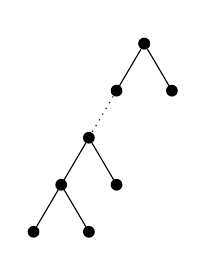
\begin{tikzpicture}[
baseline=-15, scale=1, every node/.style={dotA},
level distance=17pt,
sibling distance=20pt,
%level 1/.style={sibling distance=20pt},
%level 2/.style={sibling distance=20 pt},
%level 3/.style={sibling distance=20 pt},
%level 4/.style={sibling distance=20 pt}
]
\node  [label=above:{}]  (root) {}
child {
	child 
	{
		edge from parent[draw=none]
%		edge from parent[dashed]
		child 
			{
			child  
			child
			}  
%		edge from parent[draw=none]
		child
	} 
	child
	{edge from parent[draw=none]}
}
child {};
\node at (root) {};
\node  at (root-1) {};
\node  at (root-2) {};
\node at (root-1-1) {};
\node at (root-1-1-2) {};
\node at (root-1-1-1-2) {};
\node  at (root-1-1-1-1) {};
\node %[label=above:{}, transform shape,star, star points=6, star point ratio=.4, fill=white,inner sep=1.5pt, label distance=-1pt]  
% [label={[label distance=-3pt]above:$\star$}, circle ,draw=black, fill=white, inner sep=1.5pt
% %,minimum size=7pt
% ] 
at (root-1-1-1) {};
\path  (root-1) edge [ dotted, color=black] (root-1-1) ;
\end{tikzpicture}
\caption{Types $\II$-$\III$.}
\end{subfigure}
%
%
\begin{subfigure}[b]{0.2\textwidth}
\centering
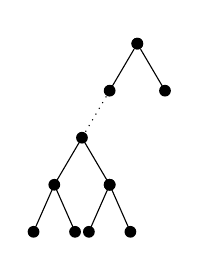
\begin{tikzpicture}[
baseline=-15, scale=1, every node/.style={dotA},
level distance=17pt,
sibling distance=20pt,
%level 1/.style={sibling distance=20pt},
%level 2/.style={sibling distance=20 pt},
%level 3/.style={sibling distance=20 pt},
level 4/.style={sibling distance=15 pt}
]
\node  [label=above:{}]  (root) {}
child {
	child 
	{
		edge from parent[draw=none]
%		edge from parent[dashed]
		child 
			{
			child  
			child
			}  
%		edge from parent[draw=none]
		child
			{
			child  
			child
			}  
	} 
	child
	{edge from parent[draw=none]}
}
child {};
\node at (root) {};
\node  at (root-1) {};
\node  at (root-2) {};
\path  (root-1) edge [ dotted, color=black] (root-1-1) ;
\node 
% [label={[label distance=-3pt]above:$\star$}, circle ,fill=white, draw=black,  inner sep=1.5pt
% ] 
at (root-1-1) {};
\node at (root-1-1-2) {};
\node at (root-1-1-1-2) {};
\node  at (root-1-1-1-1) {};
\node at (root-1-1-2-2) {};
\node  at (root-1-1-2-1) {};
\node 
at (root-1-1-1) {};
\node at (root-1-1-2) {};
\end{tikzpicture}
\caption{Type $\IV$.}
\end{subfigure}
\caption{Graphical representation of tree of Type $\I$, and examples of trees of Types $\II$--$\IV$. }
\label{FIG:types}
\end{figure}


\medskip

\noi (ii) From the definition of the multipliers in \eqref{wint0c}, note that the terms of Type $\III$ and $\IV$ do not have a restriction on the frequencies in the generation with parent $\pb(\star)$ and $\star$, respectively. This is a consequence of the calculation in \eqref{mul234}, where we see that they come from combining terms from $\mul_\bfrak(\TT)$ and $\mul_{\gfrak}(\TT)$, which come with $\ind_{A_{\star}^c} $ and $\ind_{A_\star}$, respectively.  


\end{remark}


Combining \eqref{w1}, Lemma~\ref{LEM:wbd}, and Lemma~\ref{LEM:wint}, we derive the modified normal form equation for the new variable $w$:
\begin{align}
\label{w2}
\dt w & =  \NN_1(\<1>;w) + \sum_{j=2}^\infty \sum_{\TT \in \Tr_j} \sum_{\l=2}^4  \NN_\l(\TT;w),
\end{align}
where the operators $\NN_\l$ are as in \eqref{wint0b}. 
We can regard $w$ as the interaction representation of another variable $z$, namely 
\begin{align}
\label{z0}
z(t) : = e^{-t\dx^3} w(t),
\end{align}
analogous to the relation between $u$ and $v$ in \eqref{inter}. In particular, $z$ satisfies the gauged KdV equation \eqref{rkdv}, whose exact form is given by
\begin{align}
\label{z1}
\dt z 
+ \dx^3 z
&
= 
e^{-t\dx^3}
\NN_1(\<1>;e^{t\partial_x^3}z) 
+ 
\sum_{j=2}^\infty \sum_{\TT \in \Tr_j} \sum_{\l=2}^4  
e^{-t\dx^3}
\NN_\l(\TT;e^{t\partial_x^3}z)
\\
&
=: 
\Ncal_1(\<1>;z) + \sum_{j=2}^\infty \sum_{\TT \in \Tr_j} \sum_{\l=2}^4  \Ncal_\l(\TT;z)
.
\end{align}



\subsection{Properties of the gauge transform and equivalence for smooth solutions}\label{sec:gauge_prop}
% \andreia{Do we also want to discuss equivalence between KdV and gauged equation here? That should only hold where the gauge is well-defined, I think }
In this section, we study the mapping properties of the gauge transform $\Gc$ (and its inverse) and prove that, for smooth solutions, \eqref{kdv} and \eqref{z1} are equivalent.

For the sake of clarity, let us recall the formal definition of the gauge transform \eqref{gauge} via its inverse: given
% In Section \ref{sec:multi}, we will use the Fourier restriction norm method to construct solutions for \eqref{z1}. Then, for sufficiently smooth initial data, we can recover solutions to  \eqref{kdv}, via the gauge transform $\Gc$ defined as follows: let 
$f \in \FL^{s,p}(\R)$,
\begin{align}\label{gauge1}
    \Gc^{-1}[f] 
    &
    = f + \Ft_x^{-1}\bigg( - \frac{1}{3} \int_{\xi=\xi_1+\xi_2} \ind_{A^c} \frac{1}{\xi_1\xi_2} \ft{f}(\xi_1) \ft{f}(\xi_2) d\xi_1 \bigg)\\&=f + e^{-t\dx^3} \D[e^{t\dx^3} f , e^{t\dx^3}f]
    \\
    &
     =: f + \DD [f, f]
    ,
\end{align}
for $A^c$ as in \eqref{A} and $\D$ as in \eqref{w} (see also \eqref{eq:D_intro}).
Note that $\Gc^{-1}$ and  $\Gc$ are time-independent. 

% Combining \eqref{z1}, \eqref{z0}, \eqref{w2}, 
% Lemma~\ref{LEM:wint}, Lemma~\ref{LEM:wbd}, \eqref{w1}, 
% \eqref{w}, 
% \eqref{NFE}, 
% Lemma~\ref{LEM:convNFE}, Proposition~\ref{PRO:NFE}, and \eqref{inter}, 
% we see that given $z$ a solution of \eqref{z1} with $z\vert_{t=0} = z_0$, then
% $
%     u = \Gc[z]
% $
% solves KdV \eqref{kdv}
% with $u\vert_{t=0} = z_0 + \DD[z_0,z_0]$. 
% The following result clarifies properties of the gauge transform $\Gc$ taking solutions $u$ to KdV \eqref{kdv} to solutions $z$ to \eqref{z1}, as well as its inverse given in \eqref{gauge1}.
 



\begin{lemma}\label{LEM:D}

Let $2<p\le \infty$ and consider the map  $\Gc^{-1}$ defined in \eqref{gauge1}.

\smallskip

\noi {\rm(i)}
Given $s>-\frac12 - \frac1p$, the map  $\Gc^{-1}$ is a continuous bijection on open balls $B_\dl \subset  \FL^{s,p}(\R)$ for $\dl>0$ sufficiently small. 
Consequently, the gauge transform $\Gc$ is a continuous map on $B_\dl$. 

\smallskip
\noi {\rm(ii)} The map $\Gc^{-1}$ is unbounded on $\FL^{s,p}(\R)$ for $s\le - \frac12 - \frac1p$. 

    
\end{lemma}


% \begin{remark}
%     \rm 
%     \color{red}
%     (ii) Comment on the ill-posedness result for $s<-\frac12 -\frac1p $ in Proposition~\ref{orop:ill_intro} being consistent with this result.
% \end{remark}

\begin{proof}

Considering $\Gc^{-1}$ in \eqref{gauge1}, we start by showing that $\Gc^{-1}$ is a small perturbation of the identity on $B_\dl \subset  \FL^{s, p}(\R)$, for $\dl>0$ sufficiently small. In particular, this follows once we show that $\DD$ is a contraction on this set. 
% We star by showing that
% \begin{equation}\label{eq:est_D}
% 		\|\D[z_{1},z_{2}]\|_{L^\infty_T \mathcal{F}L^{s,p}}
%         \les
% C\|z_{1}\|_{L^\infty_T \mathcal{F}L^{s,p}}\|z_{2}\|_{L^\infty_T \mathcal{F}L^{s,p}}. 
% \end{equation}

When $p=\infty$, recalling $A^c$ in \eqref{A}, we have
\begin{align}
\|\DD[z_{1},z_{2}]\|_{\mathcal{F}L^{s,\infty}}   
&
\les
\sup_\xi \jb{\xi}^s \int_{A^c} 
\frac{|\widehat{z}_{1}(\xi_{1})||\widehat{z}_{2}(\xi_{2})|}{\jap{\xi_{1}}\jap{\xi_{2}}} d\xi_{1} 
\notag
\\
&\les
\bigg( \sup_{\xi} \int_{|\xi_{1}|>1} \frac{1}{\jap{\xi_{1}}^{2s+2 - s\lor 0 }} d\xi_{1} 
\bigg) 
\|z_{1}\|_{\mathcal{F}L^{s,\infty}}\|z_{2}\|_{ \mathcal{F}L^{s,\infty}}
\notag
\\
& \les
\|z_{1}\|_{ \mathcal{F}L^{s,\infty}}
\|z_{2}\|_{ \mathcal{F}L^{s,\infty}}
\label{gaugeLinfty}
\end{align}
for $s>-\frac12$.
Similarly, for $p=2$, by duality and Cauchy-Schwarz inequality, we obtain
\begin{align}
\|\DD[z_{1},z_{2}]\|_{H^s}   
&
\les 
\sup_{\|z\|_{L^2} \le 1 }
	 \int_{\xi, (\xi_1,\xi_2)\in A^c} \frac{\jap{\xi}^s|\widehat{z}_{1}(\xi_{1})||\widehat{z}_{2}(\xi_{2})||\widehat{z}(\xi)|}{\jap{\xi_{1}}\jap{\xi_{2}}} d\xi_{1}d\xi 
     \notag
    \\
    & \les \sup_{\|z\|_{L^2 } \le 1}  \bigg( \sup_{\xi_{1}}  \int \ind_{A^c} \frac{\jap{\xi}^{2s}}{\jap{\xi_{1}}^{4s+4}}d\xi \bigg)^{\frac{1}{2}}
\|z_{1}\|_{H^s}\|z_{2}\|_{H^s}\|z\|_{L^2}
\notag
\\
&
\lesssim\  \|z_{1}\|_{H^s}\|z_{2}\|_{ H^s}, 
\label{gaugeL2}
\end{align}
given that $s>-1$. 
Then, from \eqref{gaugeLinfty} and \eqref{gaugeL2} together with interpolation, we have
\begin{equation}\label{eq:est_D}
		\|\DD[z_{1},z_{2}]\|_{ \mathcal{F}L^{s,p}}
        \les
\|z_{1}\|_{ \mathcal{F}L^{s,p}}\|z_{2}\|_{ \mathcal{F}L^{s,p}}. 
\end{equation}
for $2 \le p \le \infty$ and $s> -\frac12 - \frac1p$.
It follows from \eqref{eq:est_D} that $\DD$ is a contraction on $B_\dl \subset \FL^{s,p}(\R)$, for $\dl>0$ sufficiently small.




% Next, we establish time continuity of $\Gc$.
% Given $0\le t, t' \le T$ and $z \in C([0,T];\FL^{s, p}(\R))$, from \eqref{gauge} we have
% \begin{align}
%     \| \Gc_t(z) - \Gc_{t'}(z) \|_{\FL^{s, p}} 
%     &
%     \le 
%     \| z(t) - z(t') \|_{\FL^{s,p}}
%     +
%     \| \DD[z,z](t) - \DD[z,z](t') \|_{\FL^{s,p}}.
% \end{align}
% The convergence of the first contribution comes from the time continuity of $z$, while for the second, from \eqref{w}, we note that
% \begin{align}
%     | \DD[z,z](t) - \DD[z,z](t')| 
%     \les 
%     \int_{A^c} | e^{i(t - t' )\Psi(\cherryS)} - 1 | \frac{|\hat{z}_{1}(\xi_{1})||\hat{z}_{2}(\xi_{2})|}{\jap{\xi_{1}}\jap{\xi_{2}}} d\xi_{1}, 
% \end{align}
% where the convergence follows from dominated convergence theorem, due to the boundedness in \eqref{eq:est_D} and the convergence of the exponential factor.


\smallskip 

Lastly, we show the unboundedness of the map $\Gc^{-1}$ on $\FL^{s,p}(\R)$ for small $s$. Let $f \in \FL^{s, p}(\R)$ with 
\begin{align}
    \ft{f}(\xi) = \jb{\xi}^{-s-\frac1p}(\log \jap{\xi})^{-\frac12}. 
\end{align}
If $2 <p <\infty$, from \eqref{gauge1}, we have
\begin{align}
\| \DD[f,f] \|_{\FL^{s,p}}^p 
\ges 
\int_{|\xi|\le 1} \bigg| \int_{A^c} \frac{\ft{f}(\xi_1) \ft{f}(\xi_2) }{\xi_1\xi_2} d\xi_1 \bigg|^p d\xi
\sim \bigg( \int_{|\xi_1| \ge 1} \frac{1}{\jb{\xi_1}^{2s+2 + \frac2p  }\log\jap{\xi_1}} d\xi_1\bigg)^p , 
\end{align}
which diverges for $s\le-\frac12 - \frac1p$. For $p=\infty$, we have
\begin{align}
\| \DD[f,f]\|_{\FL^{s,\infty }}
\ges 
\sup_{|\xi| \le 1} 
\bigg| \int_{A^c} \frac{\ft{f}(\xi_1) \ft{f}(\xi_2) }{\xi_1\xi_2} d\xi_1 \bigg|
\sim 
\int_{|\xi_1| \ge 1 } \frac{1}{\jb{\xi_1}^{2s+2}\log\jap{\xi_1}} d\xi_1  ,
\end{align}
which also diverges, allowing us to conclude the unboundedness of $\DD$ on $\FL^{s, p}(\R)$, and thus that of $\Gc^{-1}$. 
\qedhere 

\end{proof}

We can now prove that, under the gauge transform $\Gc$, \eqref{kdv} and \eqref{rkdv} (more specifically, \eqref{z1}) are equivalent for smooth solutions.


\begin{proposition}\label{prop:equivalencia}
Fix $s\gg 1$, $2\le p < \infty$, and $T>0$. There exists $\delta>0$ such that, given $u_0\in \FL^{s,p}(\R)$ with $\|u_0\|_{\FL^{s,p}(\R)}<\delta$, the following are equivalent:

\smallskip
\noi{\rm(i)} $u\in C([0,T], \FL^{s,p}(\R))$ is a strong integral solution to  \eqref{kdv} with initial data $u_0$.

\smallskip
\noi{\rm(ii)} $v=e^{t\dx^3}u\in C([0,T], \FL^{s,p}(\R))$ is a strong integral solution of \eqref{NFE} (with absolute summability of the nonlinear terms) for the initial data $u_0$.

\smallskip
\noi{\rm(iii)} $z=\Gc^{-1}[u]\in C([0,T], \FL^{s,p}(\R))$ is a strong integral solution of \eqref{z1} (with absolute summability of the nonlinear terms) for the initial data  $z_0=\Gc^{-1}[u_0]$.

\end{proposition}

\begin{remark}
    In the case $p=\infty$, an analogous statement holds, where one must replace the time-continuity of $u$ and $z$ with that of the interaction representations (see Remark \ref{remark:Linfty_continuity}).
\end{remark}

\begin{proof}
    \textit{Step 1. \rm(i)$\Rightarrow$\rm(ii).} The proof of this implication is tantamount to the formalization of the infinite normal form reduction, which relies on four technical assumptions (see also the discussion in \cite[Section 4]{KOY20}): the differentiation-by-parts in time; the dominated convergence theorem to exchange time derivatives and frequency integrals; the summability of the terms $\NN(\TT;v)$ and $\BB(\TT;v)$; the convergence of the remainders $\MM(\TT;v)$ to zero (in some topology).
	
	Concerning the two first assumptions, this is guaranteed by the decay of both $v$ and $v_t$ (as $s\gg 1$) and the fact that, for $\xi$ fixed, $v$ is $C^1$ in the time variable.
	To verify the third condition, we observe that, if $\TT\in \Tr_{j}$, $j\ge 2$, then
    \begin{equation}\label{eq:estimativa_mul}
        |\mulB(\TT)| + |\mul(\TT)|\le C^j,
    \end{equation}
    for some $C>0$.  As such, 
	\begin{align*}
	&\left\|\int_0^t(\NN(\TT;v)+\BB(\TT;v))(t')dt\right\|_{\mathcal{F}L^{s,p}(\R)}\\\lesssim\ & (1+T)C^j\sup_\xi \left( \int_{\xi=\sum_{\bul\in\TT^\infty}\xi_\bul} \left(\jap{\xi}^{s}\prod_{{\bul\in \TT^\infty}} \frac{1}{\jap{\xi_\bul}^{s}}\right)^{p'} d\vec{\xi} \right)^{\frac{1}{p'}}\|u\|_{L
    ^\infty((0,T),\mathcal{F}L^{s,p}(\R))}^{j+1}\\\lesssim\ & (C(T,s,p)\delta)^j,
	\end{align*}
    where we used the fact that $|\xi|\le (j+1)\max_{\bul\in\TT^\infty}|\xi_\bul|$.
    
    If $\TT\in \Tr_1$, that is, $\TT=\<1>$, then
        \begin{equation}\label{eq:estimativa_mul2}
        |\mulB(\<1>)|\le 1,\quad |\mul(\<1>)|\frac{\jap{\xi}}{\jap{\xi_1}\jap{\xi_2}}\le C,
    \end{equation}
since $\mul(\<1>)$ includes the restriction to the region $|\xi_1|\simeq |\xi_2|\gtrsim |\xi|$. In particular,
\begin{align*}
	&\left\|\int_0^t(\NN(\<1>;v) + \BB(\<1>;v))(t')dt'\right\|_{\mathcal{F}L^{s,p}(\R)}\\\lesssim\ & (1+T)\sup_\xi \left( \int_{\xi=\xi_1+\xi_2} \left(\frac{\jap{\xi}^{s-1}}{\jap{\xi_1}^{s-1}\jap{\xi_2}^{s-1}}\right)^{p'} d\xi_1 \right)^{\frac{1}{p'}}\|u\|_{L
    ^\infty((0,T),\mathcal{F}L^{s,p}(\R))}^{2}\lesssim\  (C(T,s,p)\delta)^2,
	\end{align*}
In particular,
\begin{equation}
    \sum_{j\ge 1}\sum_{\TT\in\Tr_j}\left\|\int_0^t(\NN(\TT;v)+\BB(\TT;v))(t')dt\right\|_{\mathcal{F}L^{s,p}(\R)} \lesssim \sum_{j\ge 1}\frac{(2j)!}{j!(j+1)!}(C(T,s,p)\delta)^j <\infty,
\end{equation}
for $\delta=\delta(T,s,p)$ small, thus proving the summability of $\NN$ and $\BB$. 

It remains to prove the decay of the remainder terms $\MM(\TT)$, $\TT\in \Tr_j$ as $j\to \infty$. Since
$$
|\Psi(\star)|\le C^j\max_{\bul\in \TT^\infty} |\xi_\bul|^3,
$$
it follows from \eqref{NFE1a}, \eqref{eq:estimativa_mul} and \eqref{eq:estimativa_mul2} that
\begin{align}
    &\left\|\int_0^t\MM(\TT;v)(t')dt'\right\|_{\FL^{s,p}(\R)} \\\lesssim &\ (1+T)C^j\sup_\xi \left( \int_{\xi=\sum_{\bul\in\TT^\infty}\xi_\bul} \left(\jap{\xi}^{s}\left(\max_{\bul\in\TT^\infty}|\xi_\bul|^3\right)\prod_{{\bul\in \TT^\infty}} \frac{1}{\jap{\xi_\bul}^{s}}\right)^{p'} d\vec{\xi} \right)^{\frac{1}{p'}}\delta^{j+1}\\\lesssim\ &(C(T,s,p)\delta)^j,
\end{align}
Therefore
$$
\sum_{\TT\in \Tr_j}\left\|\int_0^t\MM(\TT;v)(t')dt'\right\|_{\FL^{s,p}(\R)} \lesssim \frac{(2j)!}{j!(j+1)!}(C(T,s,p)\delta)^j \to 0\quad \mbox{as }j\to\infty.
$$

\smallskip
\noi\textit{Step 2.} (ii)$\Rightarrow$(i). Taking into account Step 1, it suffices to prove the uniqueness of solution for \eqref{NFE}. Given two solutions $v, v'\in C([0,T], \FL^{s,p}(\R))$, the same computations from Step 1 yield
\begin{align*}
    &\|v(t)-v'(t)\|_{\FL^{s,p}(\R)}\\\lesssim\ & \sum_{j\ge 1} \sum_{\TT\in\Tr_j} \left\|\int_0^t((\NN(\TT;v)-\NN(\TT;v'))+(\BB(\TT;v)-\BB(\TT;v')))(t')dt\right\|_{\mathcal{F}L^{s,p}(\R)}\\\lesssim \ & \sum_{j\ge 1} \frac{(2j)!}{j!(j+1)!} (C(T,s,p)\delta)^{j-1}\|v-v'\|_{L^\infty((0,T),\FL^{s,p}(\R))} \le \frac{1}{2}\|v-v'\|_{L^\infty((0,T),\FL^{s,p}(\R))} 
\end{align*}
and thus $v=v'$.

\smallskip
\noi\textit{Step 3.} (ii)$\Leftrightarrow$(iii). This is a direct consequence of Section \ref{SUBSEC:gauge}, the invertibility properties of $\Gc$ and the fact that the cancellations observed in Lemmas \ref{LEM:wbd} and \ref{LEM:wint} are term-by-term cancellations.
\end{proof}
% \simao{PAREI AQUI, AMANHÃ DE MANHÃ COMPLETO. FORÇA VASCO!}

%     fix $t>0$ and observe that, for either $\NN, \B$ or $\MM$, the corresponding multiplier (see \eqref{NFE1a}) is controlled by 
% 	$$\max_{\bul\in \TT^\infty}|\xi_\bul|.
% 	$$ As such, given a tree $\TT\in \Tr_N$,
% 	\begin{align*}
% 	&\||\NN(\TT)(t)| + |\B(\TT)(t)| + |\MM(\TT)|(t)\|_{\mathcal{F}L^{s-3,p}(\R)}\\\lesssim\ & (1+T)\sup_\xi\sum_{\ast \in \TT^0} \left( \int_{\xi=\sum_{\bul\in\TT^\infty}\xi_\bul} \left({\jap{\xi}^{s-3}\max_{\bul\in \TT^\infty}|\xi_\bul|}\prod_{{\bul\in \TT^\infty}} \frac{1}{\jap{\xi_\bul}^{s}}\right)^{p'} d\vec{\xi} \right)^{\frac{1}{p'}}\|u\|_{\mathcal{F}L^{s,p}(\R)}^{N+1}\\\lesssim\ & C(T,s,p)^N\|u_0\|_{\mathcal{F}L^{s,p}(\R)}^{N+1},
% 	\end{align*}
% 	where the factor $T$ comes from bounding in absolute value the integration in time. In particular, summing over $\TT\in \Tr_N$,
% \begin{align*}
% 		\sum_{\TT\in \Tr_N} \||\NN(\TT)(t)| + |\B(\TT)(t)| + |\MM(\TT)|(t)\|_{\mathcal{F}L^{s-3,p}(\R)} &\lesssim |\Tr_N|C(T,s,p)^N\|u_0\|_{\mathcal{F}L^{s,p}(\R)}^{N+1}\\&\lesssim \frac{(2N)!}{N!(N+1)!}C(T,s,p)^N\|u_0\|_{\mathcal{F}L^{s,p}(\R)}^{N+1},
% \end{align*}
% 	which converges exponentially to 0 as $N\to \infty$ if $\|u_0\|_{\mathcal{F}L^{s,p}(\R)}$ is sufficiently small.
% \end{proof}


% The following result shows the convergence to zero of the error terms  $\MM(\TT; v)(t)$ in \eqref{NFE1}  as $J\to\infty$, for smooth solutions to \eqref{kdv}. 


% % \andreia{Need to discuss this further and also where it should come in the text}


% \begin{lemma}
% Let $T>0$, $2 \le p \le \infty$, and $v \in L^\infty([0,T];  \bigcap_{s\ge0} \FL^{s,p}(\R) ) $ with $\| v\|_{L^\infty_T \FL^{s, p}_x} \le R$ and $0<R \ll 1$ sufficiently small. 
% Then, for $(2s-1)p'>1$, we have
% \begin{align}
% \sup_{|t| \le T } \bigg\| \sum_{\TT\in \Tr_J} \MM(\TT; v ) (t) \bigg\|_{ \FL^{s, p} } \to 0, 
% \end{align}
% as $J\to\infty$.
% Consequently, given 

% \end{lemma}


% {


% \begin{proof}

% Let $J\ge 2$, $\TT\in \Tr_J$, and $\MM$ as in \eqref{NFE1a}. Then, fixing $| t| \le T$, from \eqref{NFE0b} and H\"older's inequality, we have
% \begin{align}
%  &
%  \| \MM(\TT; v)(t) \|_{\FL^{s, p}}
%  \\
%  &
%  \le C 
%  T \sup_{|t| \le T}
%  \bigg\| 
%  \int_{\G(\TT)} \jb{\xi}^{s} \Psi(\TT) \bigg(\prod_{\bul \in \TT^0} \ind_{A_\bul^c} K_\bul \bigg) \prod_{\bul\in\TT^\infty} \ft{v}_\bul d \vec\xi  \, 
%  \bigg\|_{L^p_\xi }
%  \\
%  &
%  \le
%  C^J
%  T \| v\|^{J+1}_{L^\infty_T \FL^{s, p}_x} 
%  \sup_\xi \bigg\{
%  \int_{\G(\TT)} \jb{\xi}^{sp'} \bigg(
%  \prod_{\bul\in\TT^\infty\setminus\{\star1, \star2\}} \frac{1}{\jb{\xi_\bul}^{(s+1)p'}}
%  \bigg)
%  \frac{1}{\jb{\xi_{\star1}}^{(2s+2-3)p'}}
%  d\vec\xi \, 
%  \bigg\}^{\frac{1}{p'}}
%  \\
%  &
%  \le C^J T \| v\|^{J+1}_{L^\infty_T \FL^{s, p}_x} 
%  \sup_\xi 
%  \bigg( \prod_{\bul\in \TT^\infty\setminus\{\star1,\star2\}}\frac{1}{\jb{\xi_\bul}^{(s+1 - \frac{s}{J-1})p' + }} d\xi_\bul  \bigg)^{\frac{1}{p'}} 
%  \bigg( 
%  \int
%  \frac{1}{\jb{\xi_{\star1}}^{(2s -1 )p' -}} d\xi_{\star1}
%  \bigg)^{\frac{1}{p'}}
%  \\
%  &
%  \le C^J T \| v\|^{J+1}_{L^\infty_T \FL^{s, p}_x} 
% \end{align}
% given that $(2s-1)p' > 1$,
% % 
% where we used that $|\Psi(\TT)| \le J |\Psi(\star)| \les |\xi_{\star1}|^3
% $ for some $\star \in \TT^{0,\ff}$, $\prod_{\bul\in \TT^0} |K_\bul| \le C^J \prod_{\bul\in\TT^\infty} \jb{\xi_\bul}^{-\frac12}$, and $|\xi| \le C^J |\xi_{\bul}|$ for all $\bul\in\TT^\infty$, due to the restriction to $\bigcap_{\bul\in \TT^0} A_\bul^c$ defined in \eqref{defA}. 
% Note that $C$ above is independent of $T$ and $v$. Summing in $\TT\in \Tr_J$ with \eqref{eq:catalan}, we obtain
% \begin{align}
%   \sup_{|t| \le T }  \bigg\| \sum_{\TT\in\Tr_J} \MM(\TT; v ) (t) \bigg\|_{\FL^{s, p}} 
%   &
%   \le C^J \frac{(2J)!}{(J+1)! J!} T \|v\|^{J+1}_{L^\infty_T \FL^{s,p}_x} 
%   \le 
%   C^J \frac{(2J)!}{(J+1)! J!} T R^{J+1} \to 0, 
% \end{align}
% as $J\to\infty$ for $R=R(T)>0$ sufficiently small. 


% \andreia{Add comment that the normal form equation holds for smooth solutions, then. 
% This should follow saying that any equation satisfying the Duhamel formulation also satisfies the normal form equation (in limit form), for sufficiently smooth  solutions. 

% Looking at $J$-th iterate, we can use the multilinear estimates to make sense of all terms in some topology, and this lemma says we can take the limit. 

% Looking at the difference between the solution and the iterate at $J$ without the error term, the multilinear estimates say that there is a limit as $J\to\infty$ due to summability. But we also know that this limit should be 0 due to convergence.

% Since for fixed $J$, all the steps are justified for smooth solutions (since we do derivation by parts and products, which should be okay for $s$ large enough) 
% }


% \color{blue}


% \andreia{CHECK }


% 	The formal procedure that leads to \eqref{NFE} relies on four technical assumptions (see also the discussion in \cite[PÁGINA]{KOY}): the integration-by-parts in time; Fubini's theorem to exchange time and frequency integrals; the summability of the terms $\NN(\TT)$ and $\B(\TT)$; the convergence of the remainders $\mathcal{M}(\TT)$ to zero (in some topology).
	
% 	Concerning the two first assumptions, this is guaranteed by the (infinite) decay of both $v$ and $v_t$ and the fact that, for $\xi$ fixed, $v$ is $C^1$ in the time variable.
	
% 	To verify the last two conditions, let us fix $t>0$ and observe that, for either $\NN, \B$ or $\MM$, the corresponding multiplier (see \eqref{NFE1a}) is controlled by 
% 	$$\max_{\bul\in \TT^\infty}|\xi_\bul|.
% 	$$ As such, given a tree $\TT\in \Tr_N$,
% 	\begin{align*}
% 	&\||\NN(\TT)(t)| + |\B(\TT)(t)| + |\MM(\TT)|(t)\|_{\mathcal{F}L^{s-3,p}(\R)}\\\lesssim\ & (1+T)\sup_\xi\sum_{\ast \in \TT^0} \left( \int_{\xi=\sum_{\bul\in\TT^\infty}\xi_\bul} \left({\jap{\xi}^{s-3}\max_{\bul\in \TT^\infty}|\xi_\bul|}\prod_{{\bul\in \TT^\infty}} \frac{1}{\jap{\xi_\bul}^{s}}\right)^{p'} d\vec{\xi} \right)^{\frac{1}{p'}}\|u\|_{\mathcal{F}L^{s,p}(\R)}^{N+1}\\\lesssim\ & C(T,s,p)^N\|u_0\|_{\mathcal{F}L^{s,p}(\R)}^{N+1},
% 	\end{align*}
% 	where the factor $T$ comes from bounding in absolute value the integration in time. In particular, summing over $\TT\in \Tr_N$,
% \begin{align*}
% 		\sum_{\TT\in \Tr_N} \||\NN(\TT)(t)| + |\B(\TT)(t)| + |\MM(\TT)|(t)\|_{\mathcal{F}L^{s-3,p}(\R)} &\lesssim |\Tr_N|C(T,s,p)^N\|u_0\|_{\mathcal{F}L^{s,p}(\R)}^{N+1}\\&\lesssim \frac{(2N)!}{N!(N+1)!}C(T,s,p)^N\|u_0\|_{\mathcal{F}L^{s,p}(\R)}^{N+1},
% \end{align*}
% 	which converges exponentially to 0 as $N\to \infty$ if $\|u_0\|_{\mathcal{F}L^{s,p}(\R)}$ is sufficiently small.
% \end{proof}






	\section{Functional framework}\label{sec:functional}
	
	In this section, we introduce the function spaces over which the solution to \eqref{rkdv} will be built and prove linear estimates associated with the Duhamel integral formulation (Section \ref{sec:fourier_restr}). The crux of the  construction of the solution are specific multilinear estimates, which we reduce to  frequency-restricted estimates (Section \ref{sec:fre}).
	
	
	\subsection{Fourier restriction spaces}\label{sec:fourier_restr}
	
	We first recall the Fourier restriction norm spaces $X^{s,b}_{p,q}$, first introduced by Bourgain \cite{bourg1, bourg2} and Klainerman-Machedon in \cite{KlainermanMachedon} and adapted to the Fourier-Lebesgue setting in \cite{Grunrock_mkdv, HerrGrunrock_FL}.
	
		
		
		Let $s,b\in \R$ and $1\le p,q \le \infty$. We consider the Fourier restriction spaces $X^{s,b}_{p,q}$ defined through the norm
		% \begin{align}\label{defi:bourg_space}
		% 	X^{s,b}_{p,q} =\{ u\in \mathcal{S}(\R\times \R) : \|u\|_{X^{s,b}_{p,q}}<\infty\},
		% \end{align}
		% where the norm is given by
		\begin{equation}\label{Xsb}
			\| u \|_{X^{s,b}_{p,q}} := \| \jap{\xi}^s \jap{\tau-\xi^3}^b \F_{t,x}(u) (\tau, \xi) \|_{L^p_\xi L^q_\tau}
            =
            \| \jb{\xi}^s \jb{\tau}^b \F_{t,x}(e^{t \dx^3} u ) (\tau, \xi) \|_{L^p_\xi L^q_\tau}. 
		\end{equation}
When $p=q$, we may also abbreviate $X^{s,b}_{p,q}$ as $X^{s,b}_p$. 
		The case $p=q=2$ corresponds to the classic Fourier restriction spaces (\cite{bourg1, bourg2}. 
        Given $T>0$, we also recall the time-localized space $X^{s, b}_{p,q} (0,T)$ defined via the following norm
        \begin{align}
            \| u\|_{X^{s, b}_{p,q}(0,T)} : = \inf 
            \big\{ 
            \| v\|_{X^{s, b}_{p,q}} : \ v\in X^{s,b}_{p,q}, \ v\vert_{[0,T]} = u 
            \big\}, 
        \end{align}
        where the infimum is taken over all extensions of $u$. See \cite[Chapter 2.6]{tao_book}, \cite[Chapter 7.4]{linares_ponce_book}), and  \cite{HerrGrunrock_FL} for proofs. 
        Let  $\psi\in C_c^\infty(\R)$ be a smooth cut-off function with $\psi\equiv 1$ over $[-1,1]$ and $\psi\equiv 0$ on $\R\setminus [-2,2]$, and given $T>0$, we set $\psi_T(t)=\psi(t/T)$.
        
        
        
\begin{lemma}
\label{lem:linear_estimates_qfinite}
			Let $s\in\R$, $2\le p <\infty$, and $b,b'\in\R$ with $b > \frac{1}{p'}$ and $-\frac1p<b' \le 0 \le b \le 1+b'$. 

            % \smallskip
			\noi{\rm(i)} The following embedding holds: $X^{s,b}_{p} \hookrightarrow C(\R;\FL^{s,p}(\R))$. 
            
			\smallskip
			\noi{\rm(ii)} For all $f \in \FL^{s,p}(\R)$ and $F \in X^{s, b'}_p$, we have
			\begin{align}
				\label{lin1_gh}
				\| \psi e^{-t\dx^3} f \|_{X^{s,b}_{p}} &\les \| f \|_{\FL^{s,p}}, 
                \\
				\bigg\| \psi_T (t) \int_0^t e^{-(t-t')\dx^3 } F(t') \, dt' \bigg\|_{X^{s,b}_{p} } 
                &
                \les T^{1+b'-b} \| F \|_{X^{s,b'}_{p}}.
                \label{lin2a_gh}
			\end{align}
			
		\end{lemma}

        
		It is important to stress that, in the above result, the case $p=\infty$ is out-of-reach. Nevertheless, this delicate case can still be addressed by exploiting a different integrability exponent for the time-frequency variable, as the next lemma shows. For a similar result, see \cite[Section 7]{CC24}. 
		
		\begin{lemma}\label{lem:linear_estimates}
			Let $s\in\R$, $b,\wt b, b', \wt b'\in\R$ satisfying
            \begin{align}
                \label{bs}
                -1 < b' \le 0 \le b < 1 + b'
                \quad 
                \text{and} 
                \quad 
                -1 < \wt b' \le 0 \le \wt b < 1 + \wt b', 
            \end{align}
        and $\wt u(t) := e^{t\dx^3 } u(t)$. 
        
        % \smallskip
            \noi 
			{\rm(i)} For $b>0$,  given $u\in X^{s,b}_{\infty,1}$, we have $\wt{u}\in C(\R;\FL^{s,\infty}(\R))$ with
			\begin{equation}\label{lin}
				\|\wt{u}\|_{L^\infty_t\FL^{s, \infty}_x}\lesssim \|u\|_{X^{s,b}_{\infty,1}}, 
			\end{equation}
			and the following embedding holds
			\noi
			\begin{align}
				X^{s,b}_{\infty, 1} &
                \embeds C(\R; \FL_{\mathrm{loc}}^{s,\infty}(\R))\cap L^\infty(\R; \FL^{s,\infty}(\R)), 
			\end{align}
            where $f \in \FL^{s, \infty}_{\mathrm{loc}}(\R)$ if for any compact set $K\subset \R$, $\P_K f \in \FL^{s, \infty}(\R)$, with $\P_K$  denoting the Dirichlet projection onto spatial frequencies $ \xi \in K$.


			
			\smallskip
			
			\noi {\rm(ii)} 
            For $ 1 \le q \le \infty$, we have 
			\begin{align}
				\label{lin1}
				\| \psi e^{-t\dx^3} f \|_{X^{s,b}_{\infty,q}} \les \| f \|_{\FL^{s,\infty}}.
			\end{align}
			
			% \smallskip
			
			\noi{\rm(iii)} Moreover, if $2 - b + \wt b' \ge0$, the following inhomogeneous estimates hold
            
			\noi
			\begin{align}
				\label{lin2a}
				\bigg\| \psi_T (t) \int_0^t e^{-(t-t')\dx^3 } F(t') \, dt' \bigg\|_{X^{s,\wt{b}}_{\infty,1} } & \les T^{1+\wt{b}'-\wt{b}} \| F \|_{X^{s,\wt{b}'}_{\infty,1}}
                ,
            \\
				\label{lin2b}
				\bigg\| \psi_T (t) \int_0^t e^{-(t-t')\dx^3} F(t') \, dt' \bigg\|_{X^{s,b}_{\infty, \infty} } 
                &
                \les T^{1+b'-b} \| F\|_{X^{s, b'}_{\infty, \infty}} + T^{2+\wt{b}' -b} \|F\|_{X^{s, \wt{b}'}_{\infty, 1}}.
			\end{align}
			
			
			
		\end{lemma}
		
		\begin{proof}
			
			We begin with (i). Given $u\in X^{s,b}_{\infty,1}$,
			$$
            \Ft_x(\wt u)(t,\xi) = \int e^{it\tau}\ft{u}(\tau+\xi^3,\xi)d\tau, 
			$$ 
            from which we have
$$\| u(t)\|_{\FL^{s,\infty}_x} = \|\wt{u}(t)\|_{\FL^{s,\infty}_x} \lesssim \|\jap{\xi}^s\ft {u}\|_{L^\infty_\xi L^1_\tau} \les \|u\|_{X^{s,b}_{\infty,1}}, 
			$$
            for $b\ge 0$. 
			Moreover, given $t,t'\in\R$,
			\begin{align*}
				\|\wt{u}(t)-\wt{u}(t')\|_{\FL_x^{s,\infty}} &\lesssim \bigg\|\int \frac{e^{it\tau}-e^{it'\tau}}{\jap{\tau}^b}\jap{\xi}^s\jap{\tau}^b\ft{u}(\tau+\xi^3,\xi)d\tau\bigg\|_{L^\infty_\xi}\\&\lesssim \sup_{\tau} \bigg| \frac{e^{it\tau}-e^{it'\tau}}{\jap{\tau}^b}\bigg| \|u\|_{X^{s,b}_{\infty,1}} \to 0 \quad \mbox{as }t\to t',
			\end{align*}
            for any $b>0$, 
			and thus $\wt{u}\in C_b(\R;\FL^{s,\infty}(\R))$. Finally, considering a compact set $K\subset \R$, we have
			\begin{align*}
				\| \P_K [u(t)-u(t')]\|_{\mathcal{F}L^{s,\infty}_x} 
                &
                \lesssim \|\wt{u}(t)-\wt{u}(t')\|_{\FL^{s,\infty}_x} 
                + \|\jb{\xi}^s (1-e^{-i(t-t')\xi^3})\ft{u}(t')\|_{\FL^{\infty}_x (K) } \\&\lesssim \|\wt{u}(t)-\wt{u}(t')\|_{L^{s,\infty}_\xi} + \sup_{\xi\in K}\big|1 -e^{-i (t-t')\xi^3}\big| \| u \|_{X^{s,b}_{\infty,1}} \to 0\quad \mbox{as }t\to t', 
			\end{align*}
            from the earlier convergence 
			which implies that $u\in C(\R;\mathcal{F}L^{s,\infty}_{\mathrm{loc}}(\R))$. 


            The proof of (ii) is a direct consequence of
			$$
			\|\psi e^{-t\partial_x^3}f\|_{X^{s,b}_{\infty,q}} = \|\jap{\xi}^s\jap{\tau}^b\ft{\psi}(\tau)\ft{f}(\xi)\|_{L^\infty_\xi L^q_\tau} \lesssim \|\psi\|_{\FL^{b,q}} \|f\|_{\FL^{s,\infty}}.
			$$

            
            
            
			\smallskip
			
			We now move to the proof of (iii), where we proceed as in the proof of \cite[Lemma~2]{Grunrock_mkdv}.
            Note that \eqref{lin2a}-\eqref{lin2b} is equivalent to 
            \begin{align}
                \bigg\| \psi_T (t) \int_0^t G(t') \, dt' \bigg\|_{\FL^{s, p}_x \FL^{b_1, q_1 }_t }
                \les T^{1+ q_2 - q_1} \| G \|_{\FL^{s, p}_x \FL^{b_2 , q_2}_t }, 
            \end{align}
            for $G = e^{t\partial_x^3} F$, for suitable choices of the parameters. Thus, we start by expanding the quantity on the l.h.s.:
			\begin{equation}
				\psi_T(t)\int_0^t G(s) ds =  c \psi_T (t)\int \frac{e^{it\eta}-1}{i\eta } (\mathcal{F}_t G )(\eta,x) d\eta = \I + \II + \III,
				\label{lin3a}
			\end{equation}
			where
			\begin{equation}
				\label{lin3}
				\begin{aligned}
					\I & :=c\psi_T(t)\sum_{k= 1}^\infty \frac{t^k}{k!}\int_{|\eta| T \le 1} (i\eta)^{k-1} (\mathcal{F}_t G )(\eta,x) d\eta, \\
					\II& :=-c\psi_T (t)\int_{|\eta|T \ge 1} (i\eta)^{-1} (\mathcal{F}_t G )(\eta,x) d\eta , \\
					\III & :=c\psi_T (t)\int_{|\eta| T  \ge 1} e^{it\eta}(i\eta)^{-1} (\mathcal{F}_t G )(\eta,x) d\eta,
				\end{aligned}
			\end{equation}
			for some constant $c\in\R$.
			%
			%
			%
            
            
            The space-time Fourier transform of $\I$ in \eqref{lin3} satisfies
			\begin{equation}
				|(\mathcal{F}_{t,x}\I)(\tau, \xi)| \les \sum_{k= 1}^\infty \frac{|\widehat{t^k\psi_T}(\tau)|}{k!} \int_{|\tau|T  \le 1} |\eta|^{k-1} |\ft{G }(\eta,\xi)| d\eta, 
				\label{lin4a}
			\end{equation}
            which combined with H\"older's inequality gives
			\begin{align}
					\| \jap{\xi}^s \jap{\tau}^b \F_{t,x} \I \|_{L^\infty_\xi L^\infty_\tau} & \les \sum_{k=1}^\infty \frac{1}{k!} \| \jap{\tau}^b\ft{t^k \psi_T} (\tau) \|_{L^\infty_\tau} \bigg( \int_{|\eta|T \le 1} |\eta|^{k-1} \jap{\eta}^{-b'} d\eta \bigg) \| \jap{\xi}^s \jap{\eta}^{b'} \ft{G}(\eta, \xi) \|_{L^\infty_\xi L^\infty_\eta} \\
					& \les_\psi T^{1+ b' -b} \| G \|_{\FL^{s, \infty}_x \FL^{b', \infty}_t },
				\label{lin4b}
			\end{align}
			\noi
			since $k-1-b' \ge0$ for $b' \le 0$.
			% \begin{equation}
			% 	k-1-b' \ge 0 .
			% 	\label{lin4bb}
			% \end{equation}
			Similarly, since $\tilde{b}'\le 0$,
			\begin{equation}
				\begin{aligned}
					\| \jap{\xi}^s \jap{\tau}^{\tilde{b}} \F_{t,x} \I \|_{L^\infty_\xi L^1_\tau} & \les \sum_{k=1}^\infty \frac{1}{k!} \| \jap{\tau}^{\wt{b}}\ft{t^k \psi_T} (\tau) \|_{L^1_\tau} \bigg( \sup_{|\eta|T \le 1} |\eta|^{k-1} \jap{\eta}^{-\wt{b}'}  \bigg) \| \jap{\xi}^s \jap{\eta}^{\wt{b}'} \ft{G}(\eta, \xi) \|_{L^\infty_\xi L^1_\eta} \\
					& \les_\psi T^{1+ \wt{b}' -\wt{b}} \| G \|_{\FL^{s, \infty}_x \FL^{\wt b ', 1}_t},
				\end{aligned}
				\label{lin4c}
			\end{equation}
			

			
			For $\II$ in \eqref{lin3}, by H\"older's inequality, we have
			\begin{equation}
				\begin{aligned}
					\| \jap{\xi}^s \jap{\tau}^b \F_{t,x} \II \|_{L^\infty_\xi L^\infty_\tau} & \les \bigg\| \jap{\tau}^b \ft{\psi}_T(\tau) \int_{|\eta|T >1} \jap{\xi}^s |\eta|^{-1} | \ft{G}(\eta, \xi)| d\eta \bigg\|_{L^\infty_\xi L^\infty_\tau} \\
					& \les \| \jap{\tau}^b \ft{\psi_T}(\tau) \|_{L^\infty_\tau} \Big( \sup_{|\eta| T >1} |\eta|^{-1} \jap{\eta}^{-\wt{b}'} \Big) \| \jap{\xi}^s \jap{\eta}^{\wt{b}'} \ft{G}(\eta, \xi) \|_{L^\infty_\xi L^1_\eta} \\
					& \les_\psi T^{2 + \wt{b}' - b} \| G  \|_{\FL^{s, \infty}_x \FL^{\wt b ', 1}_t},
				\end{aligned}
				\label{lin5a}
			\end{equation}
			given that $\wt b ' >-1$. 
			Analogously,
			\begin{equation}
				\begin{aligned}
					\| \jap{\xi}^s \jap{\tau}^{\wt{b}} \F_{t,x} \II \|_{L^\infty_\xi L^1_\tau} & \les \bigg\| \jap{\tau}^{\wt{b}} \ft{\psi}_T(\tau) \int_{|\eta|T >1} \jap{\xi}^s |\eta|^{-1} | \ft{G}(\eta, \xi)| d\eta \bigg\|_{L^\infty_\xi L^\infty_\tau} \\
					& \les \| \jap{\tau}^{\wt{b}} \ft{\psi_T}(\tau) \|_{L^1_\tau} \Big( \sup_{|\eta| T >1} |\eta|^{-1} \jap{\eta}^{-\wt{b}'} \Big) \| G  \|_{\FL^{s, \infty}_x \FL^{\wt b', 1}_t}
                    \\
						& \les_\psi T^{1 + \wt{b}' - \wt{b}} \| G \|_{\FL^{s, \infty}_x \FL^{\wt b ', 1}_t}, 
				\end{aligned}
				\label{lin5c}
			\end{equation}
            for $\wt b'>-1$. 
			
			
			
			Lastly, for $\III$, from \eqref{lin3} and H\"older's inequality, we have
			\begin{equation}
				\begin{aligned}
					\| \jap{\xi}^s \jap{\tau}^b \F_{t,x} \III \|_{L^\infty_\xi L^\infty_\tau} & \les \bigg\| \jap{\xi}^s \int_{|\eta|T >1} \jap{\eta}^b |\eta|^{-1} |\ft{G}(\eta, \xi) \ft{\psi}_T(\tau-\eta) | d\eta \bigg\|_{L^\infty_\xi L^\infty_\tau} \\
					& \quad + \bigg\| \jap{\xi}^s \int_{|\eta|T >1}  |\eta|^{-1} |\ft{G}(\eta, \xi)| \jap{\tau - \eta}^b | \ft{\psi}_T(\tau-\eta) | d\eta \bigg\|_{L^\infty_\xi L^\infty_\tau} \\
					& \les \Big( \sup_{|\eta|T>1} \jap{\eta}^{b-b'} |\eta|^{-1} \Big) \| \jap{\xi}^s \jap{\eta}^{b'} \ft{G}(\eta, \xi) \|_{L^\infty_\xi L^\infty_\eta} \| \ft{\psi}_T \|_{L^1_\tau} \\
					& \quad + \Big( \sup_{|\eta|T>1} |\eta|^{-1} \jap{\eta }^{-b'} \Big)  \| \jap{\xi}^s \jap{\eta}^{b'} \ft{G}(\eta, \xi) \|_{L^\infty_\xi L^\infty_\eta} \| \jap{\tau}^{b} \ft{\psi}_T \|_{L^1_\tau } \\
					& \les T^{1+b'-b} \| G\|_{\FL^{s, \infty}_x \FL^{b', \infty}_t}
				\end{aligned}
				\label{lin6a}
			\end{equation}
			given that $b-b' < 1 $ and $b'>-1$.
			Similarly, 
			\begin{equation}
				\begin{aligned}
					\| \jap{\xi}^s \jap{\tau}^{\wt{b}} \F_{t,x} \III \|_{L^\infty_\xi L^1_\tau} 
     %                &
     %                \les \bigg\| \jap{\xi}^s \int_{|\eta|T >1} \jap{\eta}^{\wt{b}} |\eta|^{-1} |\ft{G}(\eta, \xi) \ft{\psi}_T(\tau-\eta) | d\eta \bigg\|_{L^\infty_\xi L^1_\tau} \\
					% & \quad + \bigg\| \jap{\xi}^s \int_{|\eta|T >1}  |\eta|^{-1} |\ft{G}(\eta, \xi)| \jap{\tau - \eta}^{\wt{b}} | \ft{\psi}_T(\tau-\eta) | d\eta \bigg\|_{L^\infty_\xi L^1_\tau} \\
					& \les \Big( \sup_{|\eta|T>1} \jap{\eta}^{\wt{b}-\wt{b}'} |\eta|^{-1} \Big) \| \jap{\xi}^s \jap{\eta}^{\wt{b}'} \ft{G}(\eta, \xi) \|_{L^\infty_\xi L^1_\eta} \| \ft{\psi}_T \|_{L^1_\tau} \\
					& \quad + \Big( \sup_{|\eta|T>1} |\eta|^{-1} \jap{\eta }^{-\wt{b}'} \Big)  \| \jap{\xi}^s \jap{\eta}^{\wt{b}'} \ft{G}(\eta, \xi) \|_{L^\infty_\xi L^1_\eta} \| \jap{\tau}^{\wt{b}} \ft{\psi}_T \|_{L^1_\tau } \\
					& \les T^{1+\wt{b}'-\wt{b}} \| \jap{\xi}^s \jap{\eta}^{\wt{b}'} \ft{G}(\eta, \xi) \|_{L^\infty_\xi L^1_\eta}, 
				\end{aligned}
				\label{lin6c}
			\end{equation}
			for that $\wt b- \wt b' < 1 $ and $\wt b'>-1$.
%
            Combining the estimates above, we obtain \eqref{lin2a}-\eqref{lin2b}, completing the proof.
            \qedhere 
            
			
			% \noi
			% Combining \eqref{lin3a}, \eqref{lin4b}, \eqref{lin5a}, and \eqref{lin6a}, we obtain
			% \begin{equation}
			% 	\bigg\| \psi_{T} \int_0^t e^{-(t-t')\dx^3} F(t') \, dt' \bigg\|_{X^{s,b}_{\infty, \infty}} \les T^{1+b'-b} \| F\|_{X^{s, b'}_{\infty, \infty}} + T^{2+\wt{b}' -b} \|F\|_{X^{s, \wt{b}'}_{\infty, 1}},
			% \end{equation}
			% given that \eqref{lin4bb}, \eqref{lin5b}, and \eqref{lin6b} hold, as intended. Estimate \eqref{lin2a} follows from \eqref{lin4c}, \eqref{lin5c} and \eqref{lin6c}. \qedhere
		\end{proof}
		
		
		
	
	
	
	\subsection{Reduction to frequency restricted estimates}\label{sec:fre}
	
	

	To proof of well-posedness of the gauged KdV equation in \eqref{z1} reduces to establishing multilinear estimates on terms of the following form
		\begin{equation}\label{eq:multilinear_geral}
			\Ft_x (\mathcal{N}[z_1,\dots, z_k])(\xi)=\int_{\xi=\xi_1+\dots+\xi_k} m(\xi_1,\dots,\xi_k)\prod_{j=1}^k\ft{z}_j(\xi_j) d\xi_1\cdots d\xi_{k-1}, 
		\end{equation}
where $m$ denotes a Fourier multiplier. 
In particular, in this section, we describe how to reduce such multilinear estimates in Fourier restriction spaces to frequency-restricted estimates as in \cite{CLS}. Let  $\Phi = \Phi(\xi, \xi_1, \ldots, \xi_k)$ denote the phase function of the term in \eqref{eq:multilinear_geral}, given by
\begin{equation}\label{Phi}
 \Phi=-\xi^3+\sum_{j=1}^k\xi_j^3.
\end{equation}
        


\noi
We start by considering a bilinear estimate in $X^{s,b}_{\infty, \infty} \cap X^{s, \wt b}_{\infty, 1}$. 


		
		\begin{lemma}\label{lem:reduction_fre_k2}
			Let $m= m(\xi_1,\xi_2)$ be a multiplier and $\Ncal$ a bilinear operator as in \eqref{eq:multilinear_geral} with $k=2$. 
Suppose that there exist $s\in\R$ and $\beta,\lambda\ge 0$ with $\beta+\lambda<1$ such that
			\begin{equation}\label{fre}
				\sup_{\xi} \int \frac{|m(\xi_1,\xi_2)|\jap{\xi}^s}{\jap{\xi_1}^s\jap{\xi_2}^s} \mathbbm{1}_{|\Phi-\alpha|<M} d\xi_1 \lesssim \jap{\alpha}^\lambda M^\beta, 
			\end{equation}
for any $\alpha\in \R$ and $M>1$,
where $\Phi$ is as in \eqref{Phi}.
Then, choosing $b,\wt b\in\R$ satisfying 
\begin{align}\label{freb}
 \beta<b<1-\lambda
\quad 
\text{and}
\quad 
 0<\wt{b}<b-\beta, 
\end{align}
  for $ 0 \le T \le 1$, the following estimate holds
\begin{equation}\label{eq:bilin_infty}
    \left\|\psi_T (t)\int_0^t e^{-(t-t')\partial_x^3}\Ncal[z_1,z_2](t')dt' \right\|_{X^{s,b}_{\infty, \infty} \cap X^{s,\tilde{b}}_{\infty,1}}  \les T^{0+}\|z_1\|_{X^{s,b}_{\infty, \infty} \cap X^{s,\tilde{b}}_{\infty,1}}\|z_2\|_{X^{s,b}_{\infty, \infty} \cap X^{s,\tilde{b}}_{\infty,1}}.
\end{equation}

            

		\end{lemma}



		\begin{proof}
Assume that \eqref{fre} holds and take $b,\wt b$ satisfying \eqref{freb} and $b', \wt b'$ such that
			$$
			 b < 1+b'< 1-\lambda,\quad -1+\wt{b}<\wt{b}'<b-\beta-1.
$$
From the linear estimates \eqref{lin2a} and \eqref{lin2b} in Lemma~\ref{lem:linear_estimates}, we have
        $$
        \left\|\psi_T(t)\int_0^t e^{-(t-t')\partial_x^3}\Ncal[z_1,z_2](t')dt' \right\|_{X^{s,b}_{\infty, \infty} \cap X^{s,\tilde{b}}_{\infty,1}}  \lesssim (T^{1+b'-b} + T^{2+\tilde{b}'-b})\left\|\Ncal[z_1,z_2] \right\|_{X^{s,b'}_{\infty, \infty} \cap X^{s,\tilde{b}'}_{\infty,1}}.
        $$

We now estimate the norms of $\Ncal$ above. Let $\M = \M(\vec\xi)$ given by
\begin{equation}
\mathcal{M}(\vec\xi)=\frac{|m(\vec\xi)|\jap{\xi}^s}{\jap{\xi_1}^s\jap{\xi_2}^s}, 
\end{equation}
and note that 
\begin{equation}
(\tau - \xi^3) - \Phi = (\tau_1 - \xi_1^3 ) + (\tau_2 - \xi_2^3), 
\end{equation}
for $\tau=\tau_1+ \tau_2$, $\xi=\xi_1+\xi_2$, and $\Phi$ as in \eqref{Phi}. Then, by symmetry, we assume that $|\Phi - (\tau-\xi^3) | \les |\tau_1 - \xi_1^3|$, from which get
	\begin{align}
				\|\Ncal[z_1,z_2] \|_{X^{s,b'}_{\infty, \infty}} &\lesssim \sup_{\tau,\xi} \int_{\substack{\tau=\tau_1+\tau_2 \\ \xi = \xi_1 + \xi_2}} 
|m(\vec\xi) | \jb{\xi}^s
\jap{\tau-\xi^3}^{b'}
|\ft{z}_1(\tau_1, \xi_1) 
\ft{z}_2(\tau_2, \xi_2)
| 
d\tau_1 d\xi_1 \\
&
\lesssim \sup_{\tau,\xi} \int_{\substack{\tau=\tau_1+\tau_2 \\ \xi = \xi_1 + \xi_2}} 
|m(\vec\xi) | \jb{\xi}^s
\frac{\jap{\tau-\xi^3}^{b'}}{\jap{\tau_1-\xi_1^3}^b  }
|\ft{z}_1(\tau_1, \xi_1) 
\ft{z}_2(\tau_2, \xi_2)
| 
d\tau_1 d\xi_1
\\
&
\lesssim \sup_{\tau,\xi} \int_{\substack{\tau=\tau_1+\tau_2 \\ \xi = \xi_1 + \xi_2}} 
|m(\vec\xi) | \jb{\xi}^s
\frac{\jap{\tau-\xi^3}^{b'}}{\jap{\Phi-(\tau-\xi^3)}^b  } 
|\ft{z}_1(\tau_1, \xi_1) 
\ft{z}_2(\tau_2, \xi_2)
| 
d\tau_1 d\xi_1
\\
& 
\lesssim 
 \|z_1\|_{X^{s,b}_{\infty,\infty}}
 \|z_2\|_{X^{s,\wt b}_{\infty, 1}}
\sup_{\alpha,\xi} 
\int_{\xi = \xi_1 + \xi_2}  \mathcal{M}\frac{\jap{\alpha}^{b'}}{\jap{\Phi-\alpha}^b  } d\xi_1 . 
\label{FREinfty1}
			\end{align}


		\noi 
Then, the estimate for the $X^{s, b'}_{\infty, \infty}$-norm follows once we control the last factor above, which holds due to \eqref{fre}:
			\begin{align}
			\sup_{\alpha,\xi} \int \mathcal{M}\frac{\jap{\alpha}^{b'}}{\jap{\Phi-\alpha}^b  } d\xi_1
&
\les 
\sup_{\alpha,\xi}\sum_{M \text{dyadic}} \frac{\jap{\alpha}^{b'}}{M^{b}}\int \mathcal{M}\mathbbm{1}_{|\Phi-\alpha|<M} d\xi_1 \lesssim \sup_{\alpha,\xi}\sum_{M \text{dyadic}} \frac{\jap{\alpha}^{b'+\lambda}}{M^{b-\beta}} <\infty,
			\end{align}
			since $b'\le -\lambda$ and $b>\beta$.

For the $X^{s,\wt{b}'}_{\infty, 1}$-norm of $\Ncal$, we have 
			\begin{equation}
				\|\Ncal[z_1,z_2]\|_{X^{s,\wt{b}'}_{\infty,1}} \lesssim \sup_\xi
\int  \int_{\substack{\tau=\tau_1+\tau_2 \\ \xi = \xi_1 + \xi_2}} 
\jb{\xi}^s
 \jap{\tau-\xi^3}^{\wt{b}'}  | \ft{z}_1 (\tau_1, \xi_1) \ft{z}_2(\tau_2, \xi_2)|  d\tau_1 d\xi_1 d\tau.
			\end{equation}
			If $|\tau-\xi^3|\gtrsim |\Phi|$, then
			\begin{align}
				\|\Ncal[z_1,z_2]\|_{X^{s,\wt{b}'}_{\infty,1}} 
%&\lesssim
% \sup_\xi 
%\int  \int_{\substack{\tau=\tau_1+\tau_2 \\ \xi = \xi_1 + \xi_2}} 
%\mathcal{M} \jap{\Phi}^{\wt{b}'}
% | \ft{z}_1 (\tau_1, \xi_1) \ft{z}_2(\tau_2, \xi_2)| 
% d\tau_1 d\xi_1 d\tau
%\\
&
\lesssim 
\bigg( 
\prod_{j=1, 2}\|z_j\|_{X^{s,\wt{b}}_{\infty,1}}
\bigg)
\sup_\xi \int_{\xi=\xi_1+\xi_2} \mathcal{M} \jap{\Phi}^{\wt{b}'} d\xi_1  \\
&
\lesssim 
\bigg( 
\prod_{j=1, 2}\|z_j\|_{X^{s,\wt{b}}_{\infty,1}}
\bigg)
\sum_{M \text{ dyadic}} M^{\wt{b}'} \sup_\xi \int \mathcal{M} \mathbbm{1}_{|\Phi|<M} d\xi_1 
 \lesssim 
\prod_{j=1, 2}\|z_j\|_{X^{s,\wt{b}}_{\infty,1}} ,
			\end{align}
			by \eqref{fre} and $\wt{b}'+\beta<b-1<0$. 
Otherwise, $|\tau-\xi^3|\ll |\Phi|$ and we may assume that $|\tau_1-\xi_1^3|\gtrsim |\Phi|$. Then


			\begin{align}
				\|\Ncal[z_1,z_2]\|_{X^{s,\wt{b}'}_{\infty,1}} 
&
\lesssim \sup_\xi \int \int_{\substack{\tau=\tau_1+\tau_2\\ \xi=\xi_1+\xi_2}} 
\jb{\xi}^s \frac{\jap{\tau-\xi^3}^{\wt{b}'}}{\jap{\tau_1-\xi_1^3}^b} \jap{\tau_1-\xi_1^3}^b
|\ft{z}_1(\tau_1, \xi_1)
\ft{z}_2(\tau_2, \xi_2)
|
 d\tau_2 d\xi_1 d\tau
 \\
&
\lesssim 
\|z_1\|_{X^{s,b}_{\infty,\infty}} \|z_2\|_{X^{s,\wt{b}}_{\infty,1}} 
\sup_\xi \int \frac{\mathcal{M}}{\jap{\Phi}^{b-\wt{b}'-1-}\jap{\tau-\xi^3}^{1+} } d\tau d\xi_1 
\\
&
\lesssim 
\|z_1\|_{X^{s,b}_{\infty,\infty}} \|z_2\|_{X^{s,\wt{b}}_{\infty,1}} 
\sum_{M \text{ dyadic}} M^{1-b+\wt{b}'+} \sup_\xi \int \mathcal{M} \mathbbm{1}_{|\Phi|<M} d\xi_1
\\
&
 \lesssim\|z_1\|_{X^{s,b}_{\infty,\infty}}  \|z_2\|_{X^{s,\wt{b}}_{\infty,1}}
			\end{align}
			again by \eqref{fre} and the fact that $b-\wt{b}'-1-\beta>0$, completing the proof. 
		\end{proof}
		


We recall the next lemma from \cite{CLS}, on bilinear estimates in $L^2$-based spaces. 


		
		\begin{lemma}[{\cite[Lemma 3.1]{CLS}}]\label{lem:fre_bi}
            Let $s\in\R$. 
			Suppose that, for all $\al\in \R$ and $M>1$, there exists $0<\beta<1$, such that one of the following holds:
			\begin{itemize}
				\item for all distinct $\l, k\in\{\emptyset,1,2\}$\footnote{The empty set symbol $\emptyset$ here corresponds to the frequency component $\xi$, without indices.}
                and $1<M\lesssim |\alpha|$,
				\begin{equation}\label{eq:frequad}
					\sup_{\xi_k}\int_{\xi=\xi_1+\xi_2}
                    \frac{|m(\xi_1,\xi_2)|^2\jap{\xi}^{2s}}{\jap{\xi_{1}}^{2s}\jap{\xi_{2}}^{2s}}\mathbbm{1}_{|\Phi-\alpha|<M} d\xi_{\l} \lesssim \jap{\alpha}^\beta M^\beta;
				\end{equation}

                
				\item 
                % for all $\alpha\in \R$ and $M>1$, 
                there exist distinct $k, \l\in\{1,2\}$ such that
				\begin{equation}\label{eq:frequad2}
					\sup_{\xi_k}\int_{\xi=\xi_1+\xi_2}
                    \frac{|m(\xi_1,\xi_2)|^2\jap{\xi}^{2s}}{\jap{\xi_{1}}^{2s}\jap{\xi_{2}}^{2s}}\mathbbm{1}_{|\Phi-\alpha|<M} d\xi_{\l}  \lesssim \jap{\alpha} M^\beta;
				\end{equation}
				\item or we have that
				\begin{equation}\label{eq:frequad3}
					\sup_{\xi}\int_{\xi=\xi_1+\xi_2}\frac{|m(\xi_1,\xi_2)|^2\jap{\xi}^{2s}}{\jap{\xi_{1}}^{2s}\jap{\xi_{2}}^{2s}}\mathbbm{1}_{|\Phi-\alpha|<M} d\xi_{1}  \lesssim \jap{\alpha}^\beta M;
				\end{equation}
			\end{itemize}

            \noi with $\Phi$ as in \eqref{Phi} with $j=2$.
			Then, for $b=\frac12+$ and $0<T \ll 1$, we have
			\begin{equation}
				\left\|\psi_T (t)\int_0^te^{-(t-t')\partial_x^3} \Ncal[z_1,z_2](t')dt'\right\|_{X^{s,b}_{2}} \lesssim T^{0+}\|z_1\|_{X^{s,b}_{2}} \|z_2\|_{X^{s,b}_{2}}, 
			\end{equation}
            where $\Ncal$ is as in \eqref{eq:multilinear_geral}.
		\end{lemma}

        
		We now consider $\FL^{\infty}$-estimates for multilinear operators of the form \eqref{eq:multilinear_geral} with higher homogeneity.
		
		\begin{lemma}\label{lem:reduction_fre_kge3}
			Fix $2\le \ell\le j$ and $0<T \le 1$. Suppose that there exist $0\le \beta<1$ and multipliers $\mathcal{M}:\R^\l \to \R^+$ and $\mathcal{M}':\R^{j-\ell}\to \R^+$ such that
			\begin{equation}
				\frac{|m(\xi_1, \ldots, \xi_j)|\jap{\xi}^s}{\prod_{k=1}^j\jap{\xi_k}^s} \lesssim \mathcal{M}(\xi_1,\dots, \xi_{\l})\mathcal{M}'(\xi_{\ell+1},\dots, \xi_{{j}}),
			\end{equation}
            satisfying the following bounds
            \begin{align}
                \int \mathcal{M}'(\xi_{\ell+1},\ldots, \xi_{{j}}) d\xi_{\ell+1}\cdots d\xi_j
                &
                \les 1
                , 
                \\
                \sup_{\xi, \xi_{\ell+1},\dots , \xi_{j},\alpha} \int \mathcal{M}(\xi_1,\dots,\xi_\l) \mathbbm{1}_{|\Phi-\alpha|<M} d\xi_1\cdots d\xi_{\ell-1} &
                \lesssim  
                M^\beta
                 \label{fre_kge3}, 
            \end{align}
            for $\Phi$ as in \eqref{Phi}. 
            Then, given $b,\wt b\in \R$ with
            $$
            1-\frac{1-\beta}{\ell}<b<1,\quad 0<\wt{b}<b-\beta, 
            $$
            the following  bound holds:
			\begin{align}\label{frek}
				\left\|\psi_T (t)\int_0^te^{-(t-t')\partial_x^3}\Ncal[z_1,\dots, z_j](t')dt' \right\|_{X^{s,b}_{\infty, \infty}\cap X^{s,\wt{b}}_{\infty, 1}} & \les T^{0+}\prod_{k=1}^j\|z_k\|_{X^{s,b}_{\infty, \infty} \cap X^{s,\wt{b}}_{\infty,1}}
                , 
			\end{align}
			for $\Ncal$ as in \eqref{eq:multilinear_geral}.
		\end{lemma}

        
       
		
		
		\begin{proof}

        Let $b', \wt b' \in \R$ such that \eqref{bs} holds. From Lemma~\ref{lem:linear_estimates}~(iii), 
        \begin{align}
            \bigg\|\psi_T (t)\int_0^t e^{-(t-t')\partial_x^3}\Ncal[z_1,\ldots, z_k](t')dt' \bigg\|_{X^{s,b}_{\infty, \infty} \cap X^{s, \wt b}_{\infty, 1}} 
            & 
            \les T^{0+} \| \Ncal[z_1, \ldots, z_k] \|_{X^{s, b'}_{\infty, \infty} \cap X^{s, \wt b '}_{\infty, 1} } . 
        \end{align}


        We first estimate the $X^{s, b'}_{\infty, \infty}$-norm. Since $b'<0<\wt b$, we have
\begin{align*}
				&\|\Ncal[z_1,\dots, z_k] \|_{X^{s,b'}_{\infty, \infty}} 
                % \lesssim \|\Ncal[z_1,\dots, z_k] \|_{X^{s,0}_{\infty, \infty}} \\
                \\
                & \les 
                \bigg(\prod_{j=1}^\ell \|z_j\|_{X_{\infty,\infty}^{s,b}}
                \bigg)
                \sup_{\tau, \xi} \int_{\substack{\tau=\tau_1 + \cdots + \tau_k \\ \xi = \xi_1 + \cdots + \xi_k}} \frac{|m(\xi_1, \ldots, \xi_k)|\jap{\xi}^s}{\prod_{j=1}^k\jap{\xi_j}^s \times \prod_{j=1}^\ell \jap{\tau_j-\xi_j^3}^b}\prod_{j=\ell+1}^k \jap{\xi_j}^s|\ft{z}_j| d\tau_2\cdots d\tau_k d\xi_2 \cdots d\xi_k
				\\
                &\les 
                \bigg(\prod_{j=1}^\ell \|z_j\|_{X_{\infty,\infty}^{s,b}}
                \bigg)
                \sup_{\substack{\tau, \tau_{\ell+1},\dots,\tau_k\\ \xi, \xi_{\ell+1}, \xi_k}} \left(\int \mathcal{M}(\xi_1, \ldots, \xi_\l) \frac{1}{\prod_{j=1}^\ell \jap{\tau_j-\xi_j^3}^b}d\tau_2\dots d\tau_\ell d\xi_2\dots d\xi_\ell\right) \times
                \\ & \qquad \qquad \qquad \times \int \mathcal{M}'(\xi_{\l+1}, \ldots, \xi_k) \prod_{j=\ell+1}^k \jap{\xi_j}^s|\ft{z}_j| d\tau_{\ell+1}\cdots d\tau_k d\xi_{\ell+1} \cdots d\xi_k
				\\
                &
                \les 
                \bigg(\prod_{j=1}^\ell \|z_j\|_{X_{\infty,\infty}^{s,b}}
                \bigg) \bigg( \prod_{j=\l+1}^k \|z_j\|_{X^{s, b'}_{\infty, 1}} \bigg)
                \sup_{\substack{\tau, \tau_{\ell+1},\dots,\tau_k\\ \xi, \xi_{\ell+1}, \xi_k}} \int \frac{ \mathcal{M}(\xi_1, \ldots, \xi_\l) 
                }{ \jap{\Phi + \tau-\xi^3 - \sum_{j=\ell+1}^k (\tau_j-\xi_j^3)}^{\ell b - \ell +1}} d\xi_2\cdots d\xi_\ell  \\
                & \qquad \qquad \qquad \times \int  \mathcal{M}' (\xi_{\l+1}, \ldots, \xi_k) 
                d\tau_{\ell+1}\cdots  d\xi_{\ell+1}
				\\
                &
                \les 
                \bigg(\prod_{j=1}^\ell \|z_j\|_{X_{\infty,\infty}^{s,b}}
                \bigg) \bigg( \prod_{j=\l+1}^k \|z_j\|_{X^{s, b'}_{\infty, 1}} \bigg)
                \sup_{{\alpha,  \xi, \xi_{\ell+1}, \xi_k}} \int  \frac{\mathcal{M}(\xi_1, \ldots, \xi_\l)}{ \jap{\Phi -\alpha}^{\ell b - \ell +1}} d\xi_2\cdots d\xi_\ell
                , 
			\end{align*}
for $1>b> 1- \frac1\l$.
			To control the last factor, we dyadically decompose  $\Phi-\alpha$ and use \eqref{fre_kge3}, to obtain
			\begin{align*}
				&\sup_{{\alpha,  \xi, \xi_{\ell+1}, \xi_k}} \int  \frac{\mathcal{M}(\xi_1, \ldots, \xi_\l)}{ \jap{\Phi -\alpha}^{\ell b - \ell +1}} d\xi_2\dots d\xi_\ell \\\lesssim\ & \sum_{M \text{ dyadic}} M^{-\ell b +\ell-1} \sup_{{\alpha,  \xi, \xi_{\ell+1}, \xi_k}} \int \mathcal{M}(\xi_1, \ldots, \xi_\l) \fia d\xi_2\dots d\xi_\ell \\\lesssim\ & \sum_{M \text{ dyadic}} M^{-\ell b +\ell-1+\beta} <\infty, 
			\end{align*}
            for $b > 1 - \frac{1-\be}{\l}$. 
			This concludes the proof of the first estimate. To estimate the $X^{s, \wt b'}_{\infty,1}$-norm, one proceeds as in the case $k=2$ in the proof of Lemma~\ref{lem:reduction_fre_k2}, and we omit the details.
\qedhere

            
		\end{proof}


        The multilinear estimate analogous to \eqref{frek} in $L^2$-based spaces was shown by the second author,  together with Oliveira and Silva.

        
		
		
		\begin{lemma}[{\cite[Lemma 2]{COS}}]\label{lem:fre_tri}
			Let $s\in\R$, $0<T\le 1$, $A\subset \{\emptyset, 1, \ldots, j\}$ be a proper subset, and  $\M_1 , \M_2: \R^{j} \to \R^+$ be multipliers satisfying
            \begin{align}
            \frac{|m(\xi_1, \ldots, \xi_j)|^2\jap{\xi}^{2s}}{\prod_{k=1}^j\jap{\xi_{k}}^{2s}}
            \les 
                \M_1(\vec\xi) \M_2(\vec\xi)
                ,
            \end{align}
            where $\vec\xi=(\xi_1, \ldots, \xi_j)$. 
            Then, if there exists $0<\be<1$ such that
			$$
			\sup_{\xi_{k\in A}} \int_{\xi=\xi_1+\ldots + \xi_j} \mathcal{M}_1 (\vec\xi) \mathbbm{1}_{|\Phi-\alpha|<M} d\xi_{k\notin A} + \sup_{\xi_{k\notin A}} \int_{\xi=\xi_1+\ldots+\xi_j} \mathcal{M}_2 (\vec\xi) \mathbbm{1}_{|\Phi-\alpha|<M} d\xi_{k\in A} \lesssim M^\beta, 
			$$
            for all $M\ge 1$, 
            where $\Phi$ is as in \eqref{Phi}, 
			then the following estimate holds for $b=\frac12-$ and $\Ncal$ as in \eqref{eq:multilinear_geral}:
            \begin{align}
				\bigg\|\psi_T(t)\int_0^te^{-(t-t')\partial_x^3}\Ncal[z_1,\dots, z_j](t')dt' \bigg\|_{X^{s,b}_{2}} & \les T^{0+}\prod_{k=1}^j\|z_k\|_{X^{s,b}_{2}}.
			\end{align} 
		\end{lemma}
		


    
         
		We conclude this subsection with some technical lemmas which are useful in the showing frequency-restricted estimates.
        The following lemma guarantees that one can relax the condition $\be<1$ in Lemmas~\ref{lem:reduction_fre_k2}-
        % , \ref{lem:fre_bi}, \ref{lem:reduction_fre_kge3}, and 
        \ref{lem:fre_tri} 
        to the endpoint $\be=1$, after a simple modification. 
        
        The first claims that, as long as there is some frequency weights to spare, one may consider $\beta=1$ in Lemmas \ref{lem:reduction_fre_k2} to \ref{lem:fre_tri}.
		
		\begin{lemma}[{\cite[Lemma 3.3]{CLS}}]\label{lem:eta1}
			Let $K:\R^n\times \R^m\times \R\to \R^+$ be a positive measurable function such that, for some $N\in \mathbb{N}$,
			$$
			|K(x,y,M)|\lesssim \max\{1,|x|,|y|\}^N,\quad \forall x\in\R^n,\ y\in \R^m, \ M\in \R.
			$$
			Suppose that
			$$
			\sup_y \int K(x,y,M)\max\{1,|x|,|y|\}^{0+} dx \lesssim M,\quad \mbox{for all }M>1.
			$$
			Then there exists $0<\beta<1$ such that
			$$
			\sup_y \int K(x,y,M) dx \lesssim M^{\beta},\quad \mbox{for all } M>1.
			$$
		\end{lemma}
		

		
		% \begin{proof}
  %       \color{blue}
        
		% 	The estimate in \eqref{eq:posdef} with $q_1^2 + q_2^2$ follows from changing variables to polar coordinates. 
            
            
  %           is direct. For \eqref{eq:indef}: if $M<10$, the integral is uniformly bounded; if $M>10$,
		% 	\begin{align*}
		% 		\iint_{B_1(0)} \m 1_{|q_1q_2-\alpha|<M}dq_1dq_2 &\lesssim \int_{M<|q_2|<1} \int \mathbbm{1}_{|q_1-\alpha/q_2|<M/q_2} dq_1dq_2 + \int_{|q_2|<M} \int_{|q_1|<1} 1 dq_1dq_2 \\&\lesssim \int_{M<|q_2|<1} \frac{dq_2}{|q_2|} + M \lesssim M|\ln M|.
		% 	\end{align*}
		% 	The proof of \eqref{eq:singular} follows from direct integration if $|\alpha|<2M$. Otherwise,
		% 	$$
		% 	\int \m 1_{|q-\alpha| \le M} \frac{dq}{\left|q \right|^{\delta}} \lesssim (|\alpha|+M)^{1-\delta}-(|\alpha|-M)^{1-\delta}\lesssim \frac{M}{(|\alpha|+M)^{\delta}} \lesssim M^{1-\delta}.
		% 	$$
		% 	Estimate \eqref{eq:quadratica} follows from \eqref{eq:singular} with $\delta=1/2$ by a change of variables.
		% \end{proof}

        
         {
     
		Next, for the sake of completeness, we present a version of Morse's lemma which we will use to reduce general resonance functions to a quadratic form.
		
		\begin{lemma}[Morse's Lemma with parameters, {\cite[Lemma C.6.1]{Hormander}}]
			\label{LEM:morse}
		Let $\Phi: \R^2\times \R^d \to \R$, $\Phi=\Phi(x,y;z)$ be a smooth function such that 
        % $(x_0,y_0;z_0)\in \R^2\times \R^d$ is a non-degenerate critical point in the first variable, 
        $$D_{xy} \Phi(x_0,y_0;z_0) = 0,\qquad\det(D^2_{xy} \Phi)(x_0,y_0;z_0) \ne 0.$$
Then, for $|z-z_0|$ small, there exist a unique critical point $(x_0(z),y_0(z))$ near $(x_0,y_0)$ and  a smooth local change of variables $f^z: (p,q) \mapsto (x,y) $ such that $f^z(0,0) = (x(z),y(z))$ and 
\begin{align}
\Phi(x,y;z) = \Phi(x_0(z), y_0(z)) + \ld_1 p^2 + \ld_2 q^2, 
\end{align}
where $\ld_1,\ld_2 \in \{\pm1\}$ are the signs of the eigenvalues of $D^2\Phi(x_0,y_0)$. 
		\end{lemma}
		

        }


       After the application of Morse's lemma, the frequency-restricted esimates will often be reduced to sublevel estimates for quadratic forms.
       % , we recall some basic integral estimates. See \cite[Lemma 5]{COS} for a proof, for instance. 
         
		\begin{lemma}[{\cite[Lemma 5]{COS}}]
        \label{lem:quadraticas}
			Given $\alpha\in \R$ and $M>0$, 
			\begin{align}
            \label{eq:posdef}
				\iint_{|q_1|, |q_2|\le 1} \m 1_{|q_1^2\pm q_2^2-\alpha|<M}dq_1dq_2 &\lesssim \min(1,M^{1-} ), \\
    %             \label{eq:indef}
				% \iint_{B_1(0)} \m 1_{|q_1q_2-\alpha|<M}dq_1dq_2 &\lesssim \min(1,M|\log M|), \\
                \label{eq:quadratica}
				\int_{-1}^{1} \m 1_{|q^2  -\alpha | < M} dq 
                &\lesssim \min(1,\sqrt M)
                . 
                \\
				% \label{eq:singular}
				% \forall \delta \in (0,1), \quad \int \m 1_{|q-\alpha| \le M} \frac{dq}{\left|q \right|^{\delta}} &\lesssim_{\delta} M^{1-\delta}
				% .
			\end{align}

		\end{lemma}


\section{Multilinear estimates}\label{sec:multi}

This section is dedicated to 
estimating the nonlinear terms $\NN_\l(\TT;z)$  appearing in the gauged equation \eqref{z1} for $z$. 
We start by bounding these terms in the Fourier restriction spaces needed to tackle spatial functions in $\FL^{s, \infty}(\R)$, namely $X^{s, b}_{\infty, \infty}\cap X^{s, \wt b}_{\infty, 1}$ for suitable $b,\wt b$. 



\begin{proposition}[$\FL^\infty$-estimates]\label{prop:bourgLinfty}
Let $s>-\frac23$, $j \in\N$, $\TT \in \Tr_j$, and $\NN_\l(\TT)$, $\l=1,\dots, 4$, as in \eqref{wint0b}. Then, there exist 
$b=1-,\ \tilde{b}=0+$, and $\ta>0$ such that
	\begin{align}
		\left\| \int_0^t e^{-(t-t')\dx^3}\Ncal_\l(\TT; z_1,\dots, z_{j+1})(t')dt'\right\|_{X^{s,b}_{\infty, \infty}\cap X^{s,\wt b}_{\infty, 1}} \le T^\ta C^j\prod_{k=1}^{j+1}\|z_k\|_{X^{s,b}_{\infty, \infty}\cap X^{s,\tilde{b}}_{\infty,1}}, \label{eq:Linftybourg1} 
%         \\
% 			\| \NN^\gfrak(\TT; u_1,\dots, u_{j+1})\|_{X^{s,\wt b}_{\infty, 1}} + \| \NN^\bfrak(\TT; u_1,\dots, u_{j+1})\|_{X^{s,\wt b}_{\infty, 1}}  & \le T^\ta C^j \prod_{k=1}^{j+1}\|u_k\|_{X^{s,b}_{\infty, \infty} \cap X^{s,\tilde{b}}_{\infty,1}}, 
% \label{eq:Linftybourg2}
	\end{align}
for some constant $C>0$ independent of $j$ and $\TT$. 
\end{proposition}

We also prove analogous multilinear estimates in the context of $L^2$-based spaces.

\begin{proposition}[$L^2$-estimates]\label{prop:bourgL2}
Let $s>-\frac34$, $j \in\N$, $\TT \in \Tr_j$, and $\NN_\l(\TT)$, $\l=1,\dots,4$, as in \eqref{wint0b}.
	Then there exist $b=\frac12+$ and $\ta>0$, such that
	\begin{align}\label{eq:bourg_bi_l2}
		\left\|\int_0^t e^{-(t-t')\dx^3} \Ncal_\l(\TT; z_1,\dots, z_{j+1})(t') dt'  \right\|_{X^{s,b}_{2}}  \le T^\ta C^j\prod_{k=1}^{j+1}\|z_k\|_{X^{s,b}_{2}}
	\end{align}
    for some constant $C>0$ independent of $j$ and $\TT$.
\end{proposition}


We postpone the proofs of Propositions~\ref{prop:bourgLinfty}-\ref{prop:bourgLinfty} to Subsections~\ref{SUB:Linfty}-\ref{SUB:L2}, respectively. Lastly, by interpolation between the results in \eqref{eq:Linftybourg1} and \eqref{eq:bourg_bi_l2}, we obtain the following estimates in $\FL^{p}$-based Fourier restriction norm spaces, for $2 < p <\infty$. 


\begin{proposition}[$\FL^p$-estimates]\label{prop:bourgLp}
Given $2 < p <\infty$, $s>-\frac{2}{3}-\frac{1}{6p}$, $j\in\N$,  $\TT\in \Tr_{j}$, and $\NN_\l(\TT)$, $\l=1,\dots, 4$, as in \eqref{wint0b}. Then,
there exist $b=\frac{1}{p'}+$ and $\ta>0$ such that
	\begin{align}\label{eq:bourg_bi_lp}
		\left\|\int_0^t e^{-(t-t')\dx^3} \Ncal_\l(\TT; z_1,\dots, z_{j+1})(t') dt'  \right\|_{X^{s,b}_{p}} 
        \le T^\ta C^j\prod_{k=1}^{j+1}\|z_k\|_{X^{s,b}_{p}}
	\end{align}
    for some constant $C>0$ independent of $j$ and $\TT$.
\end{proposition}







% The estimates are actually a consequence of the linear estimates (Lemmas \ref{lem:linear_estimates_qfinite} and \ref{lem:linear_estimates}) together with
% 	\begin{align}
% 		\| \frak{N}^\gfrak(\TT; u_1,\dots, u_{j+1})\|_{X^{s,b'}_{\infty, \infty}\cap X^{s,\wt b'}_{\infty, 1}} + \| \frak{N}^\bfrak(\TT; u_1,\dots, u_{j+1})&\|_{X^{s,b}_{\infty, \infty}\cap X^{s,\wt b}_{\infty, 1}}\\ &\le T^\ta C^j\prod_{k=1}^{j+1}\|u_k\|_{X^{s,b}_{\infty, \infty}\cap X^{s,\tilde{b}}_{\infty,1}}, \label{eq:Linftybourg1_maisforte} 
% %         \\
% % 			\| \NN^\gfrak(\TT; u_1,\dots, u_{j+1})\|_{X^{s,\wt b}_{\infty, 1}} + \| \NN^\bfrak(\TT; u_1,\dots, u_{j+1})\|_{X^{s,\wt b}_{\infty, 1}}  & \le T^\ta C^j \prod_{k=1}^{j+1}\|u_k\|_{X^{s,b}_{\infty, \infty} \cap X^{s,\tilde{b}}_{\infty,1}}, 
% % \label{eq:Linftybourg2}
% 	\end{align}
% and
% \begin{equation}
%     \label{eq:multi_mais_forte}
%     	\| \frak{N}^\gfrak(\TT; u_1,\dots, u_{j+1})\|_{X^{s,b}_{2}} + \| \frak{N}^\bfrak(\TT; u_1,\dots, u_{j+1})\|_{X^{s,b}_{2}} \le T^\ta C^j\prod_{k=1}^{j+1}\|u_k\|_{X^{s,b}_{2}}
% \end{equation}





\subsection{Proof of Proposition~\ref{prop:bourgLinfty} ($\FL^\infty$-estimates)}
\label{SUB:Linfty}



In this subsection, we show \eqref{eq:Linftybourg1} in Proposition~\ref{prop:bourgLinfty} via the reduction to frequency-restricted estimates. 
Given $j\in\N$ and $\TT\in \Tr_j$, from the definition of $\NN_\l(\TT)$  in \eqref{wint0b}, we note that these contributions can be written in the form $\Ncal(z_1, \ldots, z_{j+1})$ as 
in \eqref{eq:multilinear_geral}
with multipliers $m = \mul_\l(\TT)$, $\l=1, \ldots, 4$ (see \eqref{wint0c}). Thus, the estimate  \eqref{eq:Linftybourg1}  follows from the inhomogeneous estimates \eqref{lin2a}-\eqref{lin2b}, together with Lemma~\ref{lem:reduction_fre_k2} and Lemma~\ref{lem:reduction_fre_kge3}. For the sake of simplicity, we present the proof for $s<0$.
% , 
% once we show the following frequency-restricted estimates: 
% \begin{align}
% \label{eq:fre_geral}
% 	\sup_\xi\int_{\Gamma(\TT)}\sup_{\alpha,} \int_{\G(\TT)} \jap{\xi}^s  {\mul}_\gfrak(\TT)  \ind_{|\Psi(\TT) - \al| < M} \prod_{\bul\in \TT^\infty} \frac{1}{\jap{\xi_\bul}^s} d\vec\xi 
% &
% \le 
% C^j M^{1-}, 
% \end{align}
% for any $M>1$, 
% where $\G(\TT)$ denotes the convolution hyperplane in \eqref{Gamma} and
% $\Psi(\TT)$ the total phase function in \eqref{psi-tree}.

% From Lemma~\ref{LEM:wint}, it suffices to show \eqref{eq:fre_geral} when $\TT$ is a tree of Types I-IV, and \eqref{eq:fre_geral2} for $\TT$ is of Types V-VI.




\smallskip 
\noi
$\bul$ \textbf{Type I.} We observe that the only tree for which $\mul_1(\TT)\neq 0$ is $\TT=\<1>$. In this case, from \eqref{wint0c}, we have
\begin{align}\label{type1}
\jap{\xi}^s
| {\mul}_1(\TT) | 
\prod_{\bul\in \TT^\infty} \jap{\xi_\bul}^{-s}
= 
\frac{\jap{\xi}^s |\xi|}{\jap{\xi_1}^s \jap{\xi_2}^s} \ind_{A}.
\end{align}
By symmetry, we assume that $|\xi_1| \ge |\xi_2|$.
Due to the restriction to the set $A$ in \eqref{A}, we either have (i) $|\xi_1| \le 1$, or (ii) $|\xi| \sim |\xi_1| \sim | \xi_1 - \xi_2 | \ges (|\xi_2| \lor 1)$. 
If (i) holds, the multiplier in \eqref{type1} is bounded since all frequencies all small, and 
$$
\int_{\Gamma(\TT)}\frac{ \jb{\xi}^{s+ } |\xi| }{\jb{\xi_1}^s \jb{\xi_2}^s } \mul_{\gfrak} (\TT) \ind_{|\Psi(\TT) - \al| < M }d\xi_1 \lesssim 1.
$$
Thus, we consider (ii), where we note that $\phi = \Psi(\<1>) = -3 \xi \xi_1(\xi-\xi_1)$ satisfies
\begin{align}
| \partial_{\xi_1} \phi | = 3 | \xi (\xi_1 - \xi_2)| \sim |\xi|^2.
\end{align}
 Thus, from the change of variables $\xi_1 \mapsto \phi $, we obtain
	\begin{align*}
\int_{\G(\TT)} \frac{ \jb{\xi}^{s+ } |\xi| }{\jb{\xi_1}^s \jb{\xi_2}^s } \mul_{1} (\TT) \ind_{|\Psi(\TT) - \al| < M }d\xi_1
 &
\les 
\int_{A} \frac{\jap{\xi}^{1 + s + }}{\jap{\xi_{1}}^{s}\jap{\xi_{2}}^{s}} \ind_{|\Psi(\TT) - \al| < M } d\xi_{1} 
\\&\les 
 \int \frac{\fia }{ \jap{\xi}^{1 + s- }} d\phi \lesssim M, 
	\end{align*}
	for $s>-1$. Therefore, \eqref{fre} (with $\lambda=0$ and $\beta=1-$) follows from Lemma~\ref{lem:eta1}, and \eqref{eq:Linftybourg1} is a consequence of Lemma \ref{lem:reduction_fre_k2}.




\medskip 
\noi
$\bul$ \textbf{Type $\II$.} From \eqref{wint0c}, we only need to consider $\TT\in \Tr_j$, $j\ge 2$, with $\TT^{0,\ff}=\{\star\}$. Thus the multiplier is controlled as
\begin{align}\label{L22}
\jb{\xi}^s |\mul_2(\TT)| \prod_{\bul \in \TT^\infty} \frac{1}{\jb{\xi_\bul}^s}
&
\les \frac{ \ind_{A_\star} \ind_{A^c_{\pb(\star)}} }{ \jb{\xi_{\star1}}^s \jb{\xi_{\star2}}^s  \jb{\xi_{\sbf(\star)}}^{s+1} } \prod_{\bul \in \TT^{\infty}_\star } \frac{1}{\jb{\xi_{\bul}}^{s+2}}=:\mathcal{M}(\xi_{\star1}, \xi_{\star2}, \xi_{\sbf(\star)})\mathcal{M}'(\xi_{\bul\in \TT^\infty_\star}) 
,
\end{align}
 where 
 $\TT^\infty_\star : = \TT^\infty\setminus \{\sbf(\star), \star1, \star2\}$.
% 
% 
% 
% Using \eqref{wint0c}, \eqref{psi-circ}, \eqref{Kmul}, \eqref{defA}, \eqref{defA2}, and \eqref{II0}, we have
% \begin{align}
% 	\jap{\xi}^s \big| {\mul}_\gfrak^\star(\TT) \big|  \prod_{\bul\in \TT^\infty} \frac{1}{\jap{\xi_\bul}^s} 
% &
% \le 
% \ind_{A_\star} \jb{\xi}^s |\xi_{\star} | \bigg( \prod_{\bul\in\TT^0 \setminus\{\star\}} \frac{\ind_{A_\bul^c}}{ |\xi_{\bul1} \xi_{\bul2} | } \bigg) \bigg( \prod_{\bul \in \TT^\infty} \frac{1}{\jb{\xi_\bul}^s} \bigg)
% \\
% &
% = 
% \frac{\ind_{A_\star} \jb{\xi}^s |\xi_{\star}|}{\jb{\xi_{\star1}}^s \jb{\xi_{\star2}}^s} \prod_{k=1}^{j-1} \frac{\ind_{A^c_{a^{k}}}}{ |\xi_{a^{k+1}} \xi_{\sbf(a^{k+1})} | \jb{\xi_{\sbf(a^{k+1})}}^s}
% \\
% &
% \le C^j \frac{\ind_{A_\star} \ind_{A^c_{\pb(\star)}}  }{ \jb{\xi_{\star1} }^s \jb{\xi_{\star2}}^s  \jb{\xi_{\star}}^{(s\land0)+1} } \prod_{k=1}^{j-2} \frac{\ind_{A^c_{a^{k}}}}{ \jb{\xi_{a^{k+1}}}^{s+2}}
% \end{align}
% since $a^{j-1} = \pb(\star)$ and $|\xi_{a^{k+1}}| \sim |\xi_{\sbf(a^{k+1})}| \ges |\xi_{a^{k}}|$ for $k=1, \ldots, j-1$. 
%
%
We observe that, since $s>-1$,
\begin{equation}\label{eq:estMlinha}
    \int \mathcal{M}'(\xi_{\bul\in \TT^\infty_\star})  d\xi_{\bul\in\TT^\infty_\star} \lesssim \bigg(
\prod_{\bul \in \TT^\infty_\star }
\int \frac{1}{ \jb{\xi_{\bul}}^{s+2} } d\xi_{\bul} \bigg)  \lesssim C^j.
\end{equation}
Hence, it remains to bound
\begin{align}
\label{IIbb}
\sup_{\xi, \xi_{\bul\in\TT^\infty_\star}}
\int \mathcal{M}(\xi_{\star1}, \xi_{\star2}, \xi_{\sbf(\star)})\ind_{|\Psi(\TT) - \al| \le M} d\xi_{\star1} d\xi_{\sbf(\star)}.
\end{align}
Assume that
$|\xi_{\star1} | \ge |\xi_{\star2}|$.
If $|\xi_{\star1}| \les 1$, then  \eqref{IIbb} is trivially bounded since all frequencies are $\les 1$. Otherwise, from the restriction to $A_\star\cap A_{\pb(\star)}$ (see \eqref{defA}), we have 
\begin{align}
\big| |\xi_{\star1} |  - |\xi_{\star2}| \big| \sim |\xi_{\star1}| \sim |\xi_\star| \sim |\xi_{\sbf(\star)}| \ges 1. 
\end{align}
Then, for fixed $\xi_\star$, we have $|\partial_{\xi_{\star1}} \Psi(\TT) | = 3| \xi_\star  (\xi_{\star2} - \xi_{\star1})| \sim |\xi_{\star}|^2$. Thus, performing the change of variables $\xi_{\star1} \mapsto \phi = \Psi(\TT)$, gives
\begin{align}\label{IIb}
\begin{split}
\int \frac{\ind_{A_\star} \ind_{A^c_{\pb(\star)}}}{ \jb{\xi_{\star1} }^s \jb{\xi_{\star2}}^s \jb{\xi_{\sbf(\star)}}^{s+1}  } \ind_{|\Psi(\TT) - \al| \le M} d\xi_{\star1} d\xi_{\sbf(\star)}
&
\sim
\int \frac{\ind_{A_\star} \ind_{A^c_{\pb(\star)}}}{ \jb{\xi_{\sbf(\star)}}^{3s+1}  } \ind_{|\Psi(\TT) - \al| \le M} d\xi_{\star1} d\xi_{\sbf(\star)}
\\
&
\les 
\int \frac{\ind_{|\phi - \al| \le M} }{ \jb{\xi_{\sbf(\star)}}^{3s+3}  } d\phi d\xi_{\sbf(\star)} \les M,
\end{split}
\end{align}
given that $s>-\frac23$. 
Then, applying Lemma~\ref{lem:reduction_fre_kge3} and Lemma~\ref{lem:eta1}, we find \eqref{eq:Linftybourg1}.







\smallskip 

\noi
$\bul$ \textbf{Type $\III$.} As for Type $\II$ terms, we can restrict to $\TT\in \Tr_j$, $j\ge 2$,  with $\TT^{0,\ff}=\{\star\}$. In this case,
\begin{align}
    \jb{\xi}^s | \mul_3 (\TT)| 
    \prod_{\bul \in \TT^\infty} \frac{1}{\jb{\xi_\bul}^s}
    &
    \les 
    \frac{ |\xi_{\pb(\star)}|  \ind_{A_\star^c} }{ \jb{\xi_{\star1}}^{s+1} \jb{\xi_{\star2}}^{s+1} \jb{\xi_{\sbf(\star)}}^s} \prod_{\bul \in \TT^\infty_\star} \frac{1}{\jb{\xi_\bul}^{s+2}}\\&=:\mathcal{M}(\xi_{\star1}, \xi_{\star2}, \xi_{\sbf(\star)})\mathcal{M}'(\xi_{\bul\in \TT^\infty_\star}) 
\end{align}
where $\TT_\star^\infty=\TT^\infty\setminus\{\sbf(\star),\star1,\star2\}$ and $\pb(\bul)$ (resp. $\sbf(\bul)$) denotes the parent (resp. sibling) node of $\bul$. Since \eqref{eq:estMlinha} holds, it remains to bound
\begin{align}
\label{IIIbb}
\sup_{\xi, \alpha}
\int_{\xi=\xi_{11}+\xi_{12}+\xi_2} \mathcal{M}(\xi_{11}, \xi_{12}, \xi_{2})\ind_{|\Phi - \al| \le M} d\xi_{11} d\xi_{2},\quad \Phi=-\xi^3+\xi_{11}^3+\xi_{12}^3+\xi_2^3.
\end{align}


% Let $\TT=\{\star\}$ with $\star\ne \emptyset$. We then consider the contribution to \eqref{eq:fre_geral} with the portion of the multiplier in \eqref{wint0c} restricted to $A^c_{\pb(\star)}$, which we denote by $\mul_{\gfrak}^{\pb(\star)}(\TT)$, and that to \eqref{eq:fre_geral2}. In particular, using \eqref{II0}, we have
% \begin{align}
% \jb{\xi}^s \big[  | \mul_{\gfrak}^{\pb(\star)}(\TT) | +  | \mul_{\bfrak}(\TT) | \big] \prod_{\bul \in \TT^\infty} \jb{\xi_\bul}^{-s}
% %&
% %\le C^j
% %\frac{\ind_{A_\star^c} \jb{\xi}^s |\xi_{\pb(\star)}| }{ |\xi_{\star1} \xi_{\star2}|^{1+s} \jb{\xi_{\sbf(\star)}}^s} \prod_{k=1}^{j-2} \frac{\ind_{A^c_{a^k}}}{\jb{\xi_{a^{k+1}}}^{s+2}}. 
% &
% \le C^j
% \frac{\ind_{A_\star^c}  \jb{\xi_{\pb(\star)}}^{(s\lor 0)+1} }{ |\xi_{\star1} \xi_{\star2}|^{s+1} \jb{\xi_{\sbf(\star)}}^s} \prod_{k=1}^{j-2} \frac{\ind_{A^c_{a^k}}}{\jb{\xi_{a^{k+1}}}^{s+2}}. 
% \end{align}
% We then proceed as in \eqref{IIbb}, reducing the problem to showing the following bound
% \begin{align}
% \label{IIIa}
% \sup_\xi \int \frac{ \ind_{A_1^c} \ind_{\xi=\xi_1+\xi_2} \jb{\xi}^{(s\lor 0)+1}  }{ \jb{\xi_{11}}^{s+1} \jb{\xi_{12}}^{s+1} \jb{\xi_{2}}^s }
% \ind_{|\Psi(1) + \Psi(11) - \al| \le M}
% d\xi_{11} d\xi_2 \les M^{1-}
% .
% \end{align}


\smallskip
\noi
\underline{\textbf{Case 1:} $|\xi_{11}| \ll |\xi_2|$}

In this case, we have $|\xi| \sim |\xi_2| \gg  |\xi_{11}| \sim |\xi_{12}| \ges |\xi_1|$, which fixing $\xi$, implies
\begin{align}\label{IIIb}
\begin{split}
| 
\partial_{\xi_{2}} \Phi|
= 3 | (\xi-\xi_{11}-\xi_2)^2 - \xi_2^2|
=3|\xi_{12}^2 - \xi_2^2|
\sim |\xi|^2. 
%\\
%&
%= 3 
%\big|
%\partial_{\xi_2} [ (\xi-\xi_{11})(\xi_{11} + \xi_2) (\xi-\xi_2) ]
%\big|
%\\
%&
%= 3
%\big|
%(\xi-\xi_{11})(\xi-\xi_2) -3(\xi-\xi_{11})(\xi_{11}+\xi_2)
%\big|
%\\
%&
%= 3
%\big| 
%(\xi-\xi_{11}) (\xi - \xi_{11} - 2 \xi_2)
%\big| 
\end{split}
\end{align}
Thus, we perform the change of variables $\xi_2 \mapsto \phi = \Phi$ as in \eqref{IIIbb}, to obtain
\begin{align}
\int \frac{ \ind_{A_1^c} \ind_{\xi=\xi_1+\xi_2} \jb{\xi}^{1 + }  }{ \jb{\xi_{11}}^{s+1  } \jb{\xi_{12}}^{s+1} \jb{\xi_{2}}^s }
\ind_{|\Phi - \al| \le M}
d\xi_{11} d\xi_2
&
\sim \int \frac{ \jb{\xi}^{  - s +  1 + } }{ \jb{\xi_{11}}^{2s+2} |\xi|^2  } \ind_{|\phi - \al|\le M } d\phi d\xi_2 
\\
&
\les \int \frac{\ind_{|\phi - \al|\le M }}{ \jb{\xi_2}^{3s+3 - } } d\phi d\xi_2 \les M, 
\end{align}
given that $s>-\frac23$. Applying Lemma~\ref{lem:eta1}, we find \eqref{fre_kge3}, and \eqref{eq:Linftybourg1} follows from Lemma \ref{lem:reduction_fre_kge3}.



\smallskip
\noi
\underline{\textbf{Case 2:} $|\xi_{11}| \ges |\xi_2|$ and $\big| |\xi_{11}| - |\xi_2| \big| \sim |\xi_{11}|$}

In this case, from \eqref{IIIb}, we have
\begin{align}
| 
\partial_{\xi_{2}} \Phi|
&
\sim |\xi_{12}^2 - \xi_2^2| \ges |\xi_{11}|^2,
\end{align}
which gives to the following estimate after the change of variables $\xi_{2} \mapsto \phi = \Phi$:
\begin{align}
\int \frac{\ind_{A_1^c} \ind_{\xi=\xi_1+\xi_2} \jb{\xi}^{ 1+}}{ \jb{\xi_{11}}^{s+1} \jb{\xi_{12}}^{s+1} \jb{\xi_2}^s}
\ind_{|\Phi - \al| \le M}
d\xi_{11} d\xi_2
&
\les \int \frac{\jb{\xi}^{ - s + 1 +} }{ \jb{\xi_{11}}^{2s+4}  } \ind_{|\phi - \al | \le M } d\phi d\xi_2
\\
&
\les \int \frac{\ind_{|\phi - \al|\le M }}{ \jb{\xi_2}^{3s + 3 -} } d\phi d\xi_2 \les M, 
\end{align}
where we used that $|\xi_{11}| \ges (|\xi| \land |\xi_2|)$, for $s>-\frac23$, with the estimate following as in Case 1. 



\smallskip

\noi
\underline{\textbf{Case 3:}  $\big| |\xi_{11}| - |\xi_2| \big| \ll |\xi_{11}| \sim |\xi_2|$}

In this case, by considering the possible sign choices for $(\xi_{11}, \xi_{12}, \xi_2)$, we conclude that
\begin{align}
|\xi| \sim |\xi_{11}| \sim |\xi_{12}| \sim |\xi_2| \gg \big| |\xi_{11}| -| \xi_{12}| \big|, \big| |\xi_{11}| -| \xi_{2}| \big|, \big| |\xi_{12}| -| \xi_{2}| \big| ,
\end{align}
which prevents us from proceeding as in Cases 1-2. Instead, we consider the normalization
\begin{align}\label{Phi1}
\Phi(\xi, \xi_{11}, \xi_2) = \xi^3 - \xi_{11}^3 - \xi_2^3 - (\xi - \xi_{11} - \xi_2)^3  = \xi^3 \Phi(1, \tfrac{\xi_{11}}{\xi}, \tfrac{\xi_2}{\xi}) =: \xi^3 \Phi(1, p_{11}, p_2), 
\end{align}
and use Morse's Lemma to find a suitable change of variables.
From the frequency assumptions, with $p_{12}:= 1 - p_{11} - p_2$, we have 
\begin{align}
\big| |p_{11}| - |p_{12}| \big|, 
\big| |p_{11}| - |p_2| \big|,
\big| |p_{12}| - |p_2| \big|
 \ll |p_{11}| \sim |p_{12} | \sim |p_2|  \sim 1, 
\end{align}
from which we conclude that 
$(p_{11}, p_2)$ must be around one of the four stationary points of $\Phi(1, p_{11}, p_2)$ in \eqref{Phi1}:
\begin{align}
(1, 1), 
\quad
(1, -1), 
\quad 
(-1,1), 
\quad 
\text{and}
\quad 
(\tfrac13, \tfrac13). 
\end{align}
%Looking at the Hessian $D^2 \Phi(1, p_{11}, p_2)$, we note that $\det (D^2 \Phi) = -36 (p_{11} p_{12} + p_{11} p_2 + p_{12} p_2) \ne0 $ on the critical points above. Thus, applying Morse's Lemma (Lemma~\ref{LEM:morse}) around each point implies the existence of a local change of coordinates $(p_{11},p_2) \mapsto (q_{11}, q_2)$ such that $|q_{11}|, |q_2| \les 1$ and 
%\begin{align}
%\Phi(1, p_{11},p_2) = \Phi(1, c) + \ld_{11}(c) q_{11}^2 + \ld_{2}(c) q_2^2, 
%\end{align}
%for $c\in\{(1,1),(1,-1), (-1,1), (\frac13, \frac13)\}$, and $\ld_{11}, \ld_2 \in \{\pm 1\}$ such that $\ld_{11}(c) = \ld_{12}(c) =1$ when $c\in\{(1,-1), (-1,1), (\frac13, \frac13)\}$ and $\ld_{11}(1,1) \ld_{2}(1,1) = -1$. 
Looking at the Hessian $D^2 \Phi(1, p_{11}, p_2)$, we note that $\det (D^2 \Phi) = -36 (p_{11} p_{12} + p_{11} p_2 + p_{12} p_2) \ne0 $ on the critical points above. Thus, applying Morse's Lemma (Lemma~\ref{LEM:morse}) around each point implies the existence of a local change of coordinates $(p_{11},p_2) \mapsto (q_{11}, q_2)$ such that $|q_{11}|, |q_2| \les 1$ and 
\begin{align}
\Phi(1, p_{11},p_2) = \Phi(1, c) + \lambda_1q_{11}^2 + \lambda_2q_2^2, \quad \lambda_1,\lambda_2\in\{\pm1\}.
\end{align}
% for $c\in\{ (1,1), (1,-1), (-1,1), (\frac13, \frac13)\}$. For the critical point $(p_{11}, p_2) =(1,1)$, instead we consider $\wt\Phi(1, p_{12}, p_2) = \Phi(1, 1-p_{12}-p_2, p_2)$ where this corresponds to the critical point $(p_{12}, p_2) = (-1,1)$, and proceeding as above, there exists a local change of variables that guarantees that
% \begin{align}
% \wt\Phi(1, p_{12}, p_2) = q_{12}^2 + q_2^2, 
% \end{align}
% where we note that $\wt\Phi(1,-1,1)=0$. 
Consequently, applying the change of variables $(\xi_{11},\xi_2) \mapsto (q_{11}, q_2)$, together with \eqref{eq:posdef}, we obtain
\begin{align}
&
\int_{\xi = \xi_{11} + \xi_{12} + \xi_2} \frac{\ind_{A_1^c}  \jb{\xi}}{ \jb{\xi_{11}}^{s+1} \jb{\xi_{12}}^{s+1} \jb{\xi_2}^s}
\ind_{|\Phi - \al| \le M}
d\xi_{11} d\xi_2
\\
&
\les 
\jb{\xi}^{ - 3 s - 1   } \int \ind_{|\xi^3 \Phi(1, p_{11}, p_2) - \al| \le M} \xi^2 dp_{11} dp_2
\\
&
\les 
\jb{\xi}^{- 3s + 1  } \int_{|q_{11}|, |q_2| \les 1} \ind_{| \xi^3( \Phi(1,c) + \lambda_1q_{11}^2 +  \lambda_2q_2^2 )- \al | \le M  } dq_{11} d q_2
\\
&
\les 
\jb{\xi}^{- 3s -2   } M^{1-} \les M^{1-}
\end{align}
since $\Phi = \Phi(\xi, \xi_{11},\xi_2) = \xi^3 \Phi(1, p_{11}, p_2)$ and for $s>-\frac23$. 


\smallskip 



\noi
$\bul$ \textbf{Type IV.}

Let $\TT\in\Tr_j$ such that $\TT^{0,\ff} = \{\star1,\star2\}$ for some $\star\in \TT^0$, where $\star1,\star2$ denote the children of~$\star$. 
From \eqref{wint0c}, we have
\begin{align}\label{L24}
\jb{\xi}^s  |\mul_4(\TT)| 
\prod_{\bul \in \TT^\infty} \frac{1}{\jb{\xi_\bul}^s}
&\les 
C^{j}
\frac{|\xi_\star| \ind_{A^c_{\star1}} \ind_{A^c_{\star2}} }{ 
\jb{\xi_{\star11}}^{2s+2} \jb{\xi_{\star21}}^{2s+2}  } \prod_{\bul\in \TT^\infty_\star} \frac{1}{\jb{\xi_\bul}^{s+2}}, \\ &=: \mathcal{M}(\xi_{\star11}, \xi_{\star12}, \xi_{\star21}, \xi_{\star22})\M'(\xi_{\bul\in\TT^\infty_\star})
\end{align}
where $\TT^\infty_\star = \TT^\infty \setminus\{ \star11, \star12, \star21, \star22\}$ and we used the following frequency relations:
\begin{align}\label{L24freq}
|\xi_{\star k 1 } | \sim |\xi_{\star k2 } | \gg \big| |\xi_{\star k 1} | - |\xi_{\star k 2 }| \big|, \ k=1,2. 
\end{align}



% \noi 
% Using \eqref{wint0c}, \eqref{psi-circ}, \eqref{Kmul}, \eqref{defA}, \eqref{defA2}, and \eqref{II1}, we have
% \begin{align}
% 	\jap{\xi}^s \big| {\mul}_\gfrak(\TT) + \mul_\bfrak(\TT)\big|  \prod_{\bul\in \TT^\infty} \frac{1}{\jap{\xi_\bul}^s} 
%     &
%     \le \jb{\xi}^s |\xi_\star| \bigg( \prod_{\bul \in \TT^{0}
%     \setminus\{\star\}} \frac{\ind_{A_\bul^c}}{|\xi_{\bul1} \xi_{\bul2}| } \bigg) \bigg(\prod_{\bul\in\TT^\infty} \frac{1}{\jb{\xi}^s} \bigg)
%     \\
%     &
%     \le C^j \jb{\xi_\star}^{s\lor 0} |\xi_\star| 
%     \frac{\ind_{A_{\star1}^c \cap A_{\star2}^c}}{\jb{\xi_{\star11}}^{2s+2} \jb{\xi_{\star21}}^{2s+2} } 
%     \prod_{k=1}^{j-1} \frac{\ind_{A_{b^k}^c}}{ \jb{\xi_{b^{k+1}}}^{s+2} }, 
% \end{align}
% since $b^{j-1} = \pb(\star)$ and $|\xi_{b^{k+1}}| \sim |\xi_{\sbf(b^{k+1})}| \ges |\xi_{b^{k}}|$ for $k=1, \ldots, j-1$. 
Once again, since \eqref{eq:estMlinha} holds, it suffices to derive a bound on $\M$, that is,
\begin{align}\label{eq:frequadd}
    \sup_{\xi, \al} 
\int_{\xi=\xi_{11} + \xi_{12} + \xi_{21} + \xi_{22}} \mathcal{M}(\xi_{11}, \xi_{12}, \xi_{21}, \xi_{22}) \mathbbm{1}_{|\Psi(\TT)-\alpha|<M}d\xi_{11}d\xi_{12}d\xi_{21}
\les M^{1-}
\end{align}
where $\TT=\<33>$.

% Proceeding as in \eqref{IIbb}, we have
% \begin{align}
%     & 
%     \int_{\G(\TT)} \jb{\xi}^s | \mul_\gfrak(\TT) + \mul_\bfrak(\TT)| \ind_{\Psi(\TT)-\al|\le M} \prod_{\bul \in \TT^\infty} \frac{1}{\jb{\xi_\bul}^s} d\vec\xi 
%     \\
%     &
%     \le 
%     C^{j+2} 
%     \bigg( \prod_{k=2}^{j} \int \frac{1}{\jb{\xi_{b^k}}^{s+2}} d\xi_{b^k} \bigg) \sup_{\substack{\xi_{b^k}, \xi_{\sbf(b^k)}
%     \\ k=2, \ldots, j}} \int 
%     \frac{ \jb{\xi_\star}^{s\lor 0 + 1 }  \ind_{A^c_{\star1} \cap A^c_{\star2}}}{ \jb{\xi_{\star11}}^{2s+2} \jb{\xi_{\star21}}^{2s+2} } 
%     \ind_{|\Psi(\TT) - \al| \le M
%     } d\xi_{\star1} d\xi_{\star11} d\xi_{\star21} , 
% \end{align}
% and thus, for $s>-1$, from \eqref{eq:fre_geral}, it suffices to show the following quadrilinear estimate:
% \begin{align}
% \label{eq:frequadd}
%     \sup_{\al, \xi} \int_{\G(\wt\TT)}
%     \frac{\jb{\xi}^{s\lor 0 + 1} \ind_{A_{1}^c \cap A_2^c}}{ \jb{\xi_{11}}^{2s+2} \jb{\xi_{21}}^{2s+2} } \ind_{|\Psi(\wt\TT) - \al| \le M } d\xi_{1} d\xi_{11} d\xi_{21}
%     \les M^{1-}
% \end{align}
% where $\wt\TT = \<33>$. 
To show \eqref{eq:frequadd}, we consider the different cases based on the relation between the pairs of frequencies $|\xi_{11}|\sim |\xi_{12}|$ and $|\xi_{21}| \sim |\xi_{22}|$. By symmetry, we assume that $|\xi_{11}| \ge|\xi_{21}|$.

\smallskip
\noi
\underline{\textbf{Case 1:} $\big||\xi_{1 \l_1}|-|\xi_{2\l_2}|\big| \ges |\xi|$, for some $\l_1,\l_2\in\{1,2\}$}

Assume that $\l_1 = 1,\l_2=2$, as the same approach applies to the other cases. 
Fixing $\xi_{12}$ and $\xi_{21}$, we perform the change of variables $\xi_{11} \mapsto \phi = \Psi(\TT) = \xi^3 - \xi_{11}^3 - \xi_{12}^3 - \xi_{21}^3 - (\xi-\xi_{11}-\xi_{12}-\xi_{21})^3$, noting that
\begin{align}\label{CV1}
|\partial_{\xi_{11}} \phi |
& = 3|\xi_{11}^2-\xi_{22}^2| \gtrsim |\xi \xi_{11}|,
\end{align}
which gives
\begin{align}
& 
\int_{\G(\TT)}
\frac{\jb{\xi} \jb{\xi_{11}}^{0+}  }{\jb{\xi_{11}}^{2s+2} \jb{\xi_{21}}^{2s+2} } \ind_{| \Psi(\TT) - \al | \le M} d\xi_{11} d\xi_{12} d\xi_{21}
\\
&
\les \int \frac{1}{\jb{\xi_{12}}^{2s+3-} \jb{\xi_{21}}^{2s+2}} \ind_{| \phi - \al  | \le M} d\phi d\xi_{12} d\xi_{21} 
\les M 
\end{align}
for $s>-\frac34$. Applying Lemma \ref{lem:eta1}, we find \eqref{eq:frequadd} and the estimate \eqref{eq:Linftybourg1} follows from Lemma \ref{lem:reduction_fre_kge3}.

\smallskip
\noi
% \underline{\textbf{Case 2:} $|\xi_{11}| \sim |\xi_{21}|$ and $\big| |\xi_{12}| - |\xi_{22}| \big| \lor \big| |\xi_{11}| - |\xi_{21}| \big| \lor \big| |\xi_{11}| - |\xi_{22}| \big| \lor \big| |\xi_{12}| - |\xi_{21}| \big|\ges |\xi| $}

% In this case, we perform a suitable change of variables as in Case 1, depending on the upper bound for $|\xi|$. 
% In particular, we have
% \begin{itemize}
%     \item $\big| |\xi_{12}| - |\xi_{22}| \big| \ges |\xi| $: integrate in $\xi_{11}, \xi_{21}$ and $\xi_1 \mapsto \phi = \Psi(\wt\TT)$, gives $| \partial_{\xi_1} \phi| \ges |\xi_{11} \xi|$

%     \item $\big| |\xi_{11}| - |\xi_{21}| \big| \ges |\xi| $: integrate in $\xi_{12}, \xi_{22}$ and $\xi_2 \mapsto \phi=\Psi(\wt\TT)$, gives $|\partial_{\xi_2} \phi| \ges |\xi_{12} \xi| $


%     \item  $\big| |\xi_{11}| - |\xi_{22}| \big| \ges |\xi| $: integrate in $\xi_{12}, \xi_{21}$ and $\xi_{11} \mapsto \phi = \Psi(\wt\TT)$, gives $|\partial_{\xi_{11}} \phi| \ges |\xi_{12} \xi|$

%     \item  $\big| |\xi_{12}| - |\xi_{21}| \big| \ges |\xi| $: integrate in $\xi_{11}, \xi_{22}$ and $\xi_{12} \mapsto \phi=\Psi(\wt\TT)$, gives $|\partial_{\xi_{12}}\phi| \ges |\xi_{11} \xi| $

    
    
% \end{itemize}


\smallskip
\noi
\underline{\textbf{Case 2:} $ \big| |\xi_{1\l_1}| - |\xi_{2\l_2}| \big|\ll |\xi| $ for all $\l_1,\l_2=1,2$}

If there is a pair of positive frequencies and another with negative sign, say $\xi_{11},\xi_{12}>0>\xi_{21}, \xi_{22}$, then
\begin{align}
    |\xi| = |\xi_{11} + \xi_{12} + \xi_{21} + \xi_{22} | 
    \le |\xi_{11} + \xi_{12}| + |\xi_{21} + \xi_{22}| \ll |\xi|, 
\end{align}
which cannot happen. Thus, there is at most one frequency with a different sign and 
\begin{align}
   |\xi|\sim |\xi_{11}| \sim |\xi_{12}| \sim |\xi_{21}| \sim |\xi_{22}| \gg 
    \big| |\xi_{k_1}| - |\xi_{k_2}| \big|, \quad k_1,k_2 \in \{11,12,21,22\}, 
\end{align}
and we cannot proceed as in Case 1. Instead we consider the normalization $p_\bul = \frac{\xi_\bul}{\xi}$ for $\bul\in\{11, 12, 21, 22\}$, and write, for fixed $\xi_{12}$, 
\begin{align}
    \Psi(\TT) 
    &
    = \xi^3 - (1-\xi_{12} - \xi_{21} - \xi_{22})^3 - \xi_{12}^3 - \xi_{21}^3 - \xi_{22}^3 
    \\
    &
    =
    \xi^3 \big( 1 - (1-p_{12} - p_{21}-p_{22})^3 - p_{12}^3 - p_{21}^3 - p_{22}^3 \big)
    \\
    & = : \xi^3 P(p_{21}, p_{22} ).
\end{align}
From the frequency assumptions, we have 
$$1\sim |1 - p_{12}-p_{21} - p_{22}| \simeq |p_{12}| \simeq |p_{21} |\simeq |p_{22}|\not\simeq 1,$$
and the variables $(p_{21}, p_{22})$ are around one of the stationary points of $P$:
\begin{align}\label{crit}
    (1-p_{12}, 1-p_{12}), \quad (\pm(1-p_{12}), \mp(1-p_{12})), \quad \tfrac13(1-p_{12}, 1-p_{12}). 
\end{align}
Calculating the Hessian $D^2 P(p_{21}, p_{22})$, we note that 
\begin{align}
 \det(D^2 P)(p_{21}, p_{22}) 
 &
 = 36 (p_{11} p_{21} + p_{11} p_{22} + p_{21} p_{22} ) \sim 1
\end{align}
near each of the stationary points. 
Consequently, by Morse's Lemma with parameters (Lemma~\ref{LEM:morse}), there exists a local change of coordinates $( p_{21}, p_{22}) \mapsto (q_{21}, q_{22})$ such that $|q_{21}|, |q_{22}| \les 1 $ and 
\begin{align}
P(p_{21}, p_{22})
 = P(c) + \ld_{21} q_{21}^2 + \ld_{22} q_{22}^2,
\end{align}
for $c$ being one of the critical points in \eqref{crit} and $\ld_{21}, \ld_{22} \in \{\pm1\}$ depending on the sign of the eigenvalues of $D^2P$ at $(c)$.
With this diffeomorphism in hand and using Lemma~\ref{lem:quadraticas}, we obtain
\begin{align}
% & \int_{\G(\wt\TT)} \frac{\jb{\xi}^{s\lor 0 + 1 \jb{\xi_{11}}^{0+}}}{\jb{\xi_{11}}^{2s+2} \jb{\xi_{21}}^{2s+2}} \ind_{ | \Psi(\wt\TT ) - \al | \le M} d\xi_1 d\xi_{11} d\xi_{21} 
% \\
\text{l.h.s. } \eqref{eq:frequadd}
&
\les 
\int \frac{ 1 }{ \jb{\xi_{12}}^{4s+3} } 
\bigg( 
\int \ind_{|\xi^3 P( p_{21}, p_{22}) - \al| \le M} \xi^2 dp_{21} dp_{22} 
\bigg)
d\xi_{12}
\\
&
\les 
\int \frac{1}{\jb{\xi_{12}}^{4s+1}} 
\bigg( 
\int_{|q_{21}| ,  |q_{22}| \les 1} 
\ind_{|\xi^3 (P(c) + \ld_{21} q_{12} + \ld_{22} q_{22}) - \al| \le M } 
d q_{21} dq_{22}
\bigg) 
d\xi_{12}
\\
&
\les M^{1-} \int \frac{1}{\jb{\xi_{12}}^{4s+4-}} d \xi_{12}
\les M^{1-},
\end{align}
given that $s> -\frac34$. Applying Lemma \ref{lem:reduction_fre_kge3}, we find \eqref{eq:Linftybourg1}.


Combining the estimates for the terms of Types $\I$-$\IV$, we find \eqref{eq:Linftybourg1} with a choice of $b$ and $\wt{b}$ independently on the tree\footnote{Observe that, in the application of Lemma \ref{lem:reduction_fre_kge3}, $\ell\le 4$ and $\beta$ depends only on $\ell$ and not on the size of the tree. See Remark~\ref{REM:b} for more details.} $\TT$,  completing the proof of Proposition~\ref{prop:bourgLinfty}. ~\qed

\bigskip 

We complete this subsection with some comments on the proof, namely on the regularity restrictions and a generalization of our estimates to another class of equations with derivative quadratic nonlinearities. 

\begin{remark}\rm 
\label{REM:b}
    When applying Lemma \ref{lem:reduction_fre_kge3} to an integral term parametrized by a tree $\TT\in \Tr_j$, $j\in\N$, if one had chosen $\ell=k = j+1$, then the parameter $b$ would depend on $j$ and converge to $1$  as $j\to \infty$. As such, no uniform choice could be made for all terms in the infinite normal form equation \eqref{z1} in order to ensure that $b<1$ (as required by Lemma \ref{lem:linear_estimates}).
\end{remark}

%{
%\color{red} 
%
%\andreia{Simao's version below: I am not sure why those are the relevant stationary points?}
%
%If $|\xi_{100}|\simeq |\xi_{111}|$, then we normalize
%$$
%p_\ast = \frac{\xi_\ast}{\xi_{100}},\quad P=p_1^3 - 1 - p_{101}^3 - p_{110}^3 - p_{111}^3.
%$$
%For $\xi_{100}$ fixed, $(p_{101},p_{110})$ is near one of four stationary points of $P=P(p_{101},p_{110})$,
%$$
%(1,1),\quad (1,-1),\quad (-1,1),\quad (-1,-1).
%$$
%Since $\det D^2P\neq 0$ in these four points, we may apply Morse's lemma locally around each point. In particular, there exists a change of variables (with almost unit jacobian) $(p_{101},p_{110})\mapsto (q_{101},q_{110})$ such that $|q_{101}|, |q_{110}|\ll 1$ and
%$$
%P(p_{101},p_{110}) = c + \lambda_{101}q_{101}^2 + \lambda_{110}q_{110}^2,\quad c\in \R,\ \lambda_{101},\lambda_{110}\in \{\pm 1\}.
%$$
%With this diffeomorphism in hand, we estimate
%\begin{align*}
%	&\int_{A_1^c\cap A_{10}^c\cap A_{11}^c} \frac{\jap{\xi_1}}{\jap{\xi_{100}}^{1+s}\jap{\xi_{101}}^{1+s}\jap{\xi_{110}}^{1+s}\jap{\xi_{111}}^{1+s}} \fia d\xi_{100}d\xi_{101}d\xi_{110}\\ \lesssim\ & \int \frac{\jap{\xi_1}}{\jap{\xi_{100}}^{4^-+4s}} \left(\int  \mathbbm{1}_{|\xi_{100}^3P-\alpha|<M} \xi_{100}^2dp_{101}dp_{110}\right)d\xi_{100}\\ \lesssim\ & \int \frac{\jap{\xi_1}}{\jap{\xi_{100}}^{2+4s}} \left(\int_{|q_{101}|, |q_{110}|\ll 1} \mathbbm{1}_{|\xi_{100}^3(c+ \lambda_{101}q_{101}^2 + \lambda_{110}q_{110}^2)-\alpha|<M} dq_{101}dq_{110} \right) d\xi_{100}\\ \lesssim\ & \int \frac{\jap{\xi_1}}{\jap{\xi_{100}}^{5^-+4s}}  d\xi_{100} M^{1^-}  \lesssim M^{1^-}
%\end{align*}
%if $s>-3/4$.
%}






% \andreia{

% Comment to self: cannot cheaply do the estimate by reducing it to an earlier one because: (i) if we do the integral on one of the final cherries, we lose the restriction on the phase (since the phase also depends on these frequencies); (ii) similar problem if we take a sup in these frequencies at the end, in order to do change of variables or other approaches.
% So we do need to have a separate estimate for these cases.}







\begin{remark}
\rm 


From the proof of Proposition~\ref{prop:bourgLinfty}, we note that the frequency restriction $s> -\frac23$ comes from the terms of Type $\II$.
In fact, 
we exploit this obstruction to show ill-posedness of the gauged KdV equation \eqref{z1} 
for $s<-\frac23$, in the sense of failure of $C^3$-continuity of the solution map. See Proposition~\ref{prop_C3_ill} for further details. 
% 
% It is possible that one can go beyond the restriction $s>-\frac23$ by performing an additional gauge transformation, analogous to the ``bilinear'' one taking $v$ to $w$ as in \eqref{w}, but this time trilinear. 
% We do not expect that such a transformation would allow us to cover the full range of $s>-1$, as an additional obstruction of $s>-\frac34$ appears also in estimating terms of Type $\IV$ and $\VI$, associated with a quartic contribution associated with the tree $\<33>$. 
% % 
% Due to the computational complexity of introducing additional gauge transforms and studying potential cancellations arising in new formulation (as in Subsection~\ref{SUBSEC:gauge}), we do not pursue this direction.

\end{remark}


\begin{remark}\label{remark:bo1}
    We comment briefly on the adaptations necessary to bound the gauged version of the dispersion-generalized Benjamin-Ono equation \eqref{gBO} in the $\FL^{s,\infty}(\R)$ framework. 
    
    The case-by-case analysis performed for \eqref{rkdv} ultimately hinges on the presence of stationary points of the resonance function. Away from those points, a change of variables leads to an integration in the resonance $\phi$, with a gain of $|\xi_\ast|^a$ weights in the process (instead of $|\xi_\ast|^2$). At the stationary points, one may use the homogeneity of the symbol $|\xi|^a \xi$ to normalize the frequencies and then apply Morse's lemma.

    Applying these ideas, one can proceed exactly as in the proof of Proposition \ref{prop:bourgLinfty} and find the condition
    $$
    s>-\min\left\{a-1,\frac a 3\right\}
    $$
    which is \eqref{eq:condicoes_bo} when $p=\infty$.
\end{remark}


% \begin{remark}
% \rm 

% \color{blue}

% \andreia{This remark is on extending the estimates above to the dispersion generalized Benjamin-Ono equation, i.e., with weaker dispersion when compared to KdV. 
% Can add a comment elsewhere with the initial details on how the dispersion compares and what not.}

% \andreia{
% Some references on this: 

% \cite{CLS24} - They use frequency-restricted estimates at some point, where I based some of the calculations to run the integrals. They only consider high power nonlinearity, at least quartic. 

% \cite{AL24} - They show LWP in $H^s(\R)$ for $s> \frac34 (1-a)$ and $1 \le a \le 2$, where $a=1$ is BO and $a=2$ is KdV. 

% Look for more references, there are earlier ones. 
% }


% Consider the dispersion generalized Benjamin-Ono equation (gBO):
% \begin{align}
% \label{gBO}
% \dt u + |\dx|^\al \dx u = \dx (u^2)
% \end{align}
% where $\al \in [1,2]$, where $|\dx|^\al$ denotes the fractional Laplacian given by $|\dx|^\al f = \Ft_{x}^{-1} (|\xi|^\al \ft f (\xi)) = (\mathcal{H}\dx)^\al f$, where $\mathcal{H}$ denotes the Hilbert transform. 
% In particular, \eqref{gBO} with $\al=1$ corresponds to the Benjamin-Ono equation while $\al=2$ gives KdV as in \eqref{kdv}. 

% Due to the quadratic nonlinearity, the infinite normal form reduction for KdV and the gauge transform in Section~\ref{SEC:NFE} extend to gBO in \eqref{gBO}. 
% In particular, we have an analogue of \eqref{z1} where the only change in the operators $\NN^\gfrak$ and $\NN^\bfrak$ in \eqref{wint0b} comes from the definition of $K_\star$ and $\Psi(\star)$ appearing in \eqref{wint0c}, which instead of \eqref{Kmul} and \eqref{psi-circ} are given by
% \begin{align}
% \Psi^{(\al)} (\star) 
% &
% :  = - |\xi_\star|^{1+\al} + |\xi_{\star1}|^{1+\al} + |\xi_{\star2}|^{1+\al}
% \quad 
% \text{and}
% \quad
% K^{(\al)}_\star 
%  : = \frac{\xi_\star}{\Psi(\star)}, 
% \end{align}
% where we define $K^{(\al)}_\star$ only in a region where the denominator does not vanish. Note that for $\al=2$ the definitions above agree with those in \eqref{Kmul} and \eqref{psi-circ}. 

% If we have $(\xi_\star, \xi_{\star1}, \xi_{\star2}) \in A_\star$ as in \eqref{defA}, assuming that $|\xi_{\star1} | \ge |\xi_{\star2}|$, then we have
% \begin{align}
% |\xi_{\star}| \sim |\xi_{\star1}| \sim \big| |\xi_{\star1}| - |\xi_{\star2}| \big| \ges |\xi_{\star2}|. 
% \end{align}
% Then, considering the phase function, note that
% \begin{align}\label{gPhi}
% |\partial_{\xi_{\star1}} \Psi^{(\al)}(\star) |
% = (\al+1)\big| 
% |\xi_{\star1}|^\al - |\xi_\star - \xi_{\star_1}|^\al 
% \big| 
% \ges |\xi_\star|^{\al},
% \end{align}
% where the latter bound follows for $ |\xi_{\star1}| \ges 1$. 
% We also have the following lower bound for the phase function:
% \begin{align}
% |\Psi^{(\al)}(\star) | \sim | \xi^*_1|^\al |\xi_3^*|, 
% \end{align}
% where $|\xi^*_1| \ge |\xi^*_2| \ge |\xi^*_3| $ is the increasing rearragement of $|\xi|, |\xi_1|, |\xi_2|$. 
% See \cite[End of Subsection 1.2]{Jockel} and \cite[Lemma 4.3]{AL24}.

% We then repeat the proof of Proposition~\ref{prop:bourgLinfty} for general $\al \in [1,2]$. 
% \begin{itemize}
% \item Type I: reduces to the following after change of variables $\xi_1 \mapsto \Phi = \Psi^{(\al)}(\<1>)$ with \eqref{gPhi}
% \begin{align}
% \int_\R \frac{\jb{\xi}^{1+}}{\jb{\xi_2}^s \jb{\xi}^\al } \ind_{|\Phi - \al| < M } d\Phi \les \jb{\xi}^{-s-\al+1+} M \les M
% \end{align}
% given that $s> 1 - \al$, which agrees with the restriction $s> -1$ for KdV ($\al=2$). 

% \andreia{Write this carefully for $s\ge 0$ or $s<0$}

% \item Type II: Instead of \eqref{IIb}, get
% \begin{align}
% &
% \le C^j \bigg( \prod_{k=2}^{j-1} \int \frac{1}{ \jb{\xi_{a^{k}}}^{s+\al} } d\xi_{a^k} \bigg) \sup_{\substack{\xi_{a^k}, \xi_{\sbf(a^k)}, \xi_{\sbf(a^{j})} \\ k=2, \ldots, j-1}}
% \int \frac{\ind_{A_\star} \ind_{A^c_{\pb(\star)}}}{ \jb{\xi_{\star1} }^s \jb{\xi_{\star2}}^s \jb{\xi_\star}^{(s\land0)+1}  } \ind_{|\Psi^{(\al)}(\TT) - \al| \le M} d\xi_{\star1} d\xi_{\star} 
% \\
% &
% \le C^j 
% \sup_{\substack{\xi_{a^k}, \xi_{\sbf(a^k)}, \xi_{\sbf(a^{j})} \\ k=2, \ldots, j-1}}
% \int \frac{\ind_{A_\star} \ind_{|\xi_\star|\ge 1}}{ \jb{\xi_{\star1} }^s \jb{\xi_{\star2}}^s \jb{\xi_\star}^{(s\land0)+1}  } \ind_{|\Psi^{(\al)}(\TT) - \al| \le M} d\xi_{\star1} d\xi_{\star} , 
% \end{align}
% where we need $s+\al > 1 \iff s > 1 - \al$. Following the same strategy as for KdV, we perform the change of variables as in \eqref{gPhi}, which replaces \eqref{IIb} with
% \begin{align}
% \les \int \frac{\ind_{|\Phi - \wt\al| \le M} }{ \jb{\xi_\star}^{(s\land 0) + 2s + 1 +\al} } d\Phi d\xi_\star \le M , 
% \end{align}
% for $3s + 1 + \al > 1 \iff s > - \frac\al3$.  


% \item Types III and V: The majority of the integrals are handled in the same way, and it remains to show (instead of \eqref{IIIa})
% \begin{align}
% \sup_\xi \int \frac{ \ind_{A_1^c} \ind_{\xi=\xi_1+\xi_2} \jb{\xi}^{(s\lor 0)+1}  }{ \jb{\xi_{11}}^{2s+\al}  \jb{\xi_{2}}^s }
% \ind_{|\Psi^{(\al)}(1) + \Psi^{(\al)}(11) - \al| \le M}
% d\xi_{11} d\xi_2 \les M^{1-}.
% \end{align}
% In Cases 1-2, we have
% \begin{align}
% | \partial_{\xi_2} ( |\xi|^{\al+1} - |\xi_{11}|^{\al+1} - |\xi-\xi_{11}-\xi_2|^{\al+1} - |\xi_2|^{\al+1}) |  & = (\al+1) \big| |\xi-\xi_{11} - \xi_2|^\al - |\xi_2|^\al \big| 
% \\
% &
% \ges |\xi-\xi_{11}|^\al \ges( |\xi_{11}| \lor |\xi|)^\al, 
% \end{align}
% which after change of variables gives
% \begin{align}
% \int \frac{\ind_{| \Phi - \al | \le M }}{\jb{\xi_2}^{3s+2\al -1 - (s\lor 0) -  }} d\Phi d\xi_2 \les M, 
% \end{align}
% given that $3s+2\al -1> 1 \iff s > \frac23(1-\al)$. 

% In Case 3, we need to do the analogous change of variables based on Morse's Lemma (see \cite[pp.23-24]{CLS24}):
% \begin{align}
% \cdots &\les \jb{\xi}^{-3s-\al + (s\lor 0) +1} \int \ind_{| | \xi|\xi|^\al ( c + q_{11}^2 + q_2^2) - \be | \le M}  |\xi|^2  dq_{11} dq_2
% \\
% &
% \les \jb{\xi}^{-3s - \al + 3 + (s\lor 0) - (1+\al)} M \les M , 
% \end{align}
% for $-3s -2\al + 2 < 0 \iff s > \frac23(1-\al) $. 

% \item Types IV and VI:




% \end{itemize}





% \end{remark}



\subsection{Proof of Proposition~\ref{prop:bourgL2} ($L^2$-estimates)}
\label{SUB:L2}


In this subsection, we present the proof of Proposition~\ref{prop:bourgL2}
on the $X^{s, b}_{2}$-estimates. 
Since the frequency-restricted estimates needed to show \eqref{eq:bourg_bi_l2} differ from those in $L^\infty$-spaces, we present full details below. 




As in Subsection~\ref{SUB:Linfty}, 
the estimate \eqref{eq:bourg_bi_l2} is a consequence of the inhomogeneous linear estimate \eqref{lin2a_gh} in Lemma~\ref{lem:linear_estimates_qfinite} together with
we use Lemma~\ref{lem:fre_bi} and Lemma~\ref{lem:fre_tri}, reducing it to showing suitable frequency-restricted  estimates. 
Given $j\in \N$ and $\TT\in \Tr_j$,
based on Lemma~\ref{LEM:wint}, it suffices to consider $\TT$ and contributions $\Ncal_
\l(\TT)$, $\l=1, \ldots, 4$, as in \eqref{wint0b} for $\TT$ of Type $\I$-$\IV$. 


\smallskip

\noi
$\bul$ \textbf{Type $\I$.}

Here, we have $\TT = \<1>$, and
from \eqref{wint0c} and Lemma~\ref{lem:fre_bi}, we consider the multiplier
\begin{align}
\label{L21}
 \frac{\jb{\xi}^{2s} |\xi|^2 }{\jb{\xi_1}^{2s}\jb{\xi_2}^{2s}} 
    \ind_A \ind_{|\Psi(\TT) - \al| < M } , 
\end{align}
 for $A$ as in \eqref{A}. We assume $|\xi_1| \ge |\xi_2|$ by symmetry. 
If $|\xi_1| \le 1$, then all frequencies are $\les 1$, and the integral of \eqref{L21} is trivially bounded. Thus, consider $|\xi_1| \ge 1$ and $|\xi_1| \sim |\xi| \sim \big| |\xi_1| - |\xi_2| \big|$.


\smallskip

\noi\underline{\textbf{Case 1:} $|\xi_2| \le 1$}\\
If $|\xi_2| \le 1$, then fixing $\xi$ and changing variables $\xi_1 \mapsto \phi = 3 \xi\xi_1(\xi-\xi_1)$, we get
\begin{align}\label{eq:estL21}
    \sup_\xi \int \eqref{L21} d\xi_1
    \les \sup_\xi \int |\xi|^2 \ind_{|\phi - \al| < M } \frac{d\phi}{|\xi|^2 } \les M , 
\end{align}
and the estimate follows from Lemma~\ref{lem:fre_bi}~(iii).

\smallskip 

\noi\underline{\textbf{Case 2:} $|\xi_2| > 1$}\\
If $|\xi_2| >1$, then we use Lemma~\ref{lem:fre_bi}~(i), which allows us to restrict to the case of $|\al| \ges M$. 
First, fixing $\xi$ and integrating in $\xi_1$, we perform the earlier change of variables $\xi_1 \mapsto \phi$ and use $|\xi_2|^3 \les |\xi_2| |\xi|^2 \les |\phi| \les \jb{\al}$ from the phase restriction to obtain
\begin{align}
    \sup_{\xi} \jb{\xi}^{0+}\int \eqref{L21} d\xi_1
    &
    \les 
    \sup_\xi 
    \int \frac{|\xi|^{2}}{\jb{\phi}^{\frac23s-}} \ind_{|\phi-\al| < M} \frac{d\phi}{|\xi|^2} 
    \les |\al|^{-\frac23 s+} M . 
\end{align}
Next, fixing $\xi_2$ and integrating in $\xi$, with $\xi \mapsto \phi = 3\xi \xi_2 (\xi-\xi_2)$, note that $|\partial_\xi \phi| \sim |\xi_2 (\xi_1-\xi_2)| \sim |\xi_2 \xi|$, we have
\begin{align}
\sup_{\xi_2} \int \jb{\xi}^{0+} \eqref{L21} d\xi 
\les \sup_{\xi_2} \int \frac{|\xi|^{2+}}{\jb{\xi_2}^{2s}} \ind_{|\phi-\al| < M} \frac{d\phi}{|\xi\xi_2|} 
&
\les 
|\al|^{\frac12+}
\sup_{\xi_2} \int \frac{1}{\jb{\xi_2}^{2s+\frac32+}} \ind_{|\phi-\al| < M } d\phi
\\
&
\les
|\al|^{\frac12 + (-\frac23 s - \frac12 -) \land 0 
+ } M
\end{align}
where we used $|\xi_2| \les |\al|^{\frac13}$ in the last step. 

Fixing $\xi_1$, when we have $|\xi+\xi_2| \ges |\xi_2|$, we integrate in $\xi \mapsto \phi = 3 \xi \xi_1 (\xi-\xi_1)$ as above, since
where we have $|\partial_\xi \phi | \sim |\xi_1 (\xi + \xi_2)| \ges |\xi \xi_2|$. 
It remains to consider $|\xi + \xi_2| \ll |\xi_2| \sim |\xi|$. Here, we are near a stationary point of $\phi = \Phi(\xi,\xi_1) = 3 \xi \xi_1 (\xi-\xi_1)$, namely $\xi = \frac{\xi_1}{2}$. In particular, we write $\Phi(\xi, \xi_1) =3  \xi_1^3 (\frac14 - q^2)$, and do the change of variables $\xi \mapsto q = \frac{\xi}{\xi_1} - \frac12$, to obtain 
\begin{align}
\sup_{\xi_1} \int \jb{\xi_1}^{0+} \eqref{L21} d\xi 
&
\les 
\sup_{\xi_1} \jb{\xi_1}^{3-2s + }  \int_{|q| \ll 1} \ind_{| 3 \xi_1^3 (\frac14 - q^2) - \al| < M } d q
\\
&
\les 
\sup_{\xi_1} \jb{\xi_1}^{\frac32 -2s + } \ind_{|\xi_1|^3 \le |\al|} M^\frac12
\\
&
\les 
|\al|^{\frac12 - \frac23 s +} M^\frac12
\les |\al|^{1-} M^{\frac12}, 
\end{align}
using  \eqref{eq:quadratica} and   $s>-\frac34$.
Combining the estimates in all cases, together with Lemma~\ref{lem:fre_bi}~(i), completes the proof for Type $\I$.



\medskip

For the remaining terms, the multilinear estimate \eqref{eq:bourg_bi_l2} will follow from Lemma \ref{lem:fre_tri} and Lemma \ref{lem:eta1}.

\medskip

\noi
$\bul$ \textbf{Type $\II$.}


From \eqref{wint0c}, we only consider $\TT\in \Tr_j$ with $j\ge 2$ and $\TT^{0,\ff} = \{\star\}$. 
By symmetry, we assume $|\xi_{\star1}| \ge |\xi_{\star2}|$. Due to the frequency restrictions, we have
\begin{align}
|\xi| \lor 1 
 \les |\xi_{\star}| \simeq |\xi_{\sbf(\star)}| 
\sim 
|\xi_{\star1}| 
\sim 
\big| |\xi_{\star1} | - |\xi_{\star2}| \big| 
.
\end{align}
As such, the relevant multiplier is controlled as follows:
\begin{align}\label{L22_1}
\jb{\xi}^s |\mul_2(\TT)|  \prod_{\bul \in \TT^\infty} \frac{1}{\jb{\xi_\bul}^s}
&
\les \frac{\jb{\xi}^s \ind_{A_\star} \ind_{A^c_{\pb(\star)}} }{ \jb{\xi_{\star1}}^s \jb{\xi_{\star2}}^s  \jb{\xi_{\sbf(\star)}}^{s+1} } \prod_{\bul \in \TT^{\infty}_\star} \frac{1}{\jb{\xi_{\bul}}^{s+2}}
\\ 
& 
\lesssim 
|\xi_{\star1}|^{1-}
\times 
\left(\frac{\jb{\xi}^{2s} \ind_{A_\star} \ind_{A^c_{\pb(\star)}} }{ \jb{\xi_{\star1}}^{2s+2-} \jb{\xi_{\star2}}^{2s}  \jb{\xi_{\sbf(\star)}}^{2s+2} } \prod_{\bul \in \TT^{\infty}_\star} \frac{1}{\jb{\xi_{\bul}}^{2s+4}}\right)^{\frac12}
\\
&
=:\mathcal{M}_1^{\frac12}
\times 
\M_2^\frac12
, 
\end{align}
where $\TT^\infty_\star = \TT^\infty \setminus \{\sbf(\star), \star1, \star2\}$. 


On the one hand, for $\xi, \xi_{\bul\in \TT^\infty_\star}, \xi_{\sbf(\star)}$ fixed, we consider the change of variables $\xi_{\star1}\mapsto \phi=\Psi(\TT)$, which satisfies $|\partial_{\xi_{\star1}} \phi|\gtrsim |\xi_{\star1}|^2$:
\begin{align*}
    \sup_{\xi, \xi_{\bul\in \TT^\infty_\star}, \xi_{\sbf(\star)}, \alpha} \int_{\Gamma(\TT)} \jap{\xi_{\star1}}^{0+}\M_1 \mathbbm{1}_{|\Psi(\TT)-\alpha|<M}d\xi_{\star1}\lesssim \sup_{\xi, \xi_{\bul\in \TT^\infty_\star}, \xi_{\sbf(\star)}, \alpha} \int_{\Gamma(\TT)} \mathbbm{1}_{|\Psi(\TT)-\alpha|<M}d\phi\lesssim M.
\end{align*}
On the other hand, for $\xi_{\star1}, \xi_{\star2}$ fixed, we bound
\begin{align*}
    &\sup_{\xi_{\star1}, \xi_{\star2}, \alpha} \int_{\G(\TT)} \jap{\xi_{\star1}}^{0+}\M_2 \mathbbm{1}_{|\Psi(\TT)-\alpha|<M}d\xi_{\bul\in\TT^\infty_\star}d\xi_{\sbf(\star)} \\\lesssim \ &\sup_{\xi_{\star1}, \xi_{\star2}, \alpha} \int \prod_{\bul\in\TT^\infty_\star} \frac{1}{\jap{\xi_\bul}^{2s+4 - }}\left(\int_{\G(\TT)} \frac{\jap{\xi}^{2s}}{\jap{\xi_{\sbf(\star)}}^{6s+4}} \mathbbm{1}_{|\Psi(\TT)-\alpha|<M}d\xi_{\sbf(\star)} \right) d\xi_{\bul\in\TT^\infty_\star}\\\lesssim &\  C^j \sup_{\xi_{\star1}, \xi_{\star2}, \xi_{\bul\in\TT^\infty_\star}, \alpha}\int_{\G(\TT)} \frac{\jap{\xi}^{2s}}{\jap{\xi_{\sbf(\star)}}^{6s+4 - }} \mathbbm{1}_{|\Psi(\TT)-\alpha|<M}d\xi_{\sbf(\star)} 
    .
\end{align*}
If $|\xi_{\sbf(\star)}|\not\simeq|\xi|$, we perform the change of variables $\xi_{\sbf(\star)}\mapsto \phi= \Psi(\TT)$, with $|\partial_{\xi_{\sbf(\star)}}\phi|\sim |\xi_{\sbf(\star)}|^2$:
\begin{align*}
    &\sup_{\xi_{\star1}, \xi_{\star2}, \xi_{\bul\in\TT^\infty_\star}, \alpha}\int_{\G(\TT)} \frac{\jap{\xi}^{2s}}{\jap{\xi_{\sbf(\star)}}^{6s+4 - }} \mathbbm{1}_{|\Psi(\TT)-\alpha|<M}d\xi_{\sbf(\star)} \\\lesssim & \ \sup_{\xi_{\star1}, \xi_{\star2}, \xi_{\bul\in\TT^\infty_\star}, \alpha}\int_{\G(\TT)} \frac{1}{\jap{\xi_{\sbf(\star)}}^{6s+6-}} \mathbbm{1}_{|\phi-\alpha|<M}d\phi \lesssim M.
\end{align*}
If $|\xi_{\sbf(\star)}|\simeq |\xi|$, we integrate directly:
\begin{align}
 &
 \sup_{\xi_{\star1}, \xi_{\star2}, \xi_{\bul\in\TT^\infty_\star}, \alpha}\int_{\G(\TT)} \frac{\jap{\xi}^{2s}}{\jap{\xi_{\sbf(\star)}}^{6s+4 - }} \mathbbm{1}_{|\Psi(\TT)-\alpha|<M}d\xi_{\sbf(\star)}
 \\
  \les 
  &
  \
  \sup_{\xi_{\star1}, \xi_{\star2}, \xi_{\bul\in\TT^\infty_\star}, \alpha}\int_{\G(\TT)} \frac{1}{\jap{\xi_{\sbf(\star)}}^{4s+4 - }} \mathbbm{1}_{|\Psi(\TT)-\alpha|<M}d\xi_{\sbf(\star)} \les 1, 
\end{align}
for $s>- \frac34$. This completes the proof for Type $\II$ terms. 

% We now consider distinct cases based on the comparative size of the frequencies in the two last generations. 
% If $|\xi_{\star1}| \not\simeq |\xi_{\sbf(\star)}|$, then
% \begin{align}
% |\xi_{\star1}| \sim |\xi_{\sbf(\star)}| \sim | \xi_{\star1} + \xi_{\sbf(\star)}| \sim |\xi_{\star1} - \xi_{\sbf(\star)}|, 
% \end{align}
% and considering $\phi = \xi^3 - \xi^3_{\star1} - \xi_{\star2}^3 - \xi^3_{\sbf(\star)}$, we have
% \begin{align}
% | \partial_{\xi_{\sbf(\star)}} \phi |
% &
% \sim |\xi^2 + \xi_{\sbf(\star)}^2| \sim |\xi_{\sbf(\star)}|^2 
% , 
% \quad 
% \text{when $\xi_{\star1}, \xi_{\star2}$ are fixed}, 
% \\
%  |\partial_{\xi_{\star1}} \phi |
% &
% = 
% |\xi_{\star1}^2 - \xi_{\star2}^2|
% \sim 
% |\xi_{\star1}|^2 
% , 
% \quad 
% \text{when $\xi_{\sbf(\star)}, \xi$ are fixed}.
% \end{align}
% Then, the following estimates hold
% \begin{align}
% & 
% \sup_{\xi_{\star1}, \xi_{\star2}} \int |\xi_{\sbf(\star)}|^{2} \ind_{|\Psi(\TT) - \al | < M} 
%  d\xi_{\sbf(\star)}\prod_{\bul \in \TT^\infty\setminus\{ \sbf(\star), \star1, \star2 \}} \frac{d\xi_\bul }{\jb{\xi_\bul}^{2s+4}} 
% \\
% &
% \quad 
% \les 
% \sup_{\xi_{\star1}, \xi_{\star2}} \int
% d\phi  \ind_{|\phi - \wt\al | < M} \prod_{\bul \in \TT^\infty\setminus\{ \sbf(\star), \star1, \star2 \}} \frac{d\xi_\bul }{\jb{\xi_\bul}^{2s+4}} 
% \les C^{j-2} M,
% \\
% &
% \sup_{\substack{\xi, \xi_{\sbf(\star)}, \xi_\bul,
% \\ \bul \in \TT^\infty\setminus\{\sbf(\star), \star1, \star2 \}}} 
% \int
% \frac{|\xi_{\star1}|^{0+}}{\jb{\xi_{\star1}}^{4s+4 + (-2s\lor 0) -2 (s\lor 0)}} \ind_{|\Psi(\TT) - \al| < M} d\xi_{\star1} 
% \\
% &
% \quad 
% \les 
% \sup_{\substack{\xi, \xi_{\sbf(\star)}, \xi_\bul,
% \\ \bul \in \TT^\infty\setminus\{\sbf(\star), \star1, \star2 \}}} 
% \int
% \frac{1}{\jb{\xi_{\star1}}^{4s+6 + (-2s\lor 0) -2 (s\lor 0) - }  } \ind_{| \phi  - \wt\al | < M} d\phi 
% \les M
% \end{align}
% where $\wt\al = \al + \sum_{\bul\in \TT^\infty\setminus\{\sbf(\star), \star1, \star2\}} \xi_\bul^3$, where we first take the integral in $\phi$, followed by the remaining $j-2$ integrals, given that $s>-\frac32$, while for the second estimate we need $s>-1$. 
% Combining the two estimates above with \eqref{L22}, Lemma~\ref{lem:fre_tri}, and Lemma~\ref{lem:eta1}. 
% The analogous strategy gives the intended estimate when $|\xi_{\sbf(\star)}| \simeq |\xi_{\star2}|$. 

% Thus, it remains to consider $|\xi_{\sbf(\star)}| \not\simeq |\xi_{\star1}|, |\xi_{\star2}|$, which implies
% \begin{align}
% \big| |\xi_{\star2}| - |\xi_{\sbf(\star)}| \big| 
% , \big| |\xi_{\star1}| - |\xi_{\sbf(\star)}| \big| 
% \ll 
% |\xi_{\sbf(\star)}| 
% \sim |\xi_{\star1}| \sim |\xi_{\star2}|
% \sim \big| |\xi_{\star1}| - |\xi_{\star2}| \big|, 
% \end{align}
% which in turn implies 
% \begin{align}
% \big| | \xi_{\star1}| - |\xi_{\sbf(\star)}| \big|
% \ll \big| | \xi_{\star1}| - |\xi_{\star2}| \big|
% \sim 
% \big| |\xi_{\star2}| - | \xi_{\sbf(\star)}| \big| , 
% \end{align}
% contradicting the earlier assumption. 




\smallskip 

\noi
$\bul$ \textbf{Type $\III$ for $j=3$.}


Here, up to permutations, $\TT=\<21>$. The result follows for the second by symmetry. 
From \eqref{wint0c}, the relevant multiplier is controlled as follows
\begin{align}
    \jb{\xi}^s | \mul_3 (\TT)| 
    \prod_{\bul \in \TT^\infty} \frac{1}{\jb{\xi_\bul}^s}
    &
    \les 
    \frac{\jb{\xi}^{s} |\xi|  \ind_{A_1^c} }{ \jb{\xi_{11}}^{s+1} \jb{\xi_{12}}^{s+1} \jb{\xi_{2}}^s}
    .
\end{align}
 From \eqref{A}, we have $|\xi_{11}| \simeq |\xi_{12}|$, and consider different cases.


\smallskip
\noi
\underline{\textbf{Case 1:} $|\xi_{11}| \simeq |\xi_{12}| \ll |\xi|$}

Here, we have $|\xi| \sim |\xi_2| \gg |\xi_{11}| \sim |\xi_{12}| \ges |\xi_1|$.
Fixing $(\xi_{11},\xi)$ or $(\xi_{12}, \xi_2)$, we consider the change of variables $\xi_{12} \mapsto \phi = \Psi(\TT)$ and $\xi_{11} \mapsto \phi = \Psi(\TT)$, respectively, noting that $|\partial_{\xi_{12}} \phi| \sim |\partial_{\xi_{11}} \phi| \sim |\xi|^2 $. Thus, we have
\begin{align}
&
    \sup_{\xi_{11}, \xi} 
    \int 
    \frac{\jb{\xi}^{s+} |\xi|  \ind_{A_1^c} }{ \jb{\xi_{11}}^{s+1} \jb{\xi_{12}}^{s+1} \jb{\xi_{2}}^s}
    \ind_{|\Psi(\TT)- \al | < M } d\xi_{12}
    \les 
    \sup_{\xi_{11},\xi} \jb{\xi_{11}}^{-2s -3 +} \int \ind_{|\phi-\al|<M} d\phi \les M 
    , 
    \\
    &
    \sup_{\xi_{12}, \xi_2} 
    \int 
    \frac{\jb{\xi}^{s+} |\xi|  \ind_{A_1^c} }{ \jb{\xi_{11}}^{s+1} \jb{\xi_{12}}^{s+1} \jb{\xi_{2}}^s}
    \ind_{|\Psi(\TT)- \al | < M } d\xi_{11}
    \les M , 
\end{align}
given that $s>-\frac32$. 


\smallskip
\noi
\underline{\textbf{Case 2:} $|\xi_{11}| \simeq |\xi_{12}| \ges |\xi|$}

If $|\xi_{12}| \not \simeq |\xi_2|$, then for fixed $\xi_{11}, \xi$, we perform the change of variables $\xi_{12} \mapsto \phi = \Psi(\TT)$ as before, where now we have $|\partial_{\xi_{12}} \phi | \sim |\xi_{12}|^2$. Thus, we have 
\begin{align}
    \sup_{\xi_{11}, \xi} \int 
(|\xi_{11}| \lor |\xi_2|)^2 \ind_{|\Psi(\TT) - \al| < M } d \xi_{12}
    &
    \les M
    , 
    \\
    \sup_{\xi_{12}, \xi_2} 
    \int 
    \frac{\jb{\xi}^{2s} |\xi|^2 }{\jb{\xi_{11}}^{4s+4} \jb{\xi_2}^{2s} (|\xi_{11}| \lor |\xi_2|)^{2-}} \ind_{|\Psi(\TT) - \al| < M } 
    d\xi
    &
    \les \int \jb{\xi}^{-4-4s+} d\xi \les 1 , 
\end{align}
for $s>-\frac34$.  
Similarly, 
if $|\xi_{11}|\simeq |\xi_{12}| \simeq |\xi_2|$ and $|\xi_{11}| \not \simeq |\xi|$, then we can proceed as above, performing the change of variables for the integral in $\xi_{11}$ with $\xi_{12},\xi_2$ fixed, and integrating the remaining factors (with the extra weight $|\xi_{12}|^{-2}$) in $\xi_{12}$ for fixed $\xi_{11},\xi$:
\begin{align}
    \sup_{\xi_{12}, \xi_2} \int |\xi_{11}|^2 \ind_{|\Psi(\TT) - \al| < M } d\xi_{11} 
    & \les M 
    ,
    \\
    \sup_{\xi_{11}, \xi} \int \frac{\jb{\xi}^{2s} |\xi|^2 }{\jb{\xi_{12}}^{4s+6 -} \jb{\xi_2}^{2s}} \ind_{|\Psi(\TT) - \al| < M } d\xi_{12 } 
    &
    \les 
    \int \jb{\xi_{12}}^{-4-4s+} d\xi_{12} \les 1, 
\end{align}
as before.


It remains to consider $|\xi_{11}| \simeq |\xi_{12}| \simeq |\xi_2| \simeq |\xi|$. Then, all frequencies are comparable and at least 2 in $(\xi_{11}, \xi_{12}, \xi_2)$ have the same sign.
Also, note that $|\xi_{11}| \ge 1$ from the restriction to $A_1^c$, thus all frequencies are away from zero. 
Without loss of generality, suppose that $\xi_{12} \xi_2 >0$. Then, set
\begin{align}
    p_\bul = \frac{\xi_\bul}{\xi}, \quad P(p_{12}) = 1 - p_{11}^3 - p_{12}^3 - p_2^3. 
\end{align}
From the frequency assumptions, we have
\begin{align} 
    \big| 1 - |p_{12}| \big| , 
    \big| 1 - |p_{11}| \big| , 
    \big| 1 - |p_{2}| \big| \ll 1, 
\end{align}
and for fixed $\xi_{11}, \xi$, it holds that $\partial_{p_{12}} P(p_{12}) = -3 (p_{12} - p_2) (p_{12} + p_2) $ and $\partial^2_{p_{12}}P(p_{12}) = -6 (p_{12} + p_2) \ne 0$, thus we are considering $p_{12}$ near a non-degenerate critical point of $P$. Consequently, there exists a change of coordinates $p_{12} \mapsto q_{12}$ such that
\begin{align}
    P(p_{12}) = c \pm q_{12}^2, 
\end{align}
for some $c\in\R$ 
and with $|q_{12}| \ll 1$. Therefore, we have
\begin{align}
\sup_{\xi_{11}, \xi} \int 
\frac{\jb{\xi}^{s+} |\xi|  }{ \jb{\xi_{11}}^{s+1} \jb{\xi_{12}}^{s+1} \jb{\xi_{2}}^s}
    \ind_{|\Psi(\TT)- \al | < M } d\xi_{12}
    &
    \les \sup_{\xi_{11}, \xi} 
    \jb{\xi}^{-1-2s+} 
    \int \ind_{|\xi^2P(p_{12}) - \al | < M } |\xi| d p_{12} 
    \\
    &
    \les \sup_{\xi_{11}, \xi} 
    \jb{\xi}^{-2s+}
    \int \ind_{|\xi^3(c \pm p_{12}^2) - \al| < M} dq_{12}
    \\
    &
    \les \sup_\xi \jb{\xi}^{-2s - \frac32 + } M^\frac12 \les M^\frac12, 
\end{align}
for $s>-\frac34$, using Lemma~\ref{lem:quadraticas}. For fixed $\xi_{12}, \xi_2$, we can perform a similar change of variables and evaluate the other integral analogously. 


\smallskip
\noi
$\bul$ \textbf{Type $\III$ for $j\ge 4$.}

From \eqref{wint0c}, by symmetry, we assume that $\TT \in \Tr_j$ with $j\ge4$ and $\TT^{0,\ff} = \{\star\}$. Then,  we have the following bound for the multiplier:
\begin{align}
    \jb{\xi}^s | \mul_3 (\TT)| 
    \prod_{\bul \in \TT^\infty} \frac{1}{\jb{\xi_\bul}^s}
    &
    \les 
    \frac{\jb{\xi}^{s} |\xi_{\pb(\star)}|  \ind_{A_\star^c} }{ \jb{\xi_{\star1}}^{s+1} \jb{\xi_{\star2}}^{s+1} \jb{\xi_{\sbf(\star)}}^s \jb{\xi_{\sbf(\pb(\star))}}^{s+2}} \prod_{\bul \in \TT^\infty_\star} \frac{1}{\jb{\xi_\bul}^{s+2}}
    \\
    &
    \les 
    \frac{\jb{\xi}^{s} \ind_{A_\star^c} }{ \jb{\xi_{\star1}}^{s+1} \jb{\xi_{\star2}}^{s+1} \jb{\xi_{\sbf(\star)}}^s \jb{\xi_{\sbf(\pb(\star))}}^{s+1}} \prod_{\bul \in \TT^\infty_\star} \frac{1}{\jb{\xi_\bul}^{s+2}}
\end{align}
where $\TT^\infty_\star : = \TT^\infty \setminus \{\star1, \star2, \sbf(\star), \sbf(\pb(\star))\}$, where we recall that $\pb(\bul)$ and $\sbf(\bul)$ denote the parent and sibling node of $\bul$, respectively.
Due to the frequency localizations, we have
$
    |\xi_{\bul1}| \simeq |\xi_{\bul2}| \quad \text{for } \bul \in \TT^0\setminus\{\pb(\star)\} 
$.



\smallskip
\noi
\underline{\textbf{Case 1:} $|\xi_{\star1}| \simeq |\xi_{\star2}| \ll |\xi_{\pb(\star)}|$}

In this case, we have $|\xi_{\sbf(\pb(\star))}| \sim |\xi_{\pb(\star)}| \sim |\xi_{\sbf(\star)}| \gg |\xi_{\star1}| \sim |\xi_{\star2}| \ges |\xi_\star|$.
Therefore, $|\xi_{\star1}| \not \simeq |\xi_{\pb(\sbf(\star))}| $ and $|\xi_{\star2}| \not \simeq |\xi_{\sbf(\star)}|$, which allows us to perform the following integrals with the change of variables $\xi_{\star1}, \xi_{\star2} \mapsto \phi = \Psi(\TT)$:
\begin{align}\label{L23a}
    & \sup_{ \xi,\xi_{\star1}, \xi_{\sbf(\pb(\star))} \xi_{\bul\in \TT^\infty_\star}} 
    \int 
    \jb{\xi_{\sbf(\star)}}^2 
    % \frac{\jb{\xi}^{s}   }{ \jb{\xi_{\star1}}^{2s+2} \jb{\xi_{\sbf(\star)}}^s \jb{\xi_{\sbf(\pb(\star))}}^{s+1-} }
    \ind_{|\Psi(\TT)-\al|< M } 
    d\xi_{\star2} 
    \\
    &
    \quad 
    \les 
    \sup_{\xi_{\star1}, \xi, \xi_{\bul\in \TT^\infty_\star}} 
    % \jb{\xi}^{-3s-5+} 
    \int 
    \ind_{|\phi-\al|  < M} d\phi 
    \les M
    , 
    \\
    &
    \sup_{\xi_{\star2}, \xi_{\sbf(\star)}} 
    \int 
    \frac{\jb{\xi}^{2s}   }{ \jb{\xi_{\star1}}^{4s+4} \jb{\xi_{\sbf(\star)}}^{2s+2} \jb{\xi_{\sbf(\pb(\star))}}^{2s+2-} }
    \ind_{|\Psi(\TT)-\al|< M } 
    d\xi_{\star1} d\xi 
    \prod_{\bul\in\TT^\infty_\star} \frac{1}{\jb{\xi_\bul}^{2s+4}} d\xi_\bul
    \\
    &
    \quad 
    \les 
    \sup_{\xi_{\star2}, \xi_{\sbf(\star)}} 
    \int \jb{\xi}^{-6s-10+} \ind_{|\phi-\al|< M} d\phi d\xi \prod_{\bul\in\TT^\infty_\star} \frac{1}{\jb{\xi_\bul}^{2s+4}} d\xi_\bul
    \les C^{j-3 } M 
    ,
\end{align}
for $s>-\frac32$, where the estimate follows from Lemma~\ref{lem:fre_tri} and Lemma~\ref{lem:eta1}
.


\smallskip
\noi
\underline{\textbf{Case 2:} $|\xi_{\star1}| \simeq |\xi_{\star2}| \ges |\xi_{\pb(\star)}|$}

If $|\xi_{\star2}| \not\simeq |\xi_{\sbf(\star)}|$, we proceed as for the first integral in \eqref{L23a} in Case 1. For the second integral, we have
\begin{align}\label{L23b}
&
    \sup_{\xi_{\star2}, \xi_{\sbf(\star)}} 
    \int 
    \frac{\jb{\xi}^{2s} \ind_{|\Psi(\TT)-\al|< M }   }{ \jb{\xi_{\star1}}^{4s+4} \jb{\xi_{\sbf(\star)}}^{2s} \jb{\xi_{\sbf(\pb(\star))}}^{2s+2} (|\xi_{\star2}| \lor |\xi_{\sbf(\star)}|)^2  }
    d\xi_{\star1} d\xi 
    \prod_{\bul\in\TT^\infty_\star} \frac{1}{\jb{\xi_\bul}^{2s+4}} d\xi_\bul
    \\
    &
    \quad 
    \les 
    \sup_{\xi_{\star2}, \xi_{\sbf(\star)}} 
    \int \jb{\xi_{\star1}}^{-1-} \jb{\xi}^{-6s-7+} d\xi_{\star1} d\xi \prod_{\bul\in\TT^\infty_\star} \frac{1}{\jb{\xi_\bul}^{2s+4}} d\xi_\bul
    \les C^{j-3 } , 
\end{align}
for $s> -1$. 
% 
% 
Similarly, if $|\xi_{\star1}| \simeq |\xi_{\star2}| \simeq |\xi_{\sbf(\star)}|$ and $|\xi_{\star2}| \not\simeq |\xi_{\sbf(\pb(\star))}|$, we proceed as above, swapping the role of $\xi_{\sbf(\pb(\star))}$ and $\xi_{\sbf(\star)}$. 


It remains to consider $|\xi_{\star1}| \simeq |\xi_{\star2}| \simeq |\xi_{\sbf(\star)}| \simeq |\xi_{\sbf(\pb(\star))}| $.
% 
% Here we consider two cases depending on the signs of the four frequencies: (i) two are positive and two are negative, or (ii) at least 3 frequencies have the same sign. 
% If (i) holds, by symmetry, assume that $(\xi_{\star1} \xi_{\star2}), (\xi_{\sbf(\star)} \xi_{\sbf(\pb(\star))}) >0$ and $\xi_{\star1} \xi_{\sbf(\star)} < 0$.  Fixing $\xi, \xi_{\sbf(\star)},  \xi_{\sbf(\pb(\star))}, \xi_{\bul \in \TT^\infty_\star}$, we introduce the notation
% \begin{align}\label{L23c}
%     p_\bul = \frac{\xi_\bul}{\xi_{\sbf(\star)}} 
%     \quad 
%     \text{and}
%     \quad 
%     P(p_{\star1}) = p^3_{\star1} + p^3_{\star2}. 
% \end{align}
% Noting that 
% \begin{align}
% \partial_{p_{\star1}} P (p_{\star1}) = 3 (p_{\star1} - p_{\star2}) (p_{\star1} + p_{\star2}), 
% \quad 
% \partial^2_{p_{\star1}} P(p_{\star1}) = 6 (p_{\star1} + p_{\star2}), 
% \end{align}
% and $|\xi_{\star1}| \simeq |\xi_{\star2}|$ with the same sign, then $p_{\star1}$ is near a non-degenerate stationary point of $P(p_{\star1})$ and by Morse's Lemma (Lemma~\ref{LEM:morse}, there exists a change of variables $p_{\star1} \mapsto q_{\star1}$ with $|q_{\star1}|\ll 1$ and 
% \begin{align}
%     P(p_{\star1}) = c \pm q_{\star1}^2, 
% \end{align}
% for some constant $c$. 
% Analogously, fixing $\xi_{\star1}, \xi_{\star2}, \xi, \xi_{\bul\in\TT^\infty_\star}$, and with the renormalization $\wt{p}_\bul = \frac{p_\bul}{\xi_{\star1}}$, there exists a local change of variables $\wt{p}_{\sbf(\star)} \mapsto q_{\sbf(\star}$ for which $P(\wt{p}_{\sbf(\star)}) = \wt{p}^3_{\sbf(\star)} + \wt{p}^3_{\sbf(\pb(\star))} = \wt{c} \pm q^2_{\sbf(\star)}$, for some $\wt{c}\in\R$. 
% Then, we have
% \begin{align}
% &
% \sup_{\xi, \xi_{\sbf(\star)}, \xi_{\sbf(\pb(\star))}, \xi_{\bul\in\TT^\infty_\star}}
% \jb{\xi_{\sbf(\star)}}^{\frac12}
% \int 
%  \ind_{|\Psi(\TT) - \al| < M
% } 
% d\xi_{\star1} 
% \\
% &
% \quad 
% \les 
% \sup_{\xi, \xi_{\sbf(\star)}, \xi_{\sbf(\pb(\star))}, \xi_{\bul\in\TT^\infty_\star}}
% \jb{\xi_{\sbf(\star)}}^{\frac32}
% \int 
% \ind_{|\xi^3_{\sbf(\star)} P(p_{\star1}) - \wt\al | < M } dp_{\star1}
% \les 
% M^\frac12,
% \\
% &
% \sup_{\xi_{\star1} , \xi_{\star2}}
% \int \jb{\xi}^{2s} \jb{\xi_{\star1}}^{-8s  - 6 - \frac12 +  } \ind_{|\Psi(\TT) - \al| < M } d\xi_{\sbf(\star)} d\xi \prod_{\bul \in \TT^\infty_\star} \jb{\xi_\bul}^{-2s-4} d\xi_\bul 
% \\
% &
% \quad 
% \les 
% \sup_{\xi_{\star1} , \xi_{\star2}}
% \jb{\xi_{\star1}}^{-8s - 5 - \frac12 + } 
% \int \jb{\xi}^{2s}
% \ind_{| \xi^3_{\star1} (c \pm q_{\bf(\star)}^2 ) - \wt\al| < M } d q_{\sbf(\star)} d\xi 
% \prod_{\bul \in \TT^\infty_\star} \jb{\xi_\bul}^{-2s-4} d\xi_\bul 
% \\
% &
% \quad 
% \les M^\frac12 
% \sup_{\xi_{\star1} , \xi_{\star2}}
% \jb{\xi_{\star1}}^{-8s - 7 + } 
% \int 
% \jb{\xi}^{2s} d\xi \prod_{\bul \in \TT^\infty_\star} \jb{\xi_\bul}^{-2s-4} d\xi_\bul 
% % \\
% % &
% % \quad 
% \les C^j M^\frac12
% \end{align}
% using Lemma~\ref{lem:quadraticas}, and 
% where $\wt\al$ depend only on the fixed outer variables, given that $s>- \frac78$.  
% 
% 
% In Case (ii), assume that $\xi_{\star1}, \xi_{\star2}, \xi_{\sbf(\star)}$ have the same sign. 
% 
Fixing $\xi, \xi_{\sbf(\pb(\star)}, \xi_{\bul\in\TT^\infty_\star}$, let $p_\bul = \frac{\xi_\bul}{\xi_{\sbf(\pb(\star))}}$ and $P(p_{\star1}, p_{\star2}) = p^3_{\star1} + p^3_{\star2} + p_{\sbf(\star)}^3$. Then, 
\begin{align}
    % \partial_{p_{\star1}} P(p_{\star1}, p_{\star2}) & = 3(p_{\star1} - p_{\sbf(\star}) (p_{\star1} + p_{\sbf(\star}), 
    % \\
    % \partial_{p_{\star2}} P(p_{\star1}, p_{\star2}) & = 3(p_{\star2} - p_{\sbf(\star}) (p_{\star2} + p_{\sbf(\star}),
    % \\
    | D^2 P(p_{\star1}, p_{\star2}) | 
    &
    = 36 |p_{\star1} p_{\star2} + p_{\star1} p_{\sbf(\star)} + p_{\star2} p_{\sbf(\star)} | 
    \sim 1  .
\end{align}


\noi 
 Therefore, by Morse's Lemma (Lemma~\ref{LEM:morse}), there exists a change of variables $(p_{\star1}, p_{\star2}) \mapsto (q_{\star1}, q_{\star2})$ with $|q_{\star1}|, |q_{\star2}| \ll 1$ and 
\begin{align}
    P(p_{\star1}, p_{\star2}) = c + \ld_{\star1} q_{\star1}^2 + \ld_{\star2} q_{\star2}^2, 
\end{align}
for some $\ld_{\star1}, \ld_{\star2} \in \{\pm1 \}$. Consequently, we have the following estimates
\begin{align}
    & 
    \sup_{\xi, \xi_{\sbf(\pb(\star))}, \xi_{\bul\in\TT^\infty_\star}}
     \jb{\xi_{\sbf(\pb(\star))}} 
     \int
    \ind_{|\Psi(\TT) - \al| < M } d \xi_{\star1} d\xi_{\star2} 
    \\
    &
    \quad 
    \les 
    \sup_{\xi, \xi_{\sbf(\pb(\star))}, \xi_{\bul\in\TT^\infty_\star}}
     \jb{\xi_{\sbf(\pb(\star))}}^3
     \int
    \ind_{|\xi_{\sbf(\pb(\star))}^3 P(p_{\star1}, p_{ \star2}) - \wt\al| < M } d p_{\star1} dp_{\star2} 
    \\
    &
    \quad 
    \les 
    \sup_{\xi, \xi_{\sbf(\pb(\star))}, \xi_{\bul\in\TT^\infty_\star}}
     \jb{\xi_{\sbf(\pb(\star))}}^3
     \int
    \ind_{|\xi_{\sbf(\pb(\star))}^3 ( c + \ld_{\star1} q_{\star1}^2 + \ld_{\star2} q_{\star2}^2) - \wt\al| < M } d q_{\star1} dq_{\star2} \les M , 
    \\
    &
    \sup_{\xi_{\star1}, \xi_{\star2}}
    \int 
    \jb{\xi}^{2s} \jb{\xi_{\star1}}^{-8s - 7 +} \ind_{|\Psi(\TT) - \al| < M } d \xi \prod_{\bul\in \TT^\infty_\star} \jb{\xi_\bul}^{-2s-4} d\xi_\bul 
    \\
    &
    \quad 
    \les 
    \sup_{\xi_{\star1}, \xi_{\star2}}
    \int 
    \jb{\xi}^{-6s - 7 + }  d \xi \prod_{\bul\in \TT^\infty_\star} \jb{\xi_\bul}^{-2s-4} d\xi_\bul \les 1, 
\end{align}
where we used \eqref{eq:posdef} in Lemma~\ref{lem:quadraticas} on the first estimate and $s>-\frac78$ in the second estimate. 



\medskip

\noi
$\bul$ \textbf{Type $\IV$.}

From \eqref{wint0c},
we only consider $\TT\in\Tr_j$
 with $\TT^{0,\ff} = \{\star1,\star2\}$ for some $\star \in \TT^0$, and we bound the relevant multiplier as in \eqref{L24} with the frequency relations as in \eqref{L24freq}.
By symmetry, we assume that $|\xi_{\star k1 }| \ge |\xi_{\star k 2} | $ for $k=1,2$, and $|\xi_{\star11}| \ge |\xi_{\star21}|$, which implies that $|\xi_{\star11}|$ is comparable to the largest frequency. 


\smallskip
\noi
\underline{\textbf{Case 1:} $|\xi_{\star11}| \not\simeq |\xi_{\star21}|$}

We start by rewriting the multiplier as follows
\begin{align}
\text{r.h.s. \eqref{L24}}
& 
\les  \bigg( \frac{\jb{\xi_\star}
\ind_{ A^c_{\star1} \cap A^c_{\star2}}
}{\jb{\xi_{\star11}}^{\frac52+2s-} \jb{\xi_{\star21}}^{2+2s}}  \bigg)^\frac12 
\times 
\bigg(
\frac{
\jb{\xi_\star}
\ind_{ A^c_{\star1} \cap A^c_{\star2}}
}{
\jb{\xi_{\star11}}^{\frac32+2s-}
\jb{\xi_{\star21}}^{2+2s}
}
\prod_{\bul\in \TT^\infty_\star} \frac{1}{\jb{\xi_\bul}^{2s+4}}
\bigg)^\frac12
\\
=: \M_1^\frac12 \times \M_2^\frac12
.
\end{align}

\noi
From the frequency assumptions in \eqref{L24freq}, we note that $|\xi_{\star11}| \not\simeq |\xi_{\star22}|$. 
Then, for fixed $\xi, \xi_{\star12}, \xi_{\star21}, \xi_\bul$ for $\bul\in \TT^\infty_\star$, given $\phi = \xi^3 - \xi_{\star11}^3 - \xi_{\star12}^3 - \xi_{\star21}^3 - \xi_{\star22}^3$, we have $|\partial_{\xi_{\star11}} \phi | \sim  |\xi_{\star11}^2 - \xi_{\star22}^2| \sim |\xi_{\star11}|^2$. Therefore, we obtain the following estimates
\begin{align}
& 
\sup_{\xi_{\star12}, \xi_{\star21}, \xi_{\bul\in \TT^\infty_\star}}
\int \M_1 \ind_{|\Psi(\TT) - \al| < M } d\xi_{\star11} d\xi 
\\
&
\quad 
\les 
\sup_{\xi_{\star12}, \xi_{\star21}, \xi_{\bul\in \TT^\infty_\star}}
\int 
\frac{\jb{\xi_\star} }{ \jb{\xi_{\star11}}^{\frac92 + 2s-} \jb{\xi_{\star21}}^{2+2s} } \ind_{|\phi - \wt\al| < M } d\phi d\xi 
\\
&
\quad 
\les M \int \jb{\xi}^{-\frac{11}{2} - 4s + } d\xi \les M, 
\\
&
\sup_{\xi_{\star11}, \xi_{\star22}, \xi} 
\int \M_2  \ind_{|\Psi(\TT) - \al| < M} 
d \xi_{\star12} 
d\xi_{\bul \in \TT^\infty_\star}
\\
&
\quad 
\les 
\sup_{\xi_{\star11}, \xi_{\star22}, \xi} 
\int 
\frac{ 1  }{ \jb{\xi_{\star11}}^{\frac52 + 2s -} \jb{\xi_{\star21}}^{2+2s} } \ind_{|\phi - \wt\al| < M} d\phi 
\prod_{\bul\in \TT^\infty_\star} \frac{1}{\jb{\xi_\bul}^{2s+4}}
d\xi_{\bul \in \TT^\infty_\star}
\\
&
\quad 
\les
 C^{j} M  \sup_{\xi_{\star22}}\ \jb{\xi_{\star22}}^{- \frac92 - 4s + } \les C^{j} M 
, 
\end{align}
where we performed the change of variables $\xi_{\star11} \mapsto \phi$ in the first integral with $\wt\al$ independent of $\xi_{\star11}$, 
and for $\xi_{\star12} \mapsto \phi$ in the second integral, 
given that $s>-1$. 
% The estimate in this case follows from Lemma~\ref{lem:fre_tri} with Lemma~\ref{lem:eta1}. 


\smallskip
\noi
\underline{\textbf{Case 2:} $|\xi_{\star11}| \simeq |\xi_{\star21}|$}


 On the one hand, integrating directly in $\xi_{\star11}$:
\begin{align*} 
\sup_{\xi_{\star12}, \xi_{\star21}, \xi_{\star22},  \xi_{\bul\in \TT^\infty_\star},\alpha} \int_{\G(\TT)}\frac{1}{|\xi_{\star11}|^{1+}}\mathbbm{1}_{|\Psi(\TT)-\alpha|<M} d\xi_{\star11} \lesssim 1
.
\end{align*}
On the other hand, since $|\xi_{\star12}|\simeq |\xi_{\star21}|\simeq |\xi_{\star22}|$, we may apply Morse's lemma once again to bound
\begin{align}
&
\sup_{\xi, \xi_{\star11},\alpha} 
\int \left(\int_{\G(\TT)} \frac{|\xi_\star|^2}{|\xi_{\star11}|^{7+8s - }}\mathbbm{1}_{|\Psi(\TT)-\alpha|<M} d\xi_{\star12} d\xi_{\star21} \right)
\prod_{\bul\in \TT^\infty_\star} \frac{1}{\jb{\xi_{\bul}}^{2s+4}} d\xi_\bul
\\
\le C^j
&
\sup_{\xi, \xi_{\star11}, \xi_{\bul\in \TT^\infty_\star},\alpha}
\frac{1}{|\xi_{\star11}|^{5+8s - }}
\int_{\G(\TT)} \mathbbm{1}_{|\xi_{\star11}^3(\ld_{1} q_1^2 + \ld_2 q_2^2)-\wt\alpha|<M} dq_1 dq_2\label{eq:L2_44}
\\
\le C^j 
&
\sup_{\xi, \xi_{\star11}, \xi_{\bul\in \TT^\infty_\star},\alpha} |\xi_{\star11}|^{-6-8s+}M \lesssim M, 
\end{align} 
for $s>-\frac34$.
\qed

% If $|\xi_{\star11}|\not\simeq |\xi|$, we have, on the one hand
% \begin{align*} 
% &
% \sup_{\xi_{\star12}, \xi_{\star21}, \xi_{\star22},  \xi_{\bul\in \TT^\infty_\star},\alpha} \int_{\G(\TT)}|\xi_{\star11}|^2\mathbbm{1}_{|\Psi(\TT)-\alpha|<M} d\xi_{\star11} 
% \\
% \lesssim 
% &
% \sup_{\xi_{\star12}, \xi_{\star21}, \xi_{\star22},  \xi_{\bul\in \TT^\infty_\star},\alpha} \int_{\G(\TT)} \mathbbm{1}_{|\phi-\alpha|<M} d\phi\lesssim M
% .
% \end{align*}
% On the other hand, since $|\xi_{\star12}|\simeq |\xi_{\star21}|\simeq |\xi_{\star22}|$, we may apply Morse's lemma once again to bound
% \begin{align}
% &
% \sup_{\xi, \xi_{\star11},\alpha} 
% \int \left(\int_{\G(\TT)} \frac{|\xi_\star|^2}{|\xi_{\star11}|^{10+8s - }}\mathbbm{1}_{|\Psi(\TT)-\alpha|<M} d\xi_{\star12} d\xi_{\star21} \right)
% \prod_{\bul\in \TT^\infty_\star} \frac{1}{\jb{\xi_{\bul}}^{2s+4}} d\xi_\bul
% \\
% \le C^j
% &
% \sup_{\xi, \xi_{\star11}, \xi_{\bul\in \TT^\infty_\star},\alpha}
% \frac{1}{|\xi_{\star11}|^{6+8s - }}
% \int_{\G(\TT)} \mathbbm{1}_{|\xi_{\star11}^3(\ld_{1} q_1^2 + \ld_2 q_2^2)-\wt\alpha|<M} dq_1 dq_2\label{eq:L2_44}
% \\
% \le C^j 
% &
% \sup_{\xi, \xi_{\star11}, \xi_{\bul\in \TT^\infty_\star},\alpha} |\xi_{\star11}|^{-9-8s+}M \lesssim M, 
% \end{align}
% for $s>-\frac98$. 

% In the case $|\xi_{\star11}|\simeq |\xi|$, we may use the $\jap{\xi}^s$ weight. As such, on one side of the interpolation, we simply integrate in $\xi_{\star11}$:
% \begin{align*} 
% \sup_{\xi_{\star12}, \xi_{\star21}, \xi_{\star22},  \xi_{\bul\in \TT^\infty_\star},\alpha} \int_{\G(\TT)}\frac{1}{|\xi_{\star11}|^{1+}}\mathbbm{1}_{|\Psi(\TT)-\alpha|<M} d\xi_{\star11} \lesssim 1
% .
% \end{align*}
% On the other side, we argue as in \eqref{eq:L2_44}:
% \begin{align}
% &
% \sup_{\xi, \xi_{\star11},\alpha} 
% \int \left(\int_{\G(\TT)} \frac{|\xi_\star|^2}{|\xi_{\star11}|^{7+8s - }}\mathbbm{1}_{|\Psi(\TT)-\alpha|<M} d\xi_{\star12} d\xi_{\star21} \right)
% \prod_{\bul\in \TT^\infty_\star} \frac{1}{\jb{\xi_{\bul}}^{2s+4}} d\xi_\bul
% \\
% \le C^j 
% &
% \sup_{\xi, \xi_{\star11}, \xi_{\bul\in \TT^\infty_\star},\alpha} |\xi_{\star11}|^{-6-8s+}M \lesssim M, 
% \end{align}
% for $s>-\frac34$.



% \begin{remark}
% \rm 

% \andreia{Add comment on why estimates fail for $\al<2$, this is visible already at the Type I level, since there is a single estimate to do and there are no choices. 
% The point is that, when one single frequency is $<1$ and others are large, we have two powers of the large frequency that can only be controlled by the change of variables. But for less dispersion ($\al<2$), the gain is insufficient to account for this loss, and we cannot show the estimate. 
% This shows why Herr needs to also consider a homogeneous space (which handles this low frequency case), or \cite{AL24} need a sort of gauge transform as well.

% A result should still hold in $\FL^{s, p}$ where the choice of valid $p$'s depends on $\al$. Namely, for Type I, it seems that we need $p' \le \al$ at least (there may be other restrictions imposed by other Cases, which we can check).
 
% }

% \end{remark} 

\subsection{Proof of Proposition \ref{prop:bourgLp} ($\FL^p$-estimates, $2<p<\infty$)} The proof of \eqref{eq:bourg_bi_lp} follows from an interpolation argument between the $L^2$ and $\FL^\infty$ estimates \eqref{eq:bourg_bi_l2}-\eqref{eq:Linftybourg1}. However, since the latter involves the $X_{\infty,1}^{s,\tilde{b}}$ norm, the argument is slightly more delicate, as we present below.

Fix $j\in\N$, a tree $\TT\in \Tr_j$ and $\ell=1,\dots,4$. First, we observe that, since the proof of \eqref{eq:bourg_bi_l2} results from the application of the inhomogeneous estimate in $X_2^{s,b}$-spaces together with either Lemma \ref{lem:fre_bi} or Lemma \ref{lem:fre_tri}, it actually implies that 
\begin{equation}\label{eq:L2_interp}
		\left\| \Ncal_\l(\TT; z_1,\dots, z_{j+1})\right\|_{X^{s,b_2'}_{2}}  \le  C^j\prod_{k=1}^{j+1}\|z_k\|_{X^{s,b_2}_{2}}
\end{equation}
for $b_2=\frac12 +$ and $b_2'=(b_2-1)+$. Similarly, the proof of \eqref{eq:Linftybourg1} also gives 
\begin{align*}
    \left\| \Ncal_\l(\TT; z_1,\dots, z_{j+1})\right\|_{X^{s,b'}_{\infty, \infty}} &\le  C^j\prod_{k=1}^{j+1}\|z_k\|_{X^{s,b}_{\infty, \infty}\cap X^{s,\tilde{b}}_{\infty,1}}.
\end{align*}
Here, $b, b', \tilde{b}$ must satisfy
\begin{equation}\label{eq:cond_lp}
    b-1<b'<0, \quad 0<\tilde{b}<1-\beta + b',
\end{equation}
where $\beta<1$ is related to the power of the parameter $M$ in the frequency-restricted estimates (which, as mentioned in Remark \ref{REM:b}, can be made uniform in $\TT$ and $\l$).

For $p>2$ fixed, we choose $(b, b'_\infty, \tilde{b}_\infty)$ satisfying \eqref{eq:cond_lp} and
\begin{equation}
    1+\tilde{b}_\infty <\frac{2}{p-2}(1-b_2+b_2') + 1 + b'_\infty.
\end{equation}
Then, given $b_\infty$ satisfying
\begin{equation}
    1+\tilde{b}_\infty<b_\infty <\frac{2}{p-2}(1-b_2+b_2') + 1 + b'_\infty,
\end{equation}
since $b_\infty>b\lor(\tilde{b}_\infty+1)$,
\begin{align}
    \left\| \Ncal_\l(\TT; z_1,\dots, z_{j+1})\right\|_{X^{s,b_\infty'}_{\infty, \infty}} &\le  C^j\prod_{k=1}^{j+1}\|z_k\|_{X^{s,b}_{\infty, \infty}\cap X^{s,\tilde{b}_\infty}_{\infty,1}}\\&\le  C^j\prod_{k=1}^{j+1}\|z_k\|_{X^{s,b_\infty}_{\infty, \infty}}.\label{eq:linfty_interp}
\end{align}
Interpolating \eqref{eq:linfty_interp} and \eqref{eq:L2_interp}, we find
\begin{equation}\label{eq:Lp_interp}
		\left\| \Ncal_\l(\TT; z_1,\dots, z_{j+1})\right\|_{X^{s,b_p'}_{p}}  \le  C^j\prod_{k=1}^{j+1}\|z_k\|_{X^{s,b_p}_{p}},
\end{equation}
for
$$
b_p=\frac{2}{p}b_2+\frac{p-2}{p}b_\infty,\quad b'_p=\frac{2}{p}b'_2+\frac{p-2}{p}b'_\infty.
$$
It is now a simple computation to check that
$$
b_p>\frac1p,\quad b_p-1<b_p',\quad -\frac{1}{p}<b_p'<0.
$$
In particular, applying Lemma \ref{lem:linear_estimates_qfinite},
	\begin{align}
		\left\|\int_0^t e^{-(t-t')\dx^3} \Ncal_\l(\TT; z_1,\dots, z_{j+1})(t') dt'  \right\|_{X^{s,b_p}_{p}} 
        &	\lesssim T^{1+b_p'-b_p}\left\|\Ncal_\l(\TT; z_1,\dots, z_{j+1})  \right\|_{X^{s,b_p'}_{p}} 
        \\&\le T^{1+b_p'-b_p} C^j\prod_{k=1}^{j+1}\|z_k\|_{X^{s,b_p}_{p}},
	\end{align}
as desired. \qed


\begin{remark}
    \label{remark:bo2} Similar to the procedure described in Remark \ref{remark:bo1}, it is possible to adapt the proof of Proposition \ref{prop:bourgL2} to cover the gauged \eqref{gBO}. In particular, one can derive $L^2$-multilinear bounds for type $\II, \III$ and $\IV$ terms, assuming that
    $$
    s>-\frac{1+a}{4}.
    $$
    Together with the $\FL^{s,\infty}$ estimates, an interpolation argument as above gives $\FL^{s,p}$ bounds for 
\begin{equation}\label{eq:cond_bo_L2}
        s>-\frac{1+a}{2p} - \frac{p-2}{p}\min\left\{\frac{a}3, a-1\right\}.
\end{equation}
However, the type $\I$ term imposes a more serious restriction, as it can be seen in \eqref{eq:estL21}. Indeed, in the \eqref{gBO} case, a similar computation would give
\begin{align}
    \sup_\xi \int \left(\frac{\jb{\xi}^{s} |\xi| }{\jb{\xi_1}^{s}\jb{\xi_2}^{s}} 
    \ind_A \ind_{|\Psi(\TT) - \al| < M } \right)^{2} d\xi_1
    \les \sup_\xi \int |\xi|^2 \ind_{|\phi - \al| < M } \frac{d\phi}{|\xi|^a } 
\end{align}
    which is unbounded for $a<2$. This obstruction is exactly the reason why Herr needed to include the homogeneous space $\dot H^{\frac12 - \frac1a}$ in \cite{herr_bo}. Fortunately, it can be improved in the Fourier-Lebesgue framework, where \eqref{eq:estL21} must now be replaced with
    \begin{align}
    \sup_\xi \int \left(\frac{\jb{\xi}^{s} |\xi| }{\jb{\xi_1}^{s}\jb{\xi_2}^{s}} 
    \ind_A \ind_{|\Psi(\TT) - \al| < M } \right)^{p'} d\xi_1
    \les \sup_\xi \int |\xi|^{p'} \ind_{|\phi - \al| < M } \frac{d\phi}{|\xi|^a } \lesssim M
\end{align}
as long as $p'\le a$. Together with \eqref{eq:cond_bo_L2}, this yields \eqref{eq:condicoes_bo}. We leave the remaining verifications to the interested reader.
\end{remark}



% \begin{equation}
%     \left\| \Ncal_\l(\TT; z_1,\dots, z_{j+1})\right\|_{X^{s,b'}_{\infty, \infty}} \le  C^j\prod_{k=1}^{j+1}\|z_k\|_{X^{s,b}_{\infty, \infty}\cap X^{s,\tilde{b}}_{\infty,1}}
% \end{equation}

% Fix $b_2, b_2'$ as in Proposition \ref{prop:bourgL2} and $2<p<\infty$. By the proofs of Proposition \ref{prop:bourgLinfty} and Lemma \ref{lem:reduction_fre_k2}, estimate \eqref{eq:Linftybourg1} holds for $b,\tilde{b}$ satisfying
% \begin{equation}\label{eq:cond_interp}
%      \tilde{b}<1-\beta,\quad \tilde{b}-\beta < b< 1,
% \end{equation}
% where $\beta$ arises from the frequency-restricted estimates and therefore depends only on $s>-2/3$. To proceed, take $(b,\tilde{b}_\infty)$ satisfying \eqref{eq:cond_interp} and then choose $b_\infty$ such that
% \begin{equation}\label{eq:b_interp}
%     1+\tilde{b}_\infty<b_\infty<\frac{p-2b_2}{p-2}
% \end{equation}
% Then, since $b_\infty>1+\tilde{b}_\infty$
% \begin{align*}
% \| \NN^\gfrak(\TT; u_1,\dots, u_{j+1})\|_{X^{s,b}_{\infty, \infty}} + \| \NN^\bfrak(\TT; u_1,\dots, u_{j+1})\|_{X^{s,b}_{\infty, \infty}} & \le T^\ta C^j\prod_{k=1}^{j+1}\|u_k\|_{X^{s,b}_{\infty, \infty}\cap X^{s,\tilde{b}}_{\infty,1}}\\ &\le T^\ta C^j\prod_{k=1}^{j+1}\|u_k\|_{X^{s,b_\infty}_{\infty, \infty}}
% \end{align*}




\section{Proof of the main results}\label{sec:lwp}

\subsection{Local well-posedness}
We are finally in position of proving Theorems \ref{thm:lwp_rkdv} and Theorem \ref{thm:wp_kdv_intro}.
Using the multilinear estimates of Section \ref{sec:multi}, the local well-posedness of \eqref{rkdv} follows from standard arguments (see, for example, \cite{Grunrock_mkdv, HerrGrunrock_FL}). 



% \begin{proposition}\label{thm:lwp_lp}
% Let $2 \le p \le \infty$ and $s> - \frac23 - \frac{1}{6p}$.
%     Given $T>0$, there exists $\dl = \dl(T)>0$, such that for $z_0 \in \FL^{s, p}(\R)$ satisfying
% \begin{align}
%     \|z_0\|_{\FL^{s,p}(\R)} < \dl, 
% \end{align}
% one of the following holds:


% % \andreia{When referring to $\wt b$, add reference to right equation earlier on}

% \noi{\rm(i)}
% When $ 2 \le p <\infty$, 
% there is a unique
% 	$$z\in X^{s,b}_{p}(0,T)\hookrightarrow C([0,T]; \mathcal{F}L^{s,p}(\R)),\qquad b=\frac{1}{p'}+,$$ strong integral solution of \eqref{z1} on $[0,T]$, with absolute summability of the nonlinear terms.

% \smallskip
% \noi{\rm(ii)}
% For $p=\infty$, for $b=1-$ and $\tilde{b}=0+$, there is  a unique 
% 	$$z\in X^{s,b}_{\infty,\infty}(0,T)\cap X^{s,\tilde{b}}_{\infty,1}(0,T)
%     \quad 
%     \text{with}
%     \quad 
%     e^{t\partial_x^3}z \in C([0,T]; \mathcal{F}L^{s,\infty}(\R))
%     $$ 
%   strong integral solution of \eqref{z1} on $[0,T]$, with absolute summability of the nonlinear terms.

% \smallskip 
% \noi
%     Moreover, the solution depends analytically on the initial data.

% \smallskip
% In particular, Theorem \ref{thm:lwp_rkdv} holds.
% \end{proposition}

\begin{proof}[Proof of Theorem~\ref{thm:lwp_rkdv}]
    The proof is standard, we sketch the $p=\infty$ case. For $\delta>0$, define
	$$
	B_{2\delta}=\left\{ z\in \mathcal{S}'(\R^2) : \|z\|_{X^{s,b}_{\infty}(0,T)} + \|z\|_{X^{s,\tilde{b}}_{\infty,1}(0,T)}\le 2\delta \right\},
	$$
    endowed with the induced metric,
    and the map
    \begin{align}
		\Theta[z](t) := e^{-t\partial_x^3}z_0 
        &+ \int_0^t e^{-(t-t')\partial_x^3} \Ncal_1(\<1>; z)(t')dt' 
        \\&+ 
        \sum_{j=2}^\infty \sum_{\TT \in \Tr_j} \sum_{\l=2}^4 
        \int_0^t e^{-(t-t')\partial_x^3} \Ncal_\l (\TT;  z)(t')dt'.
        \label{eq:Theta}
\end{align}
Then using the linear estimates in $X^{s,b}_{\infty,\infty}\cap X^{s,\wt{b}}_{\infty,1}$ (Lemma \ref{lem:linear_estimates}) and the multilinear estimates \eqref{eq:Linftybourg1}, 
\begin{align*}
		\|\Theta[z]\|_{X^{s,b}_{\infty,\infty}\cap X^{s,\wt{b}}_{\infty,1}(0,T)} &\le \|z_0\|_{\mathcal{F}L^{s,p}(\R)} + T^{0+} \sum_{j=1}^\infty \sum_{\TT \in \Tr_{j}}  C^j\|z\|_{X^{s,b}_{\infty,\infty}\cap X^{s,\wt{b}}_{\infty,1}(0,T)}^{j+1} \\&\le \|z_0\|_{\mathcal{F}L^{s,p}(\R)} + T^{0+} \sum_{j=1}^\infty \frac{(2j)!}{j!(j+1)!} C^j \delta^{j+1}\\&\le 2\delta,
\end{align*}
for $\delta$ small. A similar computation shows that $\Theta$ is a contraction over $B_{s\delta}$ and the result follows.
\end{proof}

\begin{proof}[Proof of Theorem \ref{thm:wp_kdv_intro}] We consider only the case $2\le p<\infty$. For smooth initial data $\FL^{s',p}(\R)$, $s'\gg 1$,  Proposition \ref{prop:equivalencia} ensures that $\tilde{\Theta}$ is exactly the \eqref{kdv} data-to-solution map. By Proposition \ref{thm:lwp_lp} and the mapping properties of the gauge transform $\Gc$ (Lemma \ref{LEM:D}), $\tilde{\Theta}$ (and therefore the \eqref{kdv} flow) has a unique continuous extension to $\FL^{s,p}(\R)$.
\end{proof}

% \begin{proof}
% \andreia{Maybe write the proof for $p=\infty$ case and comment on simply changing the norm and the definition of $B_{2\dl}$ in the finite $p$ case.
% Could probably avoid presenting the proof as well, and just comment on the fact that the proof follows a standard contraction mapping argument on an INFE, and add some references }

% 	Take $\psi\in C_c^\infty(\R)$ to be a cut-off function with $\psi\equiv 1$ on $[-1,1]$ and $\supp \psi \subset [-2,2]$. For $T>0$, define $\psi_T(t)=\psi(t/T)$ and define
% \begin{align}
% 		\Theta[z](t) := e^{-t\partial_x^3}z_0 
%         &+ \int_0^t e^{-(t-t')\partial_x^3} \Ncal_1(\<1>; z)(t')dt' 
%         \\&+ 
%         \sum_{j=2}^\infty \sum_{\TT \in \Tr_j} \sum_{\l=2}^4 
%         \int_0^t e^{-(t-t')\partial_x^3} \Ncal_\l (\TT;  z)(t')dt',
%         \label{eq:Theta}
% \end{align}
% endowed with the induced metric,
% and
% \begin{align}
% 	\Theta_\psi[z](t) := \psi(t)e^{-t\partial_x^3}z_0
%     & 
%     + \psi(t) 
%     \int_0^t e^{-(t-t')\partial_x^3} \Ncal_1(\<1>; z)(t') dt'
%     \\
%     &
%     +  \sum_{j=2}^\infty \sum_{\TT \in \Tr_j}
%     \sum_{\l=2}^4
%     \psi_T(t)
%     \int_0^t e^{-(t-t') \dx^3}
%         \Ncal_\l (\TT;  z)(t') dt'.
%         \label{eq:Theta_eta}
% \end{align}


% Given $\dl>0$, define
% 	$$
% 	B_{2\delta}=\left\{ z\in \mathcal{S}'(\R^2) : \|z\|_{X^{s,b}_{p}(0,T)}\le 2\delta \right\}
% 	$$
% 	endowed with the induced metric. Applying the linear estimates (Lemma \ref{lem:linear_estimates_qfinite}), the multilinear estimates \eqref{eq:bourg_bi_lp}, and recalling \eqref{eq:catalan}, we find
% \begin{align*}
% 		\|\Theta[z]\|_{X^{s,b}_{p}(0,T)}\le \|\Theta_\psi[z]\|_{X^{s,b}_{p}} &\le C\|z_0\|_{\mathcal{F}L^{s,p}(\R)} + T^{0^+} \sum_{j=1}^\infty \sum_{\TT \in \Tr_{j}}  C^j\|z\|_{X^{s,b}_{p}}^{j+1} \\&\le C\|z_0\|_{\mathcal{F}L^{s,p}(\R)} + T^{0^+} \sum_{j=1}^\infty \frac{(2j)!}{j!(j+1)!} C^j \delta^{j+1}
% \end{align*}
% 	and
% \begin{align*}
% 		\|\Theta[z]-\Theta[z']\|_{X^{s,b}_{p}(0,T)}&\le \|\Theta_\psi[z]-\Theta_\psi[z']\|_{X^{s,b}_{p}}\\&\le  T^{0^+} \left(\sum_{j=1}^\infty \frac{(2j)!}{j!(j+1)!} C^j(\|z\|_{X^{s,b}_{p}}^{j}+\|z'\|_{X^{s,b}_{p}}^{j}) \right) \|z-z'\|_{X^{s,b}_{p}} \\&\le  T^{0^+} \left(\sum_{j=1}^\infty \frac{(2j)!}{j!(j+1)!} C^j\delta^{j} \right) \|z-z'\|_{X^{s,b}_{p}}
%         .
% \end{align*}
%     For $\dl$ sufficiently small, we conclude that $\Theta$ is a contraction over $B_{2\dl}$, which concludes the proof.



% \color{blue}

% \andreia{Below is what is written for $p=\infty$ case. Likely not needed. }

% 	The proof is essentially the same as the one for Theorem \ref{thm:lwp_lp}. Given $b$ and $\tilde{b}$ satisfying the conditions of Proposition \ref{prop:bourgLinfty}, we consider $\Theta$ as in \eqref{eq:Theta} over the ball
% 	$$
% 	B_{2\delta}=\left\{ z\in \mathcal{S}'(\R^2) : \|z\|_{X^{s,b}_{\infty}(0,T)} + \|z\|_{X^{s,\tilde{b}}_{\infty,1}(0,T)}\le 2\delta \right\}.
% 	$$
% 	Then, the linear estimates in $X^{s,b}_{\infty,q}$ spaces (Lemma \ref{lem:linear_estimates}) and the multilinear estimates \eqref{eq:Linftybourg1}-\eqref{eq:Linftybourg2} imply that $\Theta$ is a strict contraction over $B_R$ for $\delta>0$ sufficiently small and the result follows from Banach's fixed point theorem.



% \end{proof}

\subsection{Ill-posedness} We now move to the proofs of Propositions \ref{prop_C3_ill} and \ref{prop:ill_intro}. 
% The first follows the (standard) arguments of \cite{taobejenaru, bou_ill_kdv, MolTzeSaut_ill, Tzvetkov_ill}.


% In the following, we show that the condition $s> - \frac23$ for the well-posedness of the gauged KdV equation \eqref{z1} in $\FL^{s, \infty}(\R)$ is sharp with respect to the method, excluding the endpoint. 

% The condition $s>-2/3$ is sharp for the existence of smooth flows in $\F L^{s,\infty}(\R)$, as the next result shows.


% \begin{proposition}\label{prop:c3_ill}
%     For $s<-\frac23 $, the flow of \eqref{z1}  is not $C^3$ in the $\F L^{s,\infty}(\R)$ topology.
% \end{proposition}
\begin{proof}[Proof of Proposition \ref{prop_C3_ill}]
The argument of the proof is standard \cite{taobejenaru, bou_ill_kdv, MolTzeSaut_ill, Tzvetkov_ill}.
    Given $N\gg 1$ and $\delta>0$ small, consider the initial data $\varphi_N\in \mathcal{F}L^{s,\infty}$ defined as
\begin{align}
        \widehat{\varphi_N}&=N^{-s}\left(\mathbbm{1}_{[\frac{3N}{2}-\frac{N}{100}, \frac{3N}{2}+\frac{N}{100}]} + \mathbbm{1}_{[\frac{5N}{2}-\frac{N}{100}, \frac{5N}{2}+\frac{N}{100}]} + \mathbbm{1}_{[-4N-\frac{N}{10}, -4N+\frac{N}{10}]}\right)\\
        &=: N^{-s} \big(\chi_{\frac{3N}2}+ \chi_{\frac{5N}2} + \chi_{-4N} \big)
\end{align}

\noi
    and let $z^\delta$ be the solution to \eqref{z1} with initial data $\delta \varphi_N $ constructed in Proposition~\ref{thm:lwp_rkdv}. Assuming that the the solution map is $C^3$, we can write $z^\delta$ as follows
    $$
    z^\delta = \delta z_1 + \delta^2z_2 + \delta^3 z_3 + o(\delta^3).
    $$

    \noi 
    Replacing this expansion into the Duhamel formulation for \eqref{z1}, we find 
    \begin{align}
        e^{t\dx^3} z_1 &= \varphi_N 
        , 
        \\
        e^{t\dx^3} z_2 &= \NN_1(\<1>;  \varphi_N ) 
        , 
        \\
        e^{t\dx^3} z_3 &= \NN_1(\<1>; e^{t\dx^3} {z}_2, {\varphi_N}) + \NN_1(\<1>;  {\varphi_N}, e^{t\dx^3}{z}_2)
         + \sum_{\TT\in \Tr_2}\sum_{\l=2}^4\NN_\l(\TT; {\varphi_N}) 
        .
        \label{eq:z3}
    \end{align}

    
    \noi
    Since $\|\varphi_N\|_{\F L^{s,\infty}(\R)}\sim 1$,
    the result will follow once we show that 
   $$
    \|z_3\|_{\F L^{s,\infty}(\R)} \gtrsim \|\F_xz_3\|_{ L^{\infty}(-1,1)}\to \infty \quad \mbox{ as }N\to \infty.
    $$


Fix $\xi\in(-1,1)$ and consider the $\NN_1(\<1>; e^{t\dx^3}{z}_2, {\varphi_N})$ term.
From \eqref{wint0c}, since the frequency integration in $\NN_1(\<1>)$ is restricted to the set $A$ in \eqref{A}, $|\xi|\gtrsim |\xi_2|$, where $\xi$ denotes the outer frequency and $\xi_2$ the frequency of the contribution from $\ft{\varphi_2}$. However, the definition of $\varphi_N$ imposes $|\xi_2|\sim N$ and thus this term becomes zero for large $N$. 
% The same reasoning applies to $\NN^\gfrak(\<1>; \varphi_N , e^{t\dx^3}{z}_2)$, and to $\NN^\gfrak(\TT; \varphi_N)$ of type $\III$ (see Corollary~\ref{COR:types}).

    

    
    

    We now look at the contributions for $\TT\in\Tr_2$, which, by symmetry corresponds to $\TT=\<21>$. First, observe that, by definition, the type $\IV$ term vanishes. For the type $\III$ term, the argument above shows that $|\xi|\ll |\xi_2|$. Furthermore, the restriction to $A_1^c$ imposes $|\xi_{11}|\simeq |\xi_{12}|$ and $|\xi_1|\simeq |\xi_2|$. Once again, the frequency support of $\varphi_N$ is incompatible with these restrictions and thus this term vanishes. 
     
    For the type $\II$ term, due to the frequency restrictions to $A^c \cap A_1$, the only contributions which do not vanish are
    $$
    N^{-3s}\left[\NN_2\left(\TT; \chi_{\frac{3N}2}, \chi_{\frac{5N}2}, \chi_{-4N}\right) + \NN_2\left(\TT; \chi_{\frac{5N}2}, \chi_{-4N}, \chi_{\frac{3N}2}\right)+\NN_2\left(\TT; \chi_{\frac{5N}2}, \chi_{-4N}, \chi_{\frac{3N}2}\right)\right]
    $$
    for $\TT=\<21>$.  From \eqref{wint0b}-\eqref{wint0c}, the spatial Fourier transform at $\xi$ of these terms is given by
    \begin{align}
        I(\xi)& := \tfrac{i}{3} N^{-3s}\int_0^t
        \int_{\G(\TT)} e^{it'\Psi(\TT)}\left(\frac{1}{\xi_2} + \frac{1}{\xi_{11}}  + \frac{1}{\xi_{12}} \right)\chi_{\frac{3N}2}(\xi_{11})\chi_{\frac{5N}2}(\xi_{12})\chi_{-4N}(\xi_{2})d\xi_{11}d\xi_{12} \\
        & = 
        \tfrac{1}{3}
        N^{-3s}\int \frac{e^{it\Psi(\TT)}-1}{\Psi(\TT)}\left(\frac{1}{\xi_2} + \frac{1}{\xi_{11}}  + \frac{1}{\xi_{12}} \right)\chi_{\frac{3N}2}(\xi_{11})\chi_{\frac{5N}2}(\xi_{12})\chi_{-4N}(\xi_{2})d\xi_{11}d\xi_{12} 
        .
    \end{align}
    Due to the restrictions in the frequency supports, we note that
    $$
     \Psi(\TT)=-3(\xi-\xi_{11})(\xi-\xi_{12})(\xi-\xi_{2}) \simeq -45N^3,\quad \frac{1}{\xi_2} + \frac{1}{\xi_{11}}  + \frac{1}{\xi_{12}} \simeq \frac{49}{60N}. 
    $$
    In particular, we can choose $t=cN^{-3}$, $c>0$ small, such that
    $$
    \Re (e^{it\Psi(\TT)}-1) \ge \frac12.
    $$
    Hence, we have
    $$
    |I(\xi)|\gtrsim N^{-3s-4}\int \chi_{\frac{3N}2}(\xi_{11})\chi_{\frac{5N}2}(\xi_{12})\chi_{-4N}(\xi_{2})d\xi_{11}d\xi_{12}  \simeq N^{-3s-2}
    $$
    and thus
    $$
    \|\F_xz_3\|_{L^{\infty}(-1,1)}\gtrsim N^{-3s-2}\to \infty\quad \mbox{for }s<-\frac{2}{3}, 
    $$
    completing the proof. \qedhere

\end{proof}


% The well-posedness of the original KdV equation \eqref{kdv} in Theorem~\ref{thm:lwp_lp} follows from the 
% scaling in \eqref{scaling} to reduce the small data setting,
% the interaction representation in \eqref{z0}, the well-posedness for the gauged KdV equation \eqref{z1} in Proposition~\ref{thm:lwp_rkdv}, and the following invertibility of the gauge transform $\Gc$ in \eqref{w}.


Finally, we prove Proposition \ref{prop:ill_intro}, which follows from an adaptation of the ill-posedness result in $H^s(\R)$, $s<-1$, shown by Molinet in \cite{Molinet_ill_line}. The argument is based on the fact that the Miura transform $\MMb[u]$ in \eqref{eq:defiMiura}, which 
maps solutions to \eqref{mkdv} to solutions of \eqref{kdv},
is not continuous for $u\in H^s(\R)$, for any $s<0$.




\begin{proof}[Proof of Proposition~\ref{prop:ill_intro}]


Since the proof is an adaptation of Molinet's proof for $L^2$-based spaces, we briefly recall the strategy in \cite{Molinet_ill_line}. 
 First, construct a sequence of (real-valued) initial data $(u_{0,N})_{N\in\N}\subset H^\infty(\R)$ and $\theta\in H^{-\frac34+}(\R)$ such that
\begin{equation}\label{eq:molinet}
	u_{0,N}\rightharpoonup 0 \mbox{ in }L^2(\R)\ \text{for } s<0,\quad \text{with} 
    \quad \|u_{0,N}\|_{L^2}\sim 1,
\end{equation}
\begin{equation}\label{eq:molinet2}
 \MMb[u_{0,N}] \to \theta\neq 0  \mbox{ strongly in }H^{s}(\R)
 \ \text{for }
 s<-1.
\end{equation}
From \eqref{eq:molinet}, since $u_{0,N}$ is smooth with bounded $L^2$ norm, one can use Kato smoothing to prove that, as $N\to \infty$, the corresponding solutions to (mKdV) $u_N$ converge to a distributional solution $u$ which vanishes for $t=0$ (see \cite[Proposition 2.1]{Molinet_ill_line}). This implies that the sequence $\MMb[u_N]$, which solves \eqref{kdv} with initial data $\MMb[u_{0,N}]$, converges to $\MMb[u]$ with zero initial data (see \cite[Proposition 2.2]{Molinet_ill_line}). 

From \eqref{eq:molinet2}, define $v$ as the solution to \eqref{kdv} emanating from $\theta\neq 0$ (which exists by the standard local well-posedness theory since $\theta\in H^s$, $s>-3/4$). 
Then, for $s<-1$,
\begin{align}
% \label{eq:molinet3}
\MMb[u_{0, N}] \to \theta \mbox{ in }H^s(\R), 
\quad
\text{and}
\quad
% \label{eq:molinet4}
\MMb[u_N] \not\to v \mbox{ in  }\mathcal{D}'((0,T)\times \R).
\end{align}
This shows that the data-to-solution map is not continuous in the $H^s$-topology.
To extend the failure of continuity to $\FL^{s,p}$, it suffices to replace \eqref{eq:molinet2} with an analogous convergence in this topology.
In particular, Proposition \ref{prop:ill_intro} follows from constructing a sequence $(u_{0,N})_{N\in \N} \subset H^\infty(\R)$ satisfying \eqref{eq:molinet} and 
\begin{equation}\label{eq:molinet2_v2}
 \MMb[u_{0,N}] \to \theta\neq 0 \mbox{ strongly in }\mathcal{F}L^{s,p}(\R) \ \text{for } s+\frac1p<-\frac12.
\end{equation}




We devote the remaining of the proof to the construction of the sequence $(u_{0,N})_{N\in\N}$. 
	For fixed $N$, take
	$$
	\widehat{u}_{0,N}(\xi)= N^{-\frac12} e^{i\xi^2/N}\mathbbm{1}_{[N, 2N]}(\xi) + N^{-\frac12} e^{-i\xi^2/N}\mathbbm{1}_{[-2N, -N]}(\xi).
	$$
	Then 
	$$
	\|u_{0,N}\|_{\mathcal{F}L^{s,p}} \sim N^{-\frac12 +s+ \frac1p}
	$$
	which implies \eqref{eq:molinet} and
	$$
	\dx u_{0,N} \to 0 \mbox{ strongly in }H^{s}(\R), \ s+\frac1p<-\frac12.
	$$
	Let us now compute $(u_{0,N})^2$. Since $u_{0,N}$ is real-valued, it suffices to consider $\xi>0$:
	\begin{align*}
		\widehat{(u_{0,N})^2}(\xi) &= \frac{2}{N}\int_{N+\xi}^{2N} e^{i\frac{\xi_1^2}{N}-i\frac{(\xi-\xi_1)^2}{N}}d\xi_1 + \frac{1}{N}\int_{\max\{N, \xi-2N\}}^{\min\{2N, \xi-N\}}  e^{i\frac{\xi_1^2}{N}+i\frac{(\xi-\xi_1)^2}{N}}d\xi_1\\&=2\int_{1+\frac\xi N}^{2} e^{iN\eta_1^2-i\frac{(\xi-N\eta_1)^2}{N}}d\eta_1 + \int_{\max\{1, \frac{\xi}{N}-2\}}^{\min\{2, \frac{\xi}{N}-1\}}  e^{iN\eta_1^2+i\frac{(\xi-N\eta_1)^2}{N}}d\eta_1
        .
	\end{align*}


    \noi
The second integral converges pointwise to $0$ and therefore in $\mathcal{F}L^{s,p}(\R)$, as $sp<-1$. For the first integral,  for $\xi$ fixed,
\begin{equation}
	\int_{1+\frac\xi N}^{2} e^{iN\eta_1^2-i\frac{(\xi-N\eta_1)^2}{N}}d\eta_1 = e^{-i\frac{\xi^2}{N}}\int_{1 + \frac{\xi}{N}}^{2} e^{2i\eta_1\xi}d\eta_1  = \frac{e^{4i\xi}-e^{2i\left(1+\frac{\xi}{N}\right)\xi}}{2i\xi}
\end{equation}
and thus, for $s+1/p<-1/2$,
\begin{equation}
	\MMb[u_{0,N}]= \dx u_{0,N} + \frac13 (u_{0,N})^2 \to \frac{e^{4i\xi}-e^{2i\xi}}{3i\xi} =: \theta \ne 0
    \quad \mbox{in }\mathcal{F}L^{s,p}(\R),
\end{equation}
showing \eqref{eq:molinet2_v2}, as required.
\end{proof}


\appendix


\section{Well-posedness for KdV in $\F L^{s,\infty}(\R)$, $s>-\frac14$}\label{sec:-14}

In this section, we prove the well-posedness of \eqref{kdv}
 in $\FL^{s, \infty}(\R)$ for $s>-\frac14$, complementing the results of \cite{Grunrock_ldv_hier}, without resorting to the gauge transform. 
The proof follows from a standard fixed point argument in the space $X^{s, b}_{\infty, \infty} \cap X^{s, \wt b }_{\infty, 1}$ (see \eqref{Xsb}) for some  suitable $b,\wt b\in \R$,
together with the following bilinear estimate. 



\begin{lemma}\label{LEM:bil0}
Let $s>-\frac14$. Then, there exist $b,\wt b >0 $ 
 such that 
\begin{align}
\label{bilinear0}
\left\|\int_0^te^{-(t-t')\partial_x^3}\partial_x(u_1u_2) (t')dt' \right\|_{X^{s,b}_{\infty, \infty}\cap X^{s,\tilde{b}}_{\infty, 1} } & \les 
\|u_1\|_{X^{s,b}_{\infty, \infty}\cap X^{s,\tilde{b}}_{\infty, 1} }
\|u_2\|_{X^{s,b}_{\infty, \infty}\cap X^{s,\tilde{b}}_{\infty, 1} }
\end{align}
\end{lemma}



\begin{proof}%[Proof of Lemma~\ref{LEM:bil0}]


For simplicity, we consider only the case of $s<0$.
From Lemma~\ref{lem:reduction_fre_k2} and Lemma~\ref{lem:eta1}, \eqref{bilinear0} follows once we show the frequency-restricted estimate: for $|\xi_1| \ge |\xi_2|$ (by symmetry) and $\Phi$ is as in \eqref{Phi}, then we want to show that
\begin{equation}
\label{est1}
\sup_{\xi} \int_{\xi=\xi_1+\xi_2}
\frac{|\xi|\jap{\xi}^s}{\jap{\xi_1}^{s-}\jap{\xi_2}^s}
\fia d\xi_1
\lesssim 
\jap{\al}^{\ld } M^{\be} 
\end{equation}
for any $M\ge 1$ and $\al\in\R$, and some $\be,\ld \ge 0$ with $\be+\ld \le 1$. More precisely, we will show \eqref{est1} for
$$
\beta=\frac34,\quad \lambda=\frac{1}{6}-\frac s3+. 
$$


If $|\xi_1| \le 1$, then all frequencies are $\les1$, and l.h.s. of \eqref{est1} is trivially bounded. Henceforth, assume that $|\xi_1| \ge 1$. 
% From Lemma~\ref{lem:reduction_fre_k2} and Lemma~\ref{lem:eta1}, \eqref{bilinear0} follows once we show the following frequency-restricted estimate
% \begin{equation}
% \label{est1}
% \sup_{\xi} \int_{\xi=\xi_1+\xi_2}
% \frac{|\xi|\jap{\xi}^s}{\jap{\xi_1}^s\jap{\xi_2}^s}
% \Xi^{0+}
% \fia d\xi_1
% \lesssim 
% \jap{\al}^{\ld } M^{\be} 
% \end{equation}
% where $\Xi : = \max(1, |\xi_1|, |\xi_2|, |\xi|)$, 
% for any $M\ge 1$ and $\al\in\R$, and some $\be,\ld \ge 0$ with $\be+\ld \le 1$. More precisely, we will show \eqref{est1} for
% $$
% \beta=\frac34,\quad \lambda=\frac{1}{6}-\frac s3+. 
% $$
% Assume, without loss of generality, that $|\xi_1|\ge |\xi_2|$ and that the largest frequency $|\xi_1| \ge 1$, as LHS\eqref{est1} is uniformly bounded in $M$ and $\al$ when $|\xi_1| \le 1$. 
We observe that the phase function satisfies
\begin{align}
\label{phase2}
\Phi (\xi, \xi_1, \xi_2) = \xi^3 - \xi_1^3 - \xi_2^3 = 3 \xi \xi_1 \xi_2, 
\end{align}
where the last equality holds under the condition $\xi= \xi_1 + \xi_2$. Then
\begin{align}
\label{phase2a}
\partial_{\xi_1} \Phi(\xi, \xi_1,\xi-\xi_1) 
= 
3 \xi (\xi -2 \xi_1)
= 
3 \xi(\xi_2 - \xi_1)
, \quad \xi_2=\xi-\xi_1.
\end{align}
% where the last equality holds under $\xi = \xi_1+\xi_2$.

\medskip

For the remainder of the proof, fix $\xi$. We begin with the case $|\alpha|\gg M$.

\smallskip

\noi
\underline{
\textbf{Case 1:} $|\xi_1^2-\xi_2^2| \gtrsim |\xi_1^2|$}

In this region, we must have $|\xi_1|\lesssim |\xi|$. If $|\xi_2|\ge 1$, performing the change of variables $\xi_2\mapsto \phi=\Phi$ and using $|\xi_2|^{1-2s+}\lesssim |\Phi|^{\frac{1-2s}{3}+}$
\begin{align*}
     \int \frac{|\xi|\jap{\xi}^s}{\jap{\xi_1}^s\jap{\xi_2}^s}\fia d\xi_2 &\lesssim \left(\int |\xi|^2\jap{\xi_2}^{1-2s+}\fia d\xi_2\right)^\frac12\\&\lesssim \left(\int |\phi|^{\frac{1-2s}{3}+}\mathbbm{1}_{|\phi-\alpha|<M} d\phi\right)^\frac12\lesssim |\alpha|^{\frac16 - \frac s3 +} M^{\frac12}.
\end{align*}
If $|\xi_2|<1$,
\begin{align*}
     \int \frac{|\xi|\jap{\xi}^s}{\jap{\xi_1}^s\jap{\xi_2}^s}\fia d\xi_2 \lesssim \left(\int |\xi|^2\fia d\xi_2\right)^\frac12\lesssim \left(\int \mathbbm{1}_{|\phi-\alpha|<M} d\phi\right)^\frac12\lesssim M^{\frac12}.
\end{align*}

\smallskip

\noi
\underline{ 
\textbf{Case 2:} $|\xi| \ll |\xi_1|$} 

In this region, we still perform the change of variables $\xi_2\mapsto \phi=\Phi$, since $|\partial_{\xi_2}\Phi|\gtrsim |\xi\xi_1|$. If $|\xi|>1$, since $|\xi|^{2+2s}|\xi_1|^{-4s+}\lesssim |\Phi|^{\frac{1-2s}{3}+} $
\begin{align*}
    \int \frac{|\xi|\jap{\xi}^s}{\jap{\xi_1}^s\jap{\xi_2}^s}\fia d\xi_2 &\lesssim \left(\int |\xi|^{2+2s}|\xi_1|^{1-4s+}\fia d\xi_2\right)^\frac12\\& \lesssim \left(\int |\phi|^{\frac{1-2s}{3}+}\fia d\phi\right)^\frac12\lesssim |\alpha|^{\frac16 - \frac s3 +} M^{\frac12}.
\end{align*}
For $|\xi|<1$, using $|\xi||\xi_1|^{-4s}\lesssim |\Phi|^{-2s}$,
\begin{align*}
    \int \frac{|\xi|\jap{\xi}^s}{\jap{\xi_1}^s\jap{\xi_2}^s}\fia d\xi_2 &\lesssim \left(\int |\xi|^{2}|\xi_1|^{1-4s+}\fia d\xi_2\right)^\frac12\\& \lesssim \left(\int |\phi|^{-2s}\fia d\phi\right)^\frac12\lesssim |\alpha|^{-s} M^{\frac12}.
\end{align*}



\smallskip

\noi
\underline{
\textbf{Case 3:} $\xi_1\simeq \xi_2 \simeq \frac{\xi}{2}$.} 

Due to the smallness of $|\xi_1-\xi_2|$, we see from \eqref{phase2a} that the previous change of variables is not useful here. Instead,
we make a change of variables around the critical point $\xi_1 = \frac\xi2$ of $\Phi$. More precisely, let $\xi_1 \mapsto q = \frac{\xi_1}{\xi} - \frac12$. Then, from \eqref{phase2}, we have $\Phi (\xi, \xi_1,\xi-\xi_1)=  3 \xi^3 (\frac14 - q^2)$ and 
\begin{align*}
\int \frac{|\xi|\jap{\xi}^s}{\jap{\xi_1}^s\jap{\xi_2}^s}\fia d\xi_2 \lesssim |\xi|^{2-s}\int \mathbbm{1}_{|3 \xi^3 (\frac14 - q^2)-\alpha|<M}dq \les |\xi|^{\frac12-s +} M^\frac12  \ind_{|\xi|^3 \les |\al|}
\end{align*}
where we used \eqref{eq:quadratica}. For $s> \frac12$, the estimate follows, while for $s\le\frac12$ we use the bound on $\xi$ to obtain
\begin{align}
\int \frac{|\xi|\jap{\xi}^s}{\jap{\xi_1}^s\jap{\xi_2}^s}\fia d\xi_2 \les |\alpha|^{\frac16-\frac s3+} M^\frac12. 
\end{align}


\smallskip

This concludes the case $|\alpha|\gg M$. For $|\alpha|\lesssim M$, we may replace the restriction
$$
\fia \quad \mbox{by }\quad \mathbbm{1}_{|\Phi|<M}.
$$

\smallskip 
\noi
\underline{\textbf{Case 1:} $|\xi|\gtrsim |\xi_1|$} 

If $|\xi_2|>1$, then
$$
|\xi||\xi_2|^{-s+1+}\lesssim |\Phi|^{\frac{2-s}{3}+} \lesssim M^{\frac{2-s}{3}+}
$$
and thus
\begin{align}
\int \frac{|\xi|\jap{\xi}^s}{\jap{\xi_1}^s\jap{\xi_2}^s}\mathbbm{1}_{|\Phi|<M} d\xi_2 \les \int |\xi||\xi_2|^{-s+1+}\mathbbm{1}_{|\Phi|<M}\frac{d\xi_2}{|\xi_2|^{1+}}\lesssim M^{\frac{2-s}{3}+}.
\end{align}
If $|\xi_2|<1$, since $|\xi_2|\lesssim |\Phi||\xi|^{-2}\lesssim M|\xi|^{-2}$,
\begin{align}
\int \frac{|\xi|\jap{\xi}^s}{\jap{\xi_1}^s\jap{\xi_2}^s}\mathbbm{1}_{|\Phi|<M} d\xi_2 \les \int |\xi|\mathbbm{1}_{|\Phi|<M}d\xi_2\lesssim \left(\int |\xi|^2\mathbbm{1}_{|\Phi|<M} d\xi_2\right)^\frac12\lesssim M^{\frac12}.
\end{align}


\smallskip\noi
\underline{\textbf{Case 2:} $|\xi|\ll |\xi_1|\simeq |\xi_2|$} 

We bound
\begin{equation}\label{eq:estbm1}
    |\xi|^{1+s}|\xi_1|^{-2s+1+}\lesssim |\Phi|^{\frac{2-s}{3}+}\lesssim M^{\frac{2-s}{3}+}
\end{equation}
which implies that
\begin{align}
\int \frac{|\xi|\jap{\xi}^s}{\jap{\xi_1}^s\jap{\xi_2}^s}\mathbbm{1}_{|\Phi|<M} d\xi_2 &\les \int |\xi|\jap{\xi}^s|\xi_1|^{-2s+1+}\mathbbm{1}_{|\Phi|<M}\frac{d\xi_1}{|\xi_1|^{1+}}\lesssim  M^{\frac{2-s}{3}+}.
\end{align}

\medskip

Gathering the estimates from the various regions, we find that
\begin{align}
\int \frac{|\xi|\jap{\xi}^s}{\jap{\xi_1}^s\jap{\xi_2}^s}\mathbbm{1}_{|\Phi|<M} d\xi_2 \lesssim |\alpha|^{\frac16-\frac s3+}M^{\frac12} + M^{\frac12} + |\alpha|^{-s}M^{\frac12} +  M^{\frac{2-s}{3}+} \lesssim .|\alpha|^{\frac16-\frac s3+}M^{\frac34}
\end{align}
for $s>-1/4$. The proof is finished.\qedhere

% \vskip30pt
% From \eqref{phase2a} we have
% $
% | \partial_{\xi_1} \Phi (\xi, \xi_1,\xi-\xi_1) | \sim |\xi|^2 \ges 1 .
% $
% Performing the change of variables $\xi_1 \mapsto \Phi$, we obtain
% $$
% \text{l.h.s.\eqref{est1}}
% \les 
% \frac{|\xi|^{1+} }{\jap{\xi}^{s\land 0}}
% \sup_\xi\int 
% \fia d\xi_1 
% \lesssim 
% \frac{1}{\jap{\xi}^{s\land 0} |\xi|^{1-}}
% \sup_\xi\int \fia
% d\Phi \lesssim M 
% $$
% if $s>-1$, where $s\land 0 = \min(s,0)$. 

% \smallskip
% \noi
% $\bul$ 
% \textbf{Case B: $|\xi_1-\xi_2| \sim |\xi_1|  \gg |\xi|$}

% In this region, we also have $|\xi_1| \sim |\xi_2|$. 
% %If $|\xi_1 - \xi_2| <1$, \eqref{est2} follows trivially, thus assume $|\xi_1-\xi_2| \ge 1$. 
% From \eqref{phase2a}, we have 
% $
% | \partial_{\xi_1} \Phi (\xi, \xi_1,\xi-\xi_1) | \sim |\xi| |\xi_1-\xi_2|, 
% $
% from which we get
% $$
% \text{l.h.s.\eqref{est1}}
% \les 
% \sup_\xi\int \frac{|\xi| |\xi_1-\xi_2|  }{\jap{\xi_1}^{2s+1 - }}
% \fia d\xi_1 \lesssim \sup_\xi\int 
% \fia
% d\Phi \lesssim M, 
% $$
% for $2s+1 > 0 \iff s> - \frac12$. 


% \smallskip
% \noi
% $\bul$ 
% \textbf{Case C: $|\xi_1-\xi_2| \ll |\xi_1| $}


% Due to the smallness of $|\xi_1-\xi_2|$, we see from \eqref{phase2a} that the previous change of variables is not useful here. Instead,
% we make a change of variables around the critical point $\xi_1 = \frac\xi2$ of $\Phi$, namely let $\xi_1 \mapsto q = \frac{\xi_1}{\xi} - \frac12$, then from \eqref{phase2} we have $\Phi (\xi, \xi_1,\xi-\xi_1)=  3 \xi^3 (\frac14 - q^2)$, and we write
%  \begin{align*}
% \text{l.h.s.\eqref{est1}}
% &\lesssim |\xi|^{1-s+}	\sup_\xi\int \fia d\xi_1
% \\&\lesssim |\xi|^{2-s + }	\sup_\xi \int_{|q| \ll 1 }
% \ind_{|3 \xi^3(\frac{1}{4}-q^2)-\alpha|<M} dq\\
% &
% \les |\xi|^{\frac12-s +} M^\frac12  \ind_{|\xi|^3 \les \jap{\al} + M }
% \end{align*}
% where we used \eqref{eq:quadratica}. For $s> \frac12$, the estimate follows, while for $s\le\frac12$ we use the bound on $\xi$ to obtain
% \begin{align}
% \text{l.h.s.\eqref{est1}} \les (\jap{\al} + M )^{\frac13(\frac12-s+)} M^\frac12 
% \end{align}
% from which \eqref{est1} follows given that 
% \begin{align}
%  \tfrac23(\tfrac12-s) + \tfrac12 < 1 \iff s > - \tfrac14, 
% \end{align}
% completing the proof. 




\end{proof}



\begin{remark}
    The restriction $s>-1/4$ comes from the requirement that the parameters $\beta,\lambda$ in \eqref{est1} must be chosen uniformly for the different frequency domains. When the stationary region $|\xi_1|\simeq |\xi_2|$ is not present (corresponding to the type I term in Proposition \ref{prop:bourgLinfty}), one can choose $\lambda=0$ and $\beta=1-$ as long as $s>-1$.

    This also shows that the stationary regions are responsible not only for the above obstruction $s>-1/4$ in the proof of the bilinear estimate, but also for the more serious well-posedness obstruction $s\ge -1/2$.

\end{remark}


% The following result establishes the failure of the first estimate in \eqref{bilinear0} when $s \le -\frac14$, from which we conclude the sharpness of Proposition~\ref{prop:s>1/4} with respect to the method. 



% \begin{proposition}\label{prop:sharp1/4}
% Fix $s\le -1/4$. Then, there is no choice of $b, b'$, such that $b'>b-1 $, for which the following estimate holds:
% \begin{equation}\label{eq:bilin_1/4}
% 	\|\partial_x(u^2)\|_{X^{s,b'}_{\infty,\infty}} \lesssim
% 	\|u\|_{X^{s,b}_{\infty,\infty}}^2
% .
% \end{equation}
% \end{proposition}



% \begin{proof}%[Proof of Proposition~\ref{prop:sharp1/4}]


% We argue by contradiction, 
% and assume that \eqref{eq:bilin_1/4} holds for all $u\in X^{s, b}_{\infty, \infty} $, for some $s\le -\frac14$ and $b,b',\wt b \in \R$ satisfying the assumptions in the statement. 
% Let $u$ be given by
% $$
% \hat{u}(\tau,\xi)=\jap{\xi}^{-s}\jap{\tau-\xi^3}^{-b}.
% $$
% Then, $u\in X^{s,b}_{\infty, \infty} \cap X^{s, \wt{b}}_{\infty,1}$ and from the assumption that \eqref{eq:bilin_1/4} holds, we have
% \begin{align}
% \label{bilin0a}
% \sup_{\tau, \xi} \I(\tau,\xi) : = 
% \sup_{\tau,\xi} \intt_{\xi=\xi_1 + \xi_2} \intt_{\tau= \tau_1+\tau_2}
% \frac{|\xi|\jap{\xi}^s}{\jap{\xi_1}^s\jap{\xi_2}^s}\frac{\jap{\s}^{b'}}{\jap{\s_1}^b\jap{\s_2}^b}d\tau_1d\xi_1
% =
% \| \dx(u^2)\|_{X^{s, b'}_{\infty, \infty}}
% \les 1, 
% \end{align}
% where we used the notation $\s= \tau-\xi^3$ and $\s_j = \tau_j - \xi^3_j$, $j=1,2$. 

% Next, we estimate the integral $\I(\tau,\xi)$ on the l.h.s.\eqref{bilin0a} from below. Let $|\xi| \ge 1$ and consider the integration restricted to $|\xi_1 - \xi/2| \ll |\xi|$ and $|\s_1| < 1$. Then, we have
% \begin{align}
% \label{bilin0b}
% \begin{split}
% \I(\tau,\xi) 
% %= 
% %& \intt_{\xi = \xi_1+ \xi_2} \intt_{\tau = \tau_1 + \tau_2}
% %\frac{|\xi|\jap{\xi}^s}{\jap{\xi_1}^s\jap{\xi_2}^s}\frac{\jap{\sigma}^{b'}}{\jap{\sigma_1}^b\jap{\sigma_2}^b}d\tau_1d\xi_1
% %\\
% &\gtrsim \intt_{|\xi_1-\xi/2|\ll |\xi|}
% \intt_{|\sigma_1|<1}
% \frac{|\xi|\jap{\xi}^s}{\jap{\xi_1}^s\jap{\xi - \xi_1}^s}\frac{\jap{\sigma}^{b'}}{\jap{\sigma_1}^b\jap{\Phi - \s - \s_1}^b}d\sigma_1d\xi_1
% \\
% &\gtrsim
% |\xi|^{1-s}\jap{\sigma}^{b'}\intt_{|\sigma_1|<1}
% \intt_{|\xi_1-\xi/2|\ll |\xi|}
% \frac{1}{\jap{\Phi-\sigma-\sigma_1}^b}
% d\xi_1
% d\sigma_1\\
% %&\gtrsim
% %|\xi|^{2-s}\jap{\sigma}^{b'}\intt_{|\sigma_1|<1} \left(\intt_{|p-1/2|\ll
% %1} \frac{dp}{\jap{\xi^3p(1-p)-\sigma-\sigma_1}^b}\right) d\sigma_1
% %\\
% &\gtrsim
% |\xi|^{2-s}\jap{\sigma}^{b'}\intt_{|\sigma_1|<1}
% \intt_{|p|\ll
% 1} \frac{dp}{\jap{
% \frac34 \xi^3  - 3 \xi^3 p^2 + \s - \s_1
% }^b}
% dp  d\sigma_1
% \end{split}
% \end{align}
% where $\Phi = \Phi(\xi,\xi_1,\xi-\xi_1)$ is as in \eqref{phase2} and we changed variables $\xi_1/\xi \mapsto (p + \frac12)$.

% On the one hand, if $|\s| <1$, then we have the following lower bound
% \begin{align}
% \label{bilin0c}
% % \intt_{\xi = \xi_1+ \xi_2} \intt_{\tau = \tau_1 + \tau_2}
% %\frac{|\xi|\jap{\xi}^s}{\jap{\xi_1}^s\jap{\xi_2}^s}\frac{\jap{\sigma}^{b'}}{\jap{\sigma_1}^b\jap{\sigma_2}^b}d\tau_1d\xi_1
% \I(\tau,\xi)
% &
% \ges |\xi|^{2 -s -3 b}.
% \end{align}
% On the other hand, if $|\s + \frac3 4\xi^3 | < 1$, from \eqref{bilin0b} we have
% \begin{align}
% \label{bilin0cc}
% \begin{split}
% % \intt_{\xi = \xi_1+ \xi_2} \intt_{\tau = \tau_1 + \tau_2}
% %\frac{|\xi|\jap{\xi}^s}{\jap{\xi_1}^s\jap{\xi_2}^s}\frac{\jap{\sigma}^{b'}}{\jap{\sigma_1}^b\jap{\sigma_2}^b}d\tau_1d\xi_1
% \I(\tau,\xi)
% &
% \ges 
% |\xi|^{2-s + 3b'} \int_{|\xi|^{-\frac32} \le |p| \ll 1} \frac{1}{ |\xi^3 p^2|^{b} } dp 
% \ges 
% |\xi|^{2 - s + 3b' - 3b} ( \ind_{b\le  \frac12} + |\xi|^{- \frac32 + 3b} \ind_{b > \frac12 }  )  .
% \end{split} 
% \end{align}

% \noi
% Combining \eqref{bilin0a}, \eqref{bilin0c}, and \eqref{bilin0cc}, we must have
% \begin{align}
% 2 -s - 3 b \le 0 \qquad \text{and} \qquad 
% \begin{cases}
% 2 -s + 3b' - 3b \le 0, & \text{if } b \le  \frac12, \\
% \frac12 - s + 3b' \le 0, & \text{if } b > \frac12 , 
% \end{cases}
% \end{align}
% which cannot happen when $s \le -\frac14$ and $b' > b-1$, leading to a contradiction. 
% \qedhere



% \end{proof}

% \begin{remark}
% \rm 



% \andreia{Think about remark on the fact that it may be possible to prove an estimate that uses the $X_{\infty, 1}$-norm or a combination of the two norms, which the proposition above does not exclude. }
% \end{remark}

\bibliographystyle{plain}

\bibliography{biblio}





\end{document}
